\chapter{非定常 Navier--Stokes 方程组:湍流}
\label{chap:turbulent-flows}

\begin{note}[湍流]
\label{note:turbulent-flows}
通常用不可压缩 Navier--Stokes 方程组\hyperref[eq:incompressible-navier-stokes]{(2.25)}对不可压缩湍流进行建模.湍流目前没有数学上的定义.从数学角度看,湍流出现在 Reynolds 数较高时;从物理角度看,湍流的特点是流动结构的尺度大小悬殊,其中包括不同大小的涡旋(eddy).例如龙卷风,它既包含一些非常大的流动结构(大涡旋),也包含数以百万计的极小流动结构.

小尺度对湍流的物理特性十分重要.若数值格式直接忽略这些尺度,例如引入大量人工黏性,所得解就会是层流,其性质通常与湍流解大不相同.一个显著例子是槽道流动的平均速度剖面:层流时剖面呈抛物线形,而湍流时则趋于阶梯形,见图\hyperref[fig:appendix-d-12]{D.12}.对于模拟中无法分辨的小尺度,处理方法是建立模型,描述它们对已分辨尺度的影响.换言之,需要采用湍流模型(turbulence model).湍流模型所含的尺度必须少于 Navier--Stokes 方程组中的尺度,也就是说,其复杂程度必须低于 Navier--Stokes 方程组.
\end{note}


\index{湍流}
\index{湍流!涡旋}

\begin{note}[本章内容]
\label{note:turbulence-chapter-contents}
本章介绍若干湍流建模方法,重点讨论那些允许作数学或数值分析,或者其推导基于数学论证的模型,并对这些模型在实际模拟中的应用作一些说明.不过,湍流模型的实际应用是一个广阔的研究领域,本专著不打算对此作全面介绍.关于这一主题已有多部专著,例如\textcite{Sagaut2006}、\textcite{LesieurMetaisComte2005}以及\textcite{FerzigerPeric1999}.

在介绍数学和数值分析时,本章重点讨论有界区域上的结果.文献中也有许多关于空间周期情形的结果.正如笔记\hyperref[note:infinite-periodic-boundary]{2.31}中提到的,空间周期情形相当于模拟一个没有边界的区域,周期边界条件并没有物理意义.从分析角度看,没有边界可能会大幅简化分析,所采用的数学框架也与有界区域的情形有所不同.然而,在实际问题中,湍流与区域边界的相互作用往往至关重要,因此有界区域上的结果更值得关注.
\end{note}

\section{湍流不可压缩流动的若干物理与数学特征}
\label{sec:turbulence-characteristics}\label{sec:turbulence}

\begin{note}[相关专著]
\label{note:turbulence-monographs}
湍流物理是许多专著的主题,例如\textcite{Pope2000}和\textcite{Davidson2004}.\textcite{FoiasManleyRosaTemam2001}以及\textcite{ChaconRebolloLewandowski2014}研究了湍流的数学问题.
\end{note}

\begin{note}[不可压缩 Navier--Stokes 方程组]
\label{note:turbulent-navier-stokes-equations}
为描述湍流的物理特性,有时适合在黏性项中显式写出 Reynolds 数,此时不可压缩 Navier--Stokes 方程组为
\begin{equation}\label{eq:turbulent-navier-stokes}
\begin{aligned}
 \partial_t\bm{u}
 -\frac{2}{\operatorname{Re}}\nabla\cdot\mathbb{D}(\bm{u})
 +(\bm{u}\cdot\nabla)\bm{u}+\nabla p
   &=\bm{f}
      &&\text{于 }(0,T]\times\Omega,\\
 \nabla\cdot\bm{u}&=0
      &&\text{于 }(0,T]\times\Omega,\\
 \bm{u}(0,\cdot)&=\bm{u}_0
      &&\text{于 }\Omega.
\end{aligned}
\end{equation}
若 $\Omega\subset\mathbb{R}^d$($d\in\{2,3\}$)是有界区域,还须为方程\hyperref[eq:turbulent-navier-stokes]{(8.1)}配上边界条件.

湍流具有较高的 Reynolds 数.对于这类流动,应用中的 Reynolds 数通常从几千左右开始,且往往还会高出若干个数量级.Reynolds 数较高时,动量平衡中的稳定作用力——黏性项 $2\operatorname{Re}^{-1}\nabla\cdot\mathbb{D}(\bm{u})$——相对于不稳定作用力较小;后者是对流项 $\partial_t\bm{u}+(\bm{u}\cdot\nabla)\bm{u}$,即 Newton 第二运动定律\hyperref[eq:newton-second-law]{(2.5)}右端所对应的项.
\end{note}
\index{Navier--Stokes 方程组!湍流}
\index{Reynolds 数!高 Reynolds 数}

\begin{note}[瞬时流动与统计量]
\label{note:turbulent-instantaneous-flow-statistics}
讨论湍流时,人们往往认为流动在某种意义下具有混沌性,难以预测.事实上,数据发生微小变化,就可能导致瞬时流场发生很大变化;这里的瞬时流场指某一时刻 $t\in(0,T]$、某一点 $\bm{x}\in\Omega$ 处的流场.实际中,人们从来无法掌握全部数据,例如整个区域 $\Omega$ 上的初始条件,或所有时刻整个边界上的边界条件.举例来说,边界条件的测量数据只在边界上的若干点和若干时刻可得,因此方程所需的边界条件需要通过插值得到.这样获得的边界条件很可能不同于真实边界条件,因此计算所得的瞬时流场也很可能不同于真实流场.从这个角度看,研究湍流的瞬时流场并无实际意义.

实际中,人们关注的是流场的统计量,通常通过空间平均和时间平均来定义.不同问题关注的统计量也不同,例如比较例题\hyperref[ex:appendix-d-12]{D.12}和例题\hyperref[ex:appendix-d-13]{D.13}.
\end{note}
\index{湍流!瞬时流场}
\index{湍流!统计量}

\begin{note}[各向同性湍流的概念]
\label{note:isotropic-turbulence-concept}
许多湍流物理理论,例如对最小尺度大小的确定,都以各向同性湍流(isotropic turbulence)的概念为基础.若场 $\bm{u}(t,\bm{x})$ 的所有统计量在时间平移下均保持不变,则称该场为统计平稳的(statistically stationary);若所有统计量在空间平移下均保持不变,则称该场为统计均匀的(statistically homogeneous).若该场在坐标系旋转和反射下也保持统计不变,则称其为统计各向同性的(statistically isotropic),简称各向同性.

人们已经在风洞中对(近似)各向同性湍流作过实验.然而,各向同性湍流一般是一种理想化情形.
\end{note}
\index{湍流!各向同性}

\begin{note}[Richardson 能量级联]
\label{note:richardson-energy-cascade}
设 $\Omega\subset\mathbb{R}^3$.\textcite{Richardson1922}描述了湍流中的物理机制:动能从最大的涡旋输入流场;大涡旋不稳定,会破裂成更小的涡旋.由此,能量平均而言从某一尺寸的涡旋传递给下一更小尺度的涡旋.这种平均意义下的传递并不排除能量在局部(时间和空间上)沿相反方向传递,即从小涡旋传向大涡旋,主要传给紧邻的较大涡旋;这种现象称为能量回传(backscatter).小涡旋也经历与大涡旋类似的过程.该过程不断继续,直到尺度为 $\ell$ 的涡旋所对应的 Reynolds 数
\[
 \operatorname{Re}(\ell)=\frac{u(\ell)\ell}{\nu}
\]
足够小(数量级为 $1$),此时涡旋运动稳定,分子黏性开始有效耗散动能.这个过程称为能量级联(energy cascade).最小涡旋的尺度记为 $\lambda$.
\end{note}
\index{湍流!能量级联}
\index{湍流!能量回传}

\begin{note}[湍流能量耗散率]
\label{note:turbulent-energy-dissipation-rate}
以 $\varepsilon\,[\mathrm{m}^2/\mathrm{s}^3]$ 表示湍流能量耗散率(rate of dissipation of turbulent energy),其定义如下.将 $\bm{u}$ 视为随机变量,并记 $\langle\bm{u}\rangle$ 为 $\bm{u}$ 的均值(期望).差值
\[
 \bm{u}' := \bm{u}-\langle\bm{u}\rangle
\]
称为脉动量.湍流能量耗散率定义为
\[
 \varepsilon := 2\nu\langle\mathbb{D}(\bm{u}'):\mathbb{D}(\bm{u}')\rangle.
\]
对具体流动的理论和实验研究表明,
\begin{equation}\label{eq:turbulent-energy-dissipation-scaling}
 \varepsilon=\mathcal{O}\!\left(\frac{U^3}{L}\right),
\end{equation}
该关系与 Reynolds 数无关,见\textcite[p.~183]{Pope2000}.
\end{note}
\index{湍流!能量耗散率}

\begin{note}[Kolmogorov 假设]
\label{note:kolmogorov-hypotheses}
在奠基性论文\textcite{Kolmogoroff1941}中,提出了关于湍流的三个假设:
\begin{enumerate}
 \item Reynolds 数充分高时,小尺度湍流运动是各向同性的.
 \item 对于每一种 Reynolds 数充分高的湍流,小尺度运动的统计量具有普适形式,且由 $\nu$ 和 $\varepsilon$ 唯一确定.
 \item 对于每一种 Reynolds 数充分高的湍流,在尺度 $\ell$ 满足 $L\gg\ell\gg\lambda$ 的范围内,尺度为 $\ell$ 的运动统计量具有普适形式,由 $\varepsilon$ 唯一确定,且与 $\nu$ 无关.
\end{enumerate}
\end{note}
\index{湍流!Kolmogorov 假设}

\begin{note}[Kolmogorov 尺度的大小]
\label{note:kolmogorov-scale-size}
描述最小尺度大小时,Kolmogorov 假设中的第一和第二个假设尤其重要.给定 $\varepsilon$ 和 $\nu$,可定义唯一的长度、速度和时间尺度,称为 Kolmogorov 尺度:
\begin{equation}\label{eq:kolmogorov-scales}
 \lambda=\left(\frac{\nu^3}{\varepsilon}\right)^{1/4}\,[\mathrm{m}],\qquad
 u_\lambda=(\varepsilon\nu)^{1/4}\,[\mathrm{m}/\mathrm{s}],\qquad
 t_\lambda=\left(\frac{\nu}{\varepsilon}\right)^{1/2}\,[\mathrm{s}].
\end{equation}
尺度 $\lambda$ 也称为 Kolmogorov 长度尺度.尺度为 $\lambda$ 的涡旋所对应的 Reynolds 数为
\begin{equation}\label{eq:kolmogorov-reynolds-number}
 \operatorname{Re}(\lambda)=\frac{\lambda u_\lambda}{\nu}=1.
\end{equation}
因此该 Reynolds 数足够小,使黏性能够有效耗散能量.满足 $\operatorname{Re}(\lambda)=1$ 的涡旋运动是各向同性的,故符合第一个假设.

此外,利用式\hyperref[eq:kolmogorov-scales]{(8.3)},耗散率还可写为
\begin{equation}\label{eq:kolmogorov-dissipation-relations}
 \varepsilon^{1/2}=\frac{u_\lambda^2}{\nu^{1/2}},\qquad
 \varepsilon^{1/2}=\frac{\nu^{3/2}}{\lambda^2}
 \quad\Longrightarrow\quad
 \varepsilon=\frac{\nu u_\lambda^2}{\lambda^2}
 \quad\text{且}\quad
 \varepsilon=\frac{\nu}{t_\lambda^2}.
\end{equation}
于是
\begin{equation}\label{eq:kolmogorov-velocity-gradient}
 \frac{u_\lambda}{\lambda}
  =\frac{1}{t_\lambda}
  =\left(\frac{\varepsilon}{\nu}\right)^{1/2}
  \quad[1/\mathrm{s}].
\end{equation}
左端近似于 Kolmogorov 速度的空间导数,它描述速度梯度;这是因为 $\lambda$ 很小.对湍流中的大涡旋,流场在时空中的变化很快,因此速度梯度会随 Reynolds 数增加.式\hyperref[eq:kolmogorov-velocity-gradient]{(8.6)}表明,对于 Kolmogorov 尺度,速度梯度关于 Reynolds 数一致有界;它只依赖于 $\nu$ 和 $\varepsilon$.第二个 Kolmogorov 假设正是要求这种依赖形式.总之,式\hyperref[eq:kolmogorov-reynolds-number]{(8.4)}和式\hyperref[eq:kolmogorov-velocity-gradient]{(8.6)}将 Kolmogorov 尺度刻画为耗散尺度.

现在可以估计 Kolmogorov 尺度的大小.利用式\hyperref[eq:turbulent-energy-dissipation-scaling]{(8.2)}和式\hyperref[eq:kolmogorov-scales]{(8.3)},得到
\begin{equation}\label{eq:kolmogorov-length-reynolds-scaling}
 \frac{\lambda}{L}
 \sim\left(\frac{\nu^3}{L^3U^3}\right)^{1/4}
 \sim\operatorname{Re}^{-3/4}
 \quad\Longleftrightarrow\quad
 \lambda\sim\operatorname{Re}^{-3/4},
\end{equation}
其中假设 $L\sim1\,\mathrm{m}$.
\end{note}
\index{Kolmogorov 尺度}
\index{湍流!耗散尺度}

\begin{note}[Kolmogorov 尺度大小对数值模拟的影响]
\label{note:kolmogorov-scales-numerical-impact}
Navier--Stokes 方程组\hyperref[eq:turbulent-navier-stokes]{(8.1)}的一种标准离散方法,例如第\hyperref[sec:time-dependent-fem-continuous]{7.2 节}研究的 Galerkin 有限元方法,旨在模拟所有尺度的行为,包括 Kolmogorov 尺度.

例如,考虑区域 $\Omega=(0,1)^3$,于是 $L=1$;并设网格约有 $10^8$ 个立方网格单元(约为 $464^3$ 个).若假设网格宽度等于离散分辨率,这对低阶有限元是合理的,则此网格可以表示大小为 $1/464$ 的尺度.只有能够在网格上表示出来的尺度才可以模拟.因此,要在该网格上模拟某种流动,其 Kolmogorov 长度至少须满足 $\lambda\gtrsim1/464$.进一步假设式\hyperref[eq:turbulent-energy-dissipation-scaling]{(8.2)}取等号,则由式\hyperref[eq:kolmogorov-length-reynolds-scaling]{(8.7)}可知,可模拟的流动 Reynolds 数最高约为 $\operatorname{Re}\approx464^{4/3}\approx3590$.这一数值远低于大多数应用中湍流的 Reynolds 数.

对一般情形作同样的估算,由式\hyperref[eq:kolmogorov-length-reynolds-scaling]{(8.7)}可知,解析 Kolmogorov 尺度所需的自由度数满足
\[
 \left(\frac{L}{\lambda}\right)^3\sim\operatorname{Re}^{9/4}.
\]
在湍流模拟中,采用 Galerkin 有限元方法(或任何其他标准离散方法)称为直接数值模拟(direct numerical simulation,DNS).本注记中的估算表明,一般而言,DNS 不适用于湍流模拟;在可预见的未来,这种情况也不会改变.
\end{note}
\index{直接数值模拟(DNS)}
\index{Kolmogorov 尺度!数值分辨率}

\begin{note}[动能谱]
\label{note:turbulent-kinetic-energy-spectrum}
能量级联(笔记\hyperref[note:richardson-energy-cascade]{8.7})和 Kolmogorov 的第三个假设(笔记\hyperref[note:kolmogorov-hypotheses]{8.9})可用动能谱(kinetic energy spectrum)来表达.

设 $\Omega=\mathbb{R}^3$,速度场为 $\bm{u}(t,\bm{x})$.对其应用 Fourier 变换(Fourier transform)\hyperref[eq:appendix-a-23]{(A.23)},得到
\[
 \mathcal{F}(\bm{u})(t,\bm{k})
  =\int_{\mathbb{R}^3}
    \bm{u}(t,\bm{x})e^{-i\bm{k}\cdot\bm{x}}\,\mathrm{d}\bm{x}.
\]
其中 $\bm{k}=(k_1,k_2,k_3)^\mathsf{T}$ 为波数向量;Fourier 空间称为波数空间(wave number space).波数 $\bm{k}$ 对应的动能定义为
\[
 E(t,\bm{k})
  =\frac12\left\langle
    \mathcal{F}(\bm{u})(t,\bm{k})\cdot
    \mathcal{F}(\bm{u})^*(t,\bm{k})
   \right\rangle,
\]
其中 $\mathcal{F}(\bm{u})^*$ 表示 $\mathcal{F}(\bm{u})$ 的复共轭,$\langle\cdot\rangle$ 表示适当的均值.这里考虑平均速度为零的均匀各向同性湍流.对绝对值相同的波数 $k=\|\bm{k}\|_2$,定义
\[
 E(t,k)=\int_{\|\bm{k}\|_2=k}E(t,\bm{k})\,\mathrm{d}\bm{k}.
\]
Kolmogorov 的第三个假设意味着,对于满足 $L\gg\ell\gg\lambda$ 的尺度 $\ell$,其统计量具有普适形式.图\hyperref[fig:turbulent-kinetic-energy-spectrum]{8.1}示意了湍流的动能谱;详细推导见\textcite[p.~229]{Pope2000}.在所谓的惯性子区(inertial subrange)内,有
\[
 E(k)=C_K\varepsilon^{2/3}k^{-5/3}.
\]
其中 $C_K$ 称为 Kolmogorov 常数.这一关系通常称为 Kolmogorov $-5/3$ 谱.高 Reynolds 数流动具有明显的惯性子区,而层流中没有这一子区.

\begin{elegantfigure}[0.82\linewidth]
\includegraphics[page=461,pagebox=cropbox,trim=53.00bp 99.40bp 53.11bp 331.50bp,clip,width=\linewidth]{../input/source/Finite Element Methods for Incompressible Flow Problems.pdf}
\captionof{figure}{湍流动能谱示意图.}
\label{fig:turbulent-kinetic-energy-spectrum}
\end{elegantfigure}
\end{note}
\index{湍流!动能谱}
\index{Kolmogorov 谱}

\begin{note}[边界层]
\label{note:turbulent-boundary-layers}
以湍流槽道流动为例,见例题\hyperref[ex:appendix-d-12]{D.12}.边界是一块位于 $y=0$ 的平面固壁,区域在其 $y>0$ 一侧,并在该壁面施加无滑移条件 $\bm{u}=0$.此时,边界附近形成一层流体.对于平均速度场,有 $\langle u_1\rangle=\langle u_1\rangle(y)$,且 $\langle u_2\rangle=\langle u_3\rangle=0$.于是,平均速度对应的黏性应力\hyperref[eq:viscous-stress-law]{(2.17)}为
\[
 \rho\nu\frac{\nabla\langle\bm{u}\rangle
             +(\nabla\langle\bm{u}\rangle)^\mathsf{T}}{2}
 =\frac{\rho\nu}{2}
 \begin{pmatrix}
  0&\partial_y\langle u_1\rangle&0\\
  \partial_y\langle u_1\rangle&0&0\\
  0&0&0
 \end{pmatrix}.
\]
壁面上的平均黏性应力,即所谓壁面剪切应力(wall shear stress),其唯一非零分量为
\[
 \tau_w=\left.\rho\nu\,\partial_y\langle u_1\rangle\right|_{y=0}
 \quad[\mathrm{N}/\mathrm{m}^2].
\]
这里单位的写法假定速度具有量纲.利用 $\tau_w$,可以为近壁区域定义合适的速度尺度和长度尺度,从而在不依赖 Reynolds 数的情况下刻画该边界层.速度尺度称为摩擦速度(friction velocity),定义为
\[
 U_\tau=\sqrt{\frac{\tau_w}{\rho}}
 \quad[\mathrm{m}/\mathrm{s}],
\]
黏性长度尺度(viscous length scale)为
\[
 \lambda_\nu=\nu\sqrt{\frac{\rho}{\tau_w}}
  =\frac{\nu}{U_\tau}
 \quad[\mathrm{m}].
\]
于是,无量纲壁面距离可用黏性长度或壁面单位(wall units)表示为
\[
 y^+=\frac{y}{\lambda_\nu}=\frac{U_\tau}{\nu}y.
\]
根据 $y^+$ 的大小,可以区分若干近壁流动区域.$y^+<50$ 的区域称为黏性壁面区(viscous wall region),此处的分子黏性效应不可忽略.$y^+<5$ 时,黏性应力 $\tau_w$ 甚至支配该区域的流动行为,因此这一区域称为黏性底层(viscous sublayer).$y^+>50$ 的区域称为外层(outer layer).
\end{note}
\index{湍流!边界层}
\index{壁面剪切应力}
\index{摩擦速度}
\index{黏性长度尺度}

\begin{note}[二维流动与三维流动的差异]
\label{note:two-three-dimensional-flow-differences}
二维流动与三维流动至少存在两个根本差异.

首先,二维流动中的最小尺度不同于式\hyperref[eq:kolmogorov-length-reynolds-scaling]{(8.7)}所给的规律.\textcite{Kraichnan1967}证明,二维流动的最小尺度为 $\lambda_{2d}\sim\operatorname{Re}^{-1/2}$;其中 $\lambda_{2d}$ 称为 Kraichnan 耗散长度(Kraichnan dissipation length).

第二个差异是所谓的涡拉伸(vortex stretching).涡量(vorticity)定义为 $\symbfit{\Omega}=\nabla\times\bm{u}$,见定义\hyperref[def:rotation-curl]{3.162}.对 Navier--Stokes 方程组\hyperref[eq:turbulent-navier-stokes]{(8.1)}施加旋度算子,并假设函数足够光滑.对于黏性项,利用式\hyperref[eq:viscous-term-laplacian]{(2.27)}、Schwarz 定理,再次利用式\hyperref[eq:viscous-term-laplacian]{(2.27)},以及由式\hyperref[eq:divergence-curl-zero]{(3.157)}得到的 $\nabla\cdot\symbfit{\Omega}=0$,可得
\[
\begin{aligned}
 2\nabla\times\bigl(\nabla\cdot\mathbb{D}(\bm{u})\bigr)
 &=\nabla\times(\Delta\bm{u})\\
 &=\begin{pmatrix}
   \partial_y\Delta u_3-\partial_z\Delta u_2\\
   \partial_z\Delta u_1-\partial_x\Delta u_3\\
   \partial_x\Delta u_2-\partial_y\Delta u_1
  \end{pmatrix}\\
 &=\Delta\begin{pmatrix}
   \partial_yu_3-\partial_zu_2\\
   \partial_zu_1-\partial_xu_3\\
   \partial_xu_2-\partial_yu_1
  \end{pmatrix}
 =\Delta(\nabla\times\bm{u})\\
 &=\Delta\symbfit{\Omega}
  =2\nabla\cdot\mathbb{D}(\symbfit{\Omega}).
\end{aligned}
\]
对于对流项,利用式\hyperref[eq:steady-ns-rotational-identity]{(6.6)}、式\hyperref[eq:curl-gradient-zero]{(3.156)}和式\hyperref[eq:curl-cross-product-divergence]{(3.159)},并再次使用 $\nabla\cdot\symbfit{\Omega}=0$,可得
\[
\begin{aligned}
 \nabla\times\bigl((\bm{u}\cdot\nabla)\bm{u}\bigr)
 &=\nabla\times\left(
      (\nabla\times\bm{u})\times\bm{u}
      +\frac12\nabla(\bm{u}^{\mathsf{T}}\bm{u})
    \right)\\
 &=\nabla\times(\symbfit{\Omega}\times\bm{u})\\
 &=(\bm{u}\cdot\nabla)\symbfit{\Omega}
   -(\symbfit{\Omega}\cdot\nabla)\bm{u}.
\end{aligned}
\]
因此,当 $\bm{f}=0$ 时,Navier--Stokes 方程组对应的涡量方程为
\[
 \partial_t\symbfit{\Omega}
 -2\operatorname{Re}^{-1}\nabla\cdot\mathbb{D}(\symbfit{\Omega})
 +(\bm{u}\cdot\nabla)\symbfit{\Omega}
 -(\symbfit{\Omega}\cdot\nabla)\bm{u}=0.
\]
当 Reynolds 数较高时,黏性项较小,可以忽略.因此
\begin{equation}\label{eq:vorticity-transport-vortex-stretching}
 \frac{D\symbfit{\Omega}}{Dt}
  =\frac{\partial\symbfit{\Omega}}{\partial t}
    +(\bm{u}\cdot\nabla)\symbfit{\Omega}
  \approx(\symbfit{\Omega}\cdot\nabla)\bm{u}.
\end{equation}
这就是物质微小线元的演化方程.如果 $\nabla\bm{u}$ 使线元伸长,$|\symbfit{\Omega}|$ 也会随之增大.事实上,三维湍流中会发生涡拉伸,这是这类流动的重要特征.涡拉伸会改变局部长度尺度,并产生一系列不同大小的涡结构.因此,涡拉伸是湍流具有多尺度特征的原因之一.

在二维流动中,式\hyperref[eq:vorticity-transport-vortex-stretching]{(8.8)}右端为零,因此不会发生涡拉伸.由于没有涡拉伸,且黏性长度尺度的大小也不同,高 Reynolds 数下的二维流动在性质上与三维湍流不同.因此,可以认为二维流动中不存在湍流.不过,在二维问题上检验新的高 Reynolds 数流动方法仍然是合理的:如果方法在二维下失效,那么它在还具有额外复杂特征的三维流动中成功的可能性不大;反过来,若方法在二维下成功,也不能不经数值研究便断定它在三维中同样有效.
\end{note}
\index{湍流!涡量}
\index{湍流!涡拉伸}
\index{Kraichnan 耗散长度}

\begin{note}[研究湍流的数学方法]
\label{note:dynamical-systems-turbulence}
研究湍流的一种数学概念是在动力系统理论中发展起来的.动力系统的形式为
\begin{equation}\label{eq:dynamical-system-abstract}
 \frac{\mathrm{d}\bm{u}}{\mathrm{d}t}
  =F(\bm{u}),
 \qquad \bm{u}_0=\bm{u}(0).
\end{equation}
在弱无散空间\hyperref[eq:time-dependent-ns-weak-first]{(7.3)}中,不可压缩 Navier--Stokes 方程组符合这一框架,其中
\[
 F(\bm{u})=\bm{f}-\nu A\bm{u}-N(\bm{u},\bm{u}),
\]
这里 $A:V_{\mathrm{div}}\to V'$ 是以分布意义定义的 Laplace 算子,满足
\[
 (\nabla\bm{u},\nabla\bm{v})
  =\langle A\bm{u},\bm{v}\rangle_{V',V}
  \qquad\forall\bm{v}\in V_{\mathrm{div}},
\]
而 $N:V_{\mathrm{div}}\times V_{\mathrm{div}}\to V'$ 是双线性对流算子,满足
\[
 (N(\bm{u},\bm{v}),\bm{w})
  =n(\bm{u},\bm{v},\bm{w})
  \qquad\forall\bm{u},\bm{v},\bm{w}\in V_{\mathrm{div}}.
\]
Navier--Stokes 方程组的理论通常假定体力与时间无关,即 $\bm{f}(t,\bm{x})=\bm{f}(\bm{x})$.此时得到自治动力系统(autonomous dynamical system).

为了研究动力系统的解集,可以定义吸引子(attractor),见笔记\hyperref[note:global-attractor]{8.18},特别是吸引子的维数.\textcite[p.~380]{Temam1997}写道:“我们在此将湍流现象的自由度数理解为代表该现象的吸引子的维数.”

下面将简要介绍这一概念,并概述不可压缩 Navier--Stokes 方程组的一些结果.更详细的介绍可见\textcite[第 III 章]{FoiasManleyRosaTemam2001}或\textcite[第 13 章]{MarionTemam1998}.
\end{note}
\index{动力系统}
\index{自治动力系统}
\index{吸引子}

\begin{note}[描述动力系统演化的一族算子]
\label{note:dynamical-system-semigroup}\label{note:semigroup-method}
考虑自治动力系统\hyperref[eq:dynamical-system-abstract]{(8.9)},并假设它存在唯一解.定义算子族 $\{S(t)\}_{t\ge0}$:
\[
 S(t):\bm{u}(0)\mapsto\bm{u}(t)
 \quad\Longleftrightarrow\quad
 \bm{u}(t)=S(t)\bm{u}(0).
\]
也就是说,该算子将初始条件映射为时刻 $t$ 的解.它具有以下基本性质:
\begin{itemize}
 \item $S(0)=I$,其中 $I$ 是恒等算子.
 \item 对任意 $s,t\ge0$,时刻 $t+s$ 的解相同,无论是从时刻 $0$ 出发直接演化至 $t+s$,还是先从 $0$ 演化至 $t$,再继续演化至 $t+s$.数学上,这一性质写为
  \[
  \begin{aligned}
   \bm{u}(t+s)&=S(t+s)\bm{u}(0)\\
    &=S(s)\bigl(S(t)\bm{u}(0)\bigr)\\
    &=\bigl(S(s)\circ S(t)\bigr)\bm{u}(0),
      \qquad\forall s,t\ge0.
  \end{aligned}
  \]
 或者
 \[
  S(t+s)=S(s)\circ S(t)=S(t)\circ S(s)
   \qquad\forall s,t\ge0.
 \]
\end{itemize}
因此,算子族 $\{S(t)\}_{t\ge0}$ 构成半群(semigroup),但不存在逆元.
\end{note}
\index{半群}

\begin{note}[不可压缩 Navier--Stokes 方程组的框架]
\label{note:navier-stokes-dynamical-system-setup}
对不可压缩 Navier--Stokes 方程组,假设 $\bm{u}_0,\bm{f}\in H_{\mathrm{div}}(\Omega)$.目前只在二维情形下知道该方程组存在唯一解,见定理\hyperref[thm:time-dependent-two-dimensional-uniqueness]{7.24}.此时可以证明 $S(t)$ 是 $H_{\mathrm{div}}(\Omega)$ 上的连续算子,见\textcite[p.~554]{MarionTemam1998}以及\textcite[p.~138]{FoiasManleyRosaTemam2001}.
\end{note}

\begin{note}[全局吸引子]
\label{note:global-attractor}
半群 $\{S(t)\}_{t\ge0}$ 的全局吸引子(global attractor)是集合 $\mathcal{A}\subset H_{\mathrm{div}}(\Omega)$,具有下列性质:
\begin{itemize}
 \item 集合 $\mathcal{A}$ 在 $H_{\mathrm{div}}(\Omega)$ 中是紧的.
 \item 集合 $\mathcal{A}$ 对半群是不变的,即对所有 $t\ge0$,有 $S(t)\mathcal{A}=\mathcal{A}$.
 \item 集合 $\mathcal{A}$ 吸引 $H_{\mathrm{div}}(\Omega)$ 中的所有有界集:对每个有界集 $B\subset H_{\mathrm{div}}(\Omega)$,有
 \[
  \operatorname{dist}_{H_{\mathrm{div}}(\Omega)}(S(t)B,\mathcal{A})
   =\sup_{\bm{b}\in S(t)B}\inf_{\bm{a}\in\mathcal{A}}
      \|\bm{a}-\bm{b}\|_{L^2(\Omega)}
   \longrightarrow0
   \qquad\text{当 }t\to\infty.
 \]
 也就是说,两个集合之间的距离随 $t\to\infty$ 趋于零.
\end{itemize}
若全局吸引子存在,则可以证明它是唯一的.
\end{note}
\index{全局吸引子}

\begin{note}[全局吸引子的 Hausdorff 维数]
\label{note:global-attractor-hausdorff-dimension}
不可压缩 Navier--Stokes 方程组的全局吸引子的 Hausdorff 维数(Hausdorff dimension)尤其重要,见\textcite[p.~117]{FoiasManleyRosaTemam2001}.给定集合 $X$ 和 $\varepsilon>0$,用半径不超过 $\varepsilon$ 的 $\hat d$ 维球覆盖 $X$,其中 $\hat d\in\mathbb{R}$.这些球的体积与 $\varepsilon^{\hat d}$ 成正比.定义
\[
 \mu_H(X,\hat d,\varepsilon)
  =\inf_{\{B_i\}_{i\in I}}\sum_{i\in I}r_i^{\hat d},
\]
其中下确界取遍 $X$ 的所有覆盖:每个覆盖均由球族 $\{B_i\}_{i\in I}$ 组成,且球 $B_i$ 的半径为 $r_i\le\varepsilon$.减小最大半径时,覆盖体积不会增加,因此 $\mu_H(X,\hat d,\varepsilon)$ 关于 $\varepsilon$ 单调不增.于是
\[
 \mu_H(X,\hat d)
  =\lim_{\varepsilon\to0}\mu_H(X,\hat d,\varepsilon)
\]
是集合 $X$ 的 $\hat d$ 维 Hausdorff 测度.可以证明,存在 $d_0\in[0,\infty]$,使得当 $\hat d<d_0$ 时 $\mu_H(X,\hat d)=\infty$,当 $\hat d>d_0$ 时 $\mu_H(X,\hat d)=0$.数 $d_0$ 称为 $X$ 的 Hausdorff 维数,记为 $d_H(X)$.
\end{note}
\index{Hausdorff 维数}

\begin{note}[二维 Navier--Stokes 方程组的结果]
\label{note:two-dimensional-navier-stokes-results}
由于二维不可压缩 Navier--Stokes 方程组存在唯一解,可以定义半群 $\{S(t)\}_{t\ge0}$ 并研究其性质.\textcite{FoiasTemam1979}在 $\Omega$ 边界光滑的情形下证明了全局吸引子的存在性及其 Hausdorff 维数有限.此后有多种推广,特别是对周期情形的推广;综述见\textcite[p.~140]{FoiasManleyRosaTemam2001}.\textcite{Temam1986}给出了 Hausdorff 维数的一个估计.可以证明
\[
 d_H(\mathcal{A})\lesssim
  \left(\frac{L}{\lambda_{2d}}\right)^2,
\]
见\textcite[p.~141]{FoiasManleyRosaTemam2001};其中 $\lambda_{2d}$ 在笔记\hyperref[note:two-three-dimensional-flow-differences]{8.14}中引入.
\end{note}

\begin{note}[三维 Navier--Stokes 方程组的推广]
\label{note:three-dimensional-navier-stokes-extensions}
对三维 Navier--Stokes 方程组,可以考虑 $V_{\mathrm{div}}$ 中的有界不变集,见\textcite[p.~147]{FoiasManleyRosaTemam2001}.若集合 $X\subset V_{\mathrm{div}}$ 中任一初值 $\bm{u}_0\in X$ 所对应的唯一局部解(见笔记\hyperref[note:time-dependent-local-existence-small-data]{7.26})都能延拓为唯一的全局解 $\bm{u}(t)$,使得其对所有 $t\ge0$ 均有定义且取值于 $X$,则称 $X$ 为不变集.\textcite{ConstantinFoiasManleyTemam1985b}和\textcite{ConstantinFoiasTemam1985a}证明,任意有界不变集 $X\subset V_{\mathrm{div}}$ 的 Hausdorff 维数,其自由度数量级与 Kolmogorov 理论的预测一致,参见笔记\hyperref[note:kolmogorov-scales-numerical-impact]{8.11},即
\begin{equation}\label{eq:hausdorff-dimension-three-dimensional-invariant-set}
 d_H(X)\sim\left(\frac{L}{\lambda}\right)^3.
\end{equation}
\end{note}
\index{Navier--Stokes 方程组!二维}
\index{Navier--Stokes 方程组!三维}
\index{不变集}

\begin{note}[湍流模型的复杂度较低]
\label{note:smaller-complexity-turbulence-models}
如笔记\hyperref[note:turbulent-flows]{8.1}所述,湍流模型的复杂程度必须低于不可压缩 Navier--Stokes 方程组.每一种湍流模型都含有一个参数,用来确定需要模拟的尺度.该参数通常与(局部)网格宽度有关,例如 Smagorinsky 大涡模拟(LES)模型中的参数(见式\hyperref[eq:smagorinsky-filter-width]{(8.67)}),因为网格宽度决定了哪些尺度能够表示出来.因此,实际计算中,网格越细,该参数越小;当网格宽度趋于零时,湍流模型渐近地收敛到 Navier--Stokes 方程组.

为了研究湍流模型的复杂度是否较低,可以像第\hyperref[sec:smagorinsky-analysis]{8.3.2 节}那样固定该参数,并考察湍流模型的连续对应问题.复杂度降低的一个标志是存在长时间弱解及其唯一性;Navier--Stokes 方程组的解的唯一性目前尚未得到证明,见笔记\hyperref[note:time-dependent-three-dimensional-uniqueness]{7.25}.另一个标志是其全局吸引子的维数小于式\hyperref[eq:hausdorff-dimension-three-dimensional-invariant-set]{(8.10)}所示的数量级.

有限元误差分析还提供了另一个标志:可以证明误差估计不依赖 Reynolds 数,而依赖某种降低后的 Reynolds 数.例如,三尺度粗空间投影型变分多尺度方法的定理\hyperref[thm:three-level-projection-vms-velocity-error]{8.273}即属此类.
\end{note}

\section{大涡模拟:空间平均的概念}
\label{sec:large-eddy-space-averaging}

\subsection{LES 基本概念、空间平均与滤波函数卷积}
\label{subsec:les-basic-concept-space-averaging}

\begin{note}[大涡模拟的基本思想]
\label{note:large-eddy-simulation-basic-idea}
对于湍流,在某种意义上,给定网格通常只能表示较大的尺度,也只有这些尺度能够被模拟;这一问题见笔记\hyperref[note:kolmogorov-scales-numerical-impact]{8.11}.确定哪些尺度属于大尺度有多种方法.大涡模拟(Large Eddy Simulation,LES)通过空间平均来定义大尺度;理论上,空间平均通常由滤波函数与流场的卷积给出.

采用这种方法,可以将 Navier--Stokes 方程组的解分解为
\begin{equation}\label{eq:les-scale-decomposition}
 \bm{u}=\overline{\bm{u}}+\bm{u}',
 \qquad
 p=\overline{p}+p'.
\end{equation}
式\hyperref[eq:les-scale-decomposition]{(8.11)}中,$(\overline{\bm{u}},\overline{p})$ 表示大尺度部分;$(\bm{u}',p')$ 表示小尺度部分,也称未解析尺度、亚格子尺度或脉动量.
\end{note}
\index{大涡模拟(LES)}
\index{大尺度}
\index{未解析尺度}
\index{亚格子尺度}

\begin{note}[卷积形式的空间平均、滤波函数与波数]
\label{note:space-averaging-convolution-filter-wave-number}
设 $v(t,\bm{x})$ 是定义在 $\mathbb{R}^d$ 上的充分光滑函数.给定适当的滤波函数 $g_{\mathrm{fil}}(\bm{x})$,通过卷积定义其空间平均:
\begin{equation}\label{eq:space-average-convolution}
\begin{aligned}
 \overline{v}(t,\bm{x})
  &=(g_{\mathrm{fil}}*v)(t,\bm{x})\\
  &=\int_{\mathbb{R}^d}
      g_{\mathrm{fil}}(\bm{x}-\bm{z})v(t,\bm{z})
      \,\mathrm{d}\bm{z}\\
  &=\int_{\mathbb{R}^d}
      g_{\mathrm{fil}}(\bm{z})v(t,\bm{x}-\bm{z})
      \,\mathrm{d}\bm{z}.
\end{aligned}
\end{equation}
最后一个等号来自积分变量的变换.为简明起见,考虑一维情形.先令 $w=x-z$,再交换积分上下限,可得
\[
 \int_{-\infty}^{\infty}g_{\mathrm{fil}}(x-z)v(z)\,\mathrm{d}z
 =-\int_{\infty}^{-\infty}g_{\mathrm{fil}}(w)v(x-w)\,\mathrm{d}w
 =\int_{-\infty}^{\infty}g_{\mathrm{fil}}(z)v(x-z)\,\mathrm{d}z.
\]
对式\hyperref[eq:space-average-convolution]{(8.12)}作 Fourier 变换,并利用式\hyperref[eq:appendix-a-25]{(A.25)},得到
\begin{equation}\label{eq:fourier-transform-space-average}
 \mathcal{F}(\overline{v})(t,\bm{k})
  =\bigl(\mathcal{F}(g_{\mathrm{fil}})
         \mathcal{F}(v)\bigr)(t,\bm{k}).
\end{equation}
其中 $\bm{k}$ 是对偶变量,也称波数.若当 $\|\bm{k}\|_2>k_c$ 时
$\mathcal{F}(g_{\mathrm{fil}})(t,\bm{k})=0$,其中 $k_c$ 为截断波数,则将 $v$ 与 $g_{\mathrm{fil}}$ 卷积会滤除 $v(t,\bm{x})$ 的所有高波数分量.高波数分量对应于 $v$ 的脉动.这是理想情形;实际应用中,只要充分快速地衰减高波数就足够了.因此,滤波函数的一个重要要求是其 Fourier 变换在高波数处快速衰减.

假设滤波函数 $g_{\mathrm{fil}}(\bm{x})$ 可以表示为一维滤波函数的张量积:
\begin{equation}\label{eq:filter-tensor-product}
 g_{\mathrm{fil}}(\bm{x})
  =\prod_{i=1}^{d}g_{\mathrm{fil},i}(x_i).
\end{equation}
由于各因子所依赖的变量不同,滤波函数的 Fourier 变换为
\[
 \mathcal{F}(g_{\mathrm{fil}})(\bm{k})
  =\prod_{i=1}^{d}\mathcal{F}(g_{\mathrm{fil},i})(k_i).
\]

定义 $\overline{v}$ 时的滤波作用,通常用一个正数 $\delta$ 来描述.$\delta$ 称为特征滤波宽度、平均半径或滤波尺度.滤波宽度衡量被衰减涡旋的大小;被衰减的涡旋尺度均小于 $\mathcal{O}(\delta)$.显然,$\delta$ 越小,截断波数 $k_c$ 越大,被滤除的涡旋就越少.
\end{note}
\index{空间平均}
\index{卷积}
\index{滤波函数}
\index{截断波数}
\index{波数}
\index{特征滤波宽度}

\begin{example}[高斯滤波器]
\label{ex:gaussian-filter}
高斯滤波器是大涡模拟中最常用的滤波器之一.其滤波函数为
\begin{equation}\label{eq:gaussian-filter-one-dimensional}
 g_{\mathrm{fil},i}(x_i)
  =g_{\mathrm{Gauss},i}(x_i)
  =\sqrt{\frac{6}{\pi\delta^2}}\,
    \exp\!\left(-\frac{6}{\delta^2}x_i^2\right).
\end{equation}
利用
\[
 \int_0^\infty e^{-ax^2}\,\mathrm{d}x
   =\frac12\sqrt{\frac{\pi}{a}},
 \qquad a>0,
\]
以及对称性,可得
\begin{equation}\label{eq:gaussian-integral}
 \int_{-\infty}^{\infty}e^{-ax^2}\,\mathrm{d}x
   =\sqrt{\frac{\pi}{a}},
 \qquad a>0.
\end{equation}
于是,由 Fourier 变换的定义(式\hyperref[eq:appendix-a-23]{(A.23)})有
\begin{equation}\label{eq:gaussian-filter-fourier-one-dimensional}
\begin{aligned}
 \mathcal{F}(g_{\mathrm{Gauss},j})(k_j)
  &=\sqrt{\frac{6}{\pi\delta^2}}
    \int_{-\infty}^{\infty}
      \exp\!\left(-\frac{6}{\delta^2}x_j^2-ik_jx_j\right)
      \,\mathrm{d}x_j\\
  &=\sqrt{\frac{6}{\pi\delta^2}}\,
    \exp\!\left(-\frac{k_j^2\delta^2}{24}\right)
    \int_{-\infty}^{\infty}
      \exp\!\left[-\left(
       \frac{\sqrt{6}}{\delta}x_j+
       \frac{ik_j\delta}{2\sqrt{6}}\right)^2\right]
      \,\mathrm{d}x_j\\
  &=\sqrt{\frac{6}{\pi\delta^2}}\,
    \frac{\delta}{\sqrt{6}}\,
    \exp\!\left(-\frac{k_j^2\delta^2}{24}\right)
    \int_{-\infty}^{\infty}e^{-y^2}\,\mathrm{d}y\\
  &=\exp\!\left(-\frac{k_j^2\delta^2}{24}\right),
  \qquad j=1,\ldots,d.
\end{aligned}
\end{equation}
式\hyperref[eq:gaussian-filter-one-dimensional]{(8.15)}中的系数经过选择,使高斯滤波器的滤波作用与某个模型问题中的离散近似的滤波作用相匹配;详细讨论见\textcite[Sect.~3.8]{Aldama1990}.此外,滤波函数的积分已归一化,见式\hyperref[eq:gaussian-filter-integrability]{(8.21)}.高斯滤波函数与其 Fourier 变换具有相同形式.

在 $\mathbb{R}^d$ 上,高斯滤波器为
\begin{equation}\label{eq:gaussian-filter-d-dimensional}
 g_{\mathrm{Gauss}}(\bm{x})
  =\left(\frac{6}{\delta^2\pi}\right)^{d/2}
    \exp\!\left(-\frac{6}{\delta^2}\|\bm{x}\|_2^2\right).
\end{equation}
\begin{elegantfigure}[0.72\linewidth]
 \includegraphics[page=470,pagebox=cropbox,trim=162.50bp 423.40bp 51.61bp 60.50bp,clip,width=\linewidth]{../input/source/Finite Element Methods for Incompressible Flow Problems.pdf}
 \captionof{figure}{不同滤波宽度 $\delta$ 下的一维高斯滤波函数.}
 \label{fig:gaussian-filter}
\end{elegantfigure}
见图\hyperref[fig:gaussian-filter]{8.2}.其 Fourier 变换为
\begin{equation}\label{eq:gaussian-filter-fourier}
 \mathcal{F}(g_{\mathrm{Gauss}})(\bm{k})
  =\exp\!\left(-\frac{\delta^2}{24}\|\bm{k}\|_2^2\right).
\end{equation}

为简化记号,下文中高斯滤波器以标量 $x$ 为自变量时,约定
\[
 g_{\mathrm{Gauss}}(x)
  :=\left(\frac{6}{\delta^2\pi}\right)^{d/2}
    \exp\!\left(-\frac{6x^2}{\delta^2}\right).
\]
高斯滤波器具有下列性质.这些性质可由指数函数的性质直接推出,也可通过直接计算验证;亦可参见图\hyperref[fig:gaussian-filter]{8.2}.
\begin{itemize}
 \item \textit{正则性:}由于指数函数无穷次可微,
 \[
  g_{\mathrm{Gauss}}\in C^\infty(\mathbb{R}^d),
  \qquad
  \mathcal{F}(g_{\mathrm{Gauss}})\in C^\infty(\mathbb{R}^d).
 \]
 \item \textit{正性:}指数函数为正,且式\hyperref[eq:gaussian-filter-d-dimensional]{(8.18)}和式\hyperref[eq:gaussian-filter-fourier]{(8.19)}在原点取最大值,故
 \begin{equation}\label{eq:gaussian-filter-positivity}
  0<g_{\mathrm{Gauss}}(\bm{x})
    \le\left(\frac{6}{\delta^2\pi}\right)^{d/2},
  \qquad
  0<\mathcal{F}(g_{\mathrm{Gauss}})(\bm{k})\le1.
 \end{equation}
 \item \textit{可积性:}由式\hyperref[eq:gaussian-integral]{(8.16)}可得
 \[
  \|g_{\mathrm{Gauss}}\|_{L^p(\mathbb{R}^d)}
   =\left(\frac{6}{\delta^2\pi}\right)^{d/2}
    \left(\frac{\delta^2\pi}{6p}\right)^{d/(2p)}.
 \]
 因而
 \begin{equation}\label{eq:gaussian-filter-integrability}
  \|g_{\mathrm{Gauss}}\|_{L^p(\mathbb{R}^d)}<\infty
   \quad\forall p\in[1,\infty],
  \qquad
  \|g_{\mathrm{Gauss}}\|_{L^1(\mathbb{R}^d)}=1.
 \end{equation}
 \item \textit{对称性:}式\hyperref[eq:gaussian-filter-d-dimensional]{(8.18)}和式\hyperref[eq:gaussian-filter-fourier]{(8.19)}只依赖于 $\bm{x}$ 和 $\bm{k}$ 的 Euclidean 范数,因此
 \begin{equation}\label{eq:gaussian-filter-symmetry}
  g_{\mathrm{Gauss}}(\bm{x})=g_{\mathrm{Gauss}}(-\bm{x}),
  \qquad
  \mathcal{F}(g_{\mathrm{Gauss}})(\bm{k})
   =\mathcal{F}(g_{\mathrm{Gauss}})(-\bm{k}).
 \end{equation}
 \item \textit{单调性:}由指数函数的单调性可知,若 $\|\bm{x}\|_2\le\|\bm{y}\|_2$,则
 \begin{equation}\label{eq:gaussian-filter-monotonicity}
  g_{\mathrm{Gauss}}(\bm{x})\ge g_{\mathrm{Gauss}}(\bm{y}).
 \end{equation}
\end{itemize}
\end{example}
\index{高斯滤波器}
\index{Fourier 变换}

\begin{lemma}[高斯滤波器的其他性质]
\label{lem:gaussian-filter-properties}
\begin{enumerate}[label=\roman*)]
 \item 设 $\varphi\in L^p(\mathbb{R}^d)$,其中 $1\le p<\infty$.则
 \begin{equation}\label{eq:gaussian-filter-approximate-identity}
  \lim_{\delta\to0}
   \|g_{\mathrm{Gauss}}*\varphi-\varphi\|_{L^p(\mathbb{R}^d)}=0.
 \end{equation}
 \item 设 $\varphi\in L^\infty(\mathbb{R}^d)$,且 $\varphi$ 在集合 $\Omega$ 上一致连续,则当 $\delta\to0$ 时,$g_{\mathrm{Gauss}}*\varphi$ 在 $\Omega$ 上一致收敛到 $\varphi$.
\end{enumerate}
\end{lemma}
\begin{proof}
前两条结论的证明可见例如 \textcite[Theorem~0.13]{Folland1995}.
\end{proof}



\begin{example}[方框滤波器]
\label{ex:box-filter}
另一种常用滤波器是方框滤波器(box filter),也称顶帽滤波器(top hat filter).在一维情形,给定滤波宽度 $\delta>0$,定义
\[
 g_{\mathrm{box}}(x)=
 \begin{cases}
  \dfrac{1}{\delta},&x\in[-\delta/2,\delta/2],\\[4pt]
  0,&\text{其他情形}.
 \end{cases}
\]
见图\hyperref[fig:box-filter]{8.3}.多维方框滤波器由式\hyperref[eq:filter-tensor-product]{(8.14)}所示的张量积定义.方框滤波器的主要性质如下:
\begin{elegantfigure}[0.84\linewidth]
 \includegraphics[page=472,pagebox=cropbox,trim=52.50bp 467.65bp 53.36bp 60.75bp,clip,width=\linewidth]{../input/source/Finite Element Methods for Incompressible Flow Problems.pdf}
 \captionof{figure}{不同滤波宽度 $\delta$ 下的一维方框滤波函数(左)及其 Fourier 变换(右).}
 \label{fig:box-filter}
\end{elegantfigure}
\begin{itemize}
 \item 它是分段常数函数;
 \item 它非负;
 \item 它具有紧支集:
 \[
  \operatorname{supp}(g_{\mathrm{box}})
   =[-\delta/2,\delta/2];
 \]
 \item 对 $p\in[1,\infty]$,有 $g_{\mathrm{box}}\in L^p(\mathbb{R})$,且
 \[
  \|g_{\mathrm{box}}\|_{L^1(\mathbb{R})}=1;
 \]
 \item 对 Fourier 变换(式\hyperref[eq:appendix-a-23]{(A.23)}),利用微积分基本定理和复指数的 Euler 公式,可得
 \[
 \begin{aligned}
  \mathcal{F}(g_{\mathrm{box},j})(k_j)
   &=\int_{-\delta/2}^{\delta/2}
      \frac{1}{\delta}e^{-ik_jx_j}\,\mathrm{d}x_j\\
   &=\frac{1}{\delta}\left(-\frac{1}{ik_j}\right)
      \left(
       e^{-ik_j\delta/2}-e^{ik_j\delta/2}
      \right)\\
   &=\frac{2}{k_j\delta}
      \sin\!\left(\frac{k_j\delta}{2}\right).
 \end{aligned}
 \]
 当 $k_j=0$ 时,上式按连续延拓取值 $1$.
\end{itemize}
因此,方框滤波器的 Fourier 变换是一个衰减的正弦函数.该函数会取负值,见图\hyperref[fig:box-filter]{8.3}.
\end{example}
\index{方框滤波器}
\index{顶帽滤波器}
\index{高斯滤波器!逼近恒等算子}

\subsection{全空间上的空间平均 Navier--Stokes 方程组}
\label{subsec:les-space-averaged-equations-full-space}

\begin{note}[推导大涡模拟模型的步骤]
\label{note:steps-deriving-les-models}
为了计算空间平均速度 $\overline{\bm{u}}$ 和压力 $\overline{p}$,需要推导描述这两个量的方程;这些方程须从 $\bm{u}$ 和 $p$ 所满足的控制方程,即 Navier--Stokes 方程组推导而来.第一步是将用于定义 $(\overline{\bm{u}},\overline{p})$ 的滤波算子施加于 Navier--Stokes 方程组\hyperref[eq:incompressible-navier-stokes]{(2.25)}.因此,大涡模拟建模以 Navier--Stokes 方程组的强形式为基础;这与其他一些湍流模型不同,后者以 Navier--Stokes 方程组的变分形式为基础,例如见第\hyperref[sec:variational-multiscale-methods]{8.8 节}.将滤波算子施加于方程组\hyperref[eq:incompressible-navier-stokes]{(2.25)}后,若假设卷积与微分可交换,就得到 LES 的基本方程,即空间平均 Navier--Stokes 方程组.然而,由于 Navier--Stokes 方程组含有非线性项,还需要额外的建模步骤,才能从空间平均 Navier--Stokes 方程组中得到关于 $(\overline{\bm{u}},\overline{p})$ 的封闭方程.

第\hyperref[sec:large-eddy-space-averaging]{8.2 节}余下部分将研究卷积与微分可交换这一假设.额外的建模步骤将在第\hyperref[sec:les-models]{8.3 节}和第\hyperref[sec:les-wave-number-models]{8.4 节}讨论.
\end{note}

\begin{note}[滤波算子的假设]
\label{note:assumptions-filter-operator}
假设定义 $(\overline{\bm{u}},\overline{p})$ 的滤波算子具有下列性质.
\begin{itemize}
 \item 滤波算子是线性的:
 \begin{equation}\label{eq:filter-linearity}
  \overline{u+\lambda v}=\overline{u}+\lambda\overline{v}.
 \end{equation}
 \item 微分运算(空间一阶和二阶导数、时间一阶导数)可与滤波平均交换.例如,
 \begin{equation}\label{eq:filter-commutation-space-derivative}
  \overline{\partial_{x_i}u}
   =\partial_{x_i}\overline{u},
  \qquad i=1,\ldots,d,
 \end{equation}
 且
 \begin{equation}\label{eq:filter-commutation-time-derivative}
  \overline{\partial_t u}=\partial_t\overline{u}.
 \end{equation}
\end{itemize}
经典微积分已经表明,对含参数函数求导与积分可交换,需要该函数关于参数具有充分的光滑性.
\end{note}

\begin{note}[全空间情形下的卷积滤波]
\label{note:convolution-filtering-full-space}
令 $\Omega=\mathbb{R}^d$,并取式\hyperref[eq:space-average-convolution]{(8.12)}所定义的滤波函数卷积作为滤波算子.注意,该滤波算子只在 $\mathbb{R}^d$ 上有定义.积分算子的线性性直接推出式\hyperref[eq:filter-linearity]{(8.25)}.关于时间导数的交换性质\hyperref[eq:filter-commutation-time-derivative]{(8.27)},则来自对一个变量积分与对另一个变量求导可以交换这一事实.

为得到性质\hyperref[eq:filter-commutation-space-derivative]{(8.26)},还需假设滤波宽度 $\delta$ 为常数.设函数充分光滑.先利用卷积表示\hyperref[eq:space-average-convolution]{(8.12)}作积分变量变换 $\bm{w}=\bm{x}-\bm{z}$,再用 Fubini 定理交换积分次序、变回原积分变量,并应用链式法则.对 $i=1,\ldots,d$,有
\[
 \partial_{x_i}v
  =\sum_{j=1}^d\partial_{z_j}v\,\partial_{x_i}z_j
  =\sum_{j=1}^d\partial_{z_j}v\,\delta_{ij}
  =\partial_{z_i}v.
\]
因此,
\[
\begin{aligned}
 \partial_{x_i}\overline{v}(t,\bm{x})
  &=\partial_{x_i}
    \int_{\mathbb{R}^d}
     g_{\mathrm{fil}}(\bm{w})
     v(t,\bm{x}-\bm{w})\,\mathrm{d}\bm{w}\\
  &=\int_{\mathbb{R}^d}
     g_{\mathrm{fil}}(\bm{w})
     \partial_{x_i}v(t,\bm{x}-\bm{w})\,\mathrm{d}\bm{w}\\
  &=\int_{\mathbb{R}^d}
     g_{\mathrm{fil}}(\bm{x}-\bm{z})
     \partial_{z_i}v(t,\bm{z})\,\mathrm{d}\bm{z}\\
  &=\overline{\partial_{x_i}v}(t,\bm{x}).
\end{aligned}
\]
\end{note}

\begin{note}[全空间上的空间平均 Navier--Stokes 方程组]
\label{note:space-averaged-ns-full-space}
将具有性质\hyperref[eq:filter-linearity]{(8.25)}和\hyperref[eq:filter-commutation-space-derivative]{(8.26)}的滤波算子施加于 Navier--Stokes 方程组\hyperref[eq:incompressible-navier-stokes]{(2.25)},并假设函数和初值 $\bm{u}_0$ 充分光滑,便得到空间平均 Navier--Stokes 方程组(也称 Reynolds 方程组):
\begin{equation}\label{eq:space-averaged-navier-stokes-full-space}
\begin{aligned}
 \partial_t\overline{\bm{u}}
  -2\nu\nabla\cdot\mathbb{D}(\overline{\bm{u}})
  +\nabla\cdot\overline{\bm{u}\bm{u}^{\mathsf T}}
  +\nabla\overline{p}
   &=\overline{\bm{f}}
      &&\text{于 }(0,T]\times\mathbb{R}^d,\\
 \nabla\cdot\overline{\bm{u}}
   &=0
      &&\text{于 }(0,T]\times\mathbb{R}^d,\\
 \overline{\bm{u}}(0,\cdot)
   &=\overline{\bm{u}}_0
      &&\text{于 }\mathbb{R}^d.
\end{aligned}
\end{equation}
\end{note}
\index{Reynolds 方程组}

\begin{note}[非线性项的滤波与封闭问题]
\label{note:les-closure-problem}
空间平均 Navier--Stokes 方程组\hyperref[eq:space-averaged-navier-stokes-full-space]{(8.28)}还不是关于 $(\overline{\bm{u}},\overline{p})$ 的封闭方程,因为张量 $\overline{\bm{u}\bm{u}^{\mathsf T}}$ 尚未用 $(\overline{\bm{u}},\overline{p})$ 表示.$d$ 维向量与自身的张量积是对称张量,因此 $\overline{\bm{u}\bm{u}^{\mathsf T}}$ 也是对称的.一方面,式\hyperref[eq:space-averaged-navier-stokes-full-space]{(8.28)}有 $d+1$ 个方程;另一方面,除 $d+1$ 个空间平均未知量外,张量 $\overline{\bm{u}\bm{u}^{\mathsf T}}$ 还包含 $d(d+1)/2$ 个未知量.因此出现了封闭问题.将非线性项写成
\begin{equation}\label{eq:subgrid-stress-decomposition}
\begin{aligned}
 \nabla\cdot\overline{\bm{u}\bm{u}^{\mathsf T}}
  &=\nabla\cdot
       \bigl(\overline{\bm{u}}\,
             \overline{\bm{u}}^{\mathsf T}\bigr)
    +\nabla\cdot
       \bigl(\overline{\bm{u}\bm{u}^{\mathsf T}}
             -\overline{\bm{u}}\,
              \overline{\bm{u}}^{\mathsf T}\bigr)\\
  &=\nabla\cdot
       \bigl(\overline{\bm{u}}\,
             \overline{\bm{u}}^{\mathsf T}\bigr)
    +\nabla\cdot\mathbb{T},
\end{aligned}
\end{equation}
其中 $\mathbb{T}$ 称为亚格子尺度(sgs)应力张量(subgrid-scale stress tensor;见\textcite{MeneveauKatz2000})、亚格子张量(subgrid tensor;见\textcite[p.~49]{Sagaut2006})、残余应力张量(residual-stress tensor;见\textcite[p.~581]{Pope2000}),也称 Reynolds 应力张量.为了封闭方程,必须建立亚格子尺度张量的模型.用 $(\overline{\bm{u}},\overline{p})$ 表示 $\mathbb{T}$,是 LES 的核心问题.第\hyperref[sec:les-models]{8.3 节}和第\hyperref[sec:les-wave-number-models]{8.4 节}将讨论这一主题.
\end{note}
\index{封闭问题}
\index{亚格子尺度应力张量}
\index{残余应力张量}
\index{Reynolds 应力张量}

\begin{note}[时间平均]
\label{note:time-averaging-not-les}
大涡模拟的概念不包含时间平均.时间平均用于推导 Reynolds 平均 Navier--Stokes(RANS)模型;更多细节见例如\textcite[Sect.~9.4]{FerzigerPeric1999}.
\end{note}
\index{时间平均}
\index{Reynolds 平均 Navier--Stokes(RANS)模型}

\subsection{有界区域上的空间平均 Navier--Stokes 方程组}
\label{subsec:les-space-averaged-equations-bounded-domain}

\begin{note}[实际计算中有界区域上的空间平均 Navier--Stokes 方程组]
\label{note:les-bounded-domain-practical-computations}
实际计算中,通常也会在有界区域 $\Omega$ 上使用式\hyperref[eq:space-averaged-navier-stokes-full-space]{(8.28)},也就是将其中的 $\mathbb{R}^d$ 换成 $\Omega$,并在滤波算子\hyperref[eq:space-average-convolution]{(8.12)}的定义中作同样替换.然而,从数学角度看,若 $\Omega$ 是有界区域,滤波与微分的可交换性就需要特别处理.必须将 Navier--Stokes 方程组中的所有函数一致地从 $\Omega$ 延拓到 $\mathbb{R}^d$.一般而言,这些延拓不够光滑,因此微分与积分不能简单地交换;此时会出现一个额外项.省略该项便会产生所谓的交换误差(commutation error).下文将研究这类交换误差.

本部分的论述依据\textcite{DuncaJohnLayton2004}.
\end{note}
\index{交换误差}

\begin{note}[问题的设置]
\label{note:les-bounded-domain-problem-setup}
设 $\Omega\subset\mathbb{R}^d$ 是有界区域,$d\in\{2,3\}$,边界 $\partial\Omega$ 为 Lipschitz 边界,且其 $(d-1)$ 维测度满足 $|\partial\Omega|<\infty$.考虑具有齐次 Dirichlet 边界条件的不可压缩 Navier--Stokes 方程组:
\begin{equation}\label{eq:les-bounded-domain-ns}
\begin{aligned}
 \partial_t\bm{u}
  -2\nu\nabla\cdot\mathbb{D}(\bm{u})
  +\nabla\cdot(\bm{u}\bm{u}^{\mathsf T})
  +\nabla p
   &=\bm{f}
      &&\text{于 }(0,T]\times\Omega,\\
 \nabla\cdot\bm{u}
   &=0
      &&\text{于 }(0,T]\times\Omega,\\
 \bm{u}
   &=0
      &&\text{于 }(0,T]\times\partial\Omega,\\
 \bm{u}(0,\cdot)
   &=\bm{u}_0
      &&\text{于 }\Omega,\\
 \int_\Omega p\,\mathrm{d}\bm{x}
   &=0
      &&\text{于 }(0,T].
\end{aligned}
\end{equation}

推导空间平均 Navier--Stokes 方程组并分析交换误差,需要方程组\hyperref[eq:les-bounded-domain-ns]{(8.30)}存在唯一解 $(\bm{u},p)$,且解充分正则,使法向应力在 $\partial\Omega$ 上具有良好定义的迹,并属于边界上某个 Lebesgue 空间.应力张量 $\bm{S}$ 见式\hyperref[eq:dimensionless-stress-tensor]{(2.35)};边界 $\partial\Omega$ 上的法向应力,也称 Cauchy 应力向量,为 $\bm{S}\bm{n}$.具体假设如下:
\begin{equation}\label{eq:les-bounded-domain-regularity}
\begin{aligned}
 \bm{u}&\in H^2(\Omega)\cap V,\qquad
 p\in H^1(\Omega)\cap Q
 &&\text{对几乎处处的 }t\in[0,T],\\
 \bm{u}&\in H^1(0,T)
 &&\text{对几乎处处的 }\bm{x}\in\Omega.
\end{aligned}
\end{equation}

为了将卷积算子施加于方程组\hyperref[eq:les-bounded-domain-ns]{(8.30)},必须先将所有函数延拓到区域之外.这些延拓函数将在分布意义下满足 Navier--Stokes 方程组.于是可以施加卷积算子;在 $\mathbb{R}^d$ 上滤波与微分可交换,从而得到空间平均 Navier--Stokes 方程组.
\end{note}

\begin{lemma}[法向应力的正则性及其 $L^p(\partial\Omega)$ 估计]
\label{lem:les-normal-stress-regularity}
若假设\hyperref[eq:les-bounded-domain-regularity]{(8.31)}成立,则
$\bm{S}\bm{n}\in H^{1/2}(\partial\Omega)$.特别地,对几乎处处的
$t\in[0,T]$,有
\[
 \bm{S}\bm{n}\in L^q(\partial\Omega),
 \qquad
 \begin{cases}
  q\in[1,\infty),&d=2,\\
  q\in[1,4],&d=3.
 \end{cases}
\]
\end{lemma}
\begin{proof}
由迹定理、定理\hyperref[thm:appendix-a-34]{A.34}及式\hyperref[eq:appendix-a-11]{(A.11)}(取 $s=1$),可知 $\nabla\bm{u}\in H^{1/2}(\partial\Omega)$ 且 $p\in H^{1/2}(\partial\Omega)$,从而 $\bm{S}\bm{n}\in H^{1/2}(\partial\Omega)$.定理\hyperref[thm:appendix-a-34]{A.34}在 $q=2$ 时还给出了引理的第二个结论.
\end{proof}

\begin{note}[将函数延拓到 $\mathbb{R}^d$]
\label{note:les-function-extensions}
为了推导可以施加滤波函数卷积的方程,必须先将 $\bm{f}$ 延拓到 $\Omega$ 之外,再使 $(\bm{u},p)$ 与 $\bm{f}$ 的延拓相容地延拓,从而令延拓后的函数满足某种 Navier--Stokes 方程组.由于右端是给定数据,必须预先知道 $\bm{f}$ 的延拓.为了便于计算,将 $\bm{f}$ 在 $\Omega$ 外延拓为零.于是也可将 $(\bm{u},p)$ 在 $\Omega$ 外延拓为零.由于 $\bm{u}=0$ 于 $\partial\Omega$,这种延拓是合理的.因此,定义
\[
 \bm{u}=0,\qquad
 \bm{u}_0=0,\qquad
 p=0,\qquad
 \bm{f}=0
 \quad\text{若 }\bm{x}\notin\Omega.
\]
延拓后的函数具有以下正则性:
\begin{equation}\label{eq:les-zero-extension-regularity}
\begin{aligned}
 \bm{u}&\in H_0^1(\mathbb{R}^d),\qquad
 p\in L_0^2(\mathbb{R}^d)
 &&\text{对几乎处处的 }t\in[0,T],\\
 \bm{u}&\in H^1(0,T)
 &&\text{对几乎处处的 }\bm{x}\in\mathbb{R}^d.
\end{aligned}
\end{equation}
由式\hyperref[eq:les-bounded-domain-regularity]{(8.31)}和式\hyperref[eq:les-zero-extension-regularity]{(8.32)}可知,延拓速度场的一阶弱导数 $\partial_t\bm{u}$、$\nabla\bm{u}$、$\nabla\cdot\bm{u}$ 以及 $\nabla\cdot(\bm{u}\bm{u}^{\mathsf T})$ 在 $\mathbb{R}^d$ 上均有良好定义;它们在 $\Omega$ 上取原有的值,在 $\Omega$ 外恒为零.

确实存在一个将 $\bm{u}$ 从 $\Omega$ 延拓到 $\mathbb{R}^d$ 上且属于 $H^2(\mathbb{R}^d)$ 的延拓,但该延拓未知;特别是因为我们并不知道边界以外的 $\bm{u}$.若采用这种延拓,而不采用在 $\mathbb{R}^d\setminus\Omega$ 上令 $\bm{u}=0$ 的方式,就会导致 $\bm{f}$ 的延拓未知,从而空间平均动量方程中的 $\bm{f}$ 也无法确定.
\end{note}
\index{零延拓}
\index{法向应力}
\index{Cauchy 应力向量}

\begin{note}[压力项与黏性项的延拓]
\label{note:extension-pressure-viscous-terms}
由于 $\bm{u}\notin H^2(\mathbb{R}^d)$、$p\notin H^1(\mathbb{R}^d)$,必须在分布意义下定义 $\nabla\cdot\mathbb{D}(\bm{u})$ 和 $\nabla p$.为此,取 $\varphi\in C_0^\infty(\mathbb{R}^d)$.由于对所有时刻,$p$ 在 $\mathbb{R}^d\setminus\Omega$ 上恒为零,按照分布导数的定义并作分部积分,对 $i=1,\ldots,d$ 有
\[
\begin{aligned}
 (\partial_i p)(\varphi)(t)
  &=-\int_{\mathbb{R}^d}
        p(t,\bm{x})\partial_i\varphi(\bm{x})
        \,\mathrm{d}\bm{x}\\
  &=\int_\Omega
       \varphi(\bm{x})\partial_i p(t,\bm{x})
       \,\mathrm{d}\bm{x}
    -\int_{\partial\Omega}
       p(t,\bm{s})\varphi(\bm{s})
       \bm{e}_i\cdot\bm{n}(\bm{s})\,\mathrm{d}s,
\end{aligned}
\]
或者用紧凑形式写为
\begin{equation}\label{eq:distributional-pressure-gradient}
\begin{aligned}
 (\nabla p)(\varphi)(t)
  &=-\int_{\mathbb{R}^d}
      p(t,\bm{x})\nabla\varphi(\bm{x})
      \,\mathrm{d}\bm{x}\\
  &=\int_\Omega
       \varphi(\bm{x})\nabla p(t,\bm{x})
       \,\mathrm{d}\bm{x}
    -\int_{\partial\Omega}
       p(t,\bm{s})\varphi(\bm{s})
       \bm{n}(\bm{s})\,\mathrm{d}s.
\end{aligned}
\end{equation}
同理可得
\begin{equation}\label{eq:distributional-viscous-divergence}
\begin{aligned}
 (\nabla\cdot\mathbb{D}(\bm{u}))(\varphi)(t)
  &=-\int_{\mathbb{R}^d}
       \mathbb{D}(\bm{u})(t,\bm{x})
       \nabla\varphi(\bm{x})\,\mathrm{d}\bm{x}\\
  &=\int_\Omega
       \varphi(\bm{x})\nabla\cdot\mathbb{D}(\bm{u})(t,\bm{x})
       \,\mathrm{d}\bm{x}
    -\int_{\partial\Omega}
       \varphi(\bm{s})\mathbb{D}(\bm{u})(t,\bm{s})
       \bm{n}(\bm{s})\,\mathrm{d}s.
\end{aligned}
\end{equation}
这两个分布都定义了 $C_0^\infty(\mathbb{R}^d)$ 上的连续线性泛函,且具有紧支集.注意,由正则性假设\hyperref[eq:les-bounded-domain-regularity]{(8.31)}可知,$p$ 和 $\mathbb{D}(\bm{u})$ 在 $\partial\Omega$ 上的迹均有良好定义.
\end{note}

\begin{note}[动量方程的分布形式]
\label{note:distributional-momentum-equation}
由式\hyperref[eq:distributional-pressure-gradient]{(8.33)}和式\hyperref[eq:distributional-viscous-divergence]{(8.34)}可知,延拓函数 $(\bm{u},p)$ 满足以下动量方程的分布形式:
\begin{equation}\label{eq:distributional-momentum-equation}
\begin{aligned}
 &\bigl(
   \partial_t\bm{u}
   -2\nu\nabla\cdot\mathbb{D}(\bm{u})
   +\nabla\cdot(\bm{u}\bm{u}^{\mathsf T})
   +\nabla p
  \bigr)(\varphi)(t)\\
 &\qquad
  =\int_\Omega
      \bm{f}(t,\bm{x})\varphi(\bm{x})
      \,\mathrm{d}\bm{x}
    +\int_{\partial\Omega}
      \bm{S}(t,\bm{s})\bm{n}(\bm{s})
      \varphi(\bm{s})\,\mathrm{d}s,
 \qquad
 \forall\varphi\in C_0^\infty(\mathbb{R}^d).
\end{aligned}
\end{equation}
\end{note}

\begin{note}[有界区域上的空间平均 Navier--Stokes 方程组]
\label{note:space-averaged-ns-bounded-domain}
现在通过将滤波函数 $g_{\mathrm{fil}}(\bm{x})\in C^\infty(\mathbb{R}^d)$ 与式\hyperref[eq:distributional-momentum-equation]{(8.35)}卷积,来推导空间平均 Navier--Stokes 方程组.将 $g_{\mathrm{fil}}$ 与式\hyperref[eq:distributional-momentum-equation]{(8.35)}卷积后,得到一个 $C^\infty(\mathbb{R}^d)$ 函数;并且在 $\mathbb{R}^d$ 上卷积与微分可交换,见\textcite[Theorem~4.1.1]{Hormander1990}.因此,式\hyperref[eq:distributional-momentum-equation]{(8.35)}左端满足
\begin{equation}\label{eq:filtered-distributional-momentum-left}
\begin{aligned}
 &g_{\mathrm{fil}}*
  \bigl[
   (\partial_t\bm{u}
    -2\nu\nabla\cdot\mathbb{D}(\bm{u})
    +\nabla\cdot(\bm{u}\bm{u}^{\mathsf T})
    +\nabla p)(\varphi)
  \bigr]\\
 &=\partial_t\overline{\bm{u}}
   -2\nu\nabla\cdot\mathbb{D}(\overline{\bm{u}})
   +\nabla\cdot\overline{\bm{u}\bm{u}^{\mathsf T}}
   +\nabla\overline{p},
\end{aligned}
\end{equation}
其中 $(t,\bm{x})\in(0,T]\times\mathbb{R}^d$.

接下来详细考察黏性项和压力项的滤波.设 $H(\varphi)$ 是一个具有紧支集的分布,且可写成
\[
 H(\varphi)
  =-\int_{\mathbb{R}^d}
      f(\bm{x})D^\alpha\varphi(\bm{x})
      \,\mathrm{d}\bm{x},
\]
其中 $D^\alpha$ 表示由多重指标 $\alpha$ 给出的 $\varphi$ 的导数.由\textcite[Theorem~6.35]{Rudin1991}可知,
$H*g_{\mathrm{fil}}\in C^\infty(\mathbb{R}^d)$,并且
\begin{equation}\label{eq:distribution-convolution-representation}
\begin{aligned}
 H(\bm{x})
  &=(H*g_{\mathrm{fil}})(\bm{x})\\
  &=H\bigl(g_{\mathrm{fil}}(\bm{x}-\cdot)\bigr)\\
  &=-\int_{\mathbb{R}^d}
      f(\bm{y})D^\alpha
        g_{\mathrm{fil}}(\bm{x}-\bm{y})
      \,\mathrm{d}\bm{y}.
\end{aligned}
\end{equation}
将式\hyperref[eq:distribution-convolution-representation]{(8.37)}用于式\hyperref[eq:distributional-pressure-gradient]{(8.33)},得到
\begin{equation}\label{eq:filtered-pressure-gradient-bounded-domain}
\begin{aligned}
 \nabla\overline{p}(t,\bm{x})
  &=g_{\mathrm{fil}}*
       \bigl((\nabla p)(\varphi)\bigr)(t,\bm{x})\\
  &=-\int_{\mathbb{R}^d}
       p(t,\bm{y})\nabla
       g_{\mathrm{fil}}(\bm{x}-\bm{y})
       \,\mathrm{d}\bm{y}\\
  &=\int_\Omega
       \nabla p(t,\bm{y})g_{\mathrm{fil}}(\bm{x}-\bm{y})
       \,\mathrm{d}\bm{y}
    -\int_{\partial\Omega}
       g_{\mathrm{fil}}(\bm{x}-\bm{s})p(t,\bm{s})
       \bm{n}(\bm{s})\,\mathrm{d}s.
\end{aligned}
\end{equation}
以相同方式将式\hyperref[eq:distributional-viscous-divergence]{(8.34)}卷积,可得
\begin{equation}\label{eq:filtered-viscous-divergence-bounded-domain}
\begin{aligned}
 \nabla\cdot\mathbb{D}(\overline{\bm{u}})(t,\bm{x})
  &=\int_\Omega
       \nabla\cdot\mathbb{D}(\bm{u})(t,\bm{y})
       g_{\mathrm{fil}}(\bm{x}-\bm{y})\,\mathrm{d}\bm{y}\\
  &\quad
    -\int_{\partial\Omega}
       g_{\mathrm{fil}}(\bm{x}-\bm{s})
       \mathbb{D}(\bm{u})(t,\bm{s})
       \bm{n}(\bm{s})\,\mathrm{d}s.
\end{aligned}
\end{equation}
结合式\hyperref[eq:filtered-distributional-momentum-left]{(8.36)}、\hyperref[eq:filtered-pressure-gradient-bounded-domain]{(8.38)}和\hyperref[eq:filtered-viscous-divergence-bounded-domain]{(8.39)},得到空间平均动量方程
\begin{equation}\label{eq:space-averaged-momentum-bounded-domain}
\begin{aligned}
 \partial_t\overline{\bm{u}}
  -2\nu\nabla\cdot\mathbb{D}(\overline{\bm{u}})
  +\nabla\cdot\overline{\bm{u}\bm{u}^{\mathsf T}}
  +\nabla\overline{p}
  &=\overline{\bm{f}}
    +\int_{\partial\Omega}
       g_{\mathrm{fil}}(\bm{x}-\bm{s})
       \bm{S}(t,\bm{s})\bm{n}(\bm{s})\,\mathrm{d}s\\
  &\qquad\text{于 }(0,T]\times\mathbb{R}^d,
\end{aligned}
\end{equation}
其中
\begin{equation}\label{eq:filtered-body-force-bounded-domain}
\begin{aligned}
 \overline{\bm{f}}(t,\bm{x})
  =\int_\Omega
     \bigl(
       \partial_t\bm{u}
       -2\nu\nabla\cdot\mathbb{D}(\bm{u})
       +\nabla\cdot(\bm{u}\bm{u}^{\mathsf T})
       +\nabla p
     \bigr)(t,\bm{y})
     g_{\mathrm{fil}}(\bm{x}-\bm{y})\,\mathrm{d}\bm{y}.
\end{aligned}
\end{equation}
由于 $\bm{f}$ 在 $t\in(0,T]$ 时于 $\Omega$ 外为零,式\hyperref[eq:filtered-body-force-bounded-domain]{(8.41)}与直接滤波 $\bm{f}$ 所得的形式相同.对函数作一致延拓后,理应得到这种对应关系.
\end{note}

\begin{definition}[交换误差]
\label{def:les-commutation-error}
设 $g_{\mathrm{fil}}\in C^\infty(\mathbb{R}^d)$ 为滤波宽度为 $\delta$ 的滤波函数.空间平均 Navier--Stokes 方程组中的交换误差 $\mathcal{A}_\delta(\bm{S})$ 定义为
\[
 \mathcal{A}_\delta(\bm{S})(t,\bm{x})
  =\int_{\partial\Omega}
     g_{\mathrm{fil}}(\bm{x}-\bm{s})
     \bm{S}(t,\bm{s})\bm{n}(\bm{s})\,\mathrm{d}s.
\]
\end{definition}
\index{交换误差}

\begin{note}[关于交换误差]
\label{note:remarks-on-commutation-error}
\begin{itemize}
 \item 交换误差的分析将针对例题\hyperref[ex:gaussian-filter]{8.25}中定义的高斯滤波器 $g_{\mathrm{Gauss}}$ 进行.
 \item 分析交换误差时,固定任意一个 $t\in(0,T]$,从而可以忽略 $\mathcal{A}_\delta(\bm{S})$ 对时间的依赖.
 \item 若 Navier--Stokes 方程组中的黏性项写为 $\nu\Delta\bm{u}$,而不是 $2\nu\nabla\cdot\mathbb{D}(\bm{u})$,则在式\hyperref[eq:space-averaged-momentum-bounded-domain]{(8.40)}中用 $\nabla\overline{\bm{u}}$ 代替 $2\mathbb{D}(\overline{\bm{u}})$,并在应力张量中用 $\nabla\bm{u}(t,\bm{s})$ 代替 $2\mathbb{D}(\bm{u})(t,\bm{s})$,即可得到相应的空间平均动量方程.
 \item 因此,由有界区域上的 Navier--Stokes 方程组得到的空间平均方程含有额外的边界积分 $\mathcal{A}_\delta(\bm{S})$.省略该积分就会产生交换误差.若将该积分纳入空间平均动量方程,则会引出新的建模问题:它依赖于 $(\bm{u},p)$ 在 $\partial\Omega$ 上的未知法向应力,而不依赖于 $(\overline{\bm{u}},\overline{p})$.
\end{itemize}
\end{note}
\index{交换误差!法向应力项}

\subsection{高斯滤波器的交换误差分析}
\label{subsec:gaussian-filter-commutation-error}

\begin{note}[待研究的项]
\label{note:commutation-term-studied}
根据定义\hyperref[def:les-commutation-error]{8.41}、引理\hyperref[lem:les-normal-stress-regularity]{8.36}和笔记\hyperref[note:remarks-on-commutation-error]{8.42},需要研究下列形式的项:
\begin{equation}\label{eq:commutation-error-integral}
 \int_{\partial\Omega}
   g_{\mathrm{Gauss}}(\bm{x}-\bm{s})\psi(\bm{s})\,\mathrm{d}s.
\end{equation}
其中 $\psi\in L^q(\partial\Omega)$,$1\le q\le\infty$.回忆一下,假设 $\partial\Omega$ 具有有限的 $(d-1)$ 维测度.
\end{note}

\begin{lemma}[式\hyperref[eq:commutation-error-integral]{(8.42)}定义了 $L^p(\mathbb{R}^d)$ 函数]
\label{lem:gaussian-commutation-Lp}
设 $\psi\in L^q(\partial\Omega)$,$1\le q\le\infty$.则式\hyperref[eq:commutation-error-integral]{(8.42)}属于 $L^p(\mathbb{R}^d)$,对任意 $1\le p\le\infty$ 均成立.
\end{lemma}
\begin{proof}
分情形证明.
\begin{enumerate}[label=\roman*)]
 \item $p=\infty$ 且 $q>1$.由 Hölder 不等式(见式\hyperref[eq:appendix-a-9]{(A.9)}),取 $r^{-1}+q^{-1}=1$,有
 \begin{equation}\label{eq:commutation-error-Lp-pointwise}
 \begin{aligned}
  \left|\int_{\partial\Omega}
    g_{\mathrm{Gauss}}(\bm{x}-\bm{s})\psi(\bm{s})\,\mathrm{d}s\right|
  &\!\le\!
    \|g_{\mathrm{Gauss}}(\bm{x}-\cdot)\|_{L^r(\partial\Omega)}\\
  &\quad\cdot\|\psi\|_{L^q(\partial\Omega)}\\
  &=\left(\frac{6}{\delta^2\pi}\right)^{d/2}\\
  &\times
    \left(\int_{\partial\Omega}
      \exp\!\left(-\frac{6r}{\delta^2}
                  \|\bm{x}-\bm{s}\|_2^2\right)\,\mathrm{d}s\right)^{1/r}\\
  &\quad\times\|\psi\|_{L^q(\partial\Omega)}.
 \end{aligned}
 \end{equation}
 由三角不等式和 Young 不等式(见式\hyperref[eq:appendix-a-5]{(A.5)}),
 \[
  \|\bm{x}\|_2^2
   \le 2\|\bm{x}-\bm{s}\|_2^2+2\|\bm{s}\|_2^2
  \quad\Longleftrightarrow\quad
  2\|\bm{x}-\bm{s}\|_2^2
   \ge \|\bm{x}\|_2^2-2\|\bm{s}\|_2^2.
 \]
 因此,利用指数函数的单调性可得
 \[
  \exp\!\left(-\frac{6r}{\delta^2}
                  \|\bm{x}-\bm{s}\|_2^2\right)
  \le
  \exp\!\left(\frac{3r}{\delta^2}
        \bigl(-\|\bm{x}\|_2^2+2\|\bm{s}\|_2^2\bigr)\right).
 \]
 将此估计代入式\hyperref[eq:commutation-error-Lp-pointwise]{(8.43)},得到
 \begin{equation}\label{eq:commutation-error-Linfty-bound}
 \begin{aligned}
  \left|\int_{\partial\Omega}
    g_{\mathrm{Gauss}}(\bm{x}-\bm{s})\psi(\bm{s})\,\mathrm{d}s\right|
  &\le
   \left(\frac{6}{\delta^2\pi}\right)^{d/2}
   \|\psi\|_{L^q(\partial\Omega)}\\
  &\quad\times\left(\int_{\partial\Omega}
      \exp\!\left(\frac{6r}{\delta^2}\|\bm{s}\|_2^2\right)
      \,\mathrm{d}s\right)^{1/r}\\
  &\quad\times\exp\!\left(-\frac{3}{\delta^2}\|\bm{x}\|_2^2\right)
   <\infty.
 \end{aligned}
 \end{equation}
 这是因为 $\partial\Omega$ 的 $(d-1)$ 维测度有限,且指数函数在 $\partial\Omega$ 上有界.该估计证明了当 $q>1$ 时式\hyperref[eq:commutation-error-integral]{(8.42)}属于 $L^\infty(\mathbb{R}^d)$.

 \item $1\le p<\infty$ 且 $q>1$.将式\hyperref[eq:commutation-error-Linfty-bound]{(8.44)}两边取 $p$ 次方,在 $\mathbb{R}^d$ 上积分并利用式\hyperref[eq:gaussian-integral]{(8.16)},便得到
 \[
  \int_{\mathbb{R}^d}
    \exp\!\left(-\frac{3p}{\delta^2}\|\bm{x}\|_2^2\right)
    \,\mathrm{d}\bm{x}<\infty,
 \]
 从而证明了此情形下的结论.

 \item $1\le p<\infty$ 且 $q=1$.当 $q=1$ 时,对 $1\le p<\infty$,由 Hölder 不等式(见式\hyperref[eq:appendix-a-9]{(A.9)})以及高斯滤波器的单调性(见式\hyperref[eq:gaussian-filter-monotonicity]{(8.23)})可知,滤波核自变量的绝对值越小,滤波函数的取值越大.因此
 \[
 \begin{aligned}
  &\int_{\mathbb{R}^d}
    \left|\int_{\partial\Omega}
      g_{\mathrm{Gauss}}(\bm{x}-\bm{s})\psi(\bm{s})\,\mathrm{d}s
    \right|^p\,\mathrm{d}\bm{x}\\
  &\quad\le
    \int_{\mathbb{R}^d}
       \sup_{\bm{s}\in\partial\Omega}
       g_{\mathrm{Gauss}}^p(\bm{x}-\bm{s})\,\mathrm{d}\bm{x}
       \left(\int_{\partial\Omega}|\psi(\bm{s})|\,\mathrm{d}s\right)^p\\
  &\quad=
    \int_{\mathbb{R}^d}
       g_{\mathrm{Gauss}}^p\bigl(\operatorname{dist}(\bm{x},\partial\Omega)\bigr)
       \,\mathrm{d}\bm{x}\,
       \|\psi\|_{L^1(\partial\Omega)}^p.
 \end{aligned}
 \]
 取半径充分大的球 $B(\bm{0},R)$,使得对所有
 $\bm{x}\notin B(\bm{0},R)$,均有
 $\operatorname{dist}(\bm{x},\partial\Omega)>\|\bm{x}\|_2/2$.
 将 $\mathbb{R}^d$ 上的积分拆成两部分:在球 $B(\bm{0},R)$ 上,因被积函数连续,积分有限;在 $\mathbb{R}^d\setminus B(\bm{0},R)$ 上也有
 \[
  \int_{\mathbb{R}^d\setminus B(\bm{0},R)}
    g_{\mathrm{Gauss}}^p\bigl(\operatorname{dist}(\bm{x},\partial\Omega)\bigr)
    \,\mathrm{d}\bm{x}
  \le
  \int_{\mathbb{R}^d}
    g_{\mathrm{Gauss}}^p\!\left(\frac{\|\bm{x}\|_2}{2}\right)
    \,\mathrm{d}\bm{x}<\infty,
 \]
 其中最后一个不等式利用了高斯滤波器的可积性(见式\hyperref[eq:gaussian-filter-integrability]{(8.21)}).因此,对 $p<\infty$,结论成立.

 \item $p=\infty$ 且 $q=1$.此时
 \[
 \begin{aligned}
  \left\|\int_{\partial\Omega}
     g_{\mathrm{Gauss}}(\bm{x}-\bm{s})\psi(\bm{s})\,\mathrm{d}s
  \right\|_{L^\infty(\mathbb{R}^d)}
  &\le \|g_{\mathrm{Gauss}}\|_{L^\infty(\mathbb{R}^d)}\\
  &\quad\cdot\|\psi\|_{L^1(\partial\Omega)}\\
  &\le g_{\mathrm{Gauss}}(\bm{0})
     \|\psi\|_{L^1(\partial\Omega)}<\infty,
 \end{aligned}
 \]
 因为由高斯滤波器的单调性(见式\hyperref[eq:gaussian-filter-monotonicity]{(8.23)})可知,它在原点处取最大值.引理得证.
\end{enumerate}
\end{proof}

\begin{theorem}[滤波宽度趋于零时交换误差的 $L^p(\mathbb{R}^d)$ 范数]
\label{thm:gaussian-commutation-Lp-vanishing}
设 $\psi\in L^p(\partial\Omega)$,$1\le p\le\infty$.则
\begin{equation}\label{eq:gaussian-commutation-Lp-limit}
 \lim_{\delta\to0}
  \left\|\int_{\partial\Omega}
   g_{\mathrm{Gauss}}(\bm{x}-\bm{s})\psi(\bm{s})\,\mathrm{d}s
  \right\|_{L^p(\mathbb{R}^d)}=0,
 \qquad 1\le p\le\infty,
\end{equation}
成立的充要条件是 $\psi$ 在 $\partial\Omega$ 上几乎处处为零.
\end{theorem}
\begin{proof}
充分性显然.现设式\hyperref[eq:gaussian-commutation-Lp-limit]{(8.45)}成立.由 Hölder 不等式(见式\hyperref[eq:appendix-a-9]{(A.9)})和式\hyperref[eq:gaussian-filter-approximate-identity]{(8.16)},对任意 $\varphi\in C_0^\infty(\mathbb{R}^d)$,有
\begin{equation}\label{eq:gaussian-commutation-duality}
\begin{aligned}
 &\lim_{\delta\to0}
  \left|\int_{\mathbb{R}^d}
    \varphi(\bm{x})
    \left(\int_{\partial\Omega}
      g_{\mathrm{Gauss}}(\bm{x}-\bm{s})\psi(\bm{s})\,\mathrm{d}s
    \right)\mathrm{d}\bm{x}\right|\\
 &\quad\le \lim_{\delta\to0}
   \|\varphi\|_{L^q(\mathbb{R}^d)}
   \left\|\int_{\partial\Omega}
      g_{\mathrm{Gauss}}(\bm{x}-\bm{s})\psi(\bm{s})\,\mathrm{d}s
   \right\|_{L^p(\mathbb{R}^d)}=0,
\end{aligned}
\end{equation}
其中 $p^{-1}+q^{-1}=1$.由 Fubini 定理和高斯滤波器的对称性(见式\hyperref[eq:gaussian-filter-symmetry]{(8.22)}),可得
\[
\begin{aligned}
 &\lim_{\delta\to0}\int_{\mathbb{R}^d}
    \varphi(\bm{x})
    \left(\int_{\partial\Omega}
      g_{\mathrm{Gauss}}(\bm{x}-\bm{s})\psi(\bm{s})\,\mathrm{d}s
    \right)\mathrm{d}\bm{x}\\
 &=\lim_{\delta\to0}\int_{\partial\Omega}\psi(\bm{s})
    \left(\int_{\mathbb{R}^d}
      g_{\mathrm{Gauss}}(\bm{x}-\bm{s})\varphi(\bm{x})
      \,\mathrm{d}\bm{x}\right)\mathrm{d}s\\
 &=\int_{\partial\Omega}\psi(\bm{s})
    \lim_{\delta\to0}\left(\int_{\mathbb{R}^d}
      g_{\mathrm{Gauss}}(\bm{s}-\bm{x})\varphi(\bm{x})
      \,\mathrm{d}\bm{x}\right)\mathrm{d}s\\
 &=\int_{\partial\Omega}\psi(\bm{s})\varphi(\bm{s})\,\mathrm{d}s.
\end{aligned}
\]
最后一步由引理\hyperref[lem:gaussian-filter-properties]{8.26(ii)}得到,因为 $\varphi\in L^\infty(\mathbb{R}^d)$,并且 $\varphi$ 在紧集 $\partial\Omega$ 上一致连续.结合式\hyperref[eq:gaussian-commutation-duality]{(8.46)},便有
 \[
 \begin{aligned}
 0&=\int_{\mathbb{R}^d}\varphi(\bm{x})
    \left(\int_{\partial\Omega}
      g_{\mathrm{Gauss}}(\bm{x}-\bm{s})\psi(\bm{s})\,\mathrm{d}s
    \right)\mathrm{d}\bm{x}\\
  &=\int_{\partial\Omega}\psi(\bm{s})\varphi(\bm{s})\,\mathrm{d}s,
    \qquad \forall\,\varphi\in C_0^\infty(\mathbb{R}^d).
 \end{aligned}
 \]
此结论成立,当且仅当 $\psi$ 在 $\partial\Omega$ 上几乎处处为零.
\end{proof}

\begin{note}[引理\hyperref[lem:gaussian-commutation-Lp]{8.44}与定理\hyperref[thm:gaussian-commutation-Lp-vanishing]{8.45}的解释]
\label{note:commutation-Lp-interpretation}
引理\hyperref[lem:gaussian-commutation-Lp]{8.44}说明,交换误差 $\mathcal{A}_\delta(\bm{S})$ 属于 $L^p(\mathbb{R}^d)$,其中 $1\le p\le\infty$.定理\hyperref[thm:gaussian-commutation-Lp-vanishing]{8.45}进一步表明,当且仅当法向应力在 $\partial\Omega$ 上几乎处处为零时,$\mathcal{A}_\delta(\bm{S})$ 才会在 $\delta\to0$ 时于 $L^p(\mathbb{R}^d)$ 中趋于零.这个条件意味着壁面对受壁湍流没有影响;在任何有实际意义的流动问题中,都不应期待这一情形出现！如果直接舍弃交换误差项,再对空间平均 Navier--Stokes 方程组的强形式进行离散(例如使用有限差分法),那么这个结论表明,所引入的交换误差为 $\mathcal{O}(1)$！
\end{note}

\begin{note}[交换误差 $L^p(\mathbb{R}^d)$ 范数的其他结果]
\label{note:commutation-Lp-estimates}
通过相当技术性的证明,可以得到交换误差 $L^p(\mathbb{R}^d)$ 范数关于 $\delta$ 的估计,参见\parencite{DuncaJohnLayton2004}或\parencite[][Theorem~3.13]{John2004}.检查该证明可知,交换误差在边界处最大,并会随着远离边界而衰减.
\end{note}

\begin{note}[考虑交换误差 $H^{-1}(\Omega)$ 范数的动机]
\label{note:commutation-Hminus1-motivation}
有限元方法等变分方法离散的是所研究方程的弱形式.对于这类方法,任何被忽略项的 $H^{-1}(\Omega)$ 范数都值得关注.
\end{note}

\begin{lemma}[滤波函数与原函数之差的 $H^{1/2}(\mathbb{R}^d)$ 估计]
\label{lem:gaussian-filter-Hhalf}
存在常数 $C$,与 $v$ 和 $\delta$ 无关,使得对任意 $v\in H^1(\mathbb{R}^d)$ 及任意 $\delta>0$,均有
\begin{equation}\label{eq:gaussian-filter-Hhalf-estimate}
 \|\overline{v}-v\|_{H^{1/2}(\mathbb{R}^d)}
  \le C\delta^{1/2}\|v\|_{H^1(\mathbb{R}^d)}.
\end{equation}
\end{lemma}
\begin{proof}
例如,利用 Fourier 变换可表示 $H^{1/2}(\mathbb{R}^d)$ 范数,参见\textcite[Section~5.8.5, Theorem~8]{Evans2010}:
\[
 \|v\|_{H^{1/2}(\mathbb{R}^d)}^2
  =\int_{\mathbb{R}^d}
     (1+\|\symbfit{\xi}\|_2^2)^{1/2}
     |\mathcal{F}(v)(\symbfit{\xi})|^2\,\mathrm{d}\symbfit{\xi}.
\]
由 Young 不等式可知
\[
  (1+\|\symbfit{\xi}\|_2^2)^{1/2}
  \le (1+\|\symbfit{\xi}\|_2^{1/2})^2
  \le C(1+\|\symbfit{\xi}\|_2^2)^{1/2},
\]
因此
\[
 \|v\|_{H^{1/2}(\mathbb{R}^d)}^2
  =\int_{\mathbb{R}^d}
     (1+\|\symbfit{\xi}\|_2^2)^{1/2}
     |\mathcal{F}(v)(\symbfit{\xi})|^2\,\mathrm{d}\symbfit{\xi}
\]
是一个等价范数.

使用后一种范数表示、利用 Fourier 变换的线性性以及式\hyperref[eq:gaussian-filter-fourier]{(8.19)},有
\[
\begin{aligned}
 \|\overline{v}-v\|_{H^{1/2}(\mathbb{R}^d)}^2
 &=\int_{\mathbb{R}^d}(1+\|\symbfit{\xi}\|_2^2)^{1/2}\\
  &\quad\cdot|\mathcal{F}(g_{\mathrm{Gauss}}*v-v)(\symbfit{\xi})|^2
    \,\mathrm{d}\symbfit{\xi}\\
 &=\int_{\mathbb{R}^d}(1+\|\symbfit{\xi}\|_2^2)^{1/2}\\
  &\quad\cdot|\mathcal{F}(g_{\mathrm{Gauss}}*v)(\symbfit{\xi})
       -\mathcal{F}(v)(\symbfit{\xi})|^2\,\mathrm{d}\symbfit{\xi}\\
 &=\int_{\mathbb{R}^d}(1+\|\symbfit{\xi}\|_2^2)^{1/2}\\
  &\quad\cdot|\mathcal{F}(g_{\mathrm{Gauss}})(\symbfit{\xi})
       \mathcal{F}(v)(\symbfit{\xi})-\mathcal{F}(v)(\symbfit{\xi})|^2
       \,\mathrm{d}\symbfit{\xi}\\
 &=\int_{\mathbb{R}^d}(1+\|\symbfit{\xi}\|_2^2)^{1/2}\\
  &\quad\cdot|1-\mathcal{F}(g_{\mathrm{Gauss}})(\symbfit{\xi})|^2
       |\mathcal{F}(v)(\symbfit{\xi})|^2\,\mathrm{d}\symbfit{\xi}\\
  &=\int_{\{\|\symbfit{\xi}\|_2>\pi/\delta\}}
      (1+\|\symbfit{\xi}\|_2^2)^{1/2}\\
  &\qquad\cdot|1-\mathcal{F}(g_{\mathrm{Gauss}})(\symbfit{\xi})|^2
      |\mathcal{F}(v)(\symbfit{\xi})|^2\,\mathrm{d}\symbfit{\xi}\\
  &\quad+\int_{\{\|\symbfit{\xi}\|_2\le\pi/\delta\}}
      (1+\|\symbfit{\xi}\|_2^2)^{1/2}\\
  &\qquad\cdot|1-\mathcal{F}(g_{\mathrm{Gauss}})(\symbfit{\xi})|^2
      |\mathcal{F}(v)(\symbfit{\xi})|^2\,\mathrm{d}\symbfit{\xi}.
\end{aligned}
\]
分别估计右端的两个积分.第一个积分利用 $\|\symbfit{\xi}\|_2$ 足够大这一事实.存在常数 $C>0$,与 $\delta$ 和 $v$ 无关,使得当 $\|\symbfit{\xi}\|_2>\pi/\delta$ 时
\[
 \frac{1}{(1+\|\symbfit{\xi}\|_2^2)^{1/2}}
  <\frac{1}{(1+\pi^2/\delta^2)^{1/2}}
  =\frac{\delta}{(\delta^2+\pi^2)^{1/2}}
  \le\frac{\delta}{\pi}=C\delta.
\]
由式\hyperref[eq:gaussian-filter-fourier]{(8.19)},还有逐点估计
\[
 |1-\mathcal{F}(g_{\mathrm{Gauss}})(\symbfit{\xi})|
  \le1,\qquad \forall\,\symbfit{\xi}\in\mathbb{R}^d.
\]
因此,第一个积分满足
\begin{equation}\label{eq:gaussian-filter-Hhalf-high-freq}
\begin{aligned}
 &\int_{\{\|\symbfit{\xi}\|_2>\pi/\delta\}}
    (1+\|\symbfit{\xi}\|_2^2)^{1/2}
    |1-\mathcal{F}(g_{\mathrm{Gauss}})|^2|\mathcal{F}(v)|^2
    \,\mathrm{d}\symbfit{\xi}\\
 &\quad\le C\delta
   \int_{\{\|\symbfit{\xi}\|_2>\pi/\delta\}}
     (1+\|\symbfit{\xi}\|_2^2)|\mathcal{F}(v)|^2
     \,\mathrm{d}\symbfit{\xi}.
\end{aligned}
\end{equation}

为估计第二个积分,注意到高斯滤波器的 Fourier 变换在原点附近接近 $1$.对固定的 $\delta$,将式\hyperref[eq:gaussian-filter-fourier]{(8.19)}在 $\symbfit{\xi}=\bm{0}$ 处作 Taylor 展开,得到
\[
 \mathcal{F}(g_{\mathrm{Gauss}})(\symbfit{\xi})
  =1-\frac{\delta^2\|\symbfit{\xi}\|_2^2}{24}
    +\mathcal{O}\!\left(\delta^4\|\symbfit{\xi}\|_2^4\right).
\]
于是,对所有满足 $\|\symbfit{\xi}\|_2\le\pi/\delta$ 的 $\symbfit{\xi}$,有
\[
 |1-\mathcal{F}(g_{\mathrm{Gauss}})(\symbfit{\xi})|^2
  \le C\delta^4\|\symbfit{\xi}\|_2^4
  \le C\delta^4\frac{\pi^3}{\delta^3}\|\symbfit{\xi}\|_2
  =C\delta\|\symbfit{\xi}\|_2,
\]
其中 $C$ 与 $\delta$ 和 $\symbfit{\xi}$ 无关.再利用
$\|\symbfit{\xi}\|_2\le(1+\|\symbfit{\xi}\|_2^2)^{1/2}$,可将第二个积分估计为
\begin{equation}\label{eq:gaussian-filter-Hhalf-low-freq}
\begin{aligned}
 &\int_{\{\|\symbfit{\xi}\|_2\le\pi/\delta\}}
    (1+\|\symbfit{\xi}\|_2^2)^{1/2}
    |1-\mathcal{F}(g_{\mathrm{Gauss}})|^2|\mathcal{F}(v)|^2
    \,\mathrm{d}\symbfit{\xi}\\
 &\quad\le C\delta
   \int_{\{\|\symbfit{\xi}\|_2\le\pi/\delta\}}
     (1+\|\symbfit{\xi}\|_2^2)|\mathcal{F}(v)|^2
     \,\mathrm{d}\symbfit{\xi}.
\end{aligned}
\end{equation}
结合式\hyperref[eq:gaussian-filter-Hhalf-high-freq]{(8.48)}和\hyperref[eq:gaussian-filter-Hhalf-low-freq]{(8.49)},可得
\[
 \|\overline{v}-v\|_{H^{1/2}(\mathbb{R}^d)}^2
  \le C\delta\int_{\mathbb{R}^d}
       (1+\|\symbfit{\xi}\|_2^2)|\mathcal{F}(v)|^2\,
       \mathrm{d}\symbfit{\xi}
  =C\delta\|v\|_{H^1(\mathbb{R}^d)}^2,
\]
这正是所要证明的结论.
\end{proof}

\begin{theorem}[交换误差在 $H^{-1}(\Omega)$ 中的收敛]
\label{thm:gaussian-commutation-Hminus1}
设 $\psi\in L^2(\partial\Omega)$.则存在仅依赖于 $\Omega$ 的常数 $C>0$,使得对任意 $\delta>0$,均有
\begin{equation}\label{eq:commutation-Hminus1-estimate}
 \left\|\int_{\partial\Omega}
   g_{\mathrm{Gauss}}(\bm{x}-\bm{s})\psi(\bm{s})\,\mathrm{d}s
  \right\|_{H^{-1}(\Omega)}
  \le C\delta^{1/2}\|\psi\|_{L^2(\partial\Omega)}.
\end{equation}
\end{theorem}
\begin{proof}
由定义,
\begin{equation}\label{eq:Hminus1-dual-norm}
 \|\varphi\|_{H^{-1}(\Omega)}
  =\sup_{v\in H_0^1(\Omega)}
     \frac{\left|\int_\Omega(v\varphi)(\bm{x})\,\mathrm{d}\bm{x}\right|}
          {\|\nabla v\|_{L^2(\Omega)}}.
\end{equation}
下面针对交换误差估计右端的分子.取 $v\in H_0^1(\Omega)$,将 $v$ 在 $\Omega$ 外作零延拓,再依次使用 Fubini 定理、高斯滤波器的对称性(见式\hyperref[eq:gaussian-filter-symmetry]{(8.22)})、$v$ 在 $\partial\Omega$ 上为零这一事实、Cauchy--Schwarz 不等式(见式\hyperref[eq:appendix-a-10]{(A.10)})、取 $s=1/2$ 的迹定理(见式\hyperref[eq:appendix-a-11]{(A.11)})、引理\hyperref[lem:gaussian-filter-Hhalf]{8.49}、$v$ 在 $\Omega$ 外为零这一事实以及 Poincaré 不等式(见式\hyperref[eq:appendix-a-12]{(A.12)},可得
\[
\begin{aligned}
 &\int_\Omega\left(\int_{\partial\Omega}
     g_{\mathrm{Gauss}}(\bm{x}-\bm{s})\psi(\bm{s})\,\mathrm{d}s
   \right)v(\bm{x})\,\mathrm{d}\bm{x}\\
 &=\int_{\partial\Omega}\psi(\bm{s})
     \left(\int_\Omega g_{\mathrm{Gauss}}(\bm{x}-\bm{s})
       v(\bm{x})\,\mathrm{d}\bm{x}\right)\mathrm{d}s\\
 &=\int_{\partial\Omega}\psi(\bm{s})
     \left(\int_\Omega g_{\mathrm{Gauss}}(\bm{s}-\bm{x})
       v(\bm{x})\,\mathrm{d}\bm{x}\right)\mathrm{d}s
   =\int_{\partial\Omega}\psi(\bm{s})\overline{v}(\bm{s})\,\mathrm{d}s\\
 &=\int_{\partial\Omega}\psi(\bm{s})
       \bigl(\overline{v}(\bm{s})-v(\bm{s})\bigr)\,\mathrm{d}s\\
 &\le \|\overline{v}-v\|_{L^2(\partial\Omega)}
       \|\psi\|_{L^2(\partial\Omega)}\\
 &\le C\|\overline{v}-v\|_{H^{1/2}(\partial\Omega)}
       \|\psi\|_{L^2(\partial\Omega)}\\
 &\le C\|\overline{v}-v\|_{H^{1/2}(\mathbb{R}^d)}
       \|\psi\|_{L^2(\partial\Omega)}\\
 &\le C\delta^{1/2}\|v\|_{H^1(\mathbb{R}^d)}
       \|\psi\|_{L^2(\partial\Omega)}
  =C\delta^{1/2}\|v\|_{H^1(\Omega)}
       \|\psi\|_{L^2(\partial\Omega)}\\
 &\le C\delta^{1/2}\|\nabla v\|_{L^2(\Omega)}
       \|\psi\|_{L^2(\partial\Omega)}.
\end{aligned}
\]
将此估计代入式\hyperref[eq:Hminus1-dual-norm]{(8.51)},即得定理结论.
\end{proof}

\begin{note}[定理\hyperref[thm:gaussian-commutation-Hminus1]{8.50}的解释]
\label{note:commutation-Hminus1-interpretation}
定理\hyperref[thm:gaussian-commutation-Hminus1]{8.50}表明,当 $\delta\to0$ 时,交换误差在 $H^{-1}(\Omega)$ 中趋于零,且收敛阶至少为 $\mathcal{O}(\delta^{1/2})$.因此,采用有限元方法等变分方法,会使交换误差如预期那样渐近消失.目前尚不清楚估计式\hyperref[eq:commutation-Hminus1-estimate]{(8.50)}是否为最优估计.
\end{note}

\begin{note}[交换误差的弱形式]
\label{note:weak-commutation-error}
可以对交换误差的弱形式作出估计,即将交换误差乘以试验函数后积分.任取 $v\in H^1(\mathbb{R}^d)$,使得 $v|_\Omega\in H^2(\Omega)\cap V$,且当 $\bm{x}\notin\overline{\Omega}$ 时 $v(\bm{x})=0$,则有如下形式的估计:
\begin{equation}\label{eq:weak-commutation-error}
\begin{aligned}
 &\int_{\mathbb{R}^d}
    \left|\overline{v}(\bm{x})
      \int_{\partial\Omega}
        g_{\mathrm{Gauss}}(\bm{x}-\bm{s})\psi(\bm{s})\,\mathrm{d}s
    \right|^k\,\mathrm{d}\bm{x}\\
 &\quad\le C\delta^{\left(1+\left(-d+
                \frac{(d-1)\theta}{q}+\beta\theta\right)k\right)}
       \|\psi\|_{L^p(\partial\Omega)}^k
       \|v\|_{H^2(\Omega)}^k,
\end{aligned}
\end{equation}
其中 $\delta\in(0,\varepsilon)$,$\varepsilon>0$,$\theta\in(0,1)$,$k\in[1,\infty)$;当 $d=2$ 时 $\beta\in(0,1)$,当 $d=3$ 时 $\beta=1/2$;$p^{-1}+q^{-1}=1$ 且 $p>1$.常数 $C$ 和 $\varepsilon$ 依赖于 $\theta$、$k$ 及 $|\partial\Omega|$.证明见\parencite{DuncaJohnLayton2004}和\parencite[][Section~3.7]{John2004}.

对于 $d=2$、$k=1$,取充分大的有限 $p$(即 $\psi$ 充分光滑),则 $q$ 可以任意接近 $1$.再令 $\theta$ 和 $\beta$ 也任意接近 $1$,便可使式\hyperref[eq:weak-commutation-error]{(8.52)}右端的 $\delta$ 次幂成为
\[
 1+\bigl(-2+(1-\varepsilon_1)+(1-\varepsilon_2)\bigr)
  =1-(\varepsilon_1+\varepsilon_2)=1-\varepsilon_3,
\]
其中 $\varepsilon_1,\varepsilon_2,\varepsilon_3>0$ 可任意小.在这种情形下,收敛阶几乎为一阶.

当 $d=3$ 时,估计式\hyperref[eq:weak-commutation-error]{(8.52)}不能保证收敛.引理\hyperref[lem:les-normal-stress-regularity]{8.36}提示可取 $p=4$,即 $q=4/3$.此时令 $k=1$,式\hyperref[eq:weak-commutation-error]{(8.52)}右端 $\delta$ 的幂次为 $2(\theta-1)$;当 $\theta<1$ 时,该幂次为负.
\end{note}

\begin{note}[非恒定滤波宽度与偏移滤波]
\label{note:variable-width-skewed-filter}
若函数被滤波的位置与滤波核中心不重合,则称该滤波过程为偏移滤波(skewed filtering).关于研究偏移滤波的潜在优势,可参见\parencite{VanderBosGeurts2005}.忽略时间依赖时,一维、具有偏移量 $\widetilde{z}(x)$ 且滤波宽度可变为 $\delta(x)$ 的高斯滤波器可写成
\[
 \overline{v}(x)
  =\frac{\sqrt{6}}{\delta(x)\sqrt{\pi}}
    \int_{-\infty}^{\infty}
      \exp\!\left(-6\left(
        \frac{z+\widetilde{z}(x)}{\delta(x)}
      \right)^2\right)v(x-z)\,\mathrm{d}z.
\]
通常,可变滤波宽度和偏移量都会引入交换误差.关于误差
$(\partial_i\overline{v}-\overline{\partial_i v})(x)$ 的估计,可参见\parencite{BerselliGrisantiJohn2007}.
\end{note}
\index{交换误差!高斯滤波器}
\index{交换误差!$H^{-1}(\Omega)$ 范数}
\index{偏移滤波}
\index{滤波宽度!可变}

\subsection{方框滤波器的交换误差分析}
\label{subsec:box-filter-commutation-error}

\begin{note}[使用方框滤波器的动机]
\label{note:box-filter-motivation}
方框滤波器(见例题\hyperref[ex:box-filter]{8.27})的滤波核具有紧支集.我们要求滤波后积分的积分区域是 $\Omega$ 的子集,也就是说,在任一点 $\bm{x}$ 的任一方向上,滤波宽度都不得大于该点沿该方向到边界的距离.这样就不必将待滤波函数 $v$ 延拓到 $\Omega$ 外.注意,第 8.2.4 节\hyperref[subsec:gaussian-filter-commutation-error]{8.2.4}所研究的交换误差,正是由函数的不光滑延拓引起的.然而,要求滤波区域始终包含在 $\Omega$ 内,也意味着当滤波点趋近 $\Omega$ 的边界时,滤波宽度至少在一个方向上必须趋于零.因此,滤波宽度必然随位置 $\bm{x}$ 变化,而这种变化会产生交换误差.
\end{note}

\begin{note}[归一化方框滤波器]
\label{note:normalized-box-filter}
归一化方框滤波器的滤波核定义为
\[
 g_{\mathrm{box}}(x)=
 \begin{cases}
  1,&x\in[-1/2,1/2],\\
  0,&\text{其他情形}.
 \end{cases}
\]
由此可得它的前三个矩:
\[
\begin{aligned}
 \int_{-1/2}^{1/2}g_{\mathrm{box}}(x)\,\mathrm{d}x&=1,
 &\int_{-1/2}^{1/2}g_{\mathrm{box}}(x)x\,\mathrm{d}x&=0,\\
 \int_{-1/2}^{1/2}g_{\mathrm{box}}(x)x^2\,\mathrm{d}x&=\frac{1}{12}.
\end{aligned}
\]
\end{note}

\begin{note}[滤波宽度可变的方框滤波器]
\label{note:variable-width-box-filter}
设 $\Omega\subset\mathbb{R}^d$ 为有界区域,$v\in C^1(\overline\Omega)$.对 $\ell=1,\ldots,d$,设 $\delta_\ell(\bm{x})$ 为标量滤波宽度函数,且 $\delta_\ell\in C^1(\overline\Omega)$、对所有 $\bm{x}\in\overline\Omega$ 有 $\delta_\ell(\bm{x})\ge0$,并对所有 $\bm{x}\in\Omega$ 有 $\delta_\ell(\bm{x})>0$.将滤波核的支集记为
\[
 B(\bm{x})=
 [-\delta_1(\bm{x}),\delta_1(\bm{x})]\times\cdots\times
 [-\delta_d(\bm{x}),\delta_d(\bm{x})].
\]
假设对每个滤波点 $\bm{x}$,该支集平移到 $\bm{x}$ 后都包含在区域闭包中,即对所有 $\bm{x}=(x_1,\ldots,x_d)\in\Omega$,有
\[
 \bm{x}+B(\bm{x})
 :=[x_1-\delta_1(\bm{x}),x_1+\delta_1(\bm{x})]\times\cdots\times
   [x_d-\delta_d(\bm{x}),x_d+\delta_d(\bm{x})]
 \subset\overline\Omega.
\]
此时,$v$ 的滤波函数定义为
\begin{equation}\label{eq:variable-width-box-filter}
 \overline{v}(\bm{x})
  =\frac{1}{a(\bm{x})}
    \int_{B(\bm{x})}
      \prod_{\ell=1}^d
       g_{\mathrm{box}}\!\left(\frac{z_\ell}{2\delta_\ell(\bm{x})}\right)
      v(\bm{x}-\bm{z})\,\mathrm{d}\bm{z},
  \quad
 a(\bm{x})=\prod_{\ell=1}^d2\delta_\ell(\bm{x}).
\end{equation}
按此定义,$\bm{x}$ 处沿 $x_\ell$ 方向的滤波宽度为 $2\delta_\ell(\bm{x})$.
\end{note}
\index{方框滤波器!归一化}
\index{滤波宽度!可变}

\begin{lemma}[交换误差的表示公式]
\label{lem:box-filter-commutation-representation}
设 $v\in C^1(U(\bm{x}))$,其中 $U(\bm{x})$ 是 $\bm{x}$ 的一个邻域,并且 $\bm{x}+B(\bm{x})\subset U(\bm{x})$.对 $\ell=1,\ldots,d$,设 $\delta_\ell\in C^1(U(\bm{x}))$.则交换误差的第 $i$ 个分量为
\begin{equation}\label{eq:box-filter-commutation-representation}
 \bigl(\partial_i\overline{v}-\overline{\partial_i v}\bigr)(\bm{x})
  =\sum_{\ell=1}^d
    \frac{\partial_i\delta_\ell(\bm{x})}{\delta_\ell(\bm{x})}
    \left(
      \overline{x_\ell\partial_\ell v}(\bm{x})
      -x_\ell\overline{\partial_\ell v}(\bm{x})
    \right).
\end{equation}
\end{lemma}
\begin{proof}
为简化推导,以下只证明一维情形.由于多维滤波器具有张量积结构,多维证明使用相同的技巧,参见\parencite{BerselliGrisantiJohn2007}.在一维情形下,记滤波宽度为 $\delta(x)$,并用撇号表示对 $x$ 求导.由求导的乘积法则和 Leibniz 积分法则可得
\begin{equation}\label{eq:box-filter-commutation-derivative}
\begin{aligned}
 \frac{\mathrm{d}\overline{v}}{\mathrm{d}x}(x)
 &=\frac{\mathrm{d}}{\mathrm{d}x}\left(
    \frac{1}{2\delta(x)}
    \int_{-\delta(x)}^{\delta(x)}v(x-z)\,\mathrm{d}z\right)\\
 &=-\frac{\delta'(x)}{2\delta^2(x)}
    \int_{-\delta(x)}^{\delta(x)}v(x-z)\,\mathrm{d}z\\
 &\quad+\frac{1}{2\delta(x)}
    \left(v(x-\delta(x))\delta'(x)
      -v(x+\delta(x))(-\delta'(x))\right)\\
 &\quad+\frac{1}{2\delta(x)}
    \int_{-\delta(x)}^{\delta(x)}v'(x-z)\,\mathrm{d}z\\
 &=-\frac{\delta'(x)}{2\delta^2(x)}
    \int_{-\delta(x)}^{\delta(x)}v(x-z)\,\mathrm{d}z\\
 &\quad+\frac{\delta'(x)}{2\delta(x)}
    \bigl[v(x-\delta(x))+v(x+\delta(x))\bigr]
    +\overline{v'}(x).
\end{aligned}
\end{equation}
由于积分上下限关于 $x$ 变化、但与积分变量 $z$ 无关,对积分分部并使用链式法则可得
\[
\begin{aligned}
 \int_{-\delta(x)}^{\delta(x)}zv'(x-z)\,\mathrm{d}z
 &=-zv(x-z)\Big|_{z=-\delta(x)}^{z=\delta(x)}\\
 &\quad+\int_{-\delta(x)}^{\delta(x)}v(x-z)\,\mathrm{d}z\\
 &=-\delta(x)v(x-\delta(x))-\delta(x)v(x+\delta(x))\\
 &\quad+\int_{-\delta(x)}^{\delta(x)}v(x-z)\,\mathrm{d}z.
\end{aligned}
\]
将此恒等式乘以 $\delta'(x)/(2\delta^2(x))$,再与式\hyperref[eq:box-filter-commutation-derivative]{(8.55)}相加,得到
\begin{equation}\label{eq:box-filter-commutation-integral}
\begin{aligned}
 \left(\frac{\mathrm{d}\overline{v}}{\mathrm{d}x}
       -\overline{v'}\right)(x)
 &=-\frac{\delta'(x)}{2\delta^2(x)}
    \int_{-\delta(x)}^{\delta(x)}zv'(x-z)\,\mathrm{d}z\\
 &=\frac{\delta'(x)}{\delta(x)}\Biggl(
      \frac{1}{2\delta(x)}
        \int_{-\delta(x)}^{\delta(x)}(x-z)v'(x-z)\,\mathrm{d}z\\
 &\qquad
      -\frac{x}{2\delta(x)}
        \int_{-\delta(x)}^{\delta(x)}v'(x-z)\,\mathrm{d}z
    \Biggr)\\
 &=\frac{\delta'(x)}{\delta(x)}
    \bigl(\overline{xv'}(x)-x\overline{v'}(x)\bigr).
\end{aligned}
\end{equation}
当 $d=1$ 时,该表示式正是式\hyperref[eq:box-filter-commutation-representation]{(8.54)}.
\end{proof}

\begin{theorem}[交换误差的逐点误差估计]
\label{thm:box-filter-commutation-pointwise}
设 $v\in C^2(\overline{U(\bm{x})})$,其中 $U(\bm{x})$ 如引理\hyperref[lem:box-filter-commutation-representation]{8.57}中所定义;对 $\ell=1,\ldots,d$,设 $\delta_\ell\in C^1(\overline{U(\bm{x})})$.则
\begin{equation}\label{eq:box-filter-commutation-pointwise}
 \left|\bigl(\partial_i\overline{v}-\overline{\partial_i v}\bigr)(\bm{x})\right|
  \le \frac{\|v\|_{C^2(\overline{U(\bm{x})})}}{3}
       \sum_{\ell=1}^d
        |\partial_i\delta_\ell(\bm{x})|\,|\delta_\ell(\bm{x})|.
\end{equation}
\end{theorem}
\begin{proof}
与引理\hyperref[lem:box-filter-commutation-representation]{8.57}同理,只证明一维情形.对每个 $|z|\le\delta(x)$,带 Lagrange 余项的 Taylor 展开给出
\[
 v'(x-z)=v'(x)-zv''(\xi_z).
\]
其中,$\xi_z$ 位于 $x-z$ 与 $x$ 之间,故 $\xi_z\in U(x)$.
将此式代入式\hyperref[eq:box-filter-commutation-integral]{(8.56)}.由于 $\int_{-\delta(x)}^{\delta(x)}z\,\mathrm{d}z=0$,并利用 $C^2(\overline{U(x)})$ 范数的定义(见注记\hyperref[note:appendix-a-22]{A.22}),得到
\[
\begin{aligned}
 \left|\left(\frac{\mathrm{d}\overline{v}}{\mathrm{d}x}
       -\overline{v'}\right)(x)\right|
 &=\left|\frac{\delta'(x)}{2\delta^2(x)}
    \int_{-\delta(x)}^{\delta(x)}
       z\bigl(v'(x-z)-v'(x)\bigr)\,\mathrm{d}z\right|\\
 &\le\left|\frac{\delta'(x)}{2\delta^2(x)}\right|
      \|v\|_{C^2(\overline{U(x)})}
      \int_{-\delta(x)}^{\delta(x)}z^2\,\mathrm{d}z\\
 &=\frac{|\delta'(x)|\,|\delta(x)|}{3}
      \|v\|_{C^2(\overline{U(x)})}.
\end{aligned}
\]
这就是式\hyperref[eq:box-filter-commutation-pointwise]{(8.57)}的一维版本.
\end{proof}

\begin{note}[定理\hyperref[thm:box-filter-commutation-pointwise]{8.58}的解释]
\label{note:box-filter-commutation-interpretation}
估计式\hyperref[eq:box-filter-commutation-pointwise]{(8.57)}表明,若所有方向上的滤波宽度均为常数,即 $\partial_i\delta_\ell(\bm{x})=0$($i,\ell=1,\ldots,d$),则交换误差消失.在有界区域上,若要求滤波核始终包含在区域闭包内,这些条件不可能满足(或者只能平凡地满足).为简单起见,设 $\Omega=(a,b)\subset\mathbb{R}$.若滤波核必须包含在 $[a,b]$ 内,则当 $x\to a$ 和 $x\to b$ 时,必有 $\delta(x)\to0$.因此,要么 $\delta(x)=0$(即不进行滤波),要么滤波宽度不是常数.若导数 $\partial_i\delta_\ell(\bm{x})$($i,\ell=1,\ldots,d$)有界,则当 $\delta_\ell(\bm{x})\to0$ 时,交换误差趋于零.
\end{note}

\begin{note}[紧支集滤波器的交换误差:其他结果]
\label{note:compact-filter-commutation-results}
\begin{itemize}
 \item \parencite{BerselliGrisantiJohn2007}研究了具有紧支集、滤波宽度可变且偏移量非零的一般滤波器,并推导了交换误差的表示公式和逐点误差估计.
 \item 本节分析要求 $v$ 具有一定正则性,即 $v\in C^2(U(\bm{x}))$.然而,对于湍流,不能期待解是光滑的.\parencite{BerselliGrisantiJohn2007}还证明了低正则函数(具体而言,Hölder 连续函数)的交换误差逐点估计.
 \item 由于滤波宽度在边界附近不能保持常数(见笔记\hyperref[note:box-filter-commutation-interpretation]{8.59}),交换误差尤其会在边界附近产生.\parencite{BerselliGrisantiJohn2007}还给出了若干平均速度模型的误差估计;用于速度的这类模型称为壁面律(wall laws).\parencite{BerselliJohn2006}对湍流通道流(例题\hyperref[ex:appendix-d-12]{D.12})的渐近分析表明,近壁交换误差至少与亚格子尺度应力张量的散度(见式\hyperref[eq:subgrid-stress-decomposition]{(8.29)})同样重要.注意,对亚格子尺度应力张量建模正是 LES 的核心问题.
\end{itemize}
\end{note}
\index{交换误差!方框滤波器}
\index{壁面律}

\subsection{交换误差相关结果总结}
\label{subsec:commutation-error-summary}

\begin{note}[卷积与微分可交换性的结果总结]
\label{note:commutation-summary}
有些重要情形下,滤波与微分可交换这一假设通常并不成立,例如 $\Omega$ 是有界区域,或滤波宽度不是常数.在这些情形下交换两个算子会产生额外项.若省略这些额外项,就会引入所谓的交换误差.

第\hyperref[subsec:les-space-averaged-equations-bounded-domain]{8.2.3 节}和第\hyperref[subsec:gaussian-filter-commutation-error]{8.2.4 节}讨论了有界区域上的情形以及与高斯滤波器的卷积.第 8.2.3 节推导了由函数从 $\Omega$ 延拓到 $\mathbb{R}^d$ 时正则性不足所引起的交换误差;随后各节则针对任意但固定的时刻,分析了不同范数下的交换误差.实际计算中通常总是忽略交换误差项,并预期它很小且会随滤波宽度 $\delta$ 趋于零而消失.第 8.2.4 节表明,这种预期并不总是成立:交换误差在 $L^p(\mathbb{R}^d)$ 中渐近可忽略(即当平均半径 $\delta\to0$ 时趋于零)的充要条件,是法向应力在边界上几乎处处为零.换言之,当且仅当流体与边界之间几乎处处没有力的作用时,它才在 $L^p(\mathbb{R}^d)$ 中渐近可忽略.交换误差在 $H^{-1}(\Omega)$ 范数以及弱形式下的预期收敛也已得到证明.

使用方框滤波器可以避免将函数延拓到区域外,但所需的可变滤波宽度同样会产生交换误差.第\hyperref[subsec:box-filter-commutation-error]{8.2.5 节}分析了这种误差,并表明它取决于滤波宽度的变化.
\end{note}

\begin{note}[实际模拟]
\label{note:practical-commutation-simulations}
实际中,交换误差通常并不重要.根据经验,LES 模型在边界附近的表现往往不理想.因此,人们会对模型作修改,例如在 Smagorinsky 模型中采用 van Driest 阻尼(见注记\hyperref[note:van-driest-damping]{8.127}),或者在边界附近完全改用其他方法.此类方法的综述可见\parencite{PiomelliBalaras2002}.其中两种做法是:
\begin{itemize}
 \item 施加某种形式的壁面律;
 \item 在边界层区域数值求解一组简化方程,这称为分区方法(zonal approach).
\end{itemize}
\end{note}
\index{交换误差}
\index{分区方法}

\section{大涡模拟:Smagorinsky 模型}
\label{sec:les-models}
\label{sec:smagorinsky-model}

\begin{note}[本节的动机与内容]
\label{note:smagorinsky-motivation}
\textcite{Smagorinsky1963}提出的 Smagorinsky 模型是最常用的湍流模型之一.从数学角度看,连续 Smagorinsky 模型已有充分研究.二维和三维情形下解的存在性与唯一性均可证明,见第\hyperref[subsec:smagorinsky-existence-uniqueness]{8.3.2 节};这些结果由\textcite{Ladyzhenskaya1967}得到.因此,在数学文献中,连续模型常称为 Ladyzhenskaya 模型.此外,还可以进行有限元误差分析,见第\hyperref[subsec:smagorinsky-error-analysis]{8.3.3 节}.从计算角度看,Smagorinsky 模型容易实现、计算成本低,并且模拟时通常相当稳健.这里的稳健是指模拟不会发散.不过,正如第\hyperref[subsec:smagorinsky-practical-experience]{8.3.4 节}将详细讨论的,该模型也有若干缺点.特别是,计算结果依赖一个称为 Smagorinsky 系数的参数,而在一般情形下,如何恰当地选择该系数仍是一个未解决的问题.

此外,Smagorinsky 模型也是其他一些湍流模型的组成部分,例如第\hyperref[subsec:three-scale-coarse-space-projection-vms]{8.8.6 节}介绍的三尺度粗空间投影型变分多尺度模型.
\end{note}
\index{Smagorinsky 模型}
\index{Smagorinsky 系数}

\subsection{亚格子尺度应力张量模型:涡黏度模型}
\label{subsec:smagorinsky-eddy-viscosity-model}

\begin{note}[亚格子尺度应力张量的若干性质]
\label{note:sgs-stress-properties}
空间平均 Navier--Stokes 方程组尚未封闭,亚格子尺度应力张量的散度
\begin{equation}\label{eq:sgs-stress-divergence}
 \nabla\cdot\mathbb{T}
  =\nabla\cdot\overline{\bm{u}\bm{u}^{\mathsf T}}
   -\nabla\cdot\bigl(
      \overline{\bm{u}}\,
      \overline{\bm{u}}^{\mathsf T}
    \bigr)
\end{equation}
需要建模,见笔记\hyperref[note:les-closure-problem]{8.32}.湍流模型应当具有应力张量 $\mathbb{T}$ 的若干重要性质:
\begin{itemize}
 \item 亚格子尺度应力张量是对称的,因为 $\bm{u}\bm{u}^{\mathsf T}$ 和 $\overline{\bm{u}}\,\overline{\bm{u}}^{\mathsf T}$ 都是对称张量.
 \item 亚格子尺度应力张量具有伽利略不变性.考虑两个坐标系
 \begin{equation}\label{eq:galilean-coordinate-transform}
  (t,\bm{x})
  \qquad\text{和}\qquad
  (\hat t,\hat{\bm{x}})
  =(t,\bm{x}-\bm{U}t),
 \end{equation}
 其中 $\bm{U}$ 是常向量.这两个坐标系称为惯性参考系;第二个参考系相对于第一个以恒定速度运动.伽利略不变性是指在这两个参考系中得到相同的表达式.

  由于 $\bm{u}$ 是位置 $\bm{x}$ 对时间的导数,对式\hyperref[eq:galilean-coordinate-transform]{(8.59)}中的 $\hat{\bm{x}}$ 关于时间求导可得
 \begin{equation}\label{eq:galilean-velocity-transform}
  \hat{\bm{u}}(\hat t,\hat{\bm{x}})
   =\bm{u}(t,\bm{x})-\bm{U}.
 \end{equation}
  特别地,当 $\bm{u}=\bm{U}$ 时,坐标系 $(\hat t,\hat{\bm{x}})$ 随流体一起运动.这就是流场的拉格朗日观点:观察者跟随单个“流体质点”在时空中的运动,另见笔记\hyperref[note:lagrangian-description-flow]{8.190}.

  利用链式法则以及式\hyperref[eq:galilean-velocity-transform]{(8.60)}和\hyperref[eq:galilean-coordinate-transform]{(8.59)},可得速度的空间偏导数满足
  \[
  \begin{aligned}
   \frac{\partial\hat u_j}{\partial\hat x_i}
    &=\frac{\partial u_j}{\partial t}
       \frac{\partial t}{\partial\hat x_i}
      +\sum_{k=1}^{d}
       \frac{\partial u_j}{\partial x_k}
       \frac{\partial x_k}{\partial\hat x_i}\\
    &=\frac{\partial u_j}{\partial x_i},
       \qquad i,j=1,\ldots,d.
  \end{aligned}
  \]
 另一方面,由式\hyperref[eq:galilean-velocity-transform]{(8.60)}及滤波算子对常向量保持不变,可直接验证式\hyperref[eq:sgs-stress-divergence]{(8.58)}定义的应力张量在两个参考系中相同.因此,亚格子尺度应力张量具有伽利略不变性.类似计算还可证明,Navier--Stokes 方程组\hyperref[eq:turbulent-navier-stokes]{(8.1)}也具有伽利略不变性,其中速度应以 $\hat{\bm{u}}$ 替换.
 \end{itemize}
 关于满意的湍流模型还应满足哪些要求,见\textcite[第 6.2 节]{BerselliIliescuLayton2006}.
\end{note}
\index{伽利略不变性}
\index{惯性参考系}
\index{拉格朗日观点}

\begin{note}[偏差部分的建模]
\label{note:sgs-deviatoric-part}
对于不可压缩流体,压力等于应力张量的迹乘以 $-1/3$,见式\hyperref[eq:pressure-from-stress-trace]{(2.19)};速度对应的应力部分则为无迹张量.类似地,只考虑亚格子尺度应力张量 $\mathbb{T}$ 的偏差部分(也称无迹部分):
\begin{equation}\label{eq:sgs-deviatoric-part}
 \mathbb{T}
  -\frac{T_{11}+T_{22}+T_{33}}{3}\mathbb{I}.
\end{equation}
通常将第二项并入滤波压力 $\overline{p}$,定义新的压力
\[
 \overline{p}
  +\frac{T_{11}+T_{22}+T_{33}}{3}.
\]
因此,只需对亚格子尺度应力张量的偏差部分\hyperref[eq:sgs-deviatoric-part]{(8.61)}进行建模.为简化记号,以下仍将修改后的压力记作 $p$.
\end{note}
\index{亚格子尺度应力张量!偏差部分}
\index{无迹张量}

\begin{note}[Boussinesq 假设]
\label{note:boussinesq-hypothesis}
推导 Smagorinsky 模型的出发点是\textcite{Boussinesq1877}提出的 Boussinesq 假设:“湍流脉动在平均意义下具有耗散性.”这一假设基于这样一种类比:分子弹性碰撞的作用与流动中小尺度之间的相互作用相似.将该假设用于亚格子尺度应力张量模型,可写为
\begin{equation}\label{eq:boussinesq-hypothesis}
 \mathbb{T}
  -\frac{T_{11}+T_{22}+T_{33}}{3}\mathbb{I}
  =-\nu_T\mathbb{D}(\overline{\bm{u}}),
\end{equation}
其中 $\nu_T\ge0$ 称为涡黏度(eddy viscosity,亦称 turbulent viscosity).由式\hyperref[eq:boussinesq-hypothesis]{(8.62)}可见,该模型引入了一个黏性项.涡黏度通常依赖于解,因此新增的黏性项是非线性的.式\hyperref[eq:boussinesq-hypothesis]{(8.62)}右端的项通常称为涡黏度模型.
\end{note}
\index{Boussinesq 假设}
\index{涡黏度}
\index{涡黏度}
\index{涡黏度模型}

\begin{note}[涡黏度 $\nu_T$ 的建模]
\label{note:turbulent-viscosity-modeling}
已知湍流能量耗散率满足 $\varepsilon\sim U^3/L$,见式\hyperref[eq:turbulent-energy-dissipation-scaling]{(8.2)}.对于 Kolmogorov 尺度,直接计算式\hyperref[eq:kolmogorov-dissipation-relations]{(8.5)}可得 $\varepsilon=u_\lambda^3/\lambda$.现在假设,这种关系不只适用于最大和最小尺度,也适用于任意长度尺度及其对应的速度尺度.特别地,假设
\begin{equation}\label{eq:smagorinsky-scale-dissipation}
 \varepsilon\sim\frac{U_{\mathrm{int}}^3}{L_{\mathrm{int}}},
 \qquad
 \varepsilon\sim\frac{U_\delta^3}{\delta},
\end{equation}
其中 $\delta$ 为滤波宽度.$L_{\mathrm{int}}$ 称为积分长度尺度,用来刻画小尺度之间相关性的距离;$U_{\mathrm{int}}$ 是相应的速度尺度.由式\hyperref[eq:smagorinsky-scale-dissipation]{(8.63)}直接得到
\begin{equation}\label{eq:smagorinsky-filter-velocity-scale}
 U_\delta\sim
 U_{\mathrm{int}}
 \left(\frac{\delta}{L_{\mathrm{int}}}\right)^{1/3}.
\end{equation}

湍流模型的目标是捕捉大小为 $\delta$ 的尺度.这些尺度的 Reynolds 数应为 1,即
\[
 \operatorname{Re}(\delta)=\frac{\delta U_\delta}{\nu_T}=1.
\]
结合式\hyperref[eq:smagorinsky-filter-velocity-scale]{(8.64)}可得
\begin{equation}\label{eq:smagorinsky-turbulent-viscosity-scale}
 \nu_T
  =U_\delta\delta
  \sim U_{\mathrm{int}}L_{\mathrm{int}}^{-1/3}\delta^{4/3}.
\end{equation}

接下来假设积分速度尺度与积分长度尺度相关联:积分速度尺度与滤波速度的变形张量范数成正比,即
\[
 U_{\mathrm{int}}
  \sim L_{\mathrm{int}}
       \|\mathbb{D}(\overline{\bm{u}})\|_F.
\]
将此假设代入式\hyperref[eq:smagorinsky-turbulent-viscosity-scale]{(8.65)},并以未知系数替代相似关系,得到
\[
 \nu_T
  =C L_{\mathrm{int}}^{2/3}\delta^{4/3}
    \|\mathbb{D}(\overline{\bm{u}})\|_F.
\]
积分长度尺度 $L_{\mathrm{int}}$ 通常难以确定.因此,采用近似 $L_{\mathrm{int}}\approx\delta$,并将常数并入新的系数后,得到
\begin{equation}\label{eq:smagorinsky-turbulent-viscosity}
 \nu_T
  =C_S\delta^2
    \|\mathbb{D}(\overline{\bm{u}})\|_F.
\end{equation}
\end{note}
\index{涡黏度}
\index{积分长度尺度}
\index{滤波宽度}
\index{Smagorinsky 系数}

\begin{note}[Smagorinsky 模型]
\label{note:smagorinsky-model}
根据式\hyperref[eq:smagorinsky-turbulent-viscosity]{(8.66)},Smagorinsky 模型在 Navier--Stokes 方程组的动量方程左端增加如下项:
\begin{equation}\label{eq:smagorinsky-filter-width}
 -\nabla\cdot\left(
   C_S\delta^2
   \|\mathbb{D}(\overline{\bm{u}})\|_F
   \mathbb{D}(\overline{\bm{u}})
  \right).
\end{equation}
其中 $C_S\ge0$ 是无量纲 Smagorinsky 系数,$\delta$ 与(局部)网格宽度有关.特别是在工程文献中,常将 Smagorinsky 模型写成
\begin{equation}\label{eq:smagorinsky-engineering-term}
 -\nabla\cdot\left(
   2(C_S^\ast\delta)^2
   \bigl(
    2\mathbb{D}(\overline{\bm{u}})
      :\mathbb{D}(\overline{\bm{u}})
   \bigr)^{1/2}
   \mathbb{D}(\overline{\bm{u}})
  \right).
\end{equation}

由于 Smagorinsky 模型只含速度的变形张量,它是对称模型.它也具有伽利略不变性,因为模型中只出现速度的一阶空间导数,见笔记\hyperref[note:sgs-stress-properties]{8.64}.

将空间平均速度和压力 $(\overline{\bm{u}},\overline{p})$ 替换为其近似 $(\bm{w},r)$ 后,Smagorinsky 模型的动量平衡方程为
\begin{equation}\label{eq:smagorinsky-momentum-balance}
\begin{aligned}
 \partial_t\bm{w}
  &-\nabla\cdot\left(
    \bigl(\nu+C_S\delta^2
       \|\mathbb{D}(\bm{w})\|_F\bigr)
    \mathbb{D}(\bm{w})
   \right)\\
  &+(\bm{w}\cdot\nabla)\bm{w}
   +\nabla r
   =\bm{f}
   &&\text{于 }(0,T]\times\Omega.
\end{aligned}
\end{equation}
\end{note}
\index{Smagorinsky 模型}
\index{变形张量}
\index{涡黏度模型}

\begin{note}[Smagorinsky 滤波器]
\label{note:smagorinsky-filter}
使用 Smagorinsky 模型并不需要指定具体的滤波器.模型中不会显式出现滤波器,只出现滤波宽度.不过,对于均匀各向同性湍流,可以证明模型唯一地隐含了一个滤波器,见\textcite[第 13.4.3 节]{Pope2000}.
\end{note}
\index{Smagorinsky 滤波器}
\subsection{连续 Smagorinsky 模型解的存在唯一性}
\label{subsec:smagorinsky-existence-uniqueness}
\label{sec:smagorinsky-analysis}

\begin{note}[解的存在唯一性证明]
\label{note:smagorinsky-existence-proof}
Ladyzhenskaya 给出了连续 Smagorinsky 模型弱解存在唯一性的证明,见\textcite{Ladyzhenskaya1967};综述还可参见\textcite[补编 1]{Ladyzhenskaya1969}.本节的讲述也遵循\textcite[第 6.1 节]{John2004}.

我们使用 Galerkin 方法证明弱解的存在性;第\hyperref[sec:time-dependent-ns-continuous]{7.1 节}已用该方法证明 Navier--Stokes 方程组弱解的存在性.由于 Smagorinsky 模型含有非线性黏性项,为保证各项都有定义,必须选用不同于 Navier--Stokes 方程组的函数空间.事实上,Smagorinsky 模型所需的速度空间具有比 Navier--Stokes 方程组所用空间\hyperref[eq:time-dependent-ns-weak-regularity]{(7.5)}更高的正则性.这一额外正则性简化了证明中所需的技术工具,尤其使非线性对流项的收敛更易处理;比较引理\hyperref[lem:smagorinsky-convection-convergence]{8.83}与引理\hyperref[lem:time-dependent-convection-difference]{7.15}、\hyperref[lem:time-dependent-convection-convergence]{7.16}.主要困难在于证明 Smagorinsky 模型的非线性黏性项收敛,相关讨论见引理 8.84--8.90.可以证明 Smagorinsky 模型定义了一个单调算子,因而可以应用单调算子理论.更重要的是,更高的正则性使我们能够证明弱解的唯一性.

总的来说,关于 Smagorinsky 模型的主要分析问题都得到了解答;Navier--Stokes 方程组则并非如此.这表明,尽管 Smagorinsky 模型多出一个非线性项,但在某种意义下,它反而是较容易处理的问题.就这一点而言,它恰好体现了湍流模型应有的作用,参见笔记\hyperref[note:smaller-complexity-turbulence-models]{8.22}.
\end{note}

\begin{note}[记号]
\label{note:smagorinsky-notation}
本节的记号将体现这样一点:Smagorinsky 模型的解通常并不是 Navier--Stokes 方程组的解.为此,速度场记作 $\bm{w}$,压力记作 $r$.
\end{note}

\begin{note}[Smagorinsky 模型的强形式]
\label{note:smagorinsky-strong-form}
设 $\Omega\subset\mathbb{R}^d$($d\in\{2,3\}$)为具有 Lipschitz 边界 $\Gamma$ 的有界区域.为稍微简化分析,我们考虑 Smagorinsky 模型的梯度形式.该模型配以齐次 Dirichlet 边界条件后为
\begin{equation}\label{eq:smagorinsky-strong-form}
\begin{aligned}
 \partial_t\bm{w}
  -\nabla\cdot\left(
    \bigl(\nu+\nu_{\mathrm{Sm}}\|\nabla\bm{w}\|_F\bigr)
      \nabla\bm{w}\right)
  +(\bm{w}\cdot\nabla)\bm{w}
  +\nabla r &= \bm{f}
     &&\text{于 }(0,T]\times\Omega,\\
 \nabla\cdot\bm{w}&=0
     &&\text{于 }(0,T]\times\Omega,\\
 \bm{w}&=\bm{0}
     &&\text{于 }(0,T]\times\Gamma,\\
 \bm{w}(0,\cdot)&=\bm{w}_0
     &&\text{于 }\Omega,\\
 \int_\Omega r\,\mathrm{d}x&=0
     &&\text{于 }(0,T].
\end{aligned}
\end{equation}
其中 $\nu_{\mathrm{Sm}}\in\mathbb{R}$ 且 $\nu_{\mathrm{Sm}}>0$,$\bm{f}\in L^2(0,T;L^2(\Omega))$,$\bm{w}_0$ 为给定初值,终止时刻 $T<\infty$.由于所考虑的区域有界且边界为 Lipschitz 边界,嵌入 $W^{1,3}(\Omega)\hookrightarrow L^q(\Omega)$($q\in[1,\infty)$)是紧嵌入,参见式\hyperref[eq:appendix-a-16]{(A.16)}及定理\hyperref[thm:appendix-a-42]{A.42 vii)}.
\end{note}

\begin{note}[弱形式所用的函数空间]
\label{note:smagorinsky-function-spaces}
为保证弱形式中的各项都有定义,我们使用 Banach 空间
\begin{equation}\label{eq:smagorinsky-solenoidal-space}
 W_{0,\mathrm{div}}^{1,3}(\Omega)
 =\left\{\bm{v}\in W^{1,3}(\Omega):
   \left.\bm{v}\right|_{\Gamma}=\bm{0},\
   \nabla\cdot\bm{v}=0\text{ 于 }\Omega\right\}.
\end{equation}
该空间采用与 $W_0^{1,3}(\Omega)$ 相同的范数,参见笔记\hyperref[note:appendix-a-31]{A.31}.相应的速度空间为
\begin{equation}\label{eq:smagorinsky-velocity-space}
 V=L^3\bigl(0,T;W_{0,\mathrm{div}}^{1,3}(\Omega)\bigr)
   \cap H^1\bigl(0,T;L^2(\Omega)\bigr),
\end{equation}
其范数为
\[
 \|\bm{v}\|_V
 =\|\nabla\bm{v}\|_{L^3(0,T;L^3(\Omega))}
  +\|\partial_t\bm{v}\|_{L^2(0,T;L^2(\Omega))}.
\]
与 Navier--Stokes 方程组所用的函数空间\hyperref[eq:time-dependent-ns-weak-regularity]{(7.5)}相比,可以看出 Smagorinsky 模型分析所用空间具有更高的正则性.
\end{note}

\begin{note}[弱形式]
\label{note:smagorinsky-weak-form}
按照通常的步骤可以得到 Smagorinsky 模型的弱形式:将强形式\hyperref[eq:smagorinsky-strong-form]{(8.70)}乘以适当的检验函数,对所得方程在 $\Omega$ 上积分,再作分部积分,将导数从解转移到检验函数上.与 Navier--Stokes 方程组的情形一样,检验函数取散度为零,因此压力项消失.

Smagorinsky 模型的弱形式如下:求 $\bm{w}\in V$,使得 $\bm{w}(0,\bm{x})=\bm{w}_0\in W_{0,\mathrm{div}}^{1,3}(\Omega)$,并且对每个 $\bm{v}\in V$,有
\begin{equation}\label{eq:smagorinsky-weak-form}
\int_0^T
 \left(
  (\partial_t\bm{w}+(\bm{w}\cdot\nabla)\bm{w},\bm{v})
  +\bigl(
    (\nu+\nu_{\mathrm{Sm}}\|\nabla\bm{w}\|_F)
       \nabla\bm{w},\nabla\bm{v}
   \bigr)
 \right)\,\mathrm{d}t
 =\int_0^T(\bm{f},\bm{v})\,\mathrm{d}t.
\end{equation}
满足上述条件的 $\bm{w}\in V$ 称为 Smagorinsky 模型的弱解.
\end{note}
\index{Smagorinsky 模型!弱解}

\begin{note}[收敛性证明的准备]
\label{note:smagorinsky-convergence-preparations}
存在性证明将以三个先验估计(稳定性估计)为基础,下面的引理\hyperref[lem:smagorinsky-l2-stability]{8.76}--\hyperref[lem:smagorinsky-h1-stability]{8.78}将给出这些估计.
\end{note}

\begin{lemma}[ $L^\infty(0,T;L^2(\Omega))$ 稳定性估计]
\label{lem:smagorinsky-l2-stability}
设 $(\bm{w},r)\in V\times Q$,其中 $Q=L_0^2(\Omega)$,$\bm{f}\in L^2(0,T;L^2(\Omega))$,且 $\bm{w}_0\in W_{0,\mathrm{div}}^{1,3}(\Omega)$.则每个式\hyperref[eq:smagorinsky-strong-form]{(8.70)}的解都满足
\begin{equation}\label{eq:smagorinsky-l2-stability}
 \|\bm{w}(T)\|_{L^2(\Omega)}
 \le \|\bm{w}_0\|_{L^2(\Omega)}
     +\|\bm{f}\|_{L^1(0,T;L^2(\Omega))}
 \qquad \forall\,T>0.
\end{equation}
\end{lemma}
\begin{proof}
由于 $(\bm{w},r)$ 是式\hyperref[eq:smagorinsky-strong-form]{(8.70)}的解,用 $\bm{w}$ 检验动量方程并分部积分,可得
\[
 (\partial_t\bm{w},\bm{w})
 +\bigl((\nu+\nu_{\mathrm{Sm}}\|\nabla\bm{w}\|_F)
          \nabla\bm{w},\nabla\bm{w}\bigr)
 +n(\bm{w},\bm{w},\bm{w})
 -(r,\nabla\cdot\bm{w})
 =(\bm{f},\bm{w}).
\]
由于 $\nabla\cdot\bm{w}=0$,对流项和压力项均为零,于是
\begin{equation}\label{eq:smagorinsky-energy-identity}
 \frac{1}{2}\frac{\mathrm{d}}{\mathrm{d}t}
       (\bm{w},\bm{w})
 +\bigl((\nu+\nu_{\mathrm{Sm}}\|\nabla\bm{w}\|_F)
          \nabla\bm{w},\nabla\bm{w}\bigr)
 =(\bm{f},\bm{w}).
\end{equation}
因为 $0<\nu+\nu_{\mathrm{Sm}}\|\nabla\bm{w}\|_F$,第二项非负.舍去该项,对第一项使用链式法则,对右端使用 Cauchy--Schwarz 不等式\hyperref[eq:appendix-a-10]{(A.10)},得到
\[
 \|\bm{w}\|_{L^2(\Omega)}
 \frac{\mathrm{d}}{\mathrm{d}t}\|\bm{w}\|_{L^2(\Omega)}
 \le
 \|\bm{f}\|_{L^2(\Omega)}\|\bm{w}\|_{L^2(\Omega)}.
\]
约去 $\|\bm{w}\|_{L^2(\Omega)}$ 后,在 $(0,T)$ 上积分.注意到对有限时间区间,$\bm{f}\in L^2(0,T;L^2(\Omega))$ 蕴含 $\bm{f}\in L^1(0,T;L^2(\Omega))$,即得结论.
\end{proof}

\begin{lemma}[$L^3(0,T;L^3(\Omega))$ 稳定性]
\label{lem:smagorinsky-l3-stability}
在引理\hyperref[lem:smagorinsky-l2-stability]{8.76}的相同假设下,对每个 $T>0$ 均有
\begin{equation}\label{eq:smagorinsky-energy-estimate}
\begin{aligned}
 \|\bm{w}(T)\|_{L^2(\Omega)}^2
 &+2\int_0^T
  \bigl((\nu+\nu_{\mathrm{Sm}}\|\nabla\bm{w}\|_F)
         \nabla\bm{w},\nabla\bm{w}\bigr)\,\mathrm{d}t\\
 &\le
 2\|\bm{w}_0\|_{L^2(\Omega)}^2
 +3\|\bm{f}\|_{L^1(0,T;L^2(\Omega))}^2\\
 &=C_1(T).
\end{aligned}
\end{equation}
特别地,
\[
 \|\nabla\bm{w}\|_{L^3(0,T;L^3(\Omega))}
 \le \widetilde C_1(T).
\]
\end{lemma}
\begin{proof}
从式\hyperref[eq:smagorinsky-energy-identity]{(8.75)}出发,在 $(0,T)$ 上积分可得
\begin{equation}\label{eq:smagorinsky-energy-integrated}
\begin{aligned}
 \|\bm{w}(T)\|_{L^2(\Omega)}^2
 &+2\int_0^T
  \bigl((\nu+\nu_{\mathrm{Sm}}\|\nabla\bm{w}\|_F)
         \nabla\bm{w},\nabla\bm{w}\bigr)\,\mathrm{d}t\\
 &=\|\bm{w}_0\|_{L^2(\Omega)}^2
   +2\int_0^T(\bm{f},\bm{w})\,\mathrm{d}t.
\end{aligned}
\end{equation}
这是与式\hyperref[eq:time-dependent-energy-inequality]{(7.27)}类似的能量不等式;这里实际上是能量等式.利用 Cauchy--Schwarz 不等式\hyperref[eq:appendix-a-10]{(A.10)}以及对所有时刻 $t$ 都成立的估计\hyperref[eq:smagorinsky-l2-stability]{(8.74)},对右端第二项有
\[
\begin{aligned}
 \int_0^T(\bm{f},\bm{w})\,\mathrm{d}t
 &\le \int_0^T
       \|\bm{w}(t)\|_{L^2(\Omega)}
       \|\bm{f}(t)\|_{L^2(\Omega)}\,\mathrm{d}t\\
 &\le \|\bm{w}_0\|_{L^2(\Omega)}
       \int_0^T\|\bm{f}(t)\|_{L^2(\Omega)}\,\mathrm{d}t\\
 &\quad+\int_0^T\|\bm{f}(t)\|_{L^2(\Omega)}
       \left(\int_0^t\|\bm{f}(t')\|_{L^2(\Omega)}\,\mathrm{d}t'\right)\mathrm{d}t.
\end{aligned}
\]
使用 Young 不等式\hyperref[eq:appendix-a-5]{(A.5)},并注意 $\|\bm{f}(t')\|_{L^2(\Omega)}$ 非负,可得
\[
\begin{aligned}
 \int_0^T(\bm{f}(t,\bm{x}),\bm{w}(t,\bm{x}))\,\mathrm{d}t
 &\le \frac{\|\bm{w}_0\|_{L^2(\Omega)}^2}{2}
   +\frac12\left(\int_0^T
      \|\bm{f}(t)\|_{L^2(\Omega)}\,\mathrm{d}t\right)^2\\
 &\quad+\int_0^T\|\bm{f}(t)\|_{L^2(\Omega)}
      \left(\int_0^T\|\bm{f}(t')\|_{L^2(\Omega)}\,\mathrm{d}t'\right)\mathrm{d}t\\
 &=\frac{\|\bm{w}_0\|_{L^2(\Omega)}^2}{2}
   +\frac32\|\bm{f}\|_{L^1(0,T;L^2(\Omega))}^2.
\end{aligned}
\]
将此估计代入式\hyperref[eq:smagorinsky-energy-integrated]{(8.77)},即得式(8.76).

此外,
\[
\begin{aligned}
 2\nu_{\mathrm{Sm}}\int_0^T
   \bigl(\|\nabla\bm{w}\|_F\nabla\bm{w},
                      \nabla\bm{w}\bigr)\,\mathrm{d}t
 &=2\nu_{\mathrm{Sm}}\int_0^T\int_\Omega
       \|\nabla\bm{w}\|_F^3\,\mathrm{d}x\,\mathrm{d}t\\
 &=2\nu_{\mathrm{Sm}}
       \|\nabla\bm{w}\|_{L^3(0,T;L^3(\Omega))}^3
 \le C_1(T),
\end{aligned}
\]
这就证明了引理的第二个结论.
\end{proof}

\begin{lemma}[$H^1(0,T;L^2(\Omega))$ 稳定性]
\label{lem:smagorinsky-h1-stability}
若引理\hyperref[lem:smagorinsky-l2-stability]{8.76}的假设成立,则
\begin{equation}\label{eq:smagorinsky-h1-stability}
 \|\nabla\bm{w}(T)\|_{L^3(\Omega)}^3
 +\frac{3}{2\nu_{\mathrm{Sm}}}
       \|\bm{w}\|_{H^1(0,T;L^2(\Omega))}^2
 \le C_2(T).
\end{equation}
特别地,
\[
 \|\bm{w}\|_{H^1(0,T;L^2(\Omega))}
 \le \widetilde C_2(T).
\]
\end{lemma}
\begin{proof}
为证明式\hyperref[eq:smagorinsky-h1-stability]{(8.78)},用 $\partial_t\bm{w}$ 检验式\hyperref[eq:smagorinsky-strong-form]{(8.70)}的动量方程,并在 $(0,T)$ 上积分.由链式法则可得
\[
 \frac13\int_\Omega\frac{\mathrm{d}}{\mathrm{d}t}
        \|\nabla\bm{w}\|_F^3\,\mathrm{d}x
 =\bigl(\|\nabla\bm{w}\|_F\nabla\bm{w},
                          \partial_t\nabla\bm{w}\bigr)
 =\bigl(\|\nabla\bm{w}\|_F\nabla\bm{w},
                          \nabla\partial_t\bm{w}\bigr).
\]
对该关系积分,利用分部积分、$\partial_t\bm{w}$ 弱意义下散度为零这一性质,并应用式\hyperref[eq:time-dependent-galerkin-product-rule]{(7.13)}一类的公式,得到
\begin{equation}\label{eq:smagorinsky-time-derivative-identity}
\begin{aligned}
 \int_0^T\|\partial_t\bm{w}\|_{L^2(\Omega)}^2\,\mathrm{d}t
 &+\frac{\nu}{2}
       \bigl(\nabla\bm{w}(T),\nabla\bm{w}(T)\bigr)
  +\frac{\nu_{\mathrm{Sm}}}{3}
       \int_\Omega\|\nabla\bm{w}(T)\|_F^3\,\mathrm{d}x\\
 &=\frac{\nu}{2}
       \bigl(\nabla\bm{w}_0,\nabla\bm{w}_0\bigr)
  +\frac{\nu_{\mathrm{Sm}}}{3}
       \int_\Omega\|\nabla\bm{w}_0\|_F^3\,\mathrm{d}x\\
 &\quad-\int_0^T n(\bm{w},\bm{w},\partial_t\bm{w})\,\mathrm{d}t
       +\int_0^T(\bm{f},\partial_t\bm{w})\,\mathrm{d}t.
\end{aligned}
\end{equation}

首先估计对流项.由 Hölder 不等式\hyperref[eq:appendix-a-9]{(A.9)}可得
\[
\begin{aligned}
 \int_\Omega |(\bm{w}\cdot\nabla)\bm{w}|^2\,\mathrm{d}x
 &\le \int_\Omega
       \|\bm{w}\|^2\,\|\nabla\bm{w}\|_F^2\,\mathrm{d}x\\
 &\le \|\bm{w}\|_{L^6(\Omega)}^2
       \|\nabla\bm{w}\|_{L^3(\Omega)}^2.
\end{aligned}
\]
利用 Sobolev 嵌入 $W^{1,3}(\Omega)\hookrightarrow L^6(\Omega)$(参见式\hyperref[eq:appendix-a-16]{(A.16)})和 Poincaré 不等式\hyperref[eq:appendix-a-12]{(A.12)},有
\begin{equation}\label{eq:smagorinsky-convection-bound}
 \int_\Omega |(\bm{w}\cdot\nabla)\bm{w}|^2\,\mathrm{d}x
 \le C\|\nabla\bm{w}\|_{L^3(\Omega)}^4.
\end{equation}
为说明其中的逐分量估计,以三维情形下第一分量为例,Young 不等式给出
\[
\begin{aligned}
 &(w_1\partial_xw_1+w_2\partial_yw_1+w_3\partial_zw_1)^2\\
 &=w_1^2(\partial_xw_1)^2+w_2^2(\partial_yw_1)^2
   +w_3^2(\partial_zw_1)^2
   +2w_1w_2\partial_xw_1\partial_yw_1\\
 &\quad+2w_1w_3\partial_xw_1\partial_zw_1
   +2w_2w_3\partial_yw_1\partial_zw_1\\
 &\le w_1^2(\partial_xw_1)^2+w_2^2(\partial_yw_1)^2
   +w_3^2(\partial_zw_1)^2
   +w_1^2(\partial_yw_1)^2+w_2^2(\partial_xw_1)^2\\
 &\quad+w_1^2(\partial_zw_1)^2+w_3^2(\partial_xw_1)^2
   +w_2^2(\partial_zw_1)^2+w_3^2(\partial_yw_1)^2\\
 &= (w_1^2+w_2^2+w_3^2)
       \bigl((\partial_xw_1)^2+(\partial_yw_1)^2
                         +(\partial_zw_1)^2\bigr).
\end{aligned}
\]
其余分量同理.再使用一次 Young 不等式,并代入估计\hyperref[eq:smagorinsky-convection-bound]{(8.80)},可得
\[
\begin{aligned}
 \int_0^T n(\bm{w},\bm{w},\partial_t\bm{w})\,\mathrm{d}t
 &=\int_0^T\int_\Omega
       ((\bm{w}\cdot\nabla)\bm{w})\cdot\partial_t\bm{w}
           \,\mathrm{d}x\,\mathrm{d}t\\
 &\le \int_0^T\int_\Omega
       \left(\frac{|\partial_t\bm{w}|^2}{4}
                    +|(\bm{w}\cdot\nabla)\bm{w}|^2\right)
                      \,\mathrm{d}x\,\mathrm{d}t\\
 &\le \frac14
       \|\partial_t\bm{w}\|_{L^2(0,T;L^2(\Omega))}^2
       +C\int_0^T\|\nabla\bm{w}\|_{L^3(\Omega)}^4\,\mathrm{d}t.
\end{aligned}
\]
Young 不等式还给出
\[
\begin{aligned}
 \int_0^T(\bm{f},\partial_t\bm{w})\,\mathrm{d}t
 &\le\int_0^T\int_\Omega
       \left(|\bm{f}|^2+\frac{|\partial_t\bm{w}|^2}{4}\right)
                           \,\mathrm{d}x\,\mathrm{d}t\\
 &=\|\bm{f}\|_{L^2(0,T;L^2(\Omega))}^2
      +\frac14\|\partial_t\bm{w}\|_{L^2(0,T;L^2(\Omega))}^2.
\end{aligned}
\]
将以上估计代入式\hyperref[eq:smagorinsky-time-derivative-identity]{(8.79)},得到
\begin{equation}\label{eq:smagorinsky-h1-intermediate-estimate}
\begin{aligned}
 &\|\partial_t\bm{w}\|_{L^2(0,T;L^2(\Omega))}^2
  +\nu\|\nabla\bm{w}(T)\|_{L^2(\Omega)}^2
  +\frac{2\nu_{\mathrm{Sm}}}{3}
       \|\nabla\bm{w}(T)\|_{L^3(\Omega)}^3\\
 &\quad\le \nu\|\nabla\bm{w}_0\|_{L^2(\Omega)}^2
  +\frac{2\nu_{\mathrm{Sm}}}{3}
       \|\nabla\bm{w}_0\|_{L^3(\Omega)}^3
  +2\|\bm{f}\|_{L^2(0,T;L^2(\Omega))}^2\\
 &\qquad+2C\int_0^T
       \|\nabla\bm{w}\|_{L^3(\Omega)}^4\,\mathrm{d}t.
\end{aligned}
\end{equation}
特别地,
\[
\begin{aligned}
 \|\nabla\bm{w}(T)\|_{L^3(\Omega)}^3
 &\le \frac{3\nu}{2\nu_{\mathrm{Sm}}}
         \|\nabla\bm{w}_0\|_{L^2(\Omega)}^2
       +\|\nabla\bm{w}_0\|_{L^3(\Omega)}^3
       +\frac{3}{\nu_{\mathrm{Sm}}}
         \|\bm{f}\|_{L^2(0,T;L^2(\Omega))}^2\\
 &\quad+\frac{3C}{\nu_{\mathrm{Sm}}}
       \int_0^T\|\nabla\bm{w}\|_{L^3(\Omega)}^4\,\mathrm{d}t.
\end{aligned}
\]
应用 Gronwall 引理(引理\hyperref[lem:appendix-a-53]{A.53}),得到
\[
\begin{aligned}
 \|\nabla\bm{w}(T)\|_{L^3(\Omega)}^3
 &\le\left(
       \frac{3\nu}{2\nu_{\mathrm{Sm}}}
          \|\nabla\bm{w}_0\|_{L^2(\Omega)}^2
       +\|\nabla\bm{w}_0\|_{L^3(\Omega)}^3
       +\frac{3}{\nu_{\mathrm{Sm}}}
          \|\bm{f}\|_{L^2(0,T;L^2(\Omega))}^2
      \right)\\
 &\quad\times
  \exp\left(
    \frac{3C}{\nu_{\mathrm{Sm}}}
       \int_0^T\|\nabla\bm{w}\|_{L^3(\Omega)}\,\mathrm{d}t
      \right).
\end{aligned}
\]
还需估计指数中的积分.利用不等式\hyperref[eq:appendix-a-4]{(A.4)}可得
\begin{equation}\label{eq:smagorinsky-gradient-time-integral}
\begin{aligned}
 \int_0^T\|\nabla\bm{w}\|_{L^3(\Omega)}\,\mathrm{d}t
 &=\int_0^T
   \left(\int_\Omega\sum_{i,j=1}^{d}
       \left|\frac{\partial w_i}{\partial x_j}\right|^3
                       \,\mathrm{d}x\right)^{1/3}\mathrm{d}t\\
 &\le\int_0^T
   \left(\int_\Omega
      \left(\sum_{i,j=1}^{d}
       \left|\frac{\partial w_i}{\partial x_j}\right|^2
      \right)^{3/2}\mathrm{d}x\right)^{1/3}\mathrm{d}t.
\end{aligned}
\end{equation}
另一方面,由 Frobenius 范数的定义,
\[
\begin{aligned}
 \int_\Omega\|\nabla\bm{w}\|_F
       (\nabla\bm{w}:\nabla\bm{w})\,\mathrm{d}x
 &=\int_\Omega(\nabla\bm{w}:\nabla\bm{w})^{3/2}\,\mathrm{d}x\\
 &=\int_\Omega
   \left(\sum_{i,j=1}^{d}
       \left|\frac{\partial w_i}{\partial x_j}\right|^2
   \right)^{3/2}\,\mathrm{d}x.
\end{aligned}
\]
将此恒等式代入式\hyperref[eq:smagorinsky-gradient-time-integral]{(8.82)},再用 Hölder 不等式\hyperref[eq:appendix-a-9]{(A.9)}和先验估计\hyperref[eq:smagorinsky-energy-estimate]{(8.76)},得到
\[
\begin{aligned}
 \int_0^T\|\nabla\bm{w}\|_{L^3(\Omega)}\,\mathrm{d}t
 &\le \int_0^T
   \left(\int_\Omega
       \|\nabla\bm{w}\|_F
       (\nabla\bm{w}:\nabla\bm{w})\,\mathrm{d}x
   \right)^{1/3}\mathrm{d}t\\
 &\le
  \left(\int_0^T\int_\Omega
       \|\nabla\bm{w}\|_F
       (\nabla\bm{w}:\nabla\bm{w})\,\mathrm{d}x\,\mathrm{d}t
  \right)^{1/3}
  \left(\int_0^T\mathrm{d}t\right)^{2/3}\\
 &\le T^{2/3}
       \left(\frac{C_1(T)}{2\nu_{\mathrm{Sm}}}\right)^{1/3}.
\end{aligned}
\]
因此
\[
 \|\nabla\bm{w}(T)\|_{L^3(\Omega)}^3\le C(T).
\]
结合式\hyperref[eq:smagorinsky-h1-intermediate-estimate]{(8.81)},即可得到估计\hyperref[eq:smagorinsky-h1-stability]{(8.78)}.
\end{proof}
\index{Smagorinsky 模型!解的存在唯一性}\begin{note}[有限维问题的构造]
\label{note:smagorinsky-galerkin-setup}
我们将构造一个序列 $\{\bm{w}^n\}\subset V$,其中 $\bm{w}^n$ 是维数为 $n$ 的空间中 Smagorinsky 问题的唯一解.随后将证明,该序列的一个子列收敛到式\hyperref[eq:smagorinsky-weak-form]{(8.73)}的解 $\bm{w}\in V$.

取一组线性无关的函数 $\{\bm{v}_l^n(\bm{x})\}_{l=1}^\infty\subset W_{0,\mathrm{div}}^{1,3}(\Omega)$,使其关于 $\Omega$ 上的 $L^2(\Omega)$ 内积正交归一,并令这些有限维空间随 $n$ 增大而稠密.若 $\bm{w}_0\ne\bm{0}$,可令 $\bm{v}_1^n=\bm{w}_0/\|\bm{w}_0\|_{L^2(\Omega)}$;若 $\bm{w}_0=\bm{0}$,则任取第一基函数.于是,将 $\bm{w}^n$ 取为由 $\{\bm{v}_l^n(\bm{x})\}_{l=1}^{n}$ 张成的空间中的函数,并写成
\begin{equation}\label{eq:smagorinsky-galerkin-expansion}
 \bm{w}^n(t,\bm{x})
 =\sum_{l=1}^{n}\alpha_l^n(t)\bm{v}_l^n(\bm{x}),
\end{equation}
其中初始系数取为
\[
 \alpha_l^n(0)=
 \begin{cases}
  \|\bm{w}_0\|_{L^2(\Omega)},&l=1,\\
  0,&l>1.
 \end{cases}
\]
因此 $\bm{w}^n(0,\cdot)=\bm{w}_0$.要求 $\bm{w}^n$ 满足
\begin{equation}\label{eq:smagorinsky-galerkin-system}
\begin{aligned}
 (\partial_t\bm{w}^n,\bm{v}_l^n)
 &+\bigl((\nu+\nu_{\mathrm{Sm}}\|\nabla\bm{w}^n\|_F)
           \nabla\bm{w}^n,\nabla\bm{v}_l^n\bigr)\\
 &+n(\bm{w}^n,\bm{w}^n,\bm{v}_l^n)
   =(\bm{f},\bm{v}_l^n),
 \qquad l=1,\ldots,n.
\end{aligned}
\end{equation}
系统\hyperref[eq:smagorinsky-galerkin-system]{(8.84)}是关于未知函数 $\alpha_l^n(t)$ 的非自治准线性常微分方程组.
\end{note}
\index{Galerkin 方法!Smagorinsky 模型}

\begin{lemma}[有限维空间中问题解的存在唯一性]
\label{lem:smagorinsky-finite-dimensional-existence}
系统\hyperref[eq:smagorinsky-galerkin-system]{(8.84)}对所有 $T>0$ 均存在唯一解.此外,估计\hyperref[eq:smagorinsky-l2-stability]{(8.74)}、\hyperref[eq:smagorinsky-energy-estimate]{(8.76)}及\hyperref[eq:smagorinsky-h1-stability]{(8.78)}对 $\bm{w}^n$ 也成立,且估计右端与 $n$ 无关.因此 $\bm{w}^n\in V$.
\begin{proof}
与 Navier--Stokes 方程组的情形一样,证明基于 Carathéodory 定理,见定理\hyperref[thm:appendix-a-50]{A.50}.证明的第一部分可直接沿用引理\hyperref[lem:time-dependent-galerkin-unique]{7.10}的证明.

需要验证方程右端对系数满足局部 Lipschitz 条件:
\begin{equation}\label{eq:smagorinsky-galerkin-ode}
 \frac{\mathrm{d}\symbf{\alpha}^n}{\mathrm{d}t}(t)
 =\bm{F}(\symbf{\alpha}^n;t),
 \qquad t\in(0,T],
\end{equation}
其中右端关于系数局部 Lipschitz:非线性黏性项所含映射 $\bm{A}\mapsto\|\bm{A}\|_F\bm{A}$ 在有界集上 Lipschitz,对流项关于系数为二次项,而时间依赖的外力项属于 $L^2(0,T)$.因此,Carathéodory 定理给出绝对连续解 $\bm{w}^n(t,\bm{x})$ 在某个最大区间 $[0,t_n]$ 上的局部存在唯一性,其中 $0<t_n\le T$.若 $t_n<T$,则 $\bm{w}^n(t)$ 在 $t\to t_n$ 时发散.

下面证明稳定性估计,以排除这种情形并得到 $t_n=T$.只需证明
\[
 \sup_{t\in[0,T]}\sum_{l=1}^{n}|\alpha_l^n(t)|^2
\]
有界.由基函数关于 $L^2(\Omega)$ 内积正交归一可知
\[
 \sup_{t\in[0,T]}\sum_{l=1}^{n}|\alpha_l^n(t)|^2
 =\sup_{t\in[0,T]}\|\bm{w}^n(t)\|_{L^2(\Omega)}^2
 =\|\bm{w}^n\|_{L^\infty(0,T;L^2(\Omega))}^2.
\]
将方程组\hyperref[eq:smagorinsky-galerkin-system]{(8.84)}各式作线性组合,得到
\begin{equation}\label{eq:smagorinsky-galerkin-energy-identity}
 (\partial_t\bm{w}^n,\bm{w}^n)
 +\bigl((\nu+\nu_{\mathrm{Sm}}\|\nabla\bm{w}^n\|_F)
         \nabla\bm{w}^n,\nabla\bm{w}^n\bigr)
 =(\bm{f},\bm{w}^n),
\end{equation}
这里用到了 $n(\bm{w}^n,\bm{w}^n,\bm{w}^n)=0$.该方程与式\hyperref[eq:smagorinsky-energy-identity]{(8.75)}形式相同.由于 $\bm{w}^n$ 是系统\hyperref[eq:smagorinsky-galerkin-system]{(8.84)}的解,它也满足式\hyperref[eq:smagorinsky-galerkin-energy-identity]{(8.86)},故可运用引理\hyperref[lem:smagorinsky-l2-stability]{8.76}证明中所用的方法,得到
\[
 \|\bm{w}^n(t)\|_{L^2(\Omega)}
 \le \|\bm{w}_0\|_{L^2(\Omega)}
    +\|\bm{f}\|_{L^1(0,t;L^2(\Omega))},
 \qquad 0\le t\le T.
\]
此估计关于 $n$ 一致,给出了所需的先验有界性,因而解不会发散,系统\hyperref[eq:smagorinsky-galerkin-system]{(8.84)}在 $(0,T]$ 上存在唯一解.

仿照引理\hyperref[lem:smagorinsky-l3-stability]{8.77}的证明可得
\begin{equation}\label{eq:smagorinsky-galerkin-energy-estimate}
 \|\bm{w}^n(T)\|_{L^2(\Omega)}^2
 +2\int_0^T
  \bigl((\nu+\nu_{\mathrm{Sm}}\|\nabla\bm{w}^n\|_F)
         \nabla\bm{w}^n,\nabla\bm{w}^n\bigr)\,\mathrm{d}t
 \le C_1(T),
\end{equation}
该估计关于 $n$ 一致.将系统\hyperref[eq:smagorinsky-galerkin-system]{(8.84)}各式分别乘以 $\mathrm{d}\alpha_l^n(t)/\mathrm{d}t$ 并求和,可将该系统写成式\hyperref[eq:smagorinsky-time-derivative-identity]{(8.79)}的形式,由此得到
\begin{equation}\label{eq:smagorinsky-galerkin-h1-estimate}
 \|\nabla\bm{w}^n(T)\|_{L^3(\Omega)}^3
 +\frac{3}{2\nu_{\mathrm{Sm}}}
       \|\partial_t\bm{w}^n\|_{L^2(0,T;L^2(\Omega))}^2
 \le C_2(T).
\end{equation}
该估计对 $T>0$ 成立,且关于 $n$ 一致.由估计\hyperref[eq:smagorinsky-galerkin-energy-estimate]{(8.87)}和\hyperref[eq:smagorinsky-galerkin-h1-estimate]{(8.88)}可知,$\bm{w}^n\in V$,且其 $V$ 范数关于 $n$ 一致有界.
\end{proof}

\end{lemma}
\begin{lemma}[收敛子列的存在性]
\label{lem:smagorinsky-convergent-subsequence}
存在 $\bm{w}\in V$,使得 $\{\bm{w}^n\}_{n=1}^\infty$ 的一个子列满足:
\begin{enumerate}[label=\roman*)]
 \item 在 $V$ 中弱收敛到 $\bm{w}$;
 \item 在 $L^2(0,T;L^2(\Omega))$ 中强收敛到 $\bm{w}$;
 \item 对 $q<4$,在 $L^q(0,T;L^q(\Omega))$ 中强收敛到 $\bm{w}$;
 \item $\{\partial_t\bm{w}^n\}$ 的一个子列在 $L^2(0,T;L^2(\Omega))$ 中弱收敛到 $\partial_t\bm{w}$;
 \item 对 $i,j=1,\ldots,d$,$\{\partial w_j^n/\partial x_i\}$ 的一个子列在 $L^3(0,T;L^3(\Omega))$ 中弱收敛到 $\partial w_j/\partial x_i$.
\end{enumerate}
\begin{proof}
为简便起见,下文说“$\{\bm{w}^n\}=\{\bm{w}^n\}_{n=1}^\infty$ 收敛”时,均指其某个子列收敛.除了证明该子列按 i)–v) 所述方式收敛外,还需证明这些收敛所得的极限都是同一个 $\bm{w}$.

i) 由 $\{\bm{w}^n\}$ 在 $V$ 的范数 $\|\cdot\|_V$ 下关于 $n$ 一致有界(这是估计\hyperref[eq:smagorinsky-galerkin-h1-estimate]{(8.88)}的结果)以及每个有界反身 Banach 空间中的有界序列都存在弱收敛子列(见注记\hyperref[note:appendix-a-58]{A.58}),可知 $\{\bm{w}^n\}$ 弱收敛到某个 $\bm{w}\in V$.也就是说,
\begin{equation}\label{eq:smagorinsky-weak-limit}
\begin{aligned}
 \lim_{n\to\infty}\int_0^T\int_\Omega
      \bm{w}^n\cdot\bm{v}\,\mathrm{d}x\,\mathrm{d}t\\
 &=\int_0^T\int_\Omega
      \bm{w}\cdot\bm{v}\,\mathrm{d}x\,\mathrm{d}t,
 \qquad \forall\,\bm{v}\in V'.
\end{aligned}
\end{equation}
这里 $V'$ 表示 $V$ 的对偶空间.

ii) 由于
\[
 V\hookrightarrow L^2(0,T;L^2(\Omega))\hookrightarrow V',
\]
式\hyperref[eq:smagorinsky-weak-limit]{(8.89)}对所有 $\bm{v}\in L^2(0,T;L^2(\Omega))$ 也成立,因此 $\{\bm{w}^n\}$ 在 $L^2(0,T;L^2(\Omega))$ 中弱收敛到 $\bm{w}$.对每个 $t\ge0$,$\bm{w}^n(t,\bm{x})$ 在 $W_0^{1,3}(\Omega)$ 中关于 $n$ 一致有界;再结合估计\hyperref[eq:smagorinsky-galerkin-h1-estimate]{(8.88)}、紧嵌入 $W_0^{1,3}(\Omega)\hookrightarrow L^2(\Omega)$(式\hyperref[eq:appendix-a-16]{(A.16)})和紧性定理\hyperref[thm:appendix-a-42]{A.42 vii)},可知 $\{\bm{w}^n\}$ 存在子列在 $L^2(\Omega)$ 中强收敛到某个极限.上述结论对各时刻均成立,因而该子列在 $L^2(0,T;L^2(\Omega))$ 中强收敛到某个 $\widetilde{\bm{w}}\in L^2(0,T;L^2(\Omega))$.于是,该子列也弱收敛到 $\widetilde{\bm{w}}$,即
\[
\begin{aligned}
 \lim_{n\to\infty}\int_0^T\int_\Omega
       \bm{w}^n\cdot\bm{v}\,\mathrm{d}x\,\mathrm{d}t
 &=\int_0^T\int_\Omega
       \widetilde{\bm{w}}\cdot\bm{v}\,\mathrm{d}x\,\mathrm{d}t\\
 &\qquad
 \forall\,\bm{v}\in L^2(0,T;L^2(\Omega))\subset V'.
\end{aligned}
\]
由弱极限的唯一性及式\hyperref[eq:smagorinsky-weak-limit]{(8.89)},有 $\bm{w}=\widetilde{\bm{w}}$.因此,$\{\bm{w}^n\}$ 的一个子列在 $L^2(0,T;L^2(\Omega))$ 中强收敛到 $\bm{w}$.

iii) 首先证明 $\{\bm{w}^n\}$ 在 $L^4(0,T;L^4(\Omega))$ 中关于 $n$ 一致有界.由 Cauchy--Schwarz 不等式\hyperref[eq:appendix-a-10]{(A.10)}、Sobolev 嵌入 $H^1(\Omega)\hookrightarrow L^6(\Omega)$(见式\hyperref[eq:appendix-a-22]{(A.22)})及 Poincaré 不等式\hyperref[eq:appendix-a-12]{(A.12)},有
\[
\begin{aligned}
 \|\bm{w}^n\|_{L^4(\Omega)}^4
 &=\int_\Omega|\bm{w}^n|^4\,\mathrm{d}x\\
 &\le
   \left(\int_\Omega|\bm{w}^n|^6\,\mathrm{d}x\right)^{1/2}
   \left(\int_\Omega|\bm{w}^n|^2\,\mathrm{d}x\right)^{1/2}\\
 &=\|\bm{w}^n\|_{L^6(\Omega)}^3
       \|\bm{w}^n\|_{L^2(\Omega)}\\
 &\le C\|\bm{w}^n\|_{H^1(\Omega)}^3
       \|\bm{w}^n\|_{L^2(\Omega)}\\
 &\le C\|\nabla\bm{w}^n\|_{L^2(\Omega)}^3
       \|\bm{w}^n\|_{L^2(\Omega)}.
\end{aligned}
\]
利用估计\hyperref[eq:smagorinsky-galerkin-energy-estimate]{(8.87)}和\hyperref[eq:smagorinsky-galerkin-h1-estimate]{(8.88)}可得
\[
\begin{aligned}
 \|\bm{w}^n\|_{L^4(0,T;L^4(\Omega))}^4
 &\le C\int_0^T
       \|\nabla\bm{w}^n\|_{L^2(\Omega)}^3
       \|\bm{w}^n\|_{L^2(\Omega)}\,\mathrm{d}t\\
 &\le \int_0^T C_2(t)C_1(t)^{1/2}\,\mathrm{d}t.
\end{aligned}
\]
该界关于 $n$ 一致.

下面先证明对 $3<q<4$(即 $q=4-\varepsilon$、$0<\varepsilon<1$),$\bm{w}^n\to\bm{w}$ 在 $L^q(0,T;L^q(\Omega))$ 中强收敛.对 $1\le q\le3$,结论由有限测度上的嵌入立即得到.关于时空范数应用广义 Hölder 不等式\hyperref[eq:steady-ns-generalized-holder]{(6.33)},得
\[
\begin{aligned}
 \|\bm{w}-\bm{w}^n\|_{L^q(0,T;L^q(\Omega))}^q
 &=\int_0^T\int_\Omega
       |\bm{w}-\bm{w}^n|^{2-\varepsilon}
       |\bm{w}-\bm{w}^n|^2\,\mathrm{d}x\,\mathrm{d}t\\
 &\le
   \|(\bm{w}-\bm{w}^n)^{2-\varepsilon}
       \|_{L^2(0,T;L^2(\Omega))}\\
 &\quad\cdot
   \|\bm{w}-\bm{w}^n\|_{L^4(0,T;L^4(\Omega))}^2.
\end{aligned}
\]
最后两个因子由三角不等式以及 $\{\bm{w}^n\}$ 在 $L^4(0,T;L^4(\Omega))$ 中的一致有界性控制.第一个因子可写成
\[
 \|(\bm{w}-\bm{w}^n)^{2-\varepsilon}
          \|_{L^2(0,T;L^2(\Omega))}^2
 =\int_0^T\int_\Omega
      |\bm{w}-\bm{w}^n|^{4-2\varepsilon}
         \,\mathrm{d}x\,\mathrm{d}t.
\]
对上一个估计重复相同的步骤,可得
\[
\begin{aligned}
 \|\bm{w}-\bm{w}^n\|_{L^q(0,T;L^q(\Omega))}^q
 &\le
   \|(\bm{w}-\bm{w}^n)^{2-2\varepsilon}
        \|_{L^2(0,T;L^2(\Omega))}\\
 &\quad\cdot
   \|\bm{w}-\bm{w}^n\|_{L^4(0,T;L^4(\Omega))}^2.
\end{aligned}
\]
继续这一过程,也就是反复应用 Hölder 不等式,最终可将右端控制到含有因子
\[
 \|(\bm{w}-\bm{w}^n)^{2-\varepsilon_0}
       \|_{L^2(0,T;L^2(\Omega))},
 \qquad 0<2-\varepsilon_0\le1.
\]
若 $2-\varepsilon_0=1$,直接应用 ii) 即得 iii).若 $2-\varepsilon_0<1$,先用不等式\hyperref[eq:appendix-a-8]{(A.8)}得到
\[
 \|(\bm{w}-\bm{w}^n)^{2-\varepsilon_0}
       \|_{L^2(0,T;L^2(\Omega))}
 \le C\|\bm{w}-\bm{w}^n\|_{L^2(0,T;L^2(\Omega))},
\]
再由 ii) 完成 iii) 的证明.

iv) 对 $\symbf{\varphi}\in C_0^\infty(0,T;L^2(\Omega))$,利用 ii) 有
\[
\begin{aligned}
 \lim_{n\to\infty}\int_0^T\int_\Omega
       \partial_t\bm{w}^n\cdot\symbf{\varphi}\,
                  \mathrm{d}x\,\mathrm{d}t
 &=-\lim_{n\to\infty}\int_0^T\int_\Omega
       \bm{w}^n\cdot\partial_t\symbf{\varphi}\,
                  \mathrm{d}x\,\mathrm{d}t\\
 &=-\int_0^T\int_\Omega
       \bm{w}\cdot\partial_t\symbf{\varphi}\,
                  \mathrm{d}x\,\mathrm{d}t\\
 &=\int_0^T\int_\Omega
       \partial_t\bm{w}\cdot\symbf{\varphi}\,
                  \mathrm{d}x\,\mathrm{d}t.
\end{aligned}
\]
由 $C_0^\infty(0,T;L^2(\Omega))$ 在 $L^2(0,T;L^2(\Omega))$ 中稠密(见定理\hyperref[thm:appendix-a-38]{A.38}),即得 iv).

v) 需证明
\[
\begin{aligned}
 \lim_{n\to\infty}\int_0^T\int_\Omega
       \frac{\partial w_j^n}{\partial x_i}\varphi\,
                      \mathrm{d}x\,\mathrm{d}t\\
 =\int_0^T\int_\Omega
       \frac{\partial w_j}{\partial x_i}\varphi\,
                      \mathrm{d}x\,\mathrm{d}t,
 \qquad
 \forall\,\varphi\in L^{3/2}(0,T;L^{3/2}(\Omega)).
\end{aligned}
\]
只需对 $L^{3/2}(0,T;L^{3/2}(\Omega))$ 中的一个稠密子集证明该关系,例如对空间
$C_0^\infty(0,T;C_0^1(\Omega))$ 中的函数证明;该空间在上述 $L^{3/2}$ 空间中稠密,这可由定理\hyperref[thm:appendix-a-38]{A.38}推出.任取 $\varphi\in C_0^\infty(0,T;C_0^1(\Omega))$,由 ii) 及两次分部积分可得
\[
\begin{aligned}
 \lim_{n\to\infty}\int_0^T\int_\Omega
       \frac{\partial w_j^n}{\partial x_i}\varphi\,
                       \mathrm{d}x\,\mathrm{d}t
 &=-\lim_{n\to\infty}\int_0^T\int_\Omega
       w_j^n\frac{\partial\varphi}{\partial x_i}\,
                       \mathrm{d}x\,\mathrm{d}t\\
 &=-\int_0^T\int_\Omega
       w_j\frac{\partial\varphi}{\partial x_i}\,
                       \mathrm{d}x\,\mathrm{d}t\\
 &=\int_0^T\int_\Omega
       \frac{\partial w_j}{\partial x_i}\varphi\,
                       \mathrm{d}x\,\mathrm{d}t.
\end{aligned}
\]
由于 $\varphi$ 在边界上为零,所有边界积分项都消失.再利用 ii) 完成证明;这是因为
$C_0^\infty(0,T;C_0^1(\Omega))\subset L^2(0,T;L^2(\Omega))$.
\end{proof}
\end{lemma}

\begin{note}[有限维问题的任意试验函数表述]
\label{note:smagorinsky-arbitrary-test-functions}
下文说“序列 $\{\bm{w}^n\}$ 收敛”时,均指该序列的某个子列收敛.令
\[
 \widetilde{P}^{n}
 =\left\{\bm{v}:\ \bm{v}
   =\sum_{l=1}^{n}\widetilde{\alpha}_{l}^{n}(t)
                    \bm{v}_{l}^{n}(\bm{x})\right\},
\]
其中系数 $\widetilde{\alpha}_{l}^{n}(t)$ 是 $t\in[0,T]$ 上的绝对连续函数,且
$\widetilde{\alpha}_{l}^{n}(t)\in H^{1}(0,T)$,见定义\hyperref[def:appendix-a-48]{A.48}.任取一个固定试验函数 $\symbf{\phi}\in\widetilde{P}^n$,由方程组\hyperref[eq:smagorinsky-galerkin-system]{(8.84)}作线性组合可知,$\symbf{\phi}$ 满足
\begin{equation}\label{eq:smagorinsky-galerkin-integrated-test}
\begin{aligned}
 \int_0^T\Bigl[& (\partial_t\bm{w}^n,\symbf{\phi})
 +\bigl((\nu+\nu_{\mathrm{Sm}}\|\nabla\bm{w}^n\|_F)
                 \nabla\bm{w}^n,\nabla\symbf{\phi}\bigr)\\
 &\qquad +n(\bm{w}^n,\bm{w}^n,\symbf{\phi})\Bigr],\mathrm{d}t
 =\int_0^T(\bm{f},\symbf{\phi})\,\mathrm{d}t.
\end{aligned}
\end{equation}
\end{note}

\begin{lemma}[含时间导数与非线性对流项的双线性形式的收敛性]
\label{lem:smagorinsky-convection-convergence}
对 $\symbf{\phi}\in\widetilde{P}^n$,有
\begin{equation}\label{eq:smagorinsky-time-derivative-convergence}
 \lim_{n\to\infty}\int_0^T
       (\partial_t\bm{w}^n,\symbf{\phi})\,\mathrm{d}t
 =\int_0^T(\partial_t\bm{w},\symbf{\phi})\,\mathrm{d}t,
\end{equation}
\begin{equation}\label{eq:smagorinsky-convection-convergence}
 \lim_{n\to\infty}\int_0^T
       n(\bm{w}^n,\bm{w}^n,\symbf{\phi})\,\mathrm{d}t
 =\int_0^T n(\bm{w},\bm{w},\symbf{\phi})\,\mathrm{d}t.
\end{equation}
\begin{proof}
式\hyperref[eq:smagorinsky-time-derivative-convergence]{(8.91)}由引理\hyperref[lem:smagorinsky-convergent-subsequence]{8.81} iv) 立即得到.对于式\hyperref[eq:smagorinsky-convection-convergence]{(8.92)},有
\[
 \int_0^T n(\bm{w}^n,\bm{w}^n,\symbf{\phi})\,\mathrm{d}t
 =\sum_{i,j=1}^{d}\int_0^T\int_\Omega
       w_i^n\frac{\partial w_j^n}{\partial x_i}\phi_j
                         \,\mathrm{d}x\,\mathrm{d}t.
\]
考察其中任意一项:
\[
\begin{aligned}
 \int_0^T\int_\Omega
       w_i^n\frac{\partial w_j^n}{\partial x_i}\phi_j
                         \,\mathrm{d}x\,\mathrm{d}t
 &=\int_0^T\int_\Omega
       w_i\frac{\partial w_j^n}{\partial x_i}\phi_j
                         \,\mathrm{d}x\,\mathrm{d}t\\
 &\quad+\int_0^T\int_\Omega
       (w_i^n-w_i)\frac{\partial w_j^n}{\partial x_i}\phi_j
                         \,\mathrm{d}x\,\mathrm{d}t.
\end{aligned}
\]
由于 $\partial w_j^n/\partial x_i$ 在 $L^3(0,T;L^3(\Omega))$ 中弱收敛到 $\partial w_j/\partial x_i$,且由 Cauchy--Schwarz 不等式\hyperref[eq:appendix-a-10]{(A.10)},$w_i,\phi_j\in L^3(0,T;L^3(\Omega))$ 蕴含 $w_i\phi_j\in L^{3/2}(0,T;L^{3/2}(\Omega))$,故由引理\hyperref[lem:smagorinsky-convergent-subsequence]{8.81} v),第一项满足
\[
 \lim_{n\to\infty}\int_0^T\int_\Omega
       w_i\frac{\partial w_j^n}{\partial x_i}\phi_j
                            \,\mathrm{d}x\,\mathrm{d}t
 =\int_0^T\int_\Omega
       w_i\frac{\partial w_j}{\partial x_i}\phi_j
                            \,\mathrm{d}x\,\mathrm{d}t.
\]
对第二项应用 Hölder 不等式\hyperref[eq:appendix-a-9]{(A.9)},得
\[
\begin{aligned}
 &\left|\int_0^T\int_\Omega
       (w_i^n-w_i)\frac{\partial w_j^n}{\partial x_i}\phi_j
                          \,\mathrm{d}x\,\mathrm{d}t\right|\\
 &\qquad\le
 \|(w_i^n-w_i)\phi_j\|_{L^{3/2}(0,T;L^{3/2}(\Omega))}
 \left\|\frac{\partial w_j^n}{\partial x_i}\right\|_{L^3(0,T;L^3(\Omega))}\\
 &\qquad\le
 \|w_i^n-w_i\|_{L^3(0,T;L^3(\Omega))}^{3/2}
 \|\phi_j\|_{L^3(0,T;L^3(\Omega))}^{3/2}
 \left\|\frac{\partial w_j^n}{\partial x_i}\right\|_{L^3(0,T;L^3(\Omega))}.
\end{aligned}
\]
由引理\hyperref[lem:smagorinsky-convergent-subsequence]{8.81} iii),$w_i^n$ 在 $L^3(0,T;L^3(\Omega))$ 中强收敛到 $w_i$.此外,$\|\partial w_j^n/\partial x_i\|_{L^3(0,T;L^3(\Omega))}$ 关于 $n$ 一致有界,而 $\|\phi_j\|_{L^3(0,T;L^3(\Omega))}$ 为常数.因此
\[
 \lim_{n\to\infty}\left|
       \int_0^T\int_\Omega
       (w_i^n-w_i)\frac{\partial w_j^n}{\partial x_i}\phi_j
                          \,\mathrm{d}x\,\mathrm{d}t\right|=0,
\]
从而
\[
 \lim_{n\to\infty}\int_0^T\int_\Omega
       w_i^n\frac{\partial w_j^n}{\partial x_i}\phi_j
                             \,\mathrm{d}x\,\mathrm{d}t
 =\int_0^T\int_\Omega
       w_i\frac{\partial w_j}{\partial x_i}\phi_j
                             \,\mathrm{d}x\,\mathrm{d}t.
\]
对 $i,j$ 求和即得式\hyperref[eq:smagorinsky-convection-convergence]{(8.92)}.
\end{proof}
\end{lemma}

\begin{lemma}[极限方程]
\label{lem:smagorinsky-limiting-equation}
式\hyperref[eq:smagorinsky-galerkin-integrated-test]{(8.90)}的极限方程为
\begin{equation}\label{eq:smagorinsky-limiting-equation}
 \int_0^T\Bigl[
      (\partial_t\bm{w},\symbf{\phi})
      +(\bm{B},\nabla\symbf{\phi})
      +n(\bm{w},\bm{w},\symbf{\phi})
      \Bigr],\mathrm{d}t
 =\int_0^T(\bm{f},\symbf{\phi})\,\mathrm{d}t,
\end{equation}
其中 $\bm{B}\in L^{3/2}(0,T;L^{3/2}(\Omega))$.
\begin{proof}
式\hyperref[eq:smagorinsky-limiting-equation]{(8.93)}中第一项和第三项的极限已由引理\hyperref[lem:smagorinsky-convection-convergence]{8.83}证明.由 $\symbf{\phi}$ 的选取可知,$\nabla\symbf{\phi}\in L^3(0,T;L^3(\Omega))$.如果能证明序列
\[
 \left\{(\nu+\nu_{\mathrm{Sm}}\|\nabla\bm{w}^n\|_F)
                \nabla\bm{w}^n\right\}
\]
在 $L^{3/2}(0,T;L^{3/2}(\Omega))$ 中一致有界,那么便存在子列弱收敛到某个
$\bm{B}\in L^{3/2}(0,T;L^{3/2}(\Omega))$,即
\[
\begin{aligned}
 \lim_{n\to\infty}\int_0^T
   \bigl((\nu+\nu_{\mathrm{Sm}}\|\nabla\bm{w}^n\|_F)
           \nabla\bm{w}^n,\nabla\symbf{\phi}\bigr)\,\mathrm{d}t
 =\int_0^T(\bm{B},\nabla\symbf{\phi})\,\mathrm{d}t.
\end{aligned}
\]
逐分量考察非线性黏性项.对任意 $i,j=1,\ldots,d$,有
\begin{equation}\label{eq:smagorinsky-viscous-component-bound}
\begin{aligned}
 &\left\|
    (\nu+\nu_{\mathrm{Sm}}\|\nabla\bm{w}^n\|_F)
    \frac{\partial w_i^n}{\partial x_j}
   \right\|_{L^{3/2}(0,T;L^{3/2}(\Omega))}^{3/2}\\
 &\qquad\le C\nu^{3/2}\int_0^T\int_\Omega
          \left|\frac{\partial w_i^n}{\partial x_j}\right|^{3/2}
                              \,\mathrm{d}x\,\mathrm{d}t\\
 &\qquad\quad+C\nu_{\mathrm{Sm}}^{3/2}\int_0^T\int_\Omega
      \|\nabla\bm{w}^n\|_F^{3/2}
          \left|\frac{\partial w_i^n}{\partial x_j}\right|^{3/2}
                              \,\mathrm{d}x\,\mathrm{d}t.
\end{aligned}
\end{equation}
这里使用了 $|a+b|^{3/2}\le C(|a|^{3/2}+|b|^{3/2})$.对第一项应用 Young 不等式\hyperref[eq:appendix-a-5]{(A.5)},取 $p=4/3$、$q=4$,得到
\[
\begin{aligned}
 \int_0^T\int_\Omega
   \left|\frac{\partial w_i^n}{\partial x_j}\right|^{3/2}
                       \,\mathrm{d}x\,\mathrm{d}t
 &\le \frac34\int_0^T\int_\Omega
   \left|\frac{\partial w_i^n}{\partial x_j}\right|^2
                       \,\mathrm{d}x\,\mathrm{d}t
 +\frac14\int_0^T\int_\Omega 1\,\mathrm{d}x\,\mathrm{d}t.
\end{aligned}
\]
由于 $\Omega$ 有界,右端由估计\hyperref[eq:smagorinsky-galerkin-energy-estimate]{(8.87)}一致有界.为估计式\hyperref[eq:smagorinsky-viscous-component-bound]{(8.94)}的第二项,再次应用 Young 不等式,这次取 $p=4$、$q=4/3$:
\[
\begin{aligned}
 &\int_0^T\int_\Omega
      \|\nabla\bm{w}^n\|_F^{3/2}
      \left|\frac{\partial w_i^n}{\partial x_j}\right|^{3/2}
                            \,\mathrm{d}x\,\mathrm{d}t\\
 &=\int_0^T\int_\Omega
      \|\nabla\bm{w}^n\|_F^{3/4}
      \|\nabla\bm{w}^n\|_F^{3/4}
      \left|\frac{\partial w_i^n}{\partial x_j}\right|^{3/2}
                            \,\mathrm{d}x\,\mathrm{d}t\\
 &\le \frac14\int_0^T\int_\Omega
             \|\nabla\bm{w}^n\|_F^3\,\mathrm{d}x\,\mathrm{d}t\\
 &\quad+\frac34\int_0^T\int_\Omega
       \|\nabla\bm{w}^n\|_F
       \left|\frac{\partial w_i^n}{\partial x_j}\right|^2
                               \,\mathrm{d}x\,\mathrm{d}t\\
 &=\frac14\int_0^T
       (\|\nabla\bm{w}^n\|_F\nabla\bm{w}^n,
                            \nabla\bm{w}^n)\,\mathrm{d}t\\
 &\quad+\frac34\int_0^T\int_\Omega
       \|\nabla\bm{w}^n\|_F
       \left|\frac{\partial w_i^n}{\partial x_j}\right|^2
                               \,\mathrm{d}x\,\mathrm{d}t.
\end{aligned}
\]
最后一行两项都可由 $|\partial w_i^n/\partial x_j|\le\|\nabla\bm{w}^n\|_F$ 及估计\hyperref[eq:smagorinsky-galerkin-energy-estimate]{(8.87)}一致控制,因为它们至多含有 $\|\nabla\bm{w}^n\|_F^3$.因此,式\hyperref[eq:smagorinsky-viscous-component-bound]{(8.94)}一致有界,故
$\{(\nu+\nu_{\mathrm{Sm}}\|\nabla\bm{w}^n\|_F)\nabla\bm{w}^n\}$ 存在子列弱收敛到某个 $\bm{B}(t,\bm{x})$.
\end{proof}
\end{lemma}

\begin{note}[关于极限方程]
\label{note:smagorinsky-limiting-equation}
极限方程\hyperref[eq:smagorinsky-limiting-equation]{(8.93)}对任意 $n$ 的 $\symbf{\phi}\in\widetilde{P}^n$ 均成立,因而对
$\symbf{\phi}\in\bigcup_{n=1}^{\infty}\widetilde{P}^n$ 成立.还需证明该方程对 $V$ 中的所有试验函数成立.
\end{note}

\begin{lemma}[在 $V$ 中成立的极限方程]
\label{lem:smagorinsky-limiting-equation-in-v}
极限方程\hyperref[eq:smagorinsky-limiting-equation]{(8.93)}对 $\symbf{\phi}\in V$ 成立.
\begin{proof}
本引理的证明可参见\textcite[第 159 页]{Ladyzhenskaya1969}.该证明表明,对任意 $\symbf{\phi}\in V$,都可以用 $P^n$ 中函数的线性组合逼近它,使该线性组合及其梯度分别在 $L^2(0,T;L^2(\Omega))$ 中收敛到 $\symbf{\phi}$ 和 $\nabla\symbf{\phi}$.
\end{proof}
\end{lemma}

\begin{note}[非线性黏性算子]
\label{note:smagorinsky-nonlinear-viscous-operator}
定义非线性黏性算子
\begin{equation}\label{eq:smagorinsky-nonlinear-viscous-operator}
 \bm{A}:L^3(\Omega;\mathbb{R}^{d\times d})
       \longrightarrow L^{3/2}(\Omega;\mathbb{R}^{d\times d}),
 \qquad
 \bm{A}(\nabla\bm{w})
       =(\nu+\nu_{\mathrm{Sm}}\|\nabla\bm{w}\|_F)
                                    \nabla\bm{w}.
\end{equation}
为证明弱解的存在性,下面将证明非线性黏性项定义了一个单调算子.
\end{note}

\begin{lemma}[非线性黏性算子的强单调性]
\label{lem:smagorinsky-strong-monotonicity}
对任意 $\bm{w}',\bm{w}''\in W^{1,3}(\Omega)$,有估计
\begin{equation}\label{eq:smagorinsky-operator-monotonicity}
 \int_\Omega
  \bigl(\bm{A}(\nabla\bm{w}')-\bm{A}(\nabla\bm{w}'')\bigr)
       :\bigl(\nabla\bm{w}'-\nabla\bm{w}''\bigr)\,\mathrm{d}x
 \ge \nu\|\nabla\bm{w}'-\nabla\bm{w}''\|_{L^2(\Omega)}^2,
\end{equation}
其中算子 $\bm{A}$ 由式\hyperref[eq:smagorinsky-nonlinear-viscous-operator]{(8.95)}定义.此外,还有
\begin{equation}\label{eq:smagorinsky-turbulent-strong-monotonicity}
\begin{aligned}
 \int_\Omega\nu_{\mathrm{Sm}}\bigl(&
       \|\nabla\bm{w}'\|_F\nabla\bm{w}'
       -\|\nabla\bm{w}''\|_F\nabla\bm{w}''\bigr)
       :\bigl(\nabla\bm{w}'-\nabla\bm{w}''\bigr)\,\mathrm{d}x\\
 &\ge \frac{\nu_{\mathrm{Sm}}}{4}
       \|\nabla\bm{w}'-\nabla\bm{w}''\|_{L^3(\Omega)}^3.
\end{aligned}
\end{equation}
也就是说,Smagorinsky 项定义了从 $L^3(\Omega)$ 到 $L^{3/2}(\Omega)$ 的强单调算子.
\begin{proof}
先设 $\bm{w}',\bm{w}''\in C^1(\overline{\Omega})$.令
$\bm{w}^{\tau}=\tau\bm{w}'+(1-\tau)\bm{w}''$.由微积分基本定理,
\begin{equation}\label{eq:smagorinsky-monotonicity-fundamental-theorem}
\begin{aligned}
 &\bigl(\bm{A}(\nabla\bm{w}')-\bm{A}(\nabla\bm{w}'')\bigr)
       :\bigl(\nabla\bm{w}'-\nabla\bm{w}''\bigr)\\
 &=\sum_{i,j=1}^{d}
    \bigl(A_{ij}(\nabla\bm{w}')-A_{ij}(\nabla\bm{w}'')\bigr)
    \left(\frac{\partial w_i'}{\partial x_j}
                 -\frac{\partial w_i''}{\partial x_j}\right)\\
 &=\sum_{i,j=1}^{d}
    \left(\int_0^1\frac{\mathrm{d}}{\mathrm{d}\tau}
             A_{ij}(\nabla\bm{w}^{\tau})\,\mathrm{d}\tau\right)
    \left(\frac{\partial w_i'}{\partial x_j}
                 -\frac{\partial w_i''}{\partial x_j}\right).
\end{aligned}
\end{equation}
对 $A_{ij}(\nabla\bm{w}^{\tau})$ 应用乘积法则,得
\[
\begin{aligned}
 \frac{\mathrm{d}}{\mathrm{d}\tau}A_{ij}(\nabla\bm{w}^{\tau})
 &=\nu_{\mathrm{Sm}}\frac{\partial}{\partial\tau}
             \|\nabla\bm{w}^{\tau}\|_F
             \frac{\partial w_i^{\tau}}{\partial x_j}\\
 &\quad+\bigl(\nu+\nu_{\mathrm{Sm}}
             \|\nabla\bm{w}^{\tau}\|_F\bigr)
       \left(\frac{\partial w_i'}{\partial x_j}
                 -\frac{\partial w_i''}{\partial x_j}\right).
\end{aligned}
\]
再应用链式法则,得到
\[
\begin{aligned}
 \frac{\partial}{\partial\tau}\|\nabla\bm{w}^{\tau}\|_F
 &=\frac{\partial}{\partial\tau}
   \left(\sum_{k,l=1}^{d}
       \left(\tau\frac{\partial w_k'}{\partial x_l}
              +(1-\tau)\frac{\partial w_k''}{\partial x_l}\right)^2
   \right)^{1/2}\\
 &=\frac{1}{\|\nabla\bm{w}^{\tau}\|_F}
   \sum_{k,l=1}^{d}\frac{\partial w_k^{\tau}}{\partial x_l}
       \left(\frac{\partial w_k'}{\partial x_l}
                    -\frac{\partial w_k''}{\partial x_l}\right).
\end{aligned}
\]
将上述表达式代入式\hyperref[eq:smagorinsky-monotonicity-fundamental-theorem]{(8.98)},得到
\begin{equation}\label{eq:smagorinsky-monotonicity-expansion}
\begin{aligned}
 &\bigl(\bm{A}(\nabla\bm{w}')-\bm{A}(\nabla\bm{w}'')\bigr)
       :\bigl(\nabla\bm{w}'-\nabla\bm{w}''\bigr)\\
 &=\int_0^1\sum_{i,j=1}^{d}
       \bigl(\nu+\nu_{\mathrm{Sm}}\|\nabla\bm{w}^{\tau}\|_F\bigr)
       \left(\frac{\partial w_i'}{\partial x_j}
                    -\frac{\partial w_i''}{\partial x_j}\right)^2
                                               \,\mathrm{d}\tau\\
 &\quad+\int_0^1\frac{\nu_{\mathrm{Sm}}}
                    {\|\nabla\bm{w}^{\tau}\|_F}
       \sum_{i,j,k,l=1}^{d}
          \frac{\partial w_k^{\tau}}{\partial x_l}
          \frac{\partial w_i^{\tau}}{\partial x_j}\\
 &\qquad\qquad\times
       \left(\frac{\partial w_k'}{\partial x_l}
                    -\frac{\partial w_k''}{\partial x_l}\right)
       \left(\frac{\partial w_i'}{\partial x_j}
                    -\frac{\partial w_i''}{\partial x_j}\right)\,\mathrm{d}\tau.
\end{aligned}
\end{equation}
第二项非负,因为
\begin{equation}\label{eq:smagorinsky-monotonicity-square}
\begin{aligned}
 &\sum_{i,j,k,l=1}^{d}
   \frac{\partial w_k^{\tau}}{\partial x_l}
   \frac{\partial w_i^{\tau}}{\partial x_j}
   \left(\frac{\partial w_k'}{\partial x_l}
                    -\frac{\partial w_k''}{\partial x_l}\right)
   \left(\frac{\partial w_i'}{\partial x_j}
                    -\frac{\partial w_i''}{\partial x_j}\right)\\
 &=\left(\sum_{i,j=1}^{d}
     \frac{\partial w_i^{\tau}}{\partial x_j}
       \left(\frac{\partial w_i'}{\partial x_j}
                    -\frac{\partial w_i''}{\partial x_j}\right)
   \right)^2.
\end{aligned}
\end{equation}
因此,该项以下界 $0$ 控制.

\textbf{估计(8.96).} 式\hyperref[eq:smagorinsky-monotonicity-expansion]{(8.99)}第一项中的涡黏度部分非负,因此
\begin{equation}\label{eq:smagorinsky-monotonicity-viscous-part}
\begin{aligned}
 &\int_0^1\sum_{i,j=1}^{d}
       \bigl(\nu+\nu_{\mathrm{Sm}}\|\nabla\bm{w}^{\tau}\|_F\bigr)
       \left(\frac{\partial w_i'}{\partial x_j}
                    -\frac{\partial w_i''}{\partial x_j}\right)^2
                                                     \,\mathrm{d}\tau\\
 &\quad\ge \nu\sum_{i,j=1}^{d}
       \left(\frac{\partial w_i'}{\partial x_j}
                    -\frac{\partial w_i''}{\partial x_j}\right)^2
       \int_0^1\mathrm{d}\tau\\
 &=\nu\bigl(\nabla\bm{w}'-\nabla\bm{w}''\bigr)
                :\bigl(\nabla\bm{w}'-\nabla\bm{w}''\bigr)
 =\nu\|\nabla\bm{w}'-\nabla\bm{w}''\|_F^2.
\end{aligned}
\end{equation}
对 $\Omega$ 积分即得估计\hyperref[eq:smagorinsky-operator-monotonicity]{(8.96)}.

\textbf{估计(8.97).} 对于此估计,式\hyperref[eq:smagorinsky-monotonicity-expansion]{(8.99)}中含 $\nu$ 的项以下界 $0$ 控制.估计其余项时,先用 Frobenius 范数不小于各分量绝对值最大值这一事实,再利用 $\bm{w}^{\tau}$ 的定义:
\begin{equation}\label{eq:smagorinsky-monotonicity-max-bound}
\begin{aligned}
 &\int_0^1\sum_{i,j=1}^{d}
       \nu_{\mathrm{Sm}}\|\nabla\bm{w}^{\tau}\|_F
       \left(\frac{\partial w_i'}{\partial x_j}
                    -\frac{\partial w_i''}{\partial x_j}\right)^2
                                                \,\mathrm{d}\tau\\
 &\quad\ge\nu_{\mathrm{Sm}}\int_0^1\sum_{i,j=1}^{d}
       \max_{k,l=1,\ldots,d}
       \left|\frac{\partial w_k^{\tau}}{\partial x_l}\right|
       \left(\frac{\partial w_i'}{\partial x_j}
                    -\frac{\partial w_i''}{\partial x_j}\right)^2
                                                \,\mathrm{d}\tau\\
 &=\nu_{\mathrm{Sm}}\int_0^1\sum_{i,j=1}^{d}
       \max_{k,l=1,\ldots,d}
       \left|\tau\frac{\partial w_k'}{\partial x_l}
             +(1-\tau)\frac{\partial w_k''}{\partial x_l}\right|\\
 &\qquad\quad\times
       \left(\frac{\partial w_i'}{\partial x_j}
                    -\frac{\partial w_i''}{\partial x_j}\right)^2
                                                \,\mathrm{d}\tau.
\end{aligned}
\end{equation}
下面将使用如下估计:
\[
 \int_0^1|\tau a+(1-\tau)b|\,\mathrm{d}\tau
 \ge \frac{|a-b|}{4},\qquad a,b\in\mathbb{R}.
\]
证明该估计时需区分 $ab\ge0$ 与 $ab<0$ 两种情形.先设 $ab\ge0$.例如,当 $a,b\ge0$ 时,直接计算积分并使用三角不等式可得
\[
\begin{aligned}
 \int_0^1|\tau a+(1-\tau)b|\,\mathrm{d}\tau
 &=\int_0^1(\tau a+(1-\tau)b)\,\mathrm{d}\tau\\
 &=\frac{a+b}{2}\\
 &=\frac{|a|+|b|}{2}\\
 &\ge\frac{|a-b|}{4}.
\end{aligned}
\]
当 $a,b\le0$ 时,同理可证.再设 $ab<0$.被积函数中的一次式在
$\tau_0=-b/(a-b)$ 处为零,因此将积分拆分为 $(0,\tau_0)$ 和 $(\tau_0,1)$ 上的积分.例如,当 $a>0$、$b<0$ 时,直接计算可得
\[
\begin{aligned}
 \int_0^1|\tau a+(1-\tau)b|\,\mathrm{d}\tau
 &=-\int_0^{\tau_0}(\tau a+(1-\tau)b)\,\mathrm{d}\tau\\
 &\quad+\int_{\tau_0}^1(\tau a+(1-\tau)b)\,\mathrm{d}\tau\\
 &=a\left(\frac12-\tau_0^2\right)
   +b\left(-\frac12+(1-\tau_0)^2\right)\\
 &=\frac{a^2+b^2}{2(a-b)}.
\end{aligned}
\]
舍去一个非负项后,得到
\[
\begin{aligned}
 \int_0^1|\tau a+(1-\tau)b|\,\mathrm{d}\tau
 &=\frac12\frac{a^2+b^2}{a-b}\\
 &=\frac14\frac{(a-b)^2+(a+b)^2}{a-b}\\
 &\ge\frac{a-b}{4}=\frac{|a-b|}{4}.
\end{aligned}
\]
当 $a<0$、$b>0$ 时,也有相同估计.

将此估计代入式\hyperref[eq:smagorinsky-monotonicity-max-bound]{(8.102)},并以下界估计最大值,可得
\[
\begin{aligned}
 &\int_0^1\sum_{i,j=1}^{d}
       \nu_{\mathrm{Sm}}\|\nabla\bm{w}^{\tau}\|_F
       \left(\frac{\partial w_i'}{\partial x_j}
                    -\frac{\partial w_i''}{\partial x_j}\right)^2
                                                \,\mathrm{d}\tau\\
 &\quad\ge \frac{\nu_{\mathrm{Sm}}}{4}
       \sum_{i,j=1}^{d}
       \left|\frac{\partial w_i'}{\partial x_j}
                    -\frac{\partial w_i''}{\partial x_j}\right|
       \left(\frac{\partial w_i'}{\partial x_j}
                    -\frac{\partial w_i''}{\partial x_j}\right)^2\\
 &=\frac{\nu_{\mathrm{Sm}}}{4}\sum_{i,j=1}^{d}
       \left|\frac{\partial w_i'}{\partial x_j}
                    -\frac{\partial w_i''}{\partial x_j}\right|^3.
\end{aligned}
\]
分别对 $\Omega$ 积分,并利用定理\hyperref[thm:appendix-a-38]{A.38}所蕴含的
$C^1(\overline{\Omega})$ 在 $W^{1,3}(\Omega)$ 中的稠密性,即得估计\hyperref[eq:smagorinsky-turbulent-strong-monotonicity]{(8.97)},两项估计也就都得证.
\end{proof}
\end{lemma}

\begin{lemma}[两个试验函数的弱方程之差的估计]
\label{lem:smagorinsky-weak-equation-difference-estimate}
设 $\widetilde{\symbf{\phi}}\in V$,则
\begin{equation}\label{eq:smagorinsky-weak-equation-difference}
\begin{aligned}
 -\int_0^T\int_\Omega\Bigl[&
  \bigl(\partial_t\bm{w}
       +(\bm{w}\cdot\nabla)\bm{w}-\bm{f}\bigr)
       \cdot(\bm{w}-\widetilde{\symbf{\phi}})\\
 &+\bm{A}(\nabla\widetilde{\symbf{\phi}})
       :\nabla(\bm{w}-\widetilde{\symbf{\phi}})\Bigr]
                     \,\mathrm{d}x\,\mathrm{d}t\ge0.
\end{aligned}
\end{equation}
\begin{proof}
先设 $\widetilde{\symbf{\phi}}\in\widetilde{P}^n$,其中 $n$ 任意.由估计\hyperref[eq:smagorinsky-operator-monotonicity]{(8.96)}可得
\begin{equation}\label{eq:smagorinsky-integrated-monotonicity}
 \int_0^T\int_\Omega
  \bigl(\bm{A}(\nabla\bm{w}^n)
       -\bm{A}(\nabla\widetilde{\symbf{\phi}})\bigr)
  :\bigl(\nabla\bm{w}^n
       -\nabla\widetilde{\symbf{\phi}}\bigr)
                       \,\mathrm{d}x\,\mathrm{d}t\ge0.
\end{equation}
由于 $\bm{w}^n,\widetilde{\symbf{\phi}}\in\widetilde{P}^n$,在式\hyperref[eq:smagorinsky-galerkin-integrated-test]{(8.90)}中取
$\symbf{\phi}=\bm{w}^n-\widetilde{\symbf{\phi}}$,得到
\[
\begin{aligned}
 \int_0^T\int_\Omega
      \bm{A}(\nabla\bm{w}^n):
          \nabla(\bm{w}^n-\widetilde{\symbf{\phi}})
                              \,\mathrm{d}x\,\mathrm{d}t
 &=\int_0^T(\bm{f},\bm{w}^n-\widetilde{\symbf{\phi}})
                                          \,\mathrm{d}t\\
 &\quad-\int_0^T(\partial_t\bm{w}^n,
            \bm{w}^n-\widetilde{\symbf{\phi}})\,\mathrm{d}t\\
 &\quad-\int_0^T n(\bm{w}^n,\bm{w}^n,
            \bm{w}^n-\widetilde{\symbf{\phi}})\,\mathrm{d}t.
\end{aligned}
\]
记 $\bm{R}^n:=\partial_t\bm{w}^n
 +(\bm{w}^n\cdot\nabla)\bm{w}^n-\bm{f}$.由式\hyperref[eq:smagorinsky-galerkin-integrated-test]{(8.90)}可得
\begin{equation}\label{eq:smagorinsky-weak-equation-difference-finite-n}
\begin{aligned}
 -\int_0^T\int_\Omega\Bigl[
  \bm{R}^n\cdot(\bm{w}^n-\widetilde{\symbf{\phi}})\\
 &+\bm{A}(\nabla\widetilde{\symbf{\phi}})
       :\nabla(\bm{w}^n-\widetilde{\symbf{\phi}})\Bigr]
                       \,\mathrm{d}x\,\mathrm{d}t\ge0.
\end{aligned}
\end{equation}
并且
\[
\begin{aligned}
 \int_0^T(\bm{f},\bm{w}^n-\widetilde{\symbf{\phi}})\,\mathrm{d}t
 &=\int_0^T(\bm{f},\bm{w}-\widetilde{\symbf{\phi}})\,\mathrm{d}t\\
 &\quad+\int_0^T(\bm{f},\bm{w}^n-\bm{w})\,\mathrm{d}t.
\end{aligned}
\]
由于 $\bm{w}^n$ 在 $L^2(0,T;L^2(\Omega))$ 中强收敛到 $\bm{w}$,第二项趋于零;事实上,
\[
 \left|\int_0^T(\bm{f},\bm{w}^n-\bm{w})\,\mathrm{d}t\right|
 \le \|\bm{f}\|_{L^2(0,T;L^2(\Omega))}
       \|\bm{w}^n-\bm{w}\|_{L^2(0,T;L^2(\Omega))}.
\]
下面逐分量考察非线性项.由散度为零的性质,先按原式写为
\[
\begin{aligned}
 \int_0^T\int_\Omega
       ((\bm{w}^n\cdot\nabla)\bm{w}^n)\cdot\bm{w}^n
                                  \,\mathrm{d}x\,\mathrm{d}t
 =\sum_{k,l=1}^{d}\int_0^T\int_\Omega
       w_k^n\frac{\partial w_l^n}{\partial x_k}w_l^n
                                  \,\mathrm{d}x\,\mathrm{d}t.
\end{aligned}
\]
由构造,$\partial w_l^n/\partial x_k\in L^3(0,T;L^3(\Omega))$;由引理\hyperref[lem:smagorinsky-convergent-subsequence]{8.81} v),该序列在此空间弱收敛到 $\partial w_l/\partial x_k$.因此
\[
\begin{aligned}
 &\lim_{n\to\infty}\int_0^T\int_\Omega
       w_k^n\frac{\partial w_l^n}{\partial x_k}w_l^n
                                  \,\mathrm{d}x\,\mathrm{d}t\\
 &=\lim_{n\to\infty}\int_0^T\int_\Omega
       w_k\frac{\partial w_l^n}{\partial x_k}w_l
                                  \,\mathrm{d}x\,\mathrm{d}t\\
 &\quad+\lim_{n\to\infty}\int_0^T\int_\Omega
       \frac{\partial w_l^n}{\partial x_k}
          (w_k^nw_l^n-w_kw_l)
                                  \,\mathrm{d}x\,\mathrm{d}t\\
 &=\int_0^T\int_\Omega
       w_k\frac{\partial w_l}{\partial x_k}w_l
                                  \,\mathrm{d}x\,\mathrm{d}t\\
 &\quad+\lim_{n\to\infty}\int_0^T\int_\Omega
       \frac{\partial w_l^n}{\partial x_k}
          (w_k^nw_l^n-w_kw_l)
                                  \,\mathrm{d}x\,\mathrm{d}t.
\end{aligned}
\]
第一项的极限由弱收敛得到.对第二项应用 Hölder 不等式\hyperref[eq:appendix-a-9]{(A.9)},有
\[
\begin{aligned}
 &\left|\int_0^T\int_\Omega
       \frac{\partial w_l^n}{\partial x_k}
          (w_k^nw_l^n-w_kw_l)\,\mathrm{d}x\,\mathrm{d}t\right|\\
 &\quad\le
   \left\|\frac{\partial w_l^n}{\partial x_k}\right\|_{L^3(0,T;L^3(\Omega))}
   \|w_k^nw_l^n-w_kw_l\|_{L^{3/2}(0,T;L^{3/2}(\Omega))}.
\end{aligned}
\]
利用三角不等式和 Cauchy--Schwarz 不等式\hyperref[eq:appendix-a-10]{(A.10)},可得
记 $\|\cdot\|_3:=\|\cdot\|_{L^3(0,T;L^3(\Omega))}$ 及
$\|\cdot\|_{3/2}:=\|\cdot\|_{L^{3/2}(0,T;L^{3/2}(\Omega))}$,则
\[
\begin{aligned}
 \|w_k^nw_l^n-w_kw_l\|_{3/2}
 &\le \|(w_k^n-w_k)w_l^n\|_{3/2}\\
 &\quad+\|w_k(w_l^n-w_l)\|_{3/2}\\
 &\le \|w_k^n-w_k\|_3\,\|w_l^n\|_3\\
 &\quad+\|w_l^n-w_l\|_3\,\|w_k\|_3.
\end{aligned}
\]
由引理\hyperref[lem:smagorinsky-convergent-subsequence]{8.81} iii),$w_k^n$ 在 $L^3(0,T;L^3(\Omega))$ 中强收敛到 $w_k$,故
$w_k^nw_l^n$ 在 $L^{3/2}(0,T;L^{3/2}(\Omega))$ 中强收敛到 $w_kw_l$.从而
\[
 \lim_{n\to\infty}\int_0^T\int_\Omega
       w_k^n\frac{\partial w_l^n}{\partial x_k}w_l^n
                                  \,\mathrm{d}x\,\mathrm{d}t
 =\int_0^T\int_\Omega
       w_k\frac{\partial w_l}{\partial x_k}w_l
                                  \,\mathrm{d}x\,\mathrm{d}t.
\]
对 $k,l$ 求和即可得到所需的非线性项极限.

由引理\hyperref[lem:smagorinsky-limiting-equation]{8.84}的证明,
$\bm{A}(\nabla\widetilde{\symbf{\phi}})\in L^{3/2}(0,T;L^{3/2}(\Omega))$.又因
$\nabla\bm{w}^n\in L^3(0,T;L^3(\Omega))$ 且由引理\hyperref[lem:smagorinsky-convergent-subsequence]{8.81} v) 在该空间中弱收敛到 $\nabla\bm{w}$,故
\[
 \lim_{n\to\infty}\int_0^T\int_\Omega
       \bm{A}(\nabla\widetilde{\symbf{\phi}}):\nabla\bm{w}^n
                                    \,\mathrm{d}x\,\mathrm{d}t
 =\int_0^T\int_\Omega
       \bm{A}(\nabla\widetilde{\symbf{\phi}}):\nabla\bm{w}
                                    \,\mathrm{d}x\,\mathrm{d}t.
\]
此外,由 Cauchy--Schwarz 不等式,记
$\|\cdot\|_2:=\|\cdot\|_{L^2(0,T;L^2(\Omega))}$,则
\[
 \left|\int_0^T\int_\Omega
       \partial_t\bm{w}^n\cdot(\bm{w}^n-\bm{w})
                         \,\mathrm{d}x\,\mathrm{d}t\right|
 \le\|\partial_t\bm{w}^n\|_2
       \|\bm{w}^n-\bm{w}\|_2\longrightarrow0.
\]
由引理\hyperref[lem:smagorinsky-convergent-subsequence]{8.81} iv),另有
\[
 \lim_{n\to\infty}\int_0^T\int_\Omega
       \partial_t\bm{w}^n\cdot\bm{w}\,\mathrm{d}x\,\mathrm{d}t
 =\int_0^T\int_\Omega
       \partial_t\bm{w}\cdot\bm{w}\,\mathrm{d}x\,\mathrm{d}t.
\]
故 $\int_0^T\int_\Omega\partial_t\bm{w}^n\cdot\bm{w}^n\,\mathrm{d}x\,\mathrm{d}t$
收敛到 $\int_0^T\int_\Omega\partial_t\bm{w}\cdot\bm{w}\,\mathrm{d}x\,\mathrm{d}t$.
其中用到了引理\hyperref[lem:smagorinsky-convergent-subsequence]{8.81} ii)、iv).结合前述各项极限,令 $n\to\infty$,即可得式\hyperref[eq:smagorinsky-weak-equation-difference]{(8.103)}对 $\bigcup_{n=1}^{\infty}\widetilde{P}^n$ 中的函数成立.由引理\hyperref[lem:smagorinsky-limiting-equation-in-v]{8.86},可将结论推广到任意 $\widetilde{\symbf{\phi}}\in V$.
\end{proof}
\end{lemma}

\begin{lemma}[识别 $\bm{B}$ 与非线性黏性算子]
\label{lem:smagorinsky-identifying-limit-operator}
对任意 $\symbf{\phi}\in V$,有
\[
 \int_0^T\int_\Omega \bm{B}:\nabla\symbf{\phi}\,
                     \mathrm{d}x\,\mathrm{d}t
 =\int_0^T\int_\Omega
       \bm{A}(\nabla\bm{w}):\nabla\symbf{\phi}
                     \,\mathrm{d}x\,\mathrm{d}t.
\]
\begin{proof}
由于方程\hyperref[eq:smagorinsky-limiting-equation]{(8.93)}对所有 $\symbf{\phi}\in V$ 成立,取
$\symbf{\phi}=\bm{w}-\widetilde{\symbf{\phi}}$.将所得等式与不等式\hyperref[eq:smagorinsky-weak-equation-difference]{(8.103)}相加,得到
\[
 \int_0^T\int_\Omega
   \bigl(\bm{B}-\bm{A}(\nabla\widetilde{\symbf{\phi}})\bigr)
       :\bigl(\nabla\bm{w}-\nabla\widetilde{\symbf{\phi}}\bigr)
                       \,\mathrm{d}x\,\mathrm{d}t\ge0.
\]
令 $\widetilde{\symbf{\phi}}=\bm{w}-\varepsilon\widehat{\symbf{\phi}}$,其中 $\varepsilon>0$,$\widehat{\symbf{\phi}}\in V$ 任意,则
\[
 \varepsilon\int_0^T\int_\Omega
   \bigl(\bm{B}-\bm{A}(\nabla\bm{w}
                         -\varepsilon\nabla\widehat{\symbf{\phi}})\bigr)
       :\nabla\widehat{\symbf{\phi}}\,
                         \mathrm{d}x\,\mathrm{d}t\ge0.
\]
两边除以 $\varepsilon$,令 $\varepsilon\to0$,并利用 Frobenius 范数的连续性,可得
\begin{equation}\label{eq:smagorinsky-identifying-operator-inequality}
 \int_0^T\int_\Omega
   \bigl(\bm{B}-\bm{A}(\nabla\bm{w})\bigr)
       :\nabla\widehat{\symbf{\phi}}\,
                       \mathrm{d}x\,\mathrm{d}t\ge0.
\end{equation}
对 $\widehat{\symbf{\phi}}\in V$,也有 $-\widehat{\symbf{\phi}}\in V$.因此,若上式左端在某个函数处为正,则将该函数换成其相反数后左端为负,这与式\hyperref[eq:smagorinsky-identifying-operator-inequality]{(8.106)}对 $V$ 中所有函数均成立矛盾.故
\[
 \int_0^T\int_\Omega
   \bigl(\bm{B}-\bm{A}(\nabla\bm{w})\bigr)
       :\nabla\widehat{\symbf{\phi}}\,
                       \mathrm{d}x\,\mathrm{d}t=0,
 \qquad \forall\,\widehat{\symbf{\phi}}\in V,
\]
即得所需结论.
\end{proof}
\end{lemma}

\begin{theorem}[弱解的存在性]
\label{thm:smagorinsky-weak-solution-existence}
对任意 $\bm{f}\in L^2(0,T;L^2(\Omega))$ 及
$\bm{w}_0\in W_{0,\mathrm{div}}^{1,3}(\Omega)$,问题\hyperref[eq:smagorinsky-weak-form]{(8.73)}至少存在一个解 $\bm{w}\in V$.
\begin{proof}
从引理\hyperref[lem:smagorinsky-convergent-subsequence]{8.81}开始,已经证明存在 $\bm{w}\in V$ 满足式\hyperref[eq:smagorinsky-weak-form]{(8.73)}的弱形式.由于 $\bm{w}$ 是序列 $\{\bm{w}^n\}_{n=1}^{\infty}$ 的极限,且对所有 $n$ 都有 $\bm{w}^n(0,\bm{x})=\bm{w}_0(\bm{x})$,故 $\bm{w}(0,\bm{x})=\bm{w}_0(\bm{x})$,初始条件也成立.
\end{proof}
\end{theorem}

\begin{note}[推广]
\label{note:smagorinsky-existence-generalizations}
\begin{enumerate}
 \item 在\textcite{Ladyzhenskaya1967}中,已证明以下弱形式存在解:
 \[
 \begin{aligned}
  \int_0^T\Bigl[&(\partial_t\bm{w}
       +(\bm{w}\cdot\nabla)\bm{w},\bm{v})\\
   &+\bigl((\nu+\nu_{\mathrm{Sm}}\|\nabla\bm{w}\|_F^{\mu})
                    \nabla\bm{w},\nabla\bm{v}\bigr)\Bigr]\,\mathrm{d}t
   =\int_0^T(\bm{f},\bm{v})\,\mathrm{d}t.
 \end{aligned}
 \]
  其中 $\mu\ge2/5$.对 $\mu$ 的限制源于应用 Sobolev 嵌入以得到不等式\hyperref[eq:smagorinsky-convection-bound]{(8.80)}.
 \item \textcite{DuGunzburger1991}通过导出新的稳定性(先验)估计,将 Ladyzhenskaya 的结果推广到 $\mu\ge1/5$.
 \item \textcite{Swierczewska2006}研究了 Smagorinsky 模型中参数非常数的情形.该参数函数可以依赖于 $\bm{w}$ 和 $\mathbb{D}(\bm{w})$ 的滤波函数,具体见该文.假设参数函数连续、有正下界且有上界.在这些条件下,可以证明弱解存在.
\end{enumerate}
\end{note}

\begin{theorem}[弱解的唯一性]
\label{thm:smagorinsky-weak-solution-uniqueness}
在定理\hyperref[thm:smagorinsky-weak-solution-existence]{8.91}的相同假设下,问题\hyperref[eq:smagorinsky-weak-form]{(8.73)}的弱解在 $V$ 中唯一.
\begin{proof}
设 $\bm{w}',\bm{w}''\in V$ 是问题\hyperref[eq:smagorinsky-weak-form]{(8.73)}的两个弱解,并令
$\widetilde{\bm{w}}=\bm{w}'-\bm{w}''$.于是,
$\widetilde{\bm{w}}\in V$ 且 $\widetilde{\bm{w}}(0,\bm{x})=\bm{0}$.分别在
$\bm{w}=\bm{w}'$、$\bm{v}=\widetilde{\bm{w}}$ 和
$\bm{w}=\bm{w}''$、$\bm{v}=\widetilde{\bm{w}}$ 的情形下写出式\hyperref[eq:smagorinsky-weak-form]{(8.73)},再将两式相减,得到
\[
\begin{aligned}
0=\int_0^T\Bigl[&
 (\partial_t\widetilde{\bm{w}},\widetilde{\bm{w}})
 +\bigl(\bm{A}(\nabla\bm{w}')
          -\bm{A}(\nabla\bm{w}''),
          \nabla\bm{w}'-\nabla\bm{w}''\bigr)\\
 &+n(\bm{w}',\bm{w}',\widetilde{\bm{w}})
  -n(\bm{w}'',\bm{w}'',\widetilde{\bm{w}})\Bigr]\,\mathrm{d}t.
\end{aligned}
\]
在等式中加上并减去 $n(\bm{w}'',\bm{w}',\widetilde{\bm{w}})$,并利用
$n(\bm{w}'',\widetilde{\bm{w}},\widetilde{\bm{w}})=0$,见引理\hyperref[lem:steady-ns-convection-vanishing]{6.10}及式\hyperref[eq:time-dependent-galerkin-product-rule]{(7.13)},可将上式改写为
\[
\begin{aligned}
0=\int_0^T\Bigl[
 &\frac{\mathrm{d}}{\mathrm{d}t}
       \|\widetilde{\bm{w}}\|_{L^2(\Omega)}^2
 +2\bigl(\bm{A}(\nabla\bm{w}')
          -\bm{A}(\nabla\bm{w}''),
          \nabla\bm{w}'-\nabla\bm{w}''\bigr)\\
 &+2n(\widetilde{\bm{w}},\bm{w}',
                         \widetilde{\bm{w}})\Bigr]\,\mathrm{d}t.
\end{aligned}
\]
利用算子 $\bm{A}$ 的强单调性\hyperref[eq:smagorinsky-turbulent-strong-monotonicity]{(8.97)}、Hölder 不等式\hyperref[eq:appendix-a-9]{(A.9)}、Sobolev 嵌入
$H^1(\Omega)\hookrightarrow L^6(\Omega)$(见式\hyperref[eq:appendix-a-22]{(A.22)})和 Poincaré 不等式\hyperref[eq:appendix-a-12]{(A.12)},可得
\begin{equation}\label{eq:smagorinsky-uniqueness-convection-estimate}
\begin{aligned}
 \int_0^T\Bigl[&
 \frac{\mathrm{d}}{\mathrm{d}t}
       \|\widetilde{\bm{w}}\|_{L^2(\Omega)}^2
 +2\nu\|\nabla\widetilde{\bm{w}}\|_{L^2(\Omega)}^2
 +\frac{\nu_{\mathrm{Sm}}}{2}
       \|\nabla\widetilde{\bm{w}}\|_{L^3(\Omega)}^3\Bigr],\mathrm{d}t\\
 &\le -2\int_0^T
       n(\widetilde{\bm{w}},\bm{w}',\widetilde{\bm{w}})
                                                    \,\mathrm{d}t\\
 &\le 2\int_0^T
       \|\widetilde{\bm{w}}\|_{L^2(\Omega)}
       \|\nabla\bm{w}'\|_{L^3(\Omega)}
       \|\widetilde{\bm{w}}\|_{L^6(\Omega)}\,\mathrm{d}t\\
 &\le C\int_0^T
       \|\widetilde{\bm{w}}\|_{L^2(\Omega)}
       \|\nabla\bm{w}'\|_{L^3(\Omega)}
       \|\nabla\widetilde{\bm{w}}\|_{L^2(\Omega)}\,\mathrm{d}t.
\end{aligned}
\end{equation}
右端可再用 Young 不等式\hyperref[eq:appendix-a-5]{(A.5)}估计:
\begin{equation}\label{eq:smagorinsky-uniqueness-young-estimate}
\begin{aligned}
 \int_0^T\Bigl[&
 \frac{\mathrm{d}}{\mathrm{d}t}
       \|\widetilde{\bm{w}}\|_{L^2(\Omega)}^2
 +2\nu\|\nabla\widetilde{\bm{w}}\|_{L^2(\Omega)}^2
 +\frac{\nu_{\mathrm{Sm}}}{2}
       \|\nabla\widetilde{\bm{w}}\|_{L^3(\Omega)}^3\Bigr],\mathrm{d}t\\
 &\le\int_0^T\left[
       2\nu\|\nabla\widetilde{\bm{w}}\|_{L^2(\Omega)}^2
       +\frac{C^2}{8\nu}
          \|\widetilde{\bm{w}}\|_{L^2(\Omega)}^2
          \|\nabla\bm{w}'\|_{L^3(\Omega)}^2
                       \right]\,\mathrm{d}t.
\end{aligned}
\end{equation}
舍去左端的非负项,在 $(0,T)$ 上积分,并利用 $\widetilde{\bm{w}}(0)=\bm{0}$,得到
\begin{equation}\label{eq:smagorinsky-uniqueness-gronwall-estimate}
 \|\widetilde{\bm{w}}(T)\|_{L^2(\Omega)}^2
 \le C\int_0^T
       \|\widetilde{\bm{w}}\|_{L^2(\Omega)}^2
       \|\nabla\bm{w}'\|_{L^3(\Omega)}^2\,\mathrm{d}t.
\end{equation}
由 Gronwall 引理\hyperref[thm:appendix-a-34]{A.34},对所有 $T$ 都有
$\|\widetilde{\bm{w}}(T)\|_{L^2(\Omega)}^2\le0$,这就证明了解在
$L^\infty(0,T;L^2(\Omega))$ 中唯一.由一维 Sobolev 嵌入\hyperref[eq:appendix-a-18]{(A.18)},
$H^1(0,T;L^2(\Omega))\subset L^\infty(0,T;L^2(\Omega))$,故
$\widetilde{\bm{w}}$ 在 $H^1(0,T;L^2(\Omega))$ 中也属于零等价类,解在该空间中唯一.

现在利用几乎处处成立的 $\|\widetilde{\bm{w}}(t)\|_{L^2(\Omega)}^2=0$,它还蕴含
$\frac{\mathrm{d}}{\mathrm{d}t}\|\widetilde{\bm{w}}\|_{L^2(\Omega)}^2=0$ 几乎处处成立.将此结论代入估计\hyperref[eq:smagorinsky-uniqueness-young-estimate]{(8.108)},可得对几乎所有 $T$,
\[
 \int_0^T\|\nabla\widetilde{\bm{w}}\|_{L^3(\Omega)}^3\,\mathrm{d}t\le0.
\]
因此 $\|\nabla\widetilde{\bm{w}}\|_{L^3(0,T;L^3(\Omega))}=0$,也就是说,
$\widetilde{\bm{w}}$ 在 $L^3(0,T;W_{0,\mathrm{div}}^{1,3}(\Omega))$ 中属于零等价类,解在 $V$ 中唯一.
\end{proof}
\end{theorem}

\begin{theorem}[弱解的稳定性]
\label{thm:smagorinsky-weak-solution-stability}
设定理\hyperref[thm:smagorinsky-weak-solution-existence]{8.91}的假设成立,且
$\bm{w}',\bm{w}''\in V$ 分别是右端项为 $\bm{f}'$、$\bm{f}''$ 且初始数据不同的式\hyperref[eq:smagorinsky-weak-form]{(8.73)}的解.则
\[
\begin{aligned}
 \|\bm{w}'-\bm{w}''\|_{L^\infty(0,T;L^2(\Omega))}^2
 &\le\Biggl(
       \|\bm{w}'(0)-\bm{w}''(0)\|_{L^2(\Omega)}^2\\
 &\qquad+\frac{1}{2C_1(T)}
       \|\bm{f}'-\bm{f}''\|_{L^2(0,T;L^2(\Omega))}^2
       \Biggr)\\
 &\quad\times\exp\Biggl(
        C_2\|\nabla\bm{w}'\|_{L^2(0,T;L^3(\Omega))}^2\\
  &\qquad+\frac{C_1(T)}{2}T\Biggr).
\end{aligned}
\]
其中 $C_1(T),C_2>0$,且 $C_1(T)$ 可以任意选取.若 $\bm{f}'=\bm{f}''$,则
\[
\begin{aligned}
 \|\bm{w}'-\bm{w}''\|_{L^\infty(0,T;L^2(\Omega))}^2
 &\le\|\bm{w}'(0)-\bm{w}''(0)\|_{L^2(\Omega)}^2\\
 &\quad\times\exp\Bigl(C_2\|\nabla\bm{w}'\|_{L^2(0,T;L^3(\Omega))}^2\Bigr).
\end{aligned}
\]
\begin{proof}
证明与定理\hyperref[thm:smagorinsky-weak-solution-uniqueness]{8.93}相同,只需将估计\hyperref[eq:smagorinsky-uniqueness-gronwall-estimate]{(8.109)}替换为
\[
\begin{aligned}
 \|\widetilde{\bm{w}}(T)\|_{L^2(\Omega)}^2
 &\le \|\widetilde{\bm{w}}(0)\|_{L^2(\Omega)}^2
   +\int_0^T\frac{1}{2C_1(T)}
       \|\bm{f}'-\bm{f}''\|_{L^2(\Omega)}^2\,\mathrm{d}t\\
 &\quad+\int_0^T\left(
       \frac{C^2}{4\nu}\|\nabla\bm{w}'\|_{L^3(\Omega)}^2
       +\frac{C_1(T)}2\right)
       \|\widetilde{\bm{w}}\|_{L^2(\Omega)}^2\,\mathrm{d}t.
\end{aligned}
\]
令 $C_2=C^2/(4\nu)$,再应用 Gronwall 引理\hyperref[thm:appendix-a-33]{A.33},即得定理结论.
\end{proof}
\end{theorem}

\begin{note}[Smagorinsky 模型的其他解析研究]
\label{note:smagorinsky-other-analytical-investigations}
\begin{enumerate}
 \item \textcite{Pares1992}研究了一个与模型\hyperref[eq:smagorinsky-momentum-balance]{(8.70)}若干方面不同的 Smagorinsky 模型的弱解存在性与唯一性.首先,黏性项采用速度形变张量形式,Smagorinsky 模型也采用形变张量形式,即式\hyperref[eq:smagorinsky-engineering-term]{(8.67)}.其次,只在边界的一部分 $\Gamma_{\mathrm{nosl}}$ 上施加齐次 Dirichlet 边界条件,且 $|\Gamma_{\mathrm{nosl}}|>0$.在边界其余部分施加带摩擦的滑移条件和带阻力的穿透条件,例如笔记\hyperref[note:slip-boundary-conditions]{2.26}中介绍的线性条件.这些边界条件使 Smagorinsky 模型的动量方程弱形式中多出一项.存在性证明仍采用本节所述的 Galerkin 方法,但还需估计由边界条件产生的附加项.
 \item Smagorinsky 模型还可用于稳定稳态 Navier--Stokes 方程组\hyperref[eq:steady-ns-strong]{(6.1)}中的主导对流项.\textcite{Pares1992}研究了具有与非定常模型相同特征的稳态 Smagorinsky 模型,并证明弱解存在,且在小数据情形下解唯一.\textcite{DuGunzburger1991}证明了小数据下弱解存在且唯一.
\end{enumerate}
\end{note}


\subsection{连续时间情形下的有限元误差分析}
\label{subsec:smagorinsky-error-analysis}
\index{有限元误差分析!Smagorinsky 模型}

\begin{note}[本节内容]
\label{note:smagorinsky-error-analysis-contents}
本节对\textcite{JohnLayton2002}提出的 Smagorinsky 模型进行时间连续的有限元误差分析,另见\textcite[第 8.1 节]{John2004}.这里研究的是 Smagorinsky 模型有限元离散解相对于连续 Smagorinsky 模型解的误差,而不是相对于 Navier--Stokes 方程组解的误差.分析中考虑 Smagorinsky 模型的一种推广,以及满足 inf-sup 条件的有限元空间对;此外,还允许在部分边界上施加无滑移条件以外的边界条件.分析的目标是在尽可能弱的连续 Smagorinsky 模型解正则性假设下,导出一致估计,即估计右端不依赖于黏性系数 $\nu$.就这一点而言,所得估计优于 Navier--Stokes 方程组的相应估计,见定理\hyperref[thm:time-dependent-leray-hopf-existence]{7.35}.除了连续问题弱解的存在唯一性以外,这些估计也表明 Smagorinsky 模型的复杂度低于 Navier--Stokes 方程组,另见笔记\hyperref[note:smagorinsky-motivation]{8.22}.
\end{note}

\subsubsection{连续问题}
\label{subsubsec:smagorinsky-continuous-problem}

\begin{note}[问题的强形式]
\label{note:smagorinsky-generalized-strong-form}
设 $\Omega\subset\mathbb{R}^d$ 是有界区域,其中 $d\in\{2,3\}$,其边界为多边形或多面体型 Lipschitz 边界.设边界 $\partial\Omega$ 由若干面 $\Gamma_0,\ldots,\Gamma_J$ 组成,且 $|\Gamma_0|>0$.考虑具有线性摩擦滑移条件和无穿透条件的 Smagorinsky 模型,见笔记\hyperref[note:slip-boundary-conditions]{2.26}:
\begin{equation}\label{eq:smagorinsky-generalized-strong-form}
\begin{gathered}
 \partial_t\bm{w}
  -\nabla\cdot\bigl((2\nu+\nu_T)\mathbb{D}(\bm{w})\bigr)
  +(\bm{w}\cdot\nabla)\bm{w}+\nabla r=\bm{f},\\
 \text{于 }(0,T]\times\Omega,\\
 \nabla\cdot\bm{w}=0
  \qquad\text{于 }(0,T]\times\Omega,\\
 \bm{w}=\bm{0}
  \qquad\text{于 }(0,T]\times\Gamma_0,\\
 \bm{w}\cdot\bm{n}_{\partial\Omega}=0
  \qquad\text{于 }(0,T]\times\Gamma_j,\quad j=1,\ldots,J,\\
 \bm{w}\cdot\symbf{\tau}_{j,k}
  +\beta^{-1}\bm{n}_{\partial\Omega}^{\mathsf T}
      \mathbb{S}_{\mathrm{sma}}(\bm{w},r)\symbf{\tau}_{j,k}=0,\\
 \text{于 }(0,T]\times\Gamma_j,\quad j=1,\ldots,J,\\
 \bm{w}(0,\bm{x})=\bm{w}_0(\bm{x})
  \qquad\text{于 }\Omega,\\
 \int_\Omega r\,\mathrm{d}\bm{x}=0
  \qquad\text{于 }(0,T].
\end{gathered}
\end{equation}
这里,对每个 $j=1,\ldots,J$,$\{\symbf{\tau}_{j,k}\}_{k=1}^{d-1}$ 在 $\Gamma_j$ 的每一点构成一组标准正交切向量,并且
\[
 \mathbb{S}_{\mathrm{sma}}(\bm{w},r)
   =(2\nu+\nu_T)\mathbb{D}(\bm{w})-r\mathbb{I}.
\]
涡黏度定义为
 \[
 \nu_T=\nu_0(\delta)+C_S\delta^2
       \|\mathbb{D}(\bm{w})\|_F,
 \qquad \nu_0(\delta)\ge0,
 \]
这是式\hyperref[eq:smagorinsky-turbulent-viscosity]{(8.66)}的推广.
\index{边界条件!线性摩擦滑移}
\index{边界条件!无穿透}
\index{涡黏度!Smagorinsky 模型}
\end{note}

\begin{note}[问题的变分形式]
\label{note:smagorinsky-generalized-variational-form}
令
\[
\begin{aligned}
 V&=\bigl\{\bm{v}\in W^{1,3}(\Omega)^d:
   \bm{v}=\bm{0}\text{ 于 }\Gamma_0,\ 
   \bm{v}\cdot\bm{n}_{\partial\Omega}=0
       \text{ 于 }\Gamma_j,\ j=1,\ldots,J\bigr\},\\
 Q&=L_0^2(\Omega).
\end{aligned}
\]
为简化记号,每当出现 $\symbf{\tau}_j$ 时,若 $d=3$,均将其理解为对两个切向量求和,即
\[
 \|\bm{v}\cdot\symbf{\tau}_j\|_{L^2(\Gamma_j)}^2
 :=\|\bm{v}\cdot\symbf{\tau}_{j,1}\|_{L^2(\Gamma_j)}^2
   +\|\bm{v}\cdot\symbf{\tau}_{j,2}\|_{L^2(\Gamma_j)}^2.
\]
将方程乘以检验函数,在 $\Omega$ 上积分并分部积分,即可按通常方法导出式\hyperref[eq:smagorinsky-generalized-strong-form]{(8.110)}的变分形式.对黏性项和压力项作此处理会产生边界积分.利用分解
\[
 \bm{v}
  =\sum_{j=1}^J\left[
      (\bm{v}\cdot\bm{n}_{\partial\Omega})\bm{n}_{\partial\Omega}
       +(\bm{v}\cdot\symbf{\tau}_j)\symbf{\tau}_j
    \right]
 \qquad\text{于 }\partial\Omega,
\]
以及边界条件,该边界项可写为
\[
 \begin{gathered}
  \int_{\partial\Omega}
    -\bm{n}_{\partial\Omega}^{\mathsf T}
       \mathbb{S}_{\mathrm{sma}}(\bm{w},r)\bm{v}\,\mathrm{d}s\\
  =\sum_{j=1}^J\int_{\Gamma_j}
      -\bm{n}_{\partial\Omega}^{\mathsf T}
       \mathbb{S}_{\mathrm{sma}}(\bm{w},r)\symbf{\tau}_j
       (\bm{v}\cdot\symbf{\tau}_j)\,\mathrm{d}s\\
  =\sum_{j=1}^J\int_{\Gamma_j}
       \beta(\bm{w}\cdot\symbf{\tau}_j)
             (\bm{v}\cdot\symbf{\tau}_j)\,\mathrm{d}s.
 \end{gathered}
\]
变分问题如下:求 $(\bm{w},r)\in V\times Q$,使得对所有 $t\in(0,T]$ 以及所有 $(\bm{v},q)\in V\times Q$,有
\begin{equation}\label{eq:smagorinsky-generalized-weak-form}
\begin{aligned}
  &(\partial_t\bm{w},\bm{v})+a(\bm{w},\bm{w},\bm{v})+n_{\mathrm{skew}}(\bm{w},\bm{w},\bm{v})\\
  &\quad+(\nabla\cdot\bm{w},q)-(\nabla\cdot\bm{v},r)=(\bm{f},\bm{v}),
\end{aligned}
\end{equation}
其中
\[
\begin{aligned}
 a(\bm{u},\bm{w},\bm{v})
  ={}&
 \Bigl(
   \bigl(2\nu+\nu_0(\delta)
       +C_S\delta^2\|\mathbb{D}(\bm{u})\|_F\bigr)
       \mathbb{D}(\bm{w}),\mathbb{D}(\bm{v})
 \Bigr)\\
 &+\mu(\nabla\cdot\bm{w},\nabla\cdot\bm{v})
   +\sum_{j=1}^J
      \beta(\bm{w}\cdot\symbf{\tau}_j,
            \bm{v}\cdot\symbf{\tau}_j)_{\Gamma_j},
\end{aligned}
\]
且给定 $\mu>0$,初始条件为 $\bm{w}(0,\bm{x})=\bm{w}_0(\bm{x})$.注意,对连续问题而言,非线性对流项的斜对称形式与标准对流形式等价,见笔记\hyperref[note:steady-ns-equivalent-variational-forms]{6.8};由于 $\bm{w}$ 弱无散,grad-div 稳定化项也消失.
\end{note}

\begin{note}[分析工具]
\label{note:smagorinsky-generalized-analysis-tools}
由于所有 $\bm{v}\in V$ 都满足 $\bm{v}\cdot\bm{n}_{\partial\Omega}=0$ 于 $\partial\Omega$ 上,Poincaré 不等式\hyperref[eq:appendix-a-12]{(A.12)}在 $V$ 中成立.此外,Korn 不等式也在 $V$ 中成立,即
\begin{equation}\label{eq:smagorinsky-generalized-korn-inequality}
 \|\nabla\bm{v}\|_{L^3(\Omega)}
   \le C\|\mathbb{D}(\bm{v})\|_{L^3(\Omega)}.
\end{equation}
\index{不等式!Korn 不等式}
\end{note}


对偶空间 $V'$ 取如下范数:
\begin{equation}\label{eq:smagorinsky-dual-space-norm}
 \|\symbf{\phi}\|_{V'}
 :=\sup_{\bm{v}\in V\setminus\{\bm{0}\}}
       \frac{\int_\Omega\symbf{\phi}\cdot\bm{v}\,\mathrm{d}\bm{x}}
            {\|\mathbb{D}(\bm{v})\|_{L^3(\Omega)}}.
\end{equation}
由 Poincaré 不等式和 Korn 不等式可知,
$\|\mathbb{D}(\bm{v})\|_{L^3(\Omega)}$ 确实是 $V$ 上的范数.若
$\partial\Omega=\Gamma_0$,则 $V'=W^{-1,3/2}(\Omega)$,其范数由式
\hyperref[eq:smagorinsky-dual-space-norm]{(8.113)}给出.

\begin{lemma}[非线性黏性项的强单调性]
\label{lem:smagorinsky-strain-strong-monotonicity}
存在常数 $C>0$,使得对所有
$\bm{u},\bm{v},\bm{w}\in W^{1,3}(\Omega)^d$,都有
\begin{equation}\label{eq:smagorinsky-strain-strong-monotonicity}
\begin{aligned}
 \bigl(&\|\mathbb{D}(\bm{u})\|_F\mathbb{D}(\bm{u})
       -\|\mathbb{D}(\bm{v})\|_F\mathbb{D}(\bm{v}),
       \mathbb{D}(\bm{u}-\bm{v})\bigr)\\
 &\ge C\|\mathbb{D}(\bm{u}-\bm{v})\|_{L^3(\Omega)}^3.
\end{aligned}
\end{equation}
也就是说,该非线性项具有强单调性.
\begin{proof}
引理\hyperref[lem:smagorinsky-strong-monotonicity]{8.88}的证明也适用于变形张量,而不只适用于梯度.只需将所有偏导数替换为变形张量中相应的分量,例如,将 $\partial w_i'/\partial x_j$ 替换为 $D_{ij}(\bm{w}')$.
\end{proof}
\end{lemma}

\begin{lemma}[张量范数等价]
\label{lem:smagorinsky-tensor-norm-equivalence}
设 $\bm{A}\in L^3(\Omega)$,且对每个 $\bm{x}\in\Omega$,
$\bm{A}(\bm{x})\in\mathbb{R}^{d\times d}$.则
\begin{equation}\label{eq:smagorinsky-tensor-norm-equivalence}
 \|\bm{A}\|_{L^3(\Omega)}
 \le \bigl\|\|\bm{A}\|_F\bigr\|_{L^3(\Omega)}
 \le C(d)\|\bm{A}\|_{L^3(\Omega)}.
\end{equation}
\begin{proof}
有
\[
\begin{aligned}
 \|\bm{A}\|_{L^3(\Omega)}^3
  &=\int_\Omega\sum_{i,j=1}^d|a_{ij}|^3\,\mathrm{d}\bm{x},\\
 \bigl\|\|\bm{A}\|_F\bigr\|_{L^3(\Omega)}^3
  &=\int_\Omega\left(\sum_{i,j=1}^d a_{ij}^2\right)^{3/2}
       \,\mathrm{d}\bm{x}.
\end{aligned}
\]
由于所有矩阵范数等价,存在常数 $0<C_1(d)<C_2(d)$,使得
\begin{equation}\label{eq:smagorinsky-matrix-norm-equivalence}
\begin{aligned}
 C_1(d)\left(\sum_{i,j=1}^d|a_{ij}|^3\right)^{1/3}
 &\le \left(\sum_{i,j=1}^d a_{ij}^2\right)^{1/2}\\
 &\le C_2(d)\left(\sum_{i,j=1}^d|a_{ij}|^3\right)^{1/3}.
\end{aligned}
\end{equation}
由不等式\hyperref[eq:appendix-a-4]{(A.4)}可知,取 $p=3/2$ 时可令
$C_1(d)=1$.将估计\hyperref[eq:smagorinsky-matrix-norm-equivalence]{(8.116)}
两边立方并在 $\Omega$ 上积分,即得\cref{eq:smagorinsky-tensor-norm-equivalence}.
\end{proof}
\end{lemma}

\begin{lemma}[非线性黏性项的局部 Lipschitz 连续性]
\label{lem:smagorinsky-strain-local-lipschitz}
存在常数 $\overline{C}>0$,使得对所有
$\bm{u},\bm{v},\bm{w}\in W^{1,3}(\Omega)^d$,有
\begin{equation}\label{eq:smagorinsky-strain-local-lipschitz}
\begin{gathered}
 \left|
  \bigl(\|\mathbb{D}(\bm{u})\|_F\mathbb{D}(\bm{u})
       -\|\mathbb{D}(\bm{v})\|_F\mathbb{D}(\bm{v}),
       \mathbb{D}(\bm{w})\bigr)
 \right|\\
 \le \overline{C}C_L
       \|\mathbb{D}(\bm{u}-\bm{v})\|_{L^3(\Omega)}
       \|\mathbb{D}(\bm{w})\|_{L^3(\Omega)}.
\end{gathered}
\end{equation}
其中
\[
 C_L=\max\left\{
       \|\mathbb{D}(\bm{u})\|_{L^3(\Omega)},
       \|\mathbb{D}(\bm{v})\|_{L^3(\Omega)}
       \right\}.
\]
这就是所谓的局部 Lipschitz 连续性.
\begin{proof}
应用 Hölder 不等式\hyperref[eq:appendix-a-9]{(A.9)},有
\[
\begin{aligned}
 \bigl(&\|\mathbb{D}(\bm{u})\|_F\mathbb{D}(\bm{u})
       -\|\mathbb{D}(\bm{v})\|_F\mathbb{D}(\bm{v}),
       \mathbb{D}(\bm{w})\bigr)\\
 ={}&\bigl(\|\mathbb{D}(\bm{u})\|_F\mathbb{D}(\bm{u})
       -\|\mathbb{D}(\bm{u})\|_F\mathbb{D}(\bm{v}),
       \mathbb{D}(\bm{w})\bigr)\\
 &+\bigl(\|\mathbb{D}(\bm{u})\|_F\mathbb{D}(\bm{v})
       -\|\mathbb{D}(\bm{v})\|_F\mathbb{D}(\bm{v}),
       \mathbb{D}(\bm{w})\bigr).
\end{aligned}
\]
\begin{equation}\label{eq:smagorinsky-strain-local-lipschitz-expansion}
\begin{gathered}
 \left|
  \bigl(\|\mathbb{D}(\bm{u})\|_F\mathbb{D}(\bm{u})
       -\|\mathbb{D}(\bm{v})\|_F\mathbb{D}(\bm{v}),
       \mathbb{D}(\bm{w})\bigr)
 \right|\\
 \le \overline{C}
       \bigl\|\|\mathbb{D}(\bm{u})\|_F\bigr\|_{L^3(\Omega)}
       \|\mathbb{D}(\bm{u}-\bm{v})\|_{L^3(\Omega)}
       \|\mathbb{D}(\bm{w})\|_{L^3(\Omega)}\\
 +\overline{C}
       \bigl\|\|\mathbb{D}(\bm{u})\|_F
              -\|\mathbb{D}(\bm{v})\|_F\bigr\|_{L^3(\Omega)}
       \|\mathbb{D}(\bm{v})\|_{L^3(\Omega)}
       \|\mathbb{D}(\bm{w})\|_{L^3(\Omega)}.
\end{gathered}
\end{equation}
利用三角不等式和范数等价估计\hyperref[eq:smagorinsky-tensor-norm-equivalence]{(8.115)},得到
\[
\begin{aligned}
 \bigl\|\|\mathbb{D}(\bm{u})\|_F
       -\|\mathbb{D}(\bm{v})\|_F\bigr\|_{L^3(\Omega)}
 &\le \bigl\|\|\mathbb{D}(\bm{u}-\bm{v})\|_F\bigr\|_{L^3(\Omega)}\\
 &\le C\|\mathbb{D}(\bm{u}-\bm{v})\|_{L^3(\Omega)}.
\end{aligned}
\]
将此估计代入\cref{eq:smagorinsky-strain-local-lipschitz-expansion},即可得到所需的局部 Lipschitz 估计.
\end{proof}
\end{lemma}

\begin{lemma}[$\bm{w}$ 的能量不等式]
\label{lem:smagorinsky-strain-energy-inequality}
任一满足式\hyperref[eq:smagorinsky-generalized-weak-form]{(8.111)}的解均满足
\begin{equation}\label{eq:smagorinsky-strain-energy-inequality}
\begin{gathered}
 \frac12\|\bm{w}(T)\|_{L^2(\Omega)}^2\\
 +\int_0^T\sum_{j=1}^J\beta
      \|\bm{w}\cdot\symbf{\tau}_j\|_{L^2(\Gamma_j)}^2\,\mathrm{d}t\\
 +\int_0^T(2\nu+\nu_0(\delta))
      \|\mathbb{D}(\bm{w})\|_{L^2(\Omega)}^2\,\mathrm{d}t\\
 +C C_S\delta^2\int_0^T
      \|\mathbb{D}(\bm{w})\|_{L^3(\Omega)}^3\,\mathrm{d}t\\
 \le \frac12\|\bm{w}_0\|_{L^2(\Omega)}^2
      +\int_0^T(\bm{f},\bm{w})\,\mathrm{d}t.
\end{gathered}
\end{equation}
\begin{proof}
在弱形式\hyperref[eq:smagorinsky-generalized-weak-form]{(8.111)}中取
$(\bm{v},q)=(\bm{w},r)$,可得
\[
\begin{gathered}
 (\partial_t\bm{w},\bm{w})
  +a(\bm{w},\bm{w},\bm{w})
  +n_{\mathrm{skew}}(\bm{w},\bm{w},\bm{w})\\
 +(\nabla\cdot\bm{w},r)
  -(\nabla\cdot\bm{w},r)
  =(\bm{f},\bm{w}).
\end{gathered}
\]
斜对称非线性对流项消失,见式\hyperref[eq:steady-ns-convection-zero-rot-skew]{(6.26)}.
此外,任意 $q\in L^2(\Omega)$ 都可分解为 $q=q_0+C$,其中 $q_0\in Q$ 且
$C$ 为常数,见笔记\hyperref[note:stokes-standard-pressure-space]{4.70}.因此
\begin{equation}\label{eq:smagorinsky-divergence-mean-zero}
\begin{gathered}
 (\nabla\cdot\bm{v},q)
  =(\nabla\cdot\bm{v},q_0+C)
  =(\nabla\cdot\bm{v},C)\\
 =\int_{\partial\Omega}C\bm{v}\cdot\bm{n}_{\partial\Omega}\,\mathrm{d}s
   -(\bm{v},\nabla C)=0\\
 \forall\bm{v}\in V_{\mathrm{div}},\quad q\in L^2(\Omega).
\end{gathered}
\end{equation}
因为 $V$ 中的函数在整个边界上法向分量为零.故当
$\bm{w}\in V_{\mathrm{div}}$、$\nabla\cdot\bm{w}\in L^2(\Omega)$ 时,
由\cref{eq:smagorinsky-divergence-mean-zero}可知 grad-div 项
$\mu(\nabla\cdot\bm{w},\nabla\cdot\bm{w})$ 消失.再由强单调性
\hyperref[eq:smagorinsky-strain-strong-monotonicity]{(8.114)},
\[
\begin{gathered}
 (\partial_t\bm{w},\bm{w})\\
 +(2\nu+\nu_0(\delta))
      \|\mathbb{D}(\bm{w})\|_{L^2(\Omega)}^2\\
 +C C_S\delta^2\|\mathbb{D}(\bm{w})\|_{L^3(\Omega)}^3\\
 +\sum_{j=1}^J\beta
      \|\bm{w}\cdot\symbf{\tau}_j\|_{L^2(\Gamma_j)}^2
 \le(\bm{f},\bm{w}).
\end{gathered}
\]
于是
\[
\begin{aligned}
 (\partial_t\bm{w},\bm{w})
 &+(2\nu+\nu_0(\delta))
      \|\mathbb{D}(\bm{w})\|_{L^2(\Omega)}^2
  +C C_S\delta^2
      \|\mathbb{D}(\bm{w})\|_{L^3(\Omega)}^3\\
 &+\sum_{j=1}^J\beta
      \|\bm{w}\cdot\symbf{\tau}_j\|_{L^2(\Gamma_j)}^2
 \le(\bm{f},\bm{w}).
\end{aligned}
\]
在 $(0,T)$ 上积分,即得引理结论.
\end{proof}
\end{lemma}
\index{单调性!强单调性}
\index{非线性算子!局部 Lipschitz 连续性}
\index{能量不等式!Smagorinsky 模型}

\begin{lemma}[对 $\nu$ 一致的稳定性估计]
\label{lem:smagorinsky-uniform-stability}
满足式\hyperref[eq:smagorinsky-generalized-weak-form]{(8.111)}的解 $\bm{w}$ 的速度分量,对任意 $T>0$ 均满足
\begin{equation}\label{eq:smagorinsky-uniform-stability}
\begin{aligned}
 &\frac12\|\bm{w}(T)\|_{L^2(\Omega)}^2
 +\int_0^T\sum_{j=1}^J\beta
       \|\bm{w}\cdot\symbf{\tau}_j\|_{L^2(\Gamma_j)}^2\,\mathrm{d}t\\
 &+(2\nu+\nu_0(\delta))\int_0^T
       \|\mathbb{D}(\bm{w})\|_{L^2(\Omega)}^2\,\mathrm{d}t\\
 &+\frac23 C C_S\delta^2\int_0^T
       \|\mathbb{D}(\bm{w})\|_{L^3(\Omega)}^3\,\mathrm{d}t\\
 &\le \frac12\|\bm{w}_0\|_{L^2(\Omega)}^2
       +\frac23(CC_S)^{-1/2}\delta^{-1}\\
 &\quad\cdot\left(\sup_{\bm{v}\in L^3(0,T;V)}
       \frac{\int_0^T(\bm{f},\bm{v})\,\mathrm{d}t}
       {\|\mathbb{D}(\bm{v})\|_{L^3(0,T;L^3(\Omega))}}\right)^{3/2}.
\end{aligned}
\end{equation}
并且
\begin{equation}\label{eq:smagorinsky-weighted-stability}
\begin{aligned}
 &\frac12\|\bm{w}(T)\|_{L^2(\Omega)}^2
 +\int_0^T e^{T-t}\sum_{j=1}^J\beta
       \|\bm{w}\cdot\symbf{\tau}_j\|_{L^2(\Gamma_j)}^2\,\mathrm{d}t\\
 &+(2\nu+\nu_0(\delta))\int_0^T e^{T-t}
       \|\mathbb{D}(\bm{w})\|_{L^2(\Omega)}^2\,\mathrm{d}t\\
 &+C C_S\delta^2\int_0^T e^{T-t}
       \|\mathbb{D}(\bm{w})\|_{L^3(\Omega)}^3\,\mathrm{d}t\\
 &\le \frac{e^T}{2}\|\bm{w}_0\|_{L^2(\Omega)}^2
       +\frac12\int_0^T e^{T-t}\|\bm{f}\|_{L^2(\Omega)}^2\,\mathrm{d}t.
\end{aligned}
\end{equation}
\begin{proof}
由 Young 不等式\hyperref[eq:appendix-a-5]{(A.5)}和首个稳定性估计\hyperref[eq:smagorinsky-strain-energy-inequality]{(8.119)},有
\[
\begin{aligned}
 \int_0^T(\bm{f},\bm{w})\,\mathrm{d}t
 &=\|\mathbb{D}(\bm{w})\|_{L^3(0,T;L^3(\Omega))}
   \frac{\int_0^T(\bm{f},\bm{w})\,\mathrm{d}t}
        {\|\mathbb{D}(\bm{w})\|_{L^3(0,T;L^3(\Omega))}}\\
 &\le \|\mathbb{D}(\bm{w})\|_{L^3(0,T;L^3(\Omega))}\\
 &\quad\times\sup_{\bm{v}\in L^3(0,T;V)}
   \frac{\int_0^T(\bm{f},\bm{v})\,\mathrm{d}t}
        {\|\mathbb{D}(\bm{v})\|_{L^3(0,T;L^3(\Omega))}}\\
 &\le \frac{C C_S\delta^2}{3}
       \|\mathbb{D}(\bm{w})\|_{L^3(0,T;L^3(\Omega))}^3\\
 &\quad+\frac23(CC_S)^{-1/2}\delta^{-1}\\
 &\qquad\cdot\left(\sup_{\bm{v}\in L^3(0,T;V)}
   \frac{\int_0^T(\bm{f},\bm{v})\,\mathrm{d}t}
        {\|\mathbb{D}(\bm{v})\|_{L^3(0,T;L^3(\Omega))}}\right)^{3/2}.
\end{aligned}
\]
将右端第一项吸收到式\hyperref[eq:smagorinsky-strain-energy-inequality]{(8.119)}左端,即得式\hyperref[eq:smagorinsky-uniform-stability]{(8.121)}.

为证式\hyperref[eq:smagorinsky-weighted-stability]{(8.122)},按照引理 8.103 的证明,对式\hyperref[eq:smagorinsky-strain-energy-inequality]{(8.119)}使用 Cauchy--Schwarz 不等式\hyperref[eq:appendix-a-10]{(A.10)}和 Young 不等式,得到
\[
\begin{gathered}
 \frac12\frac{\mathrm{d}}{\mathrm{d}t}\|\bm{w}\|_{L^2(\Omega)}^2
 +(2\nu+\nu_0(\delta))\|\mathbb{D}(\bm{w})\|_{L^2(\Omega)}^2
 +C C_S\delta^2\|\mathbb{D}(\bm{w})\|_{L^3(\Omega)}^3\\
 +\sum_{j=1}^J\beta\|\bm{w}\cdot\symbf{\tau}_j\|_{L^2(\Gamma_j)}^2\\
 \le \frac12\|\bm{f}\|_{L^2(\Omega)}^2\\
       +\frac12\|\bm{w}\|_{L^2(\Omega)}^2.
\end{gathered}
\]
将此不等式乘以 $2e^{T-t}$,在 $(0,T)$ 上积分并分部积分,可得
\[
\begin{aligned}
 &\int_0^T e^{T-t}
   \left(\frac{\mathrm{d}}{\mathrm{d}t}\|\bm{w}\|_{L^2(\Omega)}^2
              -\|\bm{w}\|_{L^2(\Omega)}^2\right)\,\mathrm{d}t\\
  &=\left.e^{T-t}\|\bm{w}\|_{L^2(\Omega)}^2\right|_{t=0}^{t=T}\\
  &\quad+\int_0^T e^{T-t}\|\bm{w}\|_{L^2(\Omega)}^2\,\mathrm{d}t\\
  &\quad-\int_0^T e^{T-t}\|\bm{w}\|_{L^2(\Omega)}^2\,\mathrm{d}t\\
 &=\|\bm{w}(T)\|_{L^2(\Omega)}^2
      -e^T\|\bm{w}(0)\|_{L^2(\Omega)}^2.
\end{aligned}
\]
由此即得式\hyperref[eq:smagorinsky-weighted-stability]{(8.122)}.
\end{proof}
\end{lemma}

\begin{note}[关于稳定性估计(8.121)]
式\hyperref[eq:smagorinsky-uniform-stability]{(8.121)}右端与 $\nu$ 无关,但依赖于 $\delta$ 的负幂.因此,当 $\delta\to0$ 时,右端会发散.这种行为是自然的;否则,取极限便会得到 Navier--Stokes 方程解的一致稳定性估计.
\end{note}


\index{稳定性估计!Smagorinsky 模型}

\begin{lemma}[对 $\nu$ 一致的 $\partial_t\bm{w}$ 稳定性估计]
\label{lem:smagorinsky-time-derivative-stability}
设 $(\bm{w},r)$ 是式\hyperref[eq:smagorinsky-generalized-weak-form]{(8.111)}的解.则存在与 $\nu$ 无关的常数 $C$,使得对几乎处处的 $t\in[0,T]$,有
\begin{equation}\label{eq:smagorinsky-time-derivative-stability}
\begin{aligned}
 \|\partial_t\bm{w}\|_{V'}\le C\Bigl(&\|\bm{w}\|_{L^3(\Omega)}^2
       +\|r\|_{L^{3/2}(\Omega)}\\
       &+(2\nu+\nu_0(\delta))
          \|\mathbb{D}(\bm{w})\|_{L^{3/2}(\Omega)}\\
       &+C_S\delta^2\|\mathbb{D}(\bm{w})\|_{L^3(\Omega)}^2
       +\|\bm{f}\|_{V'}\Bigr)
\end{aligned}
\end{equation}
且
\[
\begin{aligned}
 \|\partial_t\bm{w}\|_{L^{3/2}(0,T;V')}^{3/2}
       &\le C\Bigl(\|\bm{w}\|_{L^3(0,T;L^3(\Omega))}^3\\
       &+\|r\|_{L^{3/2}(0,T;L^{3/2}(\Omega))}^{3/2}\\
       &+(2\nu+\nu_0(\delta))^{3/2}
          \|\mathbb{D}(\bm{w})\|_{L^{3/2}(0,T;L^{3/2}(\Omega))}^{3/2}\\
       &+C_S^{3/2}\delta^3\\
       &\quad\cdot\|\mathbb{D}(\bm{w})\|_{L^3(0,T;L^3(\Omega))}^3\\
       &+\|\bm{f}\|_{L^{3/2}(0,T;V')}^{3/2}\Bigr).
\end{aligned}
\]
\begin{proof}
在式\hyperref[eq:smagorinsky-strong-form]{(8.110)}两边与 $\bm{v}$ 作内积并在 $\Omega$ 上积分,将所得等式除以 $\|\mathbb{D}(\bm{v})\|_{L^3(\Omega)}$,对 $\bm{v}\in V$ 取上确界,再应用三角不等式,得
\[
\begin{aligned}
 \|\partial_t\bm{w}\|_{V'}\le{}&
   \|\nabla\cdot(\bm{w}\bm{w}^{T})\|_{V'}
   +\|\nabla r\|_{V'}\\
   &+C_S\delta^2
      \|\nabla\cdot(\|\mathbb{D}(\bm{w})\|_F\mathbb{D}(\bm{w}))\|_{V'}\\
   &+(2\nu+\nu_0(\delta))
      \|\nabla\cdot\mathbb{D}(\bm{w})\|_{V'}
   +\|\bm{f}\|_{V'}.
\end{aligned}
\]
由范数定义(8.113)、分部积分和边界条件 $\bm{v}\cdot\bm{n}_{\partial\Omega}=0$($\bm{v}\in V$),并结合 Hölder 不等式\hyperref[eq:appendix-a-9]{(A.9)}、以梯度范数估计散度范数的结果及 Korn 不等式\hyperref[eq:smagorinsky-generalized-korn-inequality]{(8.112)},例如可得
\[
\begin{aligned}
 \|\nabla r\|_{V'}
 &=\sup_{\bm{v}\in V\setminus\{0\}}
       \frac{-(\nabla\cdot\bm{v},r)}
            {\|\mathbb{D}(\bm{v})\|_{L^3(\Omega)}}\\
 &\le \sup_{\bm{v}\in V\setminus\{0\}}
       \frac{\|r\|_{L^{3/2}(\Omega)}
             \|\nabla\cdot\bm{v}\|_{L^3(\Omega)}}
            {\|\mathbb{D}(\bm{v})\|_{L^3(\Omega)}}\\
 &\le C\sup_{\bm{v}\in V\setminus\{0\}}
       \frac{\|r\|_{L^{3/2}(\Omega)}
             \|\nabla\bm{v}\|_{L^3(\Omega)}}
            {\|\mathbb{D}(\bm{v})\|_{L^3(\Omega)}}
 \le C\|r\|_{L^{3/2}(\Omega)}.
\end{aligned}
\]
注意,形式如式(3.40)的以梯度范数估计散度范数的不等式,可对任意 $L^p(\Omega)$ 范数证明:只需在式(3.40)的证明中用 Hölder 不等式代替 Cauchy--Schwarz 不等式.

其余各项的估计方法相同.由 Cauchy--Schwarz 不等式\hyperref[eq:appendix-a-10]{(A.10)},有
\[
\begin{aligned}
 \|\bm{w}\bm{w}^{T}\|_{L^{3/2}(\Omega)}
 &=\left(\int_\Omega\sum_{i,j=1}^d
         |w_iw_j|^{3/2}\,\mathrm{d}\bm{x}\right)^{2/3}\\
 &\le\left(\int_\Omega
       \left(\sum_{i=1}^d|w_i|^3\right)^{1/2}
       \left(\sum_{j=1}^d|w_j|^3\right)^{1/2}
       \,\mathrm{d}\bm{x}\right)^{2/3}\\
 &=\left(\int_\Omega\sum_{i=1}^d|w_i|^3\,\mathrm{d}\bm{x}\right)^{2/3}
   =\|\bm{w}\|_{L^3(\Omega)}^2.
\end{aligned}
\]
利用 Hölder 不等式和范数等价估计\hyperref[eq:smagorinsky-tensor-norm-equivalence]{(8.115)},可得
\[
\begin{aligned}
 &\bigl\|\|\mathbb{D}(\bm{w})\|_F
             \mathbb{D}(\bm{w})\bigr\|_{L^{3/2}(\Omega)}\\
 &=\left(\int_\Omega\sum_{i,j=1}^d
       \left|\|\mathbb{D}(\bm{w})\|_F D_{ij}(\bm{w})\right|^{3/2}
       \,\mathrm{d}\bm{x}\right)^{2/3}\\
 &\le C\left(\int_\Omega\|\mathbb{D}(\bm{w})\|_F^{3/2}
       \left(\sum_{i,j=1}^d|D_{ij}(\bm{w})|^2\right)^{3/4}
       \,\mathrm{d}\bm{x}\right)^{2/3}\\
 &=C\left(\int_\Omega\|\mathbb{D}(\bm{w})\|_F^3
       \,\mathrm{d}\bm{x}\right)^{2/3}
   \le C\|\mathbb{D}(\bm{w})\|_{L^3(\Omega)}^2.
\end{aligned}
\]
引理中所述的第二个不等式可由式\hyperref[eq:smagorinsky-time-derivative-stability]{(8.123)}两边取 $3/2$ 次幂,再对时间积分,并将部分系数和参数幂次吸收到常数中得到.
\end{proof}
\end{lemma}
\index{稳定性估计!时间导数}

\subsubsection{有限元问题}
\label{subsubsec:smagorinsky-finite-element-problem}

\begin{note}[有限元空间]
\label{note:smagorinsky-finite-element-spaces}
离散问题定义在有限元空间 $V_h$ 和 $Q_h$ 上,其中 $V_h\subset V$、$Q_h\subset Q$.假设空间 $V_h$ 与 $Q_h$ 满足离散 inf-sup 条件
\[
\inf_{q_h\in Q_h\setminus\{0\}}\sup_{\bm{v}_h\in V_h\setminus\{\bm{0}\}}
\frac{(\nabla\cdot\bm{v}_h,q_h)}
     {\|q_h\|_{L^2(\Omega)}\|\bm{v}_h\|_V}
\ge \beta_{\mathrm{is,sma}}^h>0.
\]
其中 $\beta_{\mathrm{is,sma}}^h$ 与 $h$ 无关,并且
\[
\|\bm{v}_h\|_V^2
=\|\mathbb{D}(\bm{v}_h)\|_{L^2(\Omega)}^2
 +\sum_{j=1}^J
       \|\bm{v}_h\cdot\symbf{\tau}_j\|_{H^1(\Gamma_j)}^2.
\]
\end{note}
\index{有限元空间!离散 inf-sup 条件}

\begin{note}[时间连续的有限元问题]
\label{note:smagorinsky-continuous-time-fem-problem}
时间连续的有限元问题如下:求 $(\bm{w}_h,r_h)\in V_h\times Q_h$,使得
\begin{equation}\label{eq:smagorinsky-continuous-time-fem-problem}
\begin{aligned}
 (\partial_t\bm{w}_h,\bm{v}_h)
 +a(\bm{w}_h,\bm{w}_h,\bm{v}_h)
 +n_{\mathrm{skew}}(\bm{w}_h,\bm{w}_h,\bm{v}_h)\\
 +(\nabla\cdot\bm{w}_h,q_h)
 -(\nabla\cdot\bm{v}_h,r_h)
 &=(\bm{f},\bm{v}_h)
\end{aligned}
\end{equation}
对所有 $(\bm{v}_h,q_h)\in V_h\times Q_h$ 均成立,其中 $\bm{w}_h(0,\bm{x})$ 是 $\bm{w}_0(\bm{x})$ 的一个近似.
\end{note}

\begin{lemma}[有限元解的能量不等式]
\label{lem:smagorinsky-fem-energy-inequality}
式\hyperref[eq:smagorinsky-continuous-time-fem-problem]{(8.124)}的解满足
\[
\begin{gathered}
 \frac12\|\bm{w}_h(T)\|_{L^2(\Omega)}^2
 +\int_0^T\Biggl(\sum_{j=1}^J\beta
       \|\bm{w}_h\cdot\symbf{\tau}_j\|_{L^2(\Gamma_j)}^2\\
 \qquad +(2\nu+\nu_0(\delta))
       \|\mathbb{D}(\bm{w}_h)\|_{L^2(\Omega)}^2
       +C C_S\delta^2
       \|\mathbb{D}(\bm{w}_h)\|_{L^3(\Omega)}^3\Biggr)\,\mathrm{d}t\\
 \le \frac12\|\bm{w}_{h0}\|_{L^2(\Omega)}^2
       +\int_0^T(\bm{f},\bm{w}_h)\,\mathrm{d}t.
\end{gathered}
\]
\begin{proof}
证明与引理 8.103 的证明相同.
\end{proof}
\end{lemma}
\index{能量不等式!有限元解}

\begin{theorem}[对 $\nu$ 一致的稳定性估计]
\label{thm:smagorinsky-fem-uniform-stability}
对任意 $T>0$,式\hyperref[eq:smagorinsky-continuous-time-fem-problem]{(8.124)}解的速度分量 $\bm{w}_h$ 满足
\begin{equation}\label{eq:smagorinsky-fem-uniform-stability}
\begin{aligned}
 &\frac12\|\bm{w}_h(T)\|_{L^2(\Omega)}^2
 +\int_0^T\sum_{j=1}^J\beta
       \|\bm{w}_h\cdot\symbf{\tau}_j\|_{L^2(\Gamma_j)}^2\,\mathrm{d}t\\
 &+(2\nu+\nu_0(\delta))\int_0^T
       \|\mathbb{D}(\bm{w}_h)\|_{L^2(\Omega)}^2\,\mathrm{d}t\\
 &+\frac23 C C_S\delta^2\int_0^T
       \|\mathbb{D}(\bm{w}_h)\|_{L^3(\Omega)}^3\,\mathrm{d}t\\
 &\le \frac12\|\bm{w}_{h0}\|_{L^2(\Omega)}^2
       +\frac23(CC_S)^{-1/2}\delta^{-1}\\
 &\quad\cdot\left(\sup_{\bm{v}\in L^3(0,T;V)}
       \frac{\int_0^T(\bm{f},\bm{v})\,\mathrm{d}t}
       {\|\mathbb{D}(\bm{v})\|_{L^3(0,T;L^3(\Omega))}}\right)^{3/2}
\end{aligned}
\end{equation}
并且
\begin{equation}\label{eq:smagorinsky-fem-weighted-stability}
\begin{aligned}
 &\frac12\|\bm{w}_h(T)\|_{L^2(\Omega)}^2
 +\int_0^T e^{T-t}\sum_{j=1}^J\beta
       \|\bm{w}_h\cdot\symbf{\tau}_j\|_{L^2(\Gamma_j)}^2\,\mathrm{d}t\\
 &+(2\nu+\nu_0(\delta))\int_0^T e^{T-t}
       \|\mathbb{D}(\bm{w}_h)\|_{L^2(\Omega)}^2\,\mathrm{d}t\\
 &+C C_S\delta^2\int_0^T e^{T-t}
       \|\mathbb{D}(\bm{w}_h)\|_{L^3(\Omega)}^3\,\mathrm{d}t\\
 &\le \frac{e^T}{2}\|\bm{w}_{h0}\|_{L^2(\Omega)}^2
       +\frac12\int_0^T e^{T-t}\|\bm{f}\|_{L^2(\Omega)}^2\,\mathrm{d}t.
\end{aligned}
\end{equation}
\begin{proof}
证明与引理 8.104 的证明相同.
\end{proof}
\end{theorem}
\index{稳定性估计!有限元解}

\begin{note}[有限元误差分析的目标与概述]
\label{note:smagorinsky-fem-error-analysis-goals}
误差分析的目标,是在下述要求下用适当范数估计误差 $\|\bm{w}-\bm{w}_h\|$:
\begin{itemize}
  \item 误差界应与黏度 $\nu$ 无关;
  \item 对变分问题\hyperref[eq:smagorinsky-generalized-weak-form]{(8.111)}解的正则性假设应尽可能弱.
\end{itemize}
下面将给出相应结果.
\begin{itemize}
  \item 首先,假设 Smagorinsky 模型变分形式的自然正则性条件
  \begin{equation}\label{eq:smagorinsky-natural-regularity}
    \nabla\bm{w}\in L^3(0,T;L^3(\Omega)),
  \end{equation}
  该条件保证 Smagorinsky 项有定义,见式\hyperref[eq:smagorinsky-velocity-space]{(8.72)}.当 $\nu_0(\delta)>0$ 时,可按照笔记\hyperref[note:smagorinsky-fem-error-analysis-outline]{8.112} 中概述的标准方法进行有限元误差分析.误差估计见定理\hyperref[thm:smagorinsky-fem-error-estimate-standard]{8.118}.
  \item 其次,针对正则性假设\cref{eq:smagorinsky-natural-regularity}讨论 $\nu_0(\delta)=0$ 的情形,见笔记\hyperref[note:smagorinsky-error-regularity-case]{8.119}.届时将说明无法应用 Gronwall 引理,因此这一情形的一致估计仍未解决.
  \item 最后,研究假设 $\bm{w}$ 具有关于 $\nu$ 一致的更高正则性且 $\nu_0(\delta)\ge0$ 的情形,并在定理\hyperref[thm:smagorinsky-error-estimate-uniform]{8.120} 中给出一致估计.
\end{itemize}
\end{note}
\index{有限元误差分析!目标与概述}

\begin{note}[证明提纲]
\label{note:smagorinsky-fem-error-analysis-outline}
由于误差分析涉及许多技术细节,这里先概述证明思路;另可对照定理\hyperref[thm:time-dependent-leray-hopf-existence]{7.35}的证明.
\begin{enumerate}
  \item 对变分形式\hyperref[eq:smagorinsky-generalized-weak-form]{(8.111)}与离散问题\hyperref[eq:smagorinsky-continuous-time-fem-problem]{(8.124)}作差,其中任取检验函数 $(\bm{v}_h,q_h)\in V_h\times Q_h$,得到误差方程\hyperref[eq:smagorinsky-error-equation]{(8.131)}.
  \item 任取 $\widetilde{\bm{w}}_h\in V_{\mathrm{div}}^h$,并将误差分解为
  \[
    \bm{e}=\bm{w}-\bm{w}_h
       =(\bm{w}-\widetilde{\bm{w}}_h)
        -(\bm{w}_h-\widetilde{\bm{w}}_h)
       =\symbf{\eta}-\symbf{\phi}_h.
  \]
  随后在式\hyperref[eq:smagorinsky-error-equation]{(8.131)}中取 $\bm{v}_h=\symbf{\phi}_h$,得到式\hyperref[eq:smagorinsky-error-equation-tested]{(8.132)}.
  \item 由强单调性\hyperref[eq:smagorinsky-strain-strong-monotonicity]{(8.114)},误差方程\hyperref[eq:smagorinsky-error-equation-tested]{(8.132)}的左端有下界;由 Smagorinsky 项的局部 Lipschitz 连续性\hyperref[eq:smagorinsky-strain-local-lipschitz]{(8.117)},其右端有上界.
  \item 估计其余各项,特别是非线性对流项后,可得如下形式的微分不等式:
  \begin{equation}\label{eq:smagorinsky-error-differential-inequality}
    \frac{\mathrm{d}}{\mathrm{d}t}
       \|\symbf{\phi}_h\|_{L^2(\Omega)}^2
      +\widetilde g(\symbf{\phi}_h)
    \le g(\symbf{\eta})
      +\lambda(t,\bm{w},\bm{w}_h)
       \|\symbf{\phi}_h\|_{L^2(\Omega)}^2.
  \end{equation}
  其中 $0\le\widetilde g(\symbf{\phi}_h)$、$g(\symbf{\eta})$、$\lambda(t,\bm{w},\bm{w}_h)$,且 $\widetilde g(\symbf{\phi}_h)\in L^1(0,T)$.
  \item 由本节已证的稳定性估计可知,$g(\symbf{\eta})$ 有一个与 $\nu$ 无关的上界;相应函数在 $L^1(0,T)$ 中的一致界也必须与 $\nu$ 无关.
  \item 由稳定性估计还可证明 $\lambda(t,\bm{w},\bm{w}_h)\in L^1(0,T)$,且其范数与 $\nu$ 无关.
  \item 将 Gronwall 引理\hyperref[lem:appendix-a-55]{A.55}用于式\hyperref[eq:smagorinsky-error-differential-inequality]{(8.128)},即可得到 $\symbf{\phi}_h$ 的误差估计.
  \item 再由三角不等式得到 $\bm{w}-\bm{w}_h$ 的误差估计.含有 $\symbf{\eta}$ 的项可用有限元空间的最佳逼近误差估计来控制,其界与 $\nu$ 无关.
\end{enumerate}
\end{note}

\begin{lemma}[误差估计所需的微分不等式]
\label{lem:smagorinsky-error-differential-estimate}
记 $\bm{e}=\bm{w}-\bm{w}_h$ 为误差.任取 $\widetilde{\bm{w}}_h\in V_{\mathrm{div}}^h$,并考虑分解
\begin{equation}\label{eq:smagorinsky-error-decomposition}
\bm{e}=\bm{w}-\bm{w}_h
 =(\bm{w}-\widetilde{\bm{w}}_h)
  -(\bm{w}_h-\widetilde{\bm{w}}_h)
 =\symbf{\eta}-\symbf{\phi}_h.
\end{equation}
若 $\mu>0$,则有估计
\begin{equation}\label{eq:smagorinsky-error-differential-bound}
\begin{aligned}
 &\frac12\frac{\mathrm{d}}{\mathrm{d}t}
       \|\symbf{\phi}_h\|_{L^2(\Omega)}^2
  +\frac\mu2\|\nabla\cdot\symbf{\phi}_h\|_{L^2(\Omega)}^2
  +\frac{2\nu+\nu_0(\delta)}2
       \|\mathbb{D}(\symbf{\phi}_h)\|_{L^2(\Omega)}^2\\
 &\quad+\frac{C C_S\delta^2}{3}
       \|\mathbb{D}(\symbf{\phi}_h)\|_{L^3(\Omega)}^3
  +\sum_{j=1}^J\frac\beta2
       \|\symbf{\phi}_h\cdot\symbf{\tau}_j\|_{L^2(\Gamma_j)}^2\\
 &\le \frac{2}{3(CC_S)^{1/2}\delta}
       \|\partial_t\symbf{\eta}\|_{V'}^{3/2}
  +\mu\|\nabla\cdot\symbf{\eta}\|_{L^2(\Omega)}^2\\
 &\quad+\frac{2\nu+\nu_0(\delta)}2
       \|\mathbb{D}(\symbf{\eta})\|_{L^2(\Omega)}^2\\
 &\quad+\frac{2\overline C^{3/2}C_L^{3/2}C_S\delta^2}{3C^{1/2}}
       \|\mathbb{D}(\symbf{\eta})\|_{L^3(\Omega)}^{3/2}
  +\sum_{j=1}^J\frac\beta2
       \|\symbf{\eta}\cdot\symbf{\tau}_j\|_{L^2(\Gamma_j)}^2\\
 &\quad+\left|n_{\mathrm{skew}}(\bm{w},\bm{w},\symbf{\phi}_h)
       -n_{\mathrm{skew}}(\bm{w}_h,\bm{w}_h,\symbf{\phi}_h)\right|
  +\frac1\mu\|r-q_h\|_{L^2(\Omega)}^2.
\end{aligned}
\end{equation}
\begin{proof}
由 $\widetilde{\bm{w}}_h$ 的选取可知 $\symbf{\phi}_h\in V_{\mathrm{div}}^h$.对式\hyperref[eq:smagorinsky-generalized-weak-form]{(8.111)}与式\hyperref[eq:smagorinsky-continuous-time-fem-problem]{(8.124)}作差,可得对所有 $\bm{v}_h\in V_{\mathrm{div}}^h$、$q_h\in Q_h$ 均成立的
\begin{equation}\label{eq:smagorinsky-error-equation}
\begin{aligned}
 (\partial_t\bm{e},\bm{v}_h)
  +a(\bm{w},\bm{w},\bm{v}_h)
  -a(\bm{w}_h,\bm{w}_h,\bm{v}_h)\\
  +n_{\mathrm{skew}}(\bm{w},\bm{w},\bm{v}_h)
  -n_{\mathrm{skew}}(\bm{w}_h,\bm{w}_h,\bm{v}_h)
  -(r-q_h,\nabla\cdot\bm{v}_h)&=0.
\end{aligned}
\end{equation}
取 $\bm{v}_h=\symbf{\phi}_h$,得到
\begin{equation}\label{eq:smagorinsky-error-equation-tested}
\begin{aligned}
 &(\partial_t\symbf{\phi}_h,\symbf{\phi}_h)
  +a(\bm{w}_h,\bm{w}_h,\symbf{\phi}_h)
  -a(\widetilde{\bm{w}}_h,\widetilde{\bm{w}}_h,\symbf{\phi}_h)\\
 &=(\partial_t\symbf{\eta},\symbf{\phi}_h)
  +a(\bm{w},\bm{w},\symbf{\phi}_h)
  -a(\widetilde{\bm{w}}_h,\widetilde{\bm{w}}_h,\symbf{\phi}_h)\\
 &\quad+n_{\mathrm{skew}}(\bm{w},\bm{w},\symbf{\phi}_h)
  -n_{\mathrm{skew}}(\bm{w}_h,\bm{w}_h,\symbf{\phi}_h)
  -(r-q_h,\nabla\cdot\symbf{\phi}_h).
\end{aligned}
\end{equation}
由 $a(\cdot,\cdot,\cdot)$ 的强单调性\hyperref[eq:smagorinsky-strain-strong-monotonicity]{(8.114)},有
\[
\begin{aligned}
 &a(\bm{w}_h,\bm{w}_h,\symbf{\phi}_h)
  -a(\widetilde{\bm{w}}_h,\widetilde{\bm{w}}_h,\symbf{\phi}_h)\\
 &\ge \mu\|\nabla\cdot\symbf{\phi}_h\|_{L^2(\Omega)}^2
  +(2\nu+\nu_0(\delta))\|\mathbb{D}(\symbf{\phi}_h)\|_{L^2(\Omega)}^2\\
 &\quad+C C_S\delta^2
       \|\mathbb{D}(\symbf{\phi}_h)\|_{L^3(\Omega)}^3
  +\sum_{j=1}^J\beta
       \|\symbf{\phi}_h\cdot\symbf{\tau}_j\|_{L^2(\Gamma_j)}^2.
\end{aligned}
\]
为估计式\hyperref[eq:smagorinsky-error-equation-tested]{(8.132)}右端,需要将其中关于 $\symbf{\phi}_h$ 的范数控制到可以由左端吸收的程度,或控制为便于应用 Gronwall 引理的 $\|\symbf{\phi}_h\|_{L^2(\Omega)}^2$;关于 $\symbf{\eta}$ 的范数则须由本节开头给出的稳定性估计控制.三线性型的局部 Lipschitz 连续性\hyperref[eq:smagorinsky-strain-local-lipschitz]{(8.117)}给出
\[
\begin{aligned}
 &a(\bm{w},\bm{w},\symbf{\phi}_h)
  -a(\widetilde{\bm{w}}_h,\widetilde{\bm{w}}_h,\symbf{\phi}_h)\\
 &\le \mu\|\nabla\cdot\symbf{\phi}_h\|_{L^2(\Omega)}
         \|\nabla\cdot\symbf{\eta}\|_{L^2(\Omega)}\\
 &\quad+(2\nu+\nu_0(\delta))
       \|\mathbb{D}(\symbf{\phi}_h)\|_{L^2(\Omega)}
       \|\mathbb{D}(\symbf{\eta})\|_{L^2(\Omega)}\\
 &\quad+\overline C C_L C_S\delta^2
       \|\mathbb{D}(\symbf{\phi}_h)\|_{L^3(\Omega)}
       \|\mathbb{D}(\symbf{\eta})\|_{L^3(\Omega)}\\
 &\quad+\sum_{j=1}^J\beta
       \|\symbf{\phi}_h\cdot\symbf{\tau}_j\|_{L^2(\Gamma_j)}
       \|\symbf{\eta}\cdot\symbf{\tau}_j\|_{L^2(\Gamma_j)},
\end{aligned}
\]
其中
\begin{equation}\label{eq:smagorinsky-error-lipschitz-constant}
 C_L=\max\left\{
       \|\mathbb{D}(\bm{w})\|_{L^3(\Omega)},
       \|\mathbb{D}(\widetilde{\bm{w}}_h)\|_{L^3(\Omega)}
       \right\}.
\end{equation}
再由 Young 不等式\hyperref[eq:appendix-a-5]{(A.5)}和 $V'$ 中范数的定义(8.113),进一步估计右端各项.例如,
\[
\begin{aligned}
 &\overline C C_L C_S\delta^2
       \|\mathbb{D}(\symbf{\phi}_h)\|_{L^3(\Omega)}
       \|\mathbb{D}(\symbf{\eta})\|_{L^3(\Omega)}\\
 &\le \frac{C C_S\delta^2}{3}
       \|\mathbb{D}(\symbf{\phi}_h)\|_{L^3(\Omega)}^3
  +\frac{2\overline C^{3/2}C_L^{3/2}C_S\delta^2}{3C^{1/2}}
       \|\mathbb{D}(\symbf{\eta})\|_{L^3(\Omega)}^{3/2},\\[0.4em]
 &\mu\|\nabla\cdot\symbf{\phi}_h\|_{L^2(\Omega)}
       \|\nabla\cdot\symbf{\eta}\|_{L^2(\Omega)}\\
 &\le \frac\mu4
       \|\nabla\cdot\symbf{\phi}_h\|_{L^2(\Omega)}^2
  +\mu\|\nabla\cdot\symbf{\eta}\|_{L^2(\Omega)}^2,\\[0.4em]
 &(\partial_t\symbf{\eta},\symbf{\phi}_h)
  \le \|\partial_t\symbf{\eta}\|_{V'}
       \|\mathbb{D}(\symbf{\phi}_h)\|_{L^3(\Omega)}\\
 &\le \frac{2}{3(CC_S\delta^2)^{1/2}}
       \|\partial_t\symbf{\eta}\|_{V'}^{3/2}
  +\frac{CC_S\delta^2}{3}
       \|\mathbb{D}(\symbf{\phi}_h)\|_{L^3(\Omega)}^3.
\end{aligned}
\]
其余各项均以 $p=q=2$、$t=1$ 的 Young 不等式估计.将这些估计代入式\hyperref[eq:smagorinsky-error-equation-tested]{(8.132)},再用 Cauchy--Schwarz 不等式\hyperref[eq:appendix-a-10]{(A.10)}并合并各项,即得 $\mu>0$ 时的估计\hyperref[eq:smagorinsky-error-differential-bound]{(8.130)}.
\end{proof}
\end{lemma}
\index{有限元误差分析!微分不等式}

\begin{lemma}[非线性对流项的估计]
\label{lem:smagorinsky-error-convective-term}
令 $\symbf{\eta}=\bm{w}-\widetilde{\bm{w}}_h$、
$\symbf{\phi}_h=\bm{w}_h-\widetilde{\bm{w}}_h$.则有
\begin{equation}\label{eq:smagorinsky-error-convection-estimate}
\begin{aligned}
&\left|n_{\mathrm{skew}}(\bm{w},\bm{w},\symbf{\phi}_h)
 -n_{\mathrm{skew}}(\bm{w}_h,\bm{w}_h,\symbf{\phi}_h)\right|\\
&\le \frac14\|\nabla\symbf{\eta}\|_{L^3(\Omega)}^2
 +\frac{\varepsilon_1}{6}
       \|\mathbb{D}(\symbf{\phi}_h)\|_{L^3(\Omega)}^3
 +\frac{C}{3\varepsilon_1^{1/2}}
       \|\bm{w}\|_{L^2(\Omega)}^{3/2}
       \|\symbf{\eta}\|_{L^6(\Omega)}^{3/2}\\
&\quad+\frac14\|\symbf{\eta}\|_{L^6(\Omega)}^2
 +\frac{\varepsilon_1}{6}
       \|\mathbb{D}(\symbf{\phi}_h)\|_{L^3(\Omega)}^3
 +\frac{C}{3\varepsilon_1^{1/2}}
       \|\bm{w}_h\|_{L^2(\Omega)}^{3/2}
       \|\symbf{\eta}\|_{L^6(\Omega)}^{3/2}\\
&\quad+\frac{\nu_0(\delta)}{3}
       \|\mathbb{D}(\symbf{\phi}_h)\|_{L^2(\Omega)}^2
 +\frac\mu8\|\nabla\cdot\symbf{\phi}_h\|_{L^2(\Omega)}^2\\
&\quad+\left[\frac14\|\bm{w}\|_{L^6(\Omega)}^2
 +\frac14\|\nabla\bm{w}_h\|_{L^3(\Omega)}^2
 +\frac{C}{\nu_0(\delta)}
       \|\mathbb{D}(\bm{w}_h)\|_{L^3(\Omega)}^2\right.\\
&\qquad\left.
 +\frac{C}{\nu_0(\delta)^{1/2}\mu^{3/2}}
       \|\mathbb{D}(\bm{w}_h)\|_{L^3(\Omega)}^3\right]
       \|\symbf{\phi}_h\|_{L^2(\Omega)}^2.
\end{aligned}
\end{equation}
\begin{proof}
与前面相同,推导估计时的思路是:使含 $\symbf{\phi}_h$ 的范数能够由
式\hyperref[eq:smagorinsky-error-equation-tested]{(8.132)}左端吸收,或将其
估计为便于应用 Gronwall 引理的
$\|\symbf{\phi}_h\|_{L^2(\Omega)}^2$;含 $\symbf{\eta}$ 的范数则须由本节开头
给出的稳定性估计控制.直接计算可得分解(参见式\hyperref[eq:steady-ns-error-convection-splitting]{(6.64)})
\begin{equation}\label{eq:smagorinsky-error-convection-decomposition}
\begin{aligned}
&n_{\mathrm{skew}}(\bm{w},\bm{w},\symbf{\phi}_h)
 -n_{\mathrm{skew}}(\bm{w}_h,\bm{w}_h,\symbf{\phi}_h)\\
&=n_{\mathrm{skew}}(\bm{w},\symbf{\eta},\symbf{\phi}_h)
 +n_{\mathrm{skew}}(\symbf{\eta},\bm{w}_h,\symbf{\phi}_h)
 -n_{\mathrm{skew}}(\symbf{\phi}_h,\bm{w}_h,\symbf{\phi}_h),
\end{aligned}
\end{equation}
这里用到了 $n_{\mathrm{skew}}(\bm{w},\symbf{\phi}_h,\symbf{\phi}_h)=0$,
参见式\hyperref[eq:steady-ns-convection-zero-rot-skew]{(6.26)}.

由 Hölder 不等式\hyperref[eq:appendix-a-9]{(A.9)}、Korn 不等式
\hyperref[eq:smagorinsky-generalized-korn-inequality]{(8.112)}和 Young 不等式
\hyperref[eq:appendix-a-5]{(A.5)},第一项满足
\begin{equation}\label{eq:smagorinsky-error-convection-first-bound}
\begin{aligned}
&\left|n_{\mathrm{skew}}(\bm{w},\symbf{\eta},\symbf{\phi}_h)\right|
 =\frac12\left|n_{\mathrm{conv}}(\bm{w},\symbf{\eta},\symbf{\phi}_h)
 -n_{\mathrm{conv}}(\bm{w},\symbf{\phi}_h,\symbf{\eta})\right|\\
&\le\frac12\Bigl(\|\symbf{\phi}_h\|_{L^2(\Omega)}
       \|\nabla\symbf{\eta}\|_{L^3(\Omega)}\|\bm{w}\|_{L^6(\Omega)}\\
&\qquad+\|\nabla\symbf{\phi}_h\|_{L^3(\Omega)}
       \|\bm{w}\|_{L^2(\Omega)}\|\symbf{\eta}\|_{L^6(\Omega)}\Bigr)\\
&\le\frac12\Bigl(\|\symbf{\phi}_h\|_{L^2(\Omega)}
       \|\nabla\symbf{\eta}\|_{L^3(\Omega)}\|\bm{w}\|_{L^6(\Omega)}\\
&\qquad+C\|\mathbb{D}(\symbf{\phi}_h)\|_{L^3(\Omega)}
       \|\bm{w}\|_{L^2(\Omega)}\|\symbf{\eta}\|_{L^6(\Omega)}\Bigr)\\
&\le\frac14\|\bm{w}\|_{L^6(\Omega)}^2
       \|\symbf{\phi}_h\|_{L^2(\Omega)}^2
 +\frac14\|\nabla\symbf{\eta}\|_{L^3(\Omega)}^2
 +\frac{\varepsilon_1}{6}
       \|\mathbb{D}(\symbf{\phi}_h)\|_{L^3(\Omega)}^3\\
&\qquad+\frac{C}{3\varepsilon_1^{1/2}}
       \|\bm{w}\|_{L^2(\Omega)}^{3/2}
       \|\symbf{\eta}\|_{L^6(\Omega)}^{3/2}.
\end{aligned}
\end{equation}
同理,第二项满足
\begin{equation}\label{eq:smagorinsky-error-convection-second-bound}
\begin{aligned}
n_{\mathrm{skew}}(\symbf{\eta},\bm{w}_h,\symbf{\phi}_h)
&\le\frac14\|\nabla\bm{w}_h\|_{L^3(\Omega)}^2
       \|\symbf{\phi}_h\|_{L^2(\Omega)}^2
 +\frac14\|\symbf{\eta}\|_{L^6(\Omega)}^2\\
&\quad+\frac{\varepsilon_1}{6}
       \|\mathbb{D}(\symbf{\phi}_h)\|_{L^3(\Omega)}^3\\
&\quad+\frac{C}{3\varepsilon_1^{1/2}}
       \|\bm{w}_h\|_{L^2(\Omega)}^{3/2}
       \|\symbf{\eta}\|_{L^6(\Omega)}^{3/2}.
\end{aligned}
\end{equation}

估计第三项时,先利用式\hyperref[eq:steady-ns-boundary-product]{(6.22)}和
Hölder 不等式,得到
\begin{equation}\label{eq:smagorinsky-error-convection-third-identity}
\begin{aligned}
n_{\mathrm{skew}}(\symbf{\phi}_h,\bm{w}_h,\symbf{\phi}_h)
&=\frac12 n_{\mathrm{conv}}(\symbf{\phi}_h,\bm{w}_h,\symbf{\phi}_h)\\
&\quad-\frac12 n_{\mathrm{conv}}(\symbf{\phi}_h,\symbf{\phi}_h,\bm{w}_h)\\
&=n_{\mathrm{conv}}(\symbf{\phi}_h,\bm{w}_h,\symbf{\phi}_h)\\
&\quad+\frac12(\nabla\cdot\symbf{\phi}_h,
                 \symbf{\phi}_h\cdot\bm{w}_h)\\
&\le\|\nabla\bm{w}_h\|_{L^3(\Omega)}
       \|\symbf{\phi}_h\|_{L^3(\Omega)}^2\\
&\quad+\frac12\left|(\nabla\cdot\symbf{\phi}_h,
                 \symbf{\phi}_h\cdot\bm{w}_h)\right|.
\end{aligned}
\end{equation}
在此估计中,$\nabla\bm{w}_h$ 使用最大正则性,而两个
$\symbf{\phi}_h$ 因子以相同方式处理.由 Sobolev 嵌入
$H^{1/2}(\Omega)\hookrightarrow L^3(\Omega)$(见式
\hyperref[eq:appendix-a-15]{(A.15)})、插值定理(见式
\hyperref[eq:appendix-a-13]{(A.13)})和 Poincaré 不等式(见式
\hyperref[eq:appendix-a-12]{(A.12)}),可得
\[
\begin{aligned}
\|\symbf{\phi}_h\|_{L^3(\Omega)}^2
&\le C\|\symbf{\phi}_h\|_{H^{1/2}(\Omega)}^2\\
&\le C\|\symbf{\phi}_h\|_{L^2(\Omega)}
       \|\symbf{\phi}_h\|_{H^1(\Omega)}\\
&\le C\|\symbf{\phi}_h\|_{L^2(\Omega)}
       \|\nabla\symbf{\phi}_h\|_{L^2(\Omega)}.
\end{aligned}
\]
将此估计代入上式,并应用 Korn 不等式和 Young 不等式,得到
\[
\begin{aligned}
\left|n_{\mathrm{skew}}(\symbf{\phi}_h,\bm{w}_h,\symbf{\phi}_h)\right|
&\le\frac{\nu_0(\delta)}6
       \|\mathbb{D}(\symbf{\phi}_h)\|_{L^2(\Omega)}^2\\
&\quad+\frac{3C}{2\nu_0(\delta)}
       \|\mathbb{D}(\bm{w}_h)\|_{L^3(\Omega)}^2
       \|\symbf{\phi}_h\|_{L^2(\Omega)}^2\\
&\quad+\frac12\left|(\nabla\cdot\symbf{\phi}_h,
                 \symbf{\phi}_h\cdot\bm{w}_h)\right|.
\end{aligned}
\]
右端最后一项由 Hölder 不等式和 Young 不等式估计为
\[
\begin{aligned}
\left|(\nabla\cdot\symbf{\phi}_h,
                 \symbf{\phi}_h\cdot\bm{w}_h)\right|
&\le\|\nabla\cdot\symbf{\phi}_h\|_{L^2(\Omega)}
       \|\symbf{\phi}_h\|_{L^{18/7}(\Omega)}\\
&\quad\cdot\|\bm{w}_h\|_{L^9(\Omega)}\\
&\le\frac\mu4\|\nabla\cdot\symbf{\phi}_h\|_{L^2(\Omega)}^2\\
&\quad+\frac1\mu\|\symbf{\phi}_h\|_{L^{18/7}(\Omega)}^2
       \|\bm{w}_h\|_{L^9(\Omega)}^2.
\end{aligned}
\]
由 Sobolev 嵌入 $W^{1,3}(\Omega)\hookrightarrow L^9(\Omega)$(见式
\hyperref[eq:appendix-a-16]{(A.16)})、Poincaré 不等式和 Korn 不等式,
\[
\|\bm{w}_h\|_{L^9(\Omega)}^2
\le C\|\bm{w}_h\|_{W^{1,3}(\Omega)}^2
\le C\|\mathbb{D}(\bm{w}_h)\|_{L^3(\Omega)}^2.
\]
此外,Sobolev 嵌入 $H^{1/3}(\Omega)\hookrightarrow L^{18/7}(\Omega)$(见式
\hyperref[eq:appendix-a-15]{(A.15)})、插值定理(见式
\hyperref[eq:appendix-a-13]{(A.13)})、Poincaré 不等式和 Korn 不等式给出
\[
\begin{aligned}
\|\symbf{\phi}_h\|_{L^{18/7}(\Omega)}^2
&\le C\|\symbf{\phi}_h\|_{H^{1/3}(\Omega)}^2
\le C\|\symbf{\phi}_h\|_{L^2(\Omega)}^{4/3}
       \|\symbf{\phi}_h\|_{H^1(\Omega)}^{2/3}\\
&\le C\|\symbf{\phi}_h\|_{L^2(\Omega)}^{4/3}
       \|\mathbb{D}(\symbf{\phi}_h)\|_{L^2(\Omega)}^{2/3}.
\end{aligned}
\]
再用 Young 不等式,便得到
\[
\begin{aligned}
n_{\mathrm{skew}}(\symbf{\phi}_h,\bm{w}_h,\symbf{\phi}_h)
&\le\frac{\nu_0(\delta)}6
       \|\mathbb{D}(\symbf{\phi}_h)\|_{L^2(\Omega)}^2\\
&\quad+\frac{C}{\nu_0(\delta)}
       \|\mathbb{D}(\bm{w}_h)\|_{L^3(\Omega)}^2
       \|\symbf{\phi}_h\|_{L^2(\Omega)}^2\\
&\quad+\frac\mu8\|\nabla\cdot\symbf{\phi}_h\|_{L^2(\Omega)}^2
 +\frac{\nu_0(\delta)}6
       \|\mathbb{D}(\symbf{\phi}_h)\|_{L^2(\Omega)}^2\\
&\quad+\frac{C}{\nu_0(\delta)^{1/2}\mu^{3/2}}
       \|\mathbb{D}(\bm{w}_h)\|_{L^3(\Omega)}^3
       \|\symbf{\phi}_h\|_{L^2(\Omega)}^2.
\end{aligned}
\]
将此估计与式\hyperref[eq:smagorinsky-error-convection-first-bound]{(8.136)}
和式\hyperref[eq:smagorinsky-error-convection-second-bound]{(8.137)}
合并,即得式\hyperref[eq:smagorinsky-error-convection-estimate]{(8.134)}.
\end{proof}
\end{lemma}
\index{有限元误差分析!非线性对流项估计}

\begin{note}[关于不等式(8.130)和(8.134)]
\label{note:smagorinsky-error-estimates-regularity}
还须进一步估计这两个不等式右端的各项.由于式
\hyperref[eq:smagorinsky-error-convection-estimate]{(8.134)}右端含有
$\|\symbf{\phi}_h\|_{L^2(\Omega)}^2$,将应用 Gronwall 引理.引理
\hyperref[lem:smagorinsky-error-bracket-integrability]{8.116} 和
\hyperref[lem:smagorinsky-error-other-terms-integrability]{8.117} 将证明右端
各项具有足够的正则性.这两个证明都要用到 $\bm{w}$ 与
$\bm{w}_h$ 的稳定性估计.
\end{note}
\index{Gronwall 引理!误差估计中的应用}

\begin{lemma}[式(8.134)方括号内各项的时间正则性]
\label{lem:smagorinsky-error-bracket-integrability}
假设 $\mu>0$,且当 $\delta>0$ 时 $\nu_0(\delta)>0$.令
\[
\begin{aligned}
\chi(t):={}&\frac14\|\bm{w}\|_{L^6(\Omega)}^2
 +\frac14\|\nabla\bm{w}_h\|_{L^3(\Omega)}^2
 +\frac{C}{\nu_0(\delta)}
       \|\mathbb{D}(\bm{w}_h)\|_{L^3(\Omega)}^2\\
&+C\nu_0(\delta)^{-1/2}\mu^{-3/2}
       \|\mathbb{D}(\bm{w}_h)\|_{L^3(\Omega)}^3.
\end{aligned}
\]
则存在常数 $C_1(\delta)$,它与 $\nu$ 和 $h$ 无关,并且对任意
$0<T<\infty$,有
\[
\|\chi\|_{L^1(0,T)}\le C_1(\delta).
\]
\begin{proof}
由 Sobolev 嵌入 $W^{1,3}(\Omega)\hookrightarrow L^6(\Omega)$(见式
\hyperref[eq:appendix-a-16]{(A.16)})、Poincaré 不等式(见式
\hyperref[eq:appendix-a-12]{(A.12)})和 Korn 不等式(见式
\hyperref[eq:smagorinsky-generalized-korn-inequality]{(8.112)}),有
$\|\bm{w}\|_{L^6(\Omega)}\le C\|\mathbb{D}(\bm{w})\|_{L^3(\Omega)}$;
由式\hyperref[eq:smagorinsky-uniform-stability]{(8.121)}和
式\hyperref[eq:smagorinsky-weighted-stability]{(8.122)},该量
关于 $\nu$ 一致有界.由稳定性估计\hyperref[eq:smagorinsky-fem-uniform-stability]{(8.125)}
和\hyperref[eq:smagorinsky-fem-weighted-stability]{(8.126)},可知
$\|\mathbb{D}(\bm{w}_h)\|_{L^3(\Omega)}$ 关于 $\nu$ 和 $h$ 一致地属于
$L^3(0,T)$.由于 $L^3(0,T)\subset L^2(0,T)$,它也属于 $L^2(0,T)$;因此,
其三次方和平方均一致地属于 $L^1(0,T)$.这就证明了结论.
\end{proof}
\end{lemma}
\index{时间正则性!误差估计}



\begin{lemma}[式(8.134)右端其余各项的时间正则性]
\label{lem:smagorinsky-error-other-terms-integrability}
在引理\hyperref[lem:smagorinsky-error-bracket-integrability]{8.116} 的假设下,
存在常数 $C_2(\delta)$,与 $\nu$ 和 $h$ 无关,使得对 $T\in(0,\infty)$,
\[
\|\bm{w}_h\|_{L^2(\Omega)}^{3/2}
 +\|\bm{w}\|_{L^2(\Omega)}^{3/2}\le C_2(\delta).
\]
\begin{proof}
由稳定性估计\hyperref[eq:smagorinsky-uniform-stability]{(8.121)}
和\hyperref[eq:smagorinsky-weighted-stability]{(8.122)},对几乎处处的
$t\in(0,T)$,有
\[
\|\bm{w}(t)\|_{L^2(\Omega)}^{3/2}
\le \|\bm{w}\|_{L^\infty(0,T;L^2(\Omega))}^{3/2}
\le C(\delta).
\]
这些估计还给出相应的时间积分控制;具体地,
\[
\int_0^T\|\bm{w}\|_{L^2(\Omega)}^{3/2}\,\mathrm{d}t
\le \|\bm{w}\|_{L^\infty(0,T;L^2(\Omega))}^{3/2}T
\le C(\delta).
\]
对 $\|\bm{w}_h(t)\|_{L^2(\Omega)}$,由稳定性估计
\hyperref[eq:smagorinsky-fem-uniform-stability]{(8.125)}和
\hyperref[eq:smagorinsky-fem-weighted-stability]{(8.126)}可同样得到结论.
\end{proof}
\end{lemma}
\index{时间正则性!误差估计}

\begin{theorem}[自然正则性下的一致有限元误差估计]
\label{thm:smagorinsky-fem-error-estimate-standard}
假设
$\nabla\bm{w}\in L^3(0,T;L^3(\Omega))$、
$\partial_t\bm{w}\in L^{3/2}(0,T;V')$、
$r\in L^2(0,T;L^2(\Omega))$、$\mu>0$,且 $\nu_0(\delta)>0$.则当
$0<T<\infty$ 时,误差 $\bm{w}-\bm{w}_h$ 满足
\[
\begin{aligned}
&\|\bm{w}-\bm{w}_h\|_{L^\infty(0,T;L^2(\Omega))}^2
 +\mu\|\nabla\cdot(\bm{w}-\bm{w}_h)\|_{L^2(0,T;L^2(\Omega))}^2\\
&\quad+(\nu+C\nu_0(\delta))
       \|\mathbb{D}(\bm{w}-\bm{w}_h)\|_{L^2(0,T;L^2(\Omega))}^2\\
&\quad+\delta^2
       \|\mathbb{D}(\bm{w}-\bm{w}_h)\|_{L^3(0,T;L^3(\Omega))}^3\\
&\quad+\sum_{j=1}^J\beta
       \|(\bm{w}-\bm{w}_h)\cdot\symbf{\tau}_j\|
          _{L^2(0,T;L^2(\Gamma_j))}^2\\
&\le C\exp(C_1(\delta))
       \|(\bm{w}-\bm{w}_h)(0)\|_{L^2(\Omega)}^2\\
&\quad+C\inf_{\substack{\widetilde{\bm{w}}_h\in V_{\mathrm{div}}^h\\
                          q_h\in Q_h}}
       \mathcal{F}(\bm{w}-\widetilde{\bm{w}}_h,r-q_h,\delta),
\end{aligned}
\]
其中
\[
\begin{aligned}
\mathcal{F}(\bm{w}-\widetilde{\bm{w}}_h,r-q_h,\delta)
={}&\|\bm{w}-\widetilde{\bm{w}}_h\|_{L^\infty(0,T;L^2(\Omega))}^2\\
&+\delta^2\|\mathbb{D}(\bm{w}-\widetilde{\bm{w}}_h)
       \|_{L^3(0,T;L^3(\Omega))}^3\\
&+\exp(C_1(\delta))\Biggl[
       \|(\bm{w}-\widetilde{\bm{w}}_h)(0)\|_{L^2(\Omega)}^2\\
&\quad+\delta^{-1}\|\partial_t(\bm{w}-\widetilde{\bm{w}}_h)
       \|_{L^{3/2}(0,T;V')}^{3/2}\\
&\quad+\mu\|\nabla\cdot(\bm{w}-\widetilde{\bm{w}}_h)
       \|_{L^2(0,T;L^2(\Omega))}^2\\
&\quad+(2\nu+\nu_0(\delta))\\
&\qquad\cdot\|\mathbb{D}(\bm{w}-\widetilde{\bm{w}}_h)
       \|_{L^2(0,T;L^2(\Omega))}^2\\
&\quad+C(\delta)
       \|\mathbb{D}(\bm{w}-\widetilde{\bm{w}}_h)
       \|_{L^3(0,T;L^3(\Omega))}^{3/2}\\
&\quad+\sum_{j=1}^J\beta
       \|(\bm{w}-\widetilde{\bm{w}}_h)\cdot\symbf{\tau}_j
       \|_{L^2(0,T;L^2(\Gamma_j))}^2\\
&\quad+\|\nabla(\bm{w}-\widetilde{\bm{w}}_h)
       \|_{L^2(0,T;L^3(\Omega))}^2\\
&\quad+C_2(\delta)
       \|\bm{w}-\widetilde{\bm{w}}_h\|_{L^{3/2}(0,T;L^6(\Omega))}^{3/2}\\
&\quad+\|\bm{w}-\widetilde{\bm{w}}_h
       \|_{L^2(0,T;L^6(\Omega))}^2\\
&\quad+\frac1\mu\|r-q_h\|_{L^2(0,T;L^2(\Omega))}^2\Biggr],
\end{aligned}
\]
而 $C_1(\delta)$ 和 $C_2(\delta)$ 分别由引理
\hyperref[lem:smagorinsky-error-bracket-integrability]{8.116} 和引理
\hyperref[lem:smagorinsky-error-other-terms-integrability]{8.117} 定义.
\begin{proof}
将估计\hyperref[eq:smagorinsky-error-convection-estimate]{(8.134)}代入
估计\hyperref[eq:smagorinsky-error-differential-bound]{(8.130)},得到微分不等式
\begin{equation}\label{eq:smagorinsky-error-differential-inequality-139}
\begin{aligned}
&\frac12\frac{\mathrm{d}}{\mathrm{d}t}
       \|\symbf{\phi}_h\|_{L^2(\Omega)}^2
 +\frac{3\mu}{8}
       \|\nabla\cdot\symbf{\phi}_h\|_{L^2(\Omega)}^2
 +\left(\nu+\frac{\nu_0(\delta)}6\right)
       \|\mathbb{D}(\symbf{\phi}_h)\|_{L^2(\Omega)}^2\\
&\quad+\left(\frac{CC_S\delta^2}{3}-\frac{\varepsilon_1}{3}\right)
       \|\mathbb{D}(\symbf{\phi}_h)\|_{L^3(\Omega)}^3
 +\sum_{j=1}^J\frac\beta2
       \|\symbf{\phi}_h\cdot\symbf{\tau}_j\|_{L^2(\Gamma_j)}^2\\
&\le\frac{2}{3(CC_S)^{1/2}\delta}
       \|\partial_t\symbf{\eta}\|_{V'}^{3/2}
 +\mu\|\nabla\cdot\symbf{\eta}\|_{L^2(\Omega)}^2\\
&\quad+\frac{2\nu+\nu_0(\delta)}2
       \|\mathbb{D}(\symbf{\eta})\|_{L^2(\Omega)}^2\\
&\quad+\frac{2\overline C^{3/2}C_L^{3/2}C_S\delta^2}{3C^{1/2}}
       \|\mathbb{D}(\symbf{\eta})\|_{L^3(\Omega)}^{3/2}
 +\sum_{j=1}^J\frac\beta2
       \|\symbf{\eta}\cdot\symbf{\tau}_j\|_{L^2(\Gamma_j)}^2\\
&\quad+\frac14\|\nabla\symbf{\eta}\|_{L^3(\Omega)}^2
 +\frac{C}{3\varepsilon_1^{1/2}}
       \bigl(\|\bm{w}\|_{L^2(\Omega)}^{3/2}
             +\|\bm{w}_h\|_{L^2(\Omega)}^{3/2}\bigr)
       \|\symbf{\eta}\|_{L^6(\Omega)}^{3/2}\\
&\quad+\frac14\|\symbf{\eta}\|_{L^6(\Omega)}^2
 +\frac1\mu\|r-q_h\|_{L^2(\Omega)}^2\\
&\quad+\left[\frac14\|\bm{w}\|_{L^6(\Omega)}^2
 +\frac14\|\nabla\bm{w}_h\|_{L^3(\Omega)}^2
 +\frac{C}{\nu_0(\delta)}
       \|\mathbb{D}(\bm{w}_h)\|_{L^3(\Omega)}^2\right.\\
&\qquad\left.
 +\frac{C}{\nu_0(\delta)^{1/2}\mu^{3/2}}
       \|\mathbb{D}(\bm{w}_h)\|_{L^3(\Omega)}^3\right]
       \|\symbf{\phi}_h\|_{L^2(\Omega)}^2.
\end{aligned}
\end{equation}
取 $\varepsilon_1=CC_S\delta^2/2$,则
\[
\frac{CC_S\delta^2}{3}-\frac{\varepsilon_1}{3}
 =\frac{CC_S\delta^2}{6},
\qquad \frac1{\varepsilon_1^{1/2}}=\frac{C}{\delta}.
\]
将式(8.139)两边乘以 $2$,得到
\[
\begin{aligned}
&\frac{\mathrm{d}}{\mathrm{d}t}
       \|\symbf{\phi}_h\|_{L^2(\Omega)}^2
 +\frac{3\mu}{4}\|\nabla\cdot\symbf{\phi}_h\|_{L^2(\Omega)}^2
 +\left(2\nu+\frac{\nu_0(\delta)}3\right)
       \|\mathbb{D}(\symbf{\phi}_h)\|_{L^2(\Omega)}^2\\
&\quad+\frac{CC_S\delta^2}{3}
       \|\mathbb{D}(\symbf{\phi}_h)\|_{L^3(\Omega)}^3
 +\sum_{j=1}^J\beta
       \|\symbf{\phi}_h\cdot\symbf{\tau}_j\|_{L^2(\Gamma_j)}^2\\
&\le\frac{4}{3(CC_S)^{1/2}\delta}
       \|\partial_t\symbf{\eta}\|_{V'}^{3/2}
 +2\mu\|\nabla\cdot\symbf{\eta}\|_{L^2(\Omega)}^2\\
&\quad+(2\nu+\nu_0(\delta))
       \|\mathbb{D}(\symbf{\eta})\|_{L^2(\Omega)}^2\\
&\quad+\frac{4\overline C^{3/2}C_L^{3/2}C_S\delta^2}{3C^{1/2}}
       \|\mathbb{D}(\symbf{\eta})\|_{L^3(\Omega)}^{3/2}
 +\sum_{j=1}^J\beta
       \|\symbf{\eta}\cdot\symbf{\tau}_j\|_{L^2(\Gamma_j)}^2\\
&\quad+\frac12\|\nabla\symbf{\eta}\|_{L^3(\Omega)}^2
 +\frac{2C}{\delta}
       \bigl(\|\bm{w}\|_{L^2(\Omega)}^{3/2}
             +\|\bm{w}_h\|_{L^2(\Omega)}^{3/2}\bigr)
       \|\symbf{\eta}\|_{L^6(\Omega)}^{3/2}\\
&\quad+\frac12\|\symbf{\eta}\|_{L^6(\Omega)}^2
 +\frac2\mu\|r-q_h\|_{L^2(\Omega)}^2\\
&\quad+\left[\frac12\|\bm{w}\|_{L^6(\Omega)}^2
 +\frac12\|\nabla\bm{w}_h\|_{L^3(\Omega)}^2
 +\frac{2C}{\nu_0(\delta)}
       \|\mathbb{D}(\bm{w}_h)\|_{L^3(\Omega)}^2\right.\\
&\qquad\left.
 +\frac{2C}{\nu_0(\delta)^{1/2}\mu^{3/2}}
       \|\mathbb{D}(\bm{w}_h)\|_{L^3(\Omega)}^3\right]
       \|\symbf{\phi}_h\|_{L^2(\Omega)}^2.
\end{aligned}
\]
在应用 Gronwall 引理\hyperref[lem:appendix-a-55]{A.55} 之前,必须检查所有
函数关于时间都具有足够的正则性.只含 $\symbf{\eta}$ 及其导数范数的各项
均属于 $L^1(0,T)$.第一组方括号中的另一项由引理
\hyperref[lem:smagorinsky-error-other-terms-integrability]{8.117} 证明属于
$L^1(0,T)$;第二组方括号中的项则由引理
\hyperref[lem:smagorinsky-error-bracket-integrability]{8.116} 证明属于
$L^1(0,T)$.应用形式为式\hyperref[eq:appendix-a-40]{(A.40)} 的 Gronwall
引理,可得对几乎处处的 $t\in[0,T]$,
\[
\begin{aligned}
&\|\symbf{\phi}_h(t)\|_{L^2(\Omega)}^2
 +\frac{3\mu}{4}
       \|\nabla\cdot\symbf{\phi}_h\|_{L^2(0,t;L^2(\Omega))}^2\\
&\quad+(2\nu+C\nu_0(\delta))
       \|\mathbb{D}(\symbf{\phi}_h)\|_{L^2(0,t;L^2(\Omega))}^2
 +\delta^2\|\mathbb{D}(\symbf{\phi}_h)\|_{L^3(0,t;L^3(\Omega))}^3\\
&\quad+\sum_{j=1}^J\beta
       \|\symbf{\phi}_h\cdot\symbf{\tau}_j\|_{L^2(0,t;L^2(\Gamma_j))}^2\\
&\le C\exp\!\left(\|\chi\|_{L^1(0,t)}\right)
       \|\symbf{\phi}_h(0)\|_{L^2(\Omega)}^2\\
&\quad+C\exp\!\left(\|\chi\|_{L^1(0,t)}\right)\Biggl[
       \delta^{-1}
       \|\partial_t\symbf{\eta}\|_{L^{3/2}(0,t;V')}^{3/2}
 +\mu\|\nabla\cdot\symbf{\eta}\|_{L^2(0,t;L^2(\Omega))}^2\\
&\qquad+(2\nu+\nu_0(\delta))
       \|\mathbb{D}(\symbf{\eta})\|_{L^2(0,t;L^2(\Omega))}^2\\
&\qquad+\delta^2\int_0^t C_L^{3/2}
       \|\mathbb{D}(\symbf{\eta})\|_{L^3(\Omega)}^{3/2}\,\mathrm{d}t'
 +\sum_{j=1}^J\beta
       \|\symbf{\eta}\cdot\symbf{\tau}_j\|_{L^2(0,t;L^2(\Gamma_j))}^2\\
&\qquad+\|\nabla\symbf{\eta}\|_{L^2(0,t;L^3(\Omega))}^2\\
&\qquad+\delta^{-1}\int_0^t
       \bigl(\|\bm{w}\|_{L^2(\Omega)}^{3/2}
               +\|\bm{w}_h\|_{L^2(\Omega)}^{3/2}\bigr)\\
&\qquad\qquad\cdot\|\symbf{\eta}\|_{L^6(\Omega)}^{3/2}\,\mathrm{d}t'\\
&\qquad+\|\symbf{\eta}\|_{L^2(0,t;L^6(\Omega))}^2
 +\frac1\mu\|r-q_h\|_{L^2(0,t;L^2(\Omega))}^2\Biggr].
\end{aligned}
\]
由 $C_L$ 的定义(8.133)、引理 8.100、$L^2(0,T)$ 中的
Cauchy--Schwarz 不等式\hyperref[eq:appendix-a-10]{(A.10)},以及稳定性估计
(8.121)和(8.122),有
\[
\begin{aligned}
\int_0^t C_L^{3/2}
       \|\mathbb{D}(\symbf{\eta})\|_{L^3(\Omega)}^{3/2}\,\mathrm{d}t'
&\le\int_0^t
       \max\left\{
          \|\mathbb{D}(\bm{w})\|_{L^3(\Omega)}^{3/2},
          \|\mathbb{D}(\widetilde{\bm{w}}_h)\|_{L^3(\Omega)}^{3/2}
       \right\}\\
&\qquad\cdot\|\mathbb{D}(\symbf{\eta})\|_{L^3(\Omega)}^{3/2}\,\mathrm{d}t'\\
&\le C\int_0^t
       \|\mathbb{D}(\bm{w})\|_{L^3(\Omega)}^{3/2}
       \|\mathbb{D}(\symbf{\eta})\|_{L^3(\Omega)}^{3/2}\,\mathrm{d}t'\\
&\le C\|\mathbb{D}(\bm{w})\|_{L^3(0,t;L^3(\Omega))}^{3/2}
       \|\mathbb{D}(\symbf{\eta})\|_{L^3(0,t;L^3(\Omega))}^{3/2}\\
&\le C(\delta)
       \|\mathbb{D}(\symbf{\eta})\|_{L^3(0,t;L^3(\Omega))}^{3/2}.
\end{aligned}
\]
所有不依赖于问题本身或离散化的常数均并入一般常数 $C$.由 $C_2(\delta)$
的定义及引理 8.117,对上述不等式两边在 $(0,T)$ 上取本性上确界,得到
\[
\begin{aligned}
&\|\symbf{\phi}_h\|_{L^\infty(0,T;L^2(\Omega))}^2
 +\mu\|\nabla\cdot\symbf{\phi}_h\|_{L^2(0,T;L^2(\Omega))}^2\\
&\quad+(\nu+C\nu_0(\delta))
       \|\mathbb{D}(\symbf{\phi}_h)\|_{L^2(0,T;L^2(\Omega))}^2
 +\delta^2\|\mathbb{D}(\symbf{\phi}_h)\|_{L^3(0,T;L^3(\Omega))}^3\\
&\quad+\sum_{j=1}^J\beta
       \|\symbf{\phi}_h\cdot\symbf{\tau}_j\|_{L^2(0,T;L^2(\Gamma_j))}^2\\
&\le C\exp(C_1(\delta))
       \|\symbf{\phi}_h(0)\|_{L^2(\Omega)}^2\\
&\quad+C\exp(C_1(\delta))\Biggl[
       \delta^{-1}
       \|\partial_t\symbf{\eta}\|_{L^{3/2}(0,T;V')}^{3/2}
 +\mu\|\nabla\cdot\symbf{\eta}\|_{L^2(0,T;L^2(\Omega))}^2\\
&\qquad+(2\nu+\nu_0(\delta))
       \|\mathbb{D}(\symbf{\eta})\|_{L^2(0,T;L^2(\Omega))}^2\\
&\qquad+C(\delta)
       \|\mathbb{D}(\symbf{\eta})\|_{L^3(0,T;L^3(\Omega))}^{3/2}
 +\sum_{j=1}^J\beta
       \|\symbf{\eta}\cdot\symbf{\tau}_j\|_{L^2(0,T;L^2(\Gamma_j))}^2\\
&\qquad+\|\nabla\symbf{\eta}\|_{L^2(0,T;L^3(\Omega))}^2
 +C_2(\delta)
       \|\symbf{\eta}\|_{L^{3/2}(0,T;L^6(\Omega))}^{3/2}\\
&\qquad+\|\symbf{\eta}\|_{L^2(0,T;L^6(\Omega))}^2
 +\frac1\mu\|r-q_h\|_{L^2(0,T;L^2(\Omega))}^2\Biggr].
\end{aligned}
\]

由三角不等式,误差 $\bm{w}-\bm{w}_h$ 满足
\[
\begin{aligned}
&\|\bm{w}-\bm{w}_h\|_{L^\infty(0,T;L^2(\Omega))}^2
 +\mu\|\nabla\cdot(\bm{w}-\bm{w}_h)\|_{L^2(0,T;L^2(\Omega))}^2\\
&\quad+(\nu+C\nu_0(\delta))
       \|\mathbb{D}(\bm{w}-\bm{w}_h)\|_{L^2(0,T;L^2(\Omega))}^2\\
&\quad+\delta^2\|\mathbb{D}(\bm{w}-\bm{w}_h)\|_{L^3(0,T;L^3(\Omega))}^3
 +\sum_{j=1}^J\beta
       \|(\bm{w}-\bm{w}_h)\cdot\symbf{\tau}_j\|
         _{L^2(0,T;L^2(\Gamma_j))}^2\\
&\le C\Biggl[\|\symbf{\eta}\|_{L^\infty(0,T;L^2(\Omega))}^2
 +\mu\|\nabla\cdot\symbf{\eta}\|_{L^2(0,T;L^2(\Omega))}^2\\
&\qquad+(\nu+C\nu_0(\delta))
       \|\mathbb{D}(\symbf{\eta})\|_{L^2(0,T;L^2(\Omega))}^2
 +\delta^2\|\mathbb{D}(\symbf{\eta})\|_{L^3(0,T;L^3(\Omega))}^3\\
&\qquad+\sum_{j=1}^J\beta
       \|\symbf{\eta}\cdot\symbf{\tau}_j\|_{L^2(0,T;L^2(\Gamma_j))}^2\\
&\qquad+\|\symbf{\phi}_h\|_{L^\infty(0,T;L^2(\Omega))}^2
 +\mu\|\nabla\cdot\symbf{\phi}_h\|_{L^2(0,T;L^2(\Omega))}^2\\
&\qquad+(\nu+C\nu_0(\delta))
       \|\mathbb{D}(\symbf{\phi}_h)\|_{L^2(0,T;L^2(\Omega))}^2\\
&\qquad+\delta^2\|\mathbb{D}(\symbf{\phi}_h)\|_{L^3(0,T;L^3(\Omega))}^3
 +\sum_{j=1}^J\beta
       \|\symbf{\phi}_h\cdot\symbf{\tau}_j\|_{L^2(0,T;L^2(\Gamma_j))}^2\Biggr]\\
&\le C\exp(C_1(\delta))
       \|\symbf{\phi}_h(0)\|_{L^2(\Omega)}^2\\
&\quad+C\mathcal{F}(\symbf{\eta},r-q_h,\delta).
\end{aligned}
\]
最后再用三角不等式估计初值:
\[
\|\symbf{\phi}_h(0)\|_{L^2(\Omega)}^2
\le C\left(
       \|(\bm{w}-\bm{w}_h)(0)\|_{L^2(\Omega)}^2
      +\|\symbf{\eta}(0)\|_{L^2(\Omega)}^2\right).
\]
对 $\widetilde{\bm{w}}_h$ 和 $q_h$ 取下确界,即完成定理 8.118 的证明.
\end{proof}
\end{theorem}
\index{有限元误差分析!一致估计}

\begin{note}[自然正则性下且 $\nu_0(\delta)=0$ 的情形]
\label{note:smagorinsky-error-regularity-case}
定理\hyperref[thm:smagorinsky-fem-error-estimate-standard]{8.118}要求
$\nu_0(\delta)>0$,也就是说,Smagorinsky 模型之外还要加入人工黏性.
但实际应用中通常不加人工黏性,因此分析 $\nu_0(\delta)=0$ 时的误差很有意义.

然而,目前尚无正则性条件
$\nabla\bm{w}\in L^3(0,T;L^3(\Omega))$ 且 $\nu_0(\delta)=0$ 下的一致有限元误差估计.
本注记说明直接推导误差估计的做法为何会失败.

设 $\nu_0(\delta)=0$ 且
$\nabla\bm{w}\in L^3(0,T;L^3(\Omega))$.误差分析的关键在于估计非线性对流项.
利用分解式\hyperref[eq:smagorinsky-error-convection-decomposition]{(8.135)},前两项仍可按前文处理,见估计
(8.136)和(8.137).关键在于最后一项.与估计(8.138)一样,要利用
$\nabla\bm{w}_h$ 的最大正则性;不过,我们将以不同方式处理两个
$\symbf{\phi}_h$ 因子,因为 $\|\symbf{\phi}_h\|_{L^2(\Omega)}^2$ 可能成为
应用 Gronwall 引理时右端的一个有利项.由 Hölder 不等式\hyperref[eq:appendix-a-9]{(A.9)}、Sobolev 嵌入
$W^{1,3}(\Omega)\hookrightarrow L^6(\Omega)$(见式\hyperref[eq:appendix-a-16]{(A.16)})、Korn 不等式
(8.112)和 Young 不等式\hyperref[eq:appendix-a-5]{(A.5)},可得
\begin{equation}\label{eq:smagorinsky-error-convective-zero-viscosity}
\begin{aligned}
n_{\mathrm{skew}}(\symbf{\phi}_h,\bm{w}_h,\symbf{\phi}_h)
&=\frac12\Bigl(
 n_{\mathrm{conv}}(\symbf{\phi}_h,\bm{w}_h,\symbf{\phi}_h)
 -n_{\mathrm{conv}}(\symbf{\phi}_h,\symbf{\phi}_h,\bm{w}_h)\Bigr)\\
&\le\frac12\Bigl(
 \|\nabla\bm{w}_h\|_{L^3(\Omega)}
 \|\symbf{\phi}_h\|_{L^6(\Omega)}
 \|\symbf{\phi}_h\|_{L^2(\Omega)}\\
&\qquad\qquad+
 \|\nabla\symbf{\phi}_h\|_{L^3(\Omega)}
 \|\symbf{\phi}_h\|_{L^2(\Omega)}
 \|\bm{w}_h\|_{L^6(\Omega)}\Bigr)\\
&\le C\|\nabla\bm{w}_h\|_{L^3(\Omega)}
 \|\symbf{\phi}_h\|_{W^{1,3}(\Omega)}
 \|\symbf{\phi}_h\|_{L^2(\Omega)}\\
&\qquad+C\|\mathbb{D}(\symbf{\phi}_h)\|_{L^3(\Omega)}
 \|\symbf{\phi}_h\|_{L^2(\Omega)}
 \|\bm{w}_h\|_{W^{1,3}(\Omega)}\\
&\le\frac{\varepsilon_1}{6}
 \|\mathbb{D}(\symbf{\phi}_h)\|_{L^3(\Omega)}^3
 \frac{C}{\varepsilon_1^{1/2}}
 \|\nabla\bm{w}_h\|_{L^3(\Omega)}^{3/2}
 \|\symbf{\phi}_h\|_{L^2(\Omega)}^{3/2}\\
&\qquad+\frac{\varepsilon_1}{6}
 \|\mathbb{D}(\symbf{\phi}_h)\|_{L^3(\Omega)}^3
 \frac{C}{\varepsilon_1^{1/2}}
 \|\symbf{\phi}_h\|_{L^2(\Omega)}^{3/2}
 \|\mathbb{D}(\bm{w}_h)\|_{L^3(\Omega)}^{3/2}.
\end{aligned}
\end{equation}
最后一步使用了 Poincaré 不等式\hyperref[eq:appendix-a-12]{(A.12)}和 Korn 不等式:
\[
\|\symbf{\phi}_h\|_{W^{1,3}(\Omega)}
\le C\|\nabla\symbf{\phi}_h\|_{L^3(\Omega)}
\le C\|\mathbb{D}(\symbf{\phi}_h)\|_{L^3(\Omega)}.
\]
合并估计(8.136)、(8.137)和(8.140),得到
\begin{equation}\label{eq:smagorinsky-error-convective-combined-zero-viscosity}
\begin{aligned}
&\left|
 n_{\mathrm{skew}}(\bm{w},\bm{w},\symbf{\phi}_h)
 -n_{\mathrm{skew}}(\bm{w}_h,\bm{w}_h,\symbf{\phi}_h)
 \right|\\
&\le\Biggl[
 \frac14\|\nabla\symbf{\eta}\|_{L^3(\Omega)}^2
 +\frac{C}{\varepsilon_1^{1/2}}
   \Bigl(\|\bm{w}\|_{L^2(\Omega)}^{3/2}
       +\|\bm{w}_h\|_{L^2(\Omega)}^{3/2}\Bigr)
   \|\symbf{\eta}\|_{L^6(\Omega)}^{3/2}
 +\frac14\|\symbf{\eta}\|_{L^6(\Omega)}^2
 \Biggr]\\
&\quad+\frac{2\varepsilon_1}{3}
 \|\mathbb{D}(\symbf{\phi}_h)\|_{L^3(\Omega)}^3
 +\frac{C}{\varepsilon_1^{1/2}}
 \|\mathbb{D}(\bm{w}_h)\|_{L^3(\Omega)}^{3/2}
 \|\symbf{\phi}_h\|_{L^2(\Omega)}^{3/2}\\
&\quad+\left[
 \frac14\|\bm{w}\|_{L^\infty(\Omega)}^2
 +\frac14\|\nabla\bm{w}_h\|_{L^3(\Omega)}^2
 \right]\|\symbf{\phi}_h\|_{L^2(\Omega)}^2.
\end{aligned}
\end{equation}

现在取 $2\varepsilon_1/3=CC_S\delta^2/6$,于是
$\varepsilon_1=O(\delta^2)$、$1/\varepsilon_1^{1/2}=O(\delta^{-1})$.
将上述估计代入式(8.130),得到微分不等式
\begin{equation}\label{eq:smagorinsky-error-differential-zero-viscosity}
\begin{aligned}
&\frac12\frac{\mathrm{d}}{\mathrm{d}t}
 \|\symbf{\phi}_h\|_{L^2(\Omega)}^2
 +\frac\mu2\|\nabla\cdot\symbf{\phi}_h\|_{L^2(\Omega)}^2
 +\nu\|\mathbb{D}(\symbf{\phi}_h)\|_{L^2(\Omega)}^2\\
&\quad+\frac{CC_S\delta^2}{6}
 \|\mathbb{D}(\symbf{\phi}_h)\|_{L^3(\Omega)}^3
 +\sum_{j=1}^J\frac\beta2
 \|\symbf{\phi}_h\cdot\symbf{\tau}_j\|_{L^2(\Gamma_j)}^2\\
&\le\frac{2}{3(CC_S)^{1/2}\delta}
 \|\partial_t\symbf{\eta}\|_{V'}^{3/2}
 +\mu\|\nabla\cdot\symbf{\eta}\|_{L^2(\Omega)}^2
 +\nu\|\mathbb{D}(\symbf{\eta})\|_{L^2(\Omega)}^2\\
&\quad+\frac{2\overline C^{3/2}C_L^{3/2}C_S\delta^2}{3C^{1/2}}
 \|\mathbb{D}(\symbf{\eta})\|_{L^3(\Omega)}^{3/2}
 +\sum_{j=1}^J\frac\beta2
 \|\symbf{\eta}\cdot\symbf{\tau}_j\|_{L^2(\Gamma_j)}^2
 +\frac14\|\nabla\symbf{\eta}\|_{L^3(\Omega)}^2\\
&\quad+C\delta^{-1}
 \Bigl(\|\bm{w}\|_{L^2(\Omega)}^{3/2}
       +\|\bm{w}_h\|_{L^2(\Omega)}^{3/2}\Bigr)
 \|\symbf{\eta}\|_{L^6(\Omega)}^{3/2}
 +\frac14\|\symbf{\eta}\|_{L^6(\Omega)}^2\\
&\quad+\frac1\mu\|r-q_h\|_{L^2(\Omega)}^2
 +C\delta^{-1}
 \|\mathbb{D}(\bm{w}_h)\|_{L^3(\Omega)}^{3/2}
 \|\symbf{\phi}_h\|_{L^2(\Omega)}^{3/2}\\
&\quad+\left[
 \frac14\|\bm{w}\|_{L^\infty(\Omega)}^2
 +\frac14\|\nabla\bm{w}_h\|_{L^3(\Omega)}^2
 \right]\|\symbf{\phi}_h\|_{L^2(\Omega)}^2.
\end{aligned}
\end{equation}
应用 Gronwall 引理\hyperref[lem:appendix-a-55]{A.55} 的最后一步会失败.
该引理要求取 $f(t)=\|\symbf{\phi}_h(t)\|_{L^2(\Omega)}^2$ 时,右端各项满足其基本不等式
(A.38);然而式(8.142)右端含有
$\|\symbf{\phi}_h\|_{L^2(\Omega)}^{3/2}
=(\|\symbf{\phi}_h\|_{L^2(\Omega)}^2)^{3/4}$,指数 $3/4$ 太小,因而无法应用 Gronwall 引理.

\begin{itemize}
 \item 对条件
 $\nabla\bm{w}\in L^3(0,T;L^3(\Omega))$、$\nu_0(\delta)=0$ 的情形,迄今其他推导一致误差估计的尝试也都失败了,见 John and Layton (2002) 及 John (2004, §8.1.4).
 \item 可以证明一个非一致的有限元误差估计,也就是估计中的常数依赖于 $\nu$;相关讨论见 John (2004, §8.1.7).
 \item 若对解作更高正则性假设,则在 $\nu_0(\delta)\ge0$ 时可以得到一致误差界,见定理\hyperref[thm:smagorinsky-error-estimate-uniform]{8.120}.这与 Navier--Stokes 方程的有限元误差分析类似:更高正则性也能导出对黏性系数依赖较弱的误差界,参见注记\hyperref[note:time-dependent-fem-error-viscosity-regularity]{7.39}.
\end{itemize}
误差分析失效更深层的原因或许在于,无法排除 $\nu_0(\delta)=0$ 时
Smagorinsky 模型在某些点 $(t,\bm{x})$,甚至某些区域内消失.因此,从分析角度看,附加黏性项没有统一的正下界;由于分析仅使用全局估计,或许也就不应期待得到不同于 Navier--Stokes 方程的误差估计.
\end{note}

\begin{theorem}[更高正则性下的对 $\nu$ 一致有限元误差估计]
\label{thm:smagorinsky-error-estimate-uniform}\label{thm:smagorinsky-error-estimate}
设 $\nu_0(\delta)\ge0$、$\nu>0$,且
$\bm{w}\in L^2(0,T;W^{1,\infty}(\Omega))$、
$\nabla\bm{w}\in L^4(0,T;L^3(\Omega))$,上述正则性范数均关于 $\nu$ 一致有界.令
\[
\chi(t):=\frac34+\|\nabla\bm{w}\|_{L^\infty(\Omega)}
 +\left(\frac14+\frac1{4\mu}\right)
       \|\bm{w}\|_{L^\infty(\Omega)}^2
 +\frac12\|\nabla\bm{w}\|_{L^\infty(\Omega)}^2.
\]
则存在 $C_3=C_3(\bm{w})$,使得
$\|\chi\|_{L^1(0,T)}\le C_3(\bm{w})$.再令
$C_4=C_4(\delta)$ 满足
$\|\mathbb{D}(\bm{w}_h)\|_{L^3(0,T;L^3(\Omega))}\le C_4(\delta)$.
此时误差 $\bm{w}-\bm{w}_h$ 满足
\begin{equation}\label{eq:smagorinsky-error-estimate-uniform}
\begin{aligned}
 &\|\bm{w}-\bm{w}_h\|_{L^\infty(0,T;L^2(\Omega))}^2\\
 &+\delta^2\|\mathbb{D}(\bm{w}-\bm{w}_h)\|_{L^3(0,T;L^3(\Omega))}^3\\
 &+\mu\|\nabla\cdot(\bm{w}-\bm{w}_h)\|_{L^2(0,T;L^2(\Omega))}^2\\
 &+(\nu+C\nu_0(\delta))
   \|\mathbb{D}(\bm{w}-\bm{w}_h)\|_{L^2(0,T;L^2(\Omega))}^2\\
&\quad+\sum_{j=1}^J\beta
 \|(\bm{w}-\bm{w}_h)\cdot\widetilde{\symbf{\tau}}_j
   \|_{L^2(0,T;L^2(\Gamma_j))}^2\\
&\le C\exp(C_3(\bm{w}))
 \| (\bm{w}-\bm{w}_h)(0)\|_{L^2(\Omega)}^2\\
&\quad+C\inf_{\substack{\widetilde{\bm{w}}_h\in V_{\mathrm{div}}^h\\
                         q_h\in Q^h}}\\
&\qquad\mathcal{F}(\bm{w}-\widetilde{\bm{w}}_h,r-q_h,\delta),
\end{aligned}
\end{equation}
其中
\begin{equation}\label{eq:smagorinsky-error-functional-uniform}
\begin{aligned}
\mathcal{F}(\bm{w}-\widetilde{\bm{w}}_h,r-q_h,\delta)
={}&\|\bm{w}-\widetilde{\bm{w}}_h\|_{L^\infty(0,T;L^2(\Omega))}^2\\
&+\delta^2\|\mathbb{D}(\bm{w}-\widetilde{\bm{w}}_h)\|_{L^3(0,T;L^3(\Omega))}^3\\
&+\exp(C_3(\bm{w}))\Biggl[
 \|(\bm{w}-\widetilde{\bm{w}}_h)(0)\|_{L^2(\Omega)}^2\\
&\quad+\delta^{-1}
 \|\partial_t(\bm{w}-\widetilde{\bm{w}}_h)\|_{L^{3/2}(0,T;V')}^{3/2}\\
&\quad+(2\nu+\nu_0(\delta))
 \|\mathbb{D}(\bm{w}-\widetilde{\bm{w}}_h)\|_{L^2(0,T;L^2(\Omega))}^2\\
&\quad+\sum_{j=1}^J\beta
 \|(\bm{w}-\widetilde{\bm{w}}_h)\cdot\widetilde{\symbf{\tau}}_j
   \|_{L^2(0,T;L^2(\Gamma_j))}^2\\
&\quad+C(\delta)
 \|\mathbb{D}(\bm{w}-\widetilde{\bm{w}}_h)\|_{L^3(0,T;L^3(\Omega))}^{3/2}\\
&\quad+\frac1\mu\|r-q_h\|_{L^2(0,T;L^2(\Omega))}^2\\
&\quad+\left(\frac14+\mu\right)
  \|\nabla\cdot(\bm{w}-\widetilde{\bm{w}}_h)\|_{L^2(0,T;L^2(\Omega))}^2\\
&\quad+\|\bm{w}-\widetilde{\bm{w}}_h\|_{L^2(0,T;L^2(\Omega))}^2\\
&\quad+C_4(\delta)\Biggl[
 \|\mathbb{D}(\bm{w}-\widetilde{\bm{w}}_h)\|_{L^{18/5}(0,T;L^3(\Omega))}^2\\
&\qquad\qquad+\|\bm{w}-\widetilde{\bm{w}}_h\|_{L^6(0,T;L^6(\Omega))}^2
 \Biggr]\Biggr].
\end{aligned}
\end{equation}
\begin{proof}
证明从 Gagliardo--Nirenberg 不等式的一个特例开始(例如见 Nirenberg (1959)):
\begin{equation}\label{eq:smagorinsky-gagliardo-nirenberg}
\|\bm{w}\|_{L^6(\Omega)}
\le C\|\nabla\bm{w}\|_{L^3(\Omega)}^{2/3}
       \|\bm{w}\|_{L^2(\Omega)}^{1/3}.
\end{equation}
由于 $\bm{w}$ 在 $\Gamma_0$ 上为零,该不等式成立;关于此不等式另见 John and Layton (2002).由式(8.145)和 Korn 不等式(3.43),
\[
\begin{aligned}
\|\bm{w}\|_{L^6(0,T;L^6(\Omega))}^6
&=\int_0^T\|\bm{w}\|_{L^6(\Omega)}^6\,\mathrm{d}t\\
&\le C\int_0^T
 \|\nabla\bm{w}\|_{L^3(\Omega)}^4
 \|\bm{w}\|_{L^2(\Omega)}^2\,\mathrm{d}t\\
&\le C\|\bm{w}\|_{L^\infty(0,T;L^2(\Omega))}^2
 \int_0^T\|\mathbb{D}(\bm{w})\|_{L^3(\Omega)}^4\,\mathrm{d}t\\
&=C\|\bm{w}\|_{L^\infty(0,T;L^2(\Omega))}^2
 \|\mathbb{D}(\bm{w})\|_{L^4(0,T;L^3(\Omega))}^4<\infty.
\end{aligned}
\]
最后一步由正则性假设以及稳定性估计(8.121)和(8.122)得到.还要注意,若
$\nabla\bm{w}\in L^4(0,T;L^3(\Omega))$ 关于 $\nu$ 一致有界,则由于时间区间有界,
$\nabla\bm{w}\in L^{18/5}(0,T;L^3(\Omega))$ 也关于 $\nu$ 一致有界.

证明以微分不等式(8.130)为基础.按式(6.65)将非线性对流项分解为
\[
\begin{aligned}
&\left|
 n_{\mathrm{skew}}(\bm{w},\bm{w},\symbf{\phi}_h)
 -n_{\mathrm{skew}}(\bm{w}_h,\bm{w}_h,\symbf{\phi}_h)
 \right|\\
&=\left|
 n_{\mathrm{skew}}(\symbf{\eta}-\symbf{\phi}_h,
                        \bm{w},\symbf{\phi}_h)
 +n_{\mathrm{skew}}(\bm{w}_h,
                        \symbf{\eta}-\symbf{\phi}_h,\symbf{\phi}_h)
 \right|\\
&=\left|
 n_{\mathrm{skew}}(\symbf{\eta},\bm{w},\symbf{\phi}_h)
 -n_{\mathrm{skew}}(\symbf{\phi}_h,\bm{w},\symbf{\phi}_h)
 +n_{\mathrm{skew}}(\bm{w}_h,\symbf{\eta},\symbf{\phi}_h)
 \right|.
\end{aligned}
\]
这里用到了 $n_{\mathrm{skew}}(\bm{w}_h,\symbf{\phi}_h,\symbf{\phi}_h)=0$,见式(6.26).因此,关键项是
$n_{\mathrm{skew}}(\symbf{\phi}_h,\bm{w},\symbf{\phi}_h)$,而不是式(8.135)中的
$n_{\mathrm{skew}}(\symbf{\phi}_h,\bm{w}_h,\symbf{\phi}_h)$.此处可以利用对
$\bm{w}$ 的正则性假设.注意,可以对连续问题的解假设正则性,但不能对有限元解作此假设.

右端各项先用式(6.22)变换,再由 Hölder 不等式(A.9)和 Young 不等式(A.5)估计:
\[
\begin{aligned}
|n_{\mathrm{skew}}(\symbf{\eta},\bm{w},\symbf{\phi}_h)|
&=\left|n_{\mathrm{conv}}(\symbf{\eta},\bm{w},\symbf{\phi}_h)
 +\frac12(\nabla\cdot\symbf{\eta},
           \symbf{\phi}_h\cdot\bm{w})\right|\\
&\le\|\nabla\bm{w}\|_{L^\infty(\Omega)}
 \|\symbf{\eta}\|_{L^2(\Omega)}
 \|\symbf{\phi}_h\|_{L^2(\Omega)}\\
&\quad+\frac12\|\bm{w}\|_{L^\infty(\Omega)}
 \|\nabla\cdot\symbf{\eta}\|_{L^2(\Omega)}
 \|\symbf{\phi}_h\|_{L^2(\Omega)}\\
&\le\frac12\|\symbf{\eta}\|_{L^2(\Omega)}^2
 +\frac12\|\nabla\bm{w}\|_{L^\infty(\Omega)}^2
 \|\symbf{\phi}_h\|_{L^2(\Omega)}^2\\
&\quad+\frac14\|\nabla\cdot\symbf{\eta}\|_{L^2(\Omega)}^2
 +\frac14\|\bm{w}\|_{L^\infty(\Omega)}^2
 \|\symbf{\phi}_h\|_{L^2(\Omega)}^2,
\\[2mm]
|n_{\mathrm{skew}}(\symbf{\phi}_h,\bm{w},\symbf{\phi}_h)|
&=\left|n_{\mathrm{conv}}(\symbf{\phi}_h,\bm{w},\symbf{\phi}_h)
 +\frac12(\nabla\cdot\symbf{\phi}_h,
           \bm{w}\cdot\symbf{\phi}_h)\right|\\
&\le\|\nabla\bm{w}\|_{L^\infty(\Omega)}
 \|\symbf{\phi}_h\|_{L^2(\Omega)}^2\\
&\quad+\frac12\|\bm{w}\|_{L^\infty(\Omega)}
 \|\nabla\cdot\symbf{\phi}_h\|_{L^2(\Omega)}
 \|\symbf{\phi}_h\|_{L^2(\Omega)}\\
&\le\|\nabla\bm{w}\|_{L^\infty(\Omega)}
 \|\symbf{\phi}_h\|_{L^2(\Omega)}^2\\
&\quad+\frac\mu4\|\nabla\cdot\symbf{\phi}_h\|_{L^2(\Omega)}^2\\
&\quad+\frac1{4\mu}\|\bm{w}\|_{L^\infty(\Omega)}^2
 \|\symbf{\phi}_h\|_{L^2(\Omega)}^2,
\\[2mm]
|n_{\mathrm{skew}}(\bm{w}_h,\symbf{\eta},\symbf{\phi}_h)|
&=\left|n_{\mathrm{conv}}(\bm{w}_h,\symbf{\eta},\symbf{\phi}_h)
 +\frac12(\nabla\cdot\bm{w}_h,
           \symbf{\eta}\cdot\symbf{\phi}_h)\right|\\
&\le\|\bm{w}_h\|_{L^6(\Omega)}
 \|\nabla\symbf{\eta}\|_{L^3(\Omega)}
 \|\symbf{\phi}_h\|_{L^2(\Omega)}\\
&\quad+\frac12\|\nabla\cdot\bm{w}_h\|_{L^3(\Omega)}
 \|\symbf{\eta}\|_{L^6(\Omega)}
 \|\symbf{\phi}_h\|_{L^2(\Omega)}\\
&\le\frac12\|\bm{w}_h\|_{L^6(\Omega)}^2
 \|\nabla\symbf{\eta}\|_{L^3(\Omega)}^2\\
&\quad+C\|\mathbb{D}(\bm{w}_h)\|_{L^3(\Omega)}
 \|\symbf{\eta}\|_{L^6(\Omega)}^2\\
&\quad+\frac34\|\symbf{\phi}_h\|_{L^2(\Omega)}^2.
\end{aligned}
\]
第三项最后一步使用了 Korn 不等式(8.112).由 Gagliardo--Nirenberg 不等式(8.145)、Korn 不等式以及
$\|\bm{w}_h\|_{L^2(\Omega)}$ 一致有界,可得
\[
\|\bm{w}_h\|_{L^6(\Omega)}^2
\le C\|\bm{w}_h\|_{L^2(\Omega)}^{2/3}
       \|\mathbb{D}(\bm{w}_h)\|_{L^3(\Omega)}^{4/3}
\le C\|\mathbb{D}(\bm{w}_h)\|_{L^3(\Omega)}^{4/3}.
\]
合并以上估计,得到
\[
\begin{aligned}
&\left|
 n_{\mathrm{skew}}(\bm{w},\bm{w},\symbf{\phi}_h)
 -n_{\mathrm{skew}}(\bm{w}_h,\bm{w}_h,\symbf{\phi}_h)
 \right|\\
&\le\frac12\|\symbf{\eta}\|_{L^2(\Omega)}^2
 +\frac14\|\nabla\cdot\symbf{\eta}\|_{L^2(\Omega)}^2
 +C\|\mathbb{D}(\bm{w}_h)\|_{L^3(\Omega)}^{4/3}
   \|\nabla\symbf{\eta}\|_{L^3(\Omega)}^2\\
&\quad+C\|\mathbb{D}(\bm{w}_h)\|_{L^3(\Omega)}
   \|\symbf{\eta}\|_{L^6(\Omega)}^2
 +\frac14\|\nabla\cdot\symbf{\phi}_h\|_{L^2(\Omega)}^2\\
&\quad+\Biggl[
 \frac34+\frac12\|\nabla\bm{w}\|_{L^\infty(\Omega)}^2
 +\frac14\|\bm{w}\|_{L^\infty(\Omega)}^2\\
&\qquad+\|\nabla\bm{w}\|_{L^\infty(\Omega)}
 +\frac1{4\mu}\|\bm{w}\|_{L^\infty(\Omega)}^2
 \Biggr]\|\symbf{\phi}_h\|_{L^2(\Omega)}^2.
\end{aligned}
\]
将此估计代入式(8.130),得到
\[
\begin{aligned}
&\frac12\frac{\mathrm{d}}{\mathrm{d}t}
 \|\symbf{\phi}_h\|_{L^2(\Omega)}^2
 +\frac{CC_S\delta^2}{3}
 \|\mathbb{D}(\symbf{\phi}_h)\|_{L^3(\Omega)}^3
 +\frac\mu2\|\nabla\cdot\symbf{\phi}_h\|_{L^2(\Omega)}^2\\
&\quad+\frac12(2\nu+\nu_0(\delta))
 \|\mathbb{D}(\symbf{\phi}_h)\|_{L^2(\Omega)}^2
 +\sum_{j=1}^J\frac\beta2
 \|\symbf{\phi}_h\cdot\widetilde{\symbf{\tau}}_j\|_{L^2(\Gamma_j)}^2\\
&\le\Biggl[
 \frac{2}{3(CC_S)^{1/2}\delta}
 \|\partial_t\symbf{\eta}\|_{V'}^{3/2}
 +\frac12(2\nu+\nu_0(\delta))
 \|\mathbb{D}(\symbf{\eta})\|_{L^2(\Omega)}^2\\
&\quad+\sum_{j=1}^J\frac\beta2
 \|\symbf{\eta}\cdot\widetilde{\symbf{\tau}}_j\|_{L^2(\Gamma_j)}^2
 +\frac23 C^{-1/2}\overline C^{3/2}C_S^{3/2}C_L^{3/2}\delta^2
 \|\mathbb{D}(\symbf{\eta})\|_{L^3(\Omega)}^{3/2}\\
&\quad+\frac1\mu\|r-q_h\|_{L^2(\Omega)}^2
 +\mu\|\nabla\cdot\symbf{\eta}\|_{L^2(\Omega)}^2
 +\frac12\|\symbf{\eta}\|_{L^2(\Omega)}^2
 +\frac14\|\nabla\cdot\symbf{\eta}\|_{L^2(\Omega)}^2\\
&\quad+C\|\mathbb{D}(\bm{w}_h)\|_{L^3(\Omega)}^{4/3}
   \|\nabla\symbf{\eta}\|_{L^3(\Omega)}^2\\
&\quad+C\|\mathbb{D}(\bm{w}_h)\|_{L^3(\Omega)}
   \|\symbf{\eta}\|_{L^6(\Omega)}^2\Biggr]\\
&\quad+\frac\mu4\|\nabla\cdot\symbf{\phi}_h\|_{L^2(\Omega)}^2\\
&\quad+\Biggl(
 \frac34+\|\nabla\bm{w}\|_{L^\infty(\Omega)}
 +\left(\frac14+\frac1{4\mu}\right)
     \|\bm{w}\|_{L^\infty(\Omega)}^2\\
&\qquad+\frac12\|\nabla\bm{w}\|_{L^\infty(\Omega)}^2
 \Biggr)\|\symbf{\phi}_h\|_{L^2(\Omega)}^2.
\end{aligned}
\]
应用 Gronwall 引理\hyperref[lem:appendix-a-55]{A.55},要求上式中乘在
$\|\symbf{\phi}_h\|_{L^2(\Omega)}^2$ 前的函数属于 $L^1(0,T)$;这等价于
$\bm{w}\in L^2(0,T;W^{1,\infty}(\Omega))$.右端含 $C_L^{3/2}$ 的项,可按定理
8.118 的证明处理.为得到关于 $\nu$ 一致的误差估计,还须验证含有
$\|\mathbb{D}(\bm{w}_h)\|_{L^3(\Omega)}$ 的各项关于 $\nu$ 一致有界.由 Hölder 不等式,若
$q^{-1}+{q'}^{-1}=1$,则
\[
\begin{aligned}
\int_0^T&\|\mathbb{D}(\bm{w}_h)\|_{L^3(\Omega)}^{4/3}
       \|\mathbb{D}(\symbf{\eta})\|_{L^3(\Omega)}^2\,\mathrm{d}t\\
&\le\|\mathbb{D}(\bm{w}_h)\|_{L^{4q/3}(0,T;L^3(\Omega))}^{4/3}\\
&\quad\cdot\|\mathbb{D}(\symbf{\eta})\|_{L^{2q'}(0,T;L^3(\Omega))}^2.
\end{aligned}
\]
根据稳定性估计(8.125)和(8.126),应取 $4q/3\le3$.因此可选
$q=9/4$、$q'=9/5$.代入可得
\[
\begin{aligned}
\int_0^T&\|\mathbb{D}(\bm{w}_h)\|_{L^3(\Omega)}^{4/3}
       \|\mathbb{D}(\symbf{\eta})\|_{L^3(\Omega)}^2\,\mathrm{d}t\\
&\le C\|\mathbb{D}(\bm{w}_h)\|_{L^3(0,T;L^3(\Omega))}^{4/3}
   \|\mathbb{D}(\symbf{\eta})\|_{L^{18/5}(0,T;L^3(\Omega))}^2\\
&\le CC_4(\delta)^{4/3}
   \|\mathbb{D}(\symbf{\eta})\|_{L^{18/5}(0,T;L^3(\Omega))}^2.
\end{aligned}
\]
同理,取共轭指数 $q=3/2$、$q'=3$,得到
\[
\begin{aligned}
\int_0^T&\|\mathbb{D}(\bm{w}_h)\|_{L^3(\Omega)}
       \|\symbf{\eta}\|_{L^6(\Omega)}^2\,\mathrm{d}t\\
&\le\|\mathbb{D}(\bm{w}_h)\|_{L^{2q}(0,T;L^3(\Omega))}
   \|\symbf{\eta}\|_{L^{2q'}(0,T;L^6(\Omega))}^2\\
&\le\|\mathbb{D}(\bm{w}_h)\|_{L^3(0,T;L^3(\Omega))}
   \|\symbf{\eta}\|_{L^6(0,T;L^6(\Omega))}^2\\
&\le C_4(\delta)
   \|\symbf{\eta}\|_{L^6(0,T;L^6(\Omega))}^2.
\end{aligned}
\]
于是由 Gronwall 不等式(A.40)以及定理 8.118 证明中的三角不等式,即得所述误差估计.
\end{proof}
\end{theorem}
\index{有限元误差分析!高正则性一致估计}

\begin{note}[误差估计的解释与数值研究]
\label{note:smagorinsky-error-estimate-interpretation}
定理\hyperref[thm:smagorinsky-fem-error-estimate-standard]{8.118}和定理
\hyperref[thm:smagorinsky-error-estimate-uniform]{8.120}的误差估计表明,
在滤波宽度 $\delta$ 固定时,连续 Smagorinsky 模型解与离散模型解之间的误差,在不同范数下均有关于 $\nu$ 一致的界.此时收敛阶与有限元空间在若干范数下的最佳逼近误差有关.空间 $V_{\mathrm{div}}^h$ 的最佳逼近误差可由 $V^h$ 的最佳逼近误差估计;关于 $L^2(\Omega)$ 范数下梯度的情形,见引理 3.60 或注记 3.62.举例来说,若估计(8.143)左端的误差取平方,则收敛阶例如受式(8.144)中的最佳逼近误差
$\|\mathbb{D}(\bm{w}-\widetilde{\bm{w}}_h)\|_{L^3(0,T;L^3(\Omega))}^{3/4}$ 控制.
John and Layton (2002) 以及 John (2004, §8.1.8) 的数值研究表明,误差与 $\nu$ 无关,而且实际收敛阶甚至高于误差界所预测的阶.
\end{note}

\begin{note}[全离散 Smagorinsky 模型的有限元分析]
\label{note:smagorinsky-fully-discrete-analysis}
Chacón Rebollo and Lewandowski (2014, 第 10 章) 对采用 IMEX Euler 格式进行时间离散的全离散 Smagorinsky 模型作了有限元分析.该工作给出了稳定性估计,证明了问题的适定性,推导了误差估计,并研究了渐近能量平衡.
\end{note}

\begin{note}[定常 Smagorinsky 模型的有限元离散分析]
\label{note:smagorinsky-stationary-analysis}
Du and Gunzburger (1990) 研究了定常 Smagorinsky 模型的有限元方法.他们证明,在对解只作最低正则性假设时,离散解仍收敛于连续解;此外还给出了 $\|\bm{w}-\bm{w}_h\|_{H^1(\Omega)}$ 的最优阶有限元误差估计.关于该模型有限元分析的系统介绍及更多结果,见 Chacón Rebollo and Lewandowski (2014, 第 9 章).
\end{note}

\subsection{减少 Smagorinsky 模型某些缺点的变体}
\label{subsec:smagorinsky-variants}\label{subsec:smagorinsky-practical-experience}

\begin{note}[Smagorinsky 模型在数值模拟中的缺点]
\label{note:smagorinsky-model-drawbacks}
注记 8.63 已提到 Smagorinsky 模型的优点:容易实现、稳健且计算成本低.不过,将其用于流动模拟也有若干缺点,例如见 Zang et al. (1993) 或 Sagaut (2006, 第 113、123 页).

一种最简单且相当常见的做法,是预先把式(8.66)中的 Smagorinsky 系数 $C_S$ 取为常数.然而众所周知,单一常数通常无法正确表示湍流的大尺度.此外,合适的 $C_S$ 取值取决于许多因素,例如流动问题本身和离散方式.对于具体模拟,通常很难判断什么取值合适.文献中的 Smagorinsky 模型数值模拟通常采用 $C_S\in[0.01,0.1]$,例如见 Sagaut (2006, 第 124 页) 或 Piomelli (1999).对于均匀各向同性湍流,Lilly (1967) 推导出式(8.68)中的常数 $C_S^*\approx0.17$(式(8.67)中 $C_S\approx0.08$),另见 Pope (2000, §13.4.2).不合适地选择 $C_S$ 可能导致很差的计算结果,例如见例题 8.128.

Smagorinsky 模型通常会在流动模拟中引入过多黏性;在采用无滑移边界条件的固壁附近,这一现象尤其明显.

该模型的另一个缺点来自
$C_S\delta^2\|\mathbb{D}(\bm{w}_h)\|_F\ge0$,因此它会阻止能量回散.通常该量严格大于零,即使流动是层流,或研究区域的一部分处于层流状态时也是如此.因此,Smagorinsky 模型一般不会在层流中消失,从而会在这类流动模拟中引入不必要的黏性.
\end{note}

\begin{note}[本节内容]
\label{note:smagorinsky-variants-overview}
本节介绍两种在实践中用于减轻 Smagorinsky 模型缺点的方法.在动态 Smagorinsky 模型(注记 8.126)中,参数 $C_S$ 在事后作为时空函数计算.为减少固壁附近的模型黏性,可以降低 $C_S$,这称为 van Driest 阻尼,见注记 8.127.
\end{note}

\begin{note}[动态 Smagorinsky 模型]
\label{note:dynamic-smagorinsky-model}
Smagorinsky 模型(8.66)含有参数 $C_S$.如前所述,具体流动问题中 $C_S$ 的合适取值通常很难预先确定.不同流动区域甚至适宜采用不同取值;尤其在层流子区域,Smagorinsky 模型的影响应当较小,因此宜取较小的 $C_S$.限制 Smagorinsky 模型影响的另一种方法见注记 8.216.

Germano et al. (1991) 提出了一种使 $C_S$ 随空间和时间变化的方案,Lilly (1992) 将其改进为这里介绍的形式,称为动态 Smagorinsky 模型或动态亚格子尺度模型.

动态 Smagorinsky 模型首先引入第二个滤波器,称为测试滤波器(test filter),并用帽号表示,其滤波宽度 $\widehat\delta$ 大于 $\delta$.接着,对空间平均后的 Navier--Stokes 方程(8.28)和(8.29)再施加一次测试滤波:
\[
\begin{aligned}
\partial_t\overline{\bm{u}}
 -2\nu\nabla\cdot\mathbb{D}(\overline{\bm{u}})
 +\nabla\cdot(\overline{\bm{u}}\,\overline{\bm{u}}^{\mathsf T})
 +\nabla\cdot\bm{T}
 +\nabla\overline{p}
 &=\overline{\bm{f}},\\
\nabla\cdot\overline{\bm{u}}&=0.
\end{aligned}
\]
假设微分与滤波可以交换,得到
\[
\begin{aligned}
\partial_t\widehat{\overline{\bm{u}}}
 -2\nu\nabla\cdot\mathbb{D}(\widehat{\overline{\bm{u}}})
 +\nabla\cdot\widehat{
   \overline{\bm{u}}\,\overline{\bm{u}}^{\mathsf T}}
 +\nabla\cdot\widehat{\bm{T}}
 +\nabla\widehat{\overline p}
 &=\widehat{\overline{\bm{f}}}
 \qquad\text{于 }(0,T)\times\Omega,\\
\nabla\cdot\widehat{\overline{\bm{u}}}&=0
 \qquad\text{于 }(0,T)\times\Omega.
\end{aligned}
\]
直接计算可知,令
\[
\bm{K}:=
\widehat{\overline{\bm{u}\bm{u}^{\mathsf T}}}
 -\widehat{\overline{\bm{u}}}
  \widehat{\overline{\bm{u}}}^{\mathsf T},
\]
则
\begin{equation}\label{eq:dynamic-smagorinsky-test-filter-identity}
\bm{K}-\widehat{\bm{T}}
=\widehat{\overline{\bm{u}}\,\overline{\bm{u}}^{\mathsf T}}
 -\widehat{\overline{\bm{u}}}
  \widehat{\overline{\bm{u}}}^{\mathsf T}.
\end{equation}

现在对张量 $\bm{T}$ 和 $\bm{K}$ 都采用 Smagorinsky 模型
(8.62)、(8.66)的假设,并令二者使用同一参数 $C_S(t,\bm{x})$:
\[
\begin{aligned}
\bm{T}(t,\bm{x})
 -\frac{\operatorname{tr}(\bm{T})}{3}\bm{I}
 &=-C_S(t,\bm{x})\delta^2
   \|\mathbb{D}(\overline{\bm{u}})\|_F
   \mathbb{D}(\overline{\bm{u}}),\\
\bm{K}(t,\bm{x})
 -\frac{\operatorname{tr}(\bm{K})}{3}\bm{I}
 &=-C_S(t,\bm{x})\widehat\delta^2
   \|\mathbb{D}(\widehat{\overline{\bm{u}}})\|_F
   \mathbb{D}(\widehat{\overline{\bm{u}}}).
\end{aligned}
\]
将上述假设代入式\hyperref[eq:dynamic-smagorinsky-test-filter-identity]{(8.146)},得
\begin{equation}\label{eq:dynamic-smagorinsky-model-identity}
\begin{aligned}
\bm{0}
&=-\widehat{\overline{\bm{u}}\,\overline{\bm{u}}^{\mathsf T}}
  +\widehat{\overline{\bm{u}}}
   \widehat{\overline{\bm{u}}}^{\mathsf T}
  +\bm{K}(t,\bm{x})-\widehat{\bm{T}}(t,\bm{x})\\
&=\widehat{\overline{\bm{u}}}
   \widehat{\overline{\bm{u}}}^{\mathsf T}
 -\widehat{\overline{\bm{u}}\,\overline{\bm{u}}^{\mathsf T}}
  +\frac13\bigl(\operatorname{tr}(\bm{K})
                -\operatorname{tr}(\widehat{\bm{T}})\bigr)\bm{I}\\
&\quad+C_S(t,\bm{x})\Bigl(
 \delta^2\|\mathbb{D}(\overline{\bm{u}})\|_F
          \mathbb{D}(\overline{\bm{u}})
 -\widehat\delta^2
   \|\mathbb{D}(\widehat{\overline{\bm{u}}})\|_F
   \mathbb{D}(\widehat{\overline{\bm{u}}})\Bigr).
\end{aligned}
\end{equation}
由滤波算子(8.25)和迹算子的线性性,以及式(8.146),有
\begin{equation}\label{eq:dynamic-smagorinsky-trace-identity}
\begin{aligned}
\operatorname{tr}(\bm{K})-\operatorname{tr}(\widehat{\bm{T}})
&=\operatorname{tr}(\bm{K})
 -\operatorname{tr}(\widehat{\bm{T}})\\
&=\operatorname{tr}(\bm{K}-\widehat{\bm{T}})\\
&=\operatorname{tr}\Bigl(
 \widehat{\overline{\bm{u}}\,\overline{\bm{u}}^{\mathsf T}}
 -\widehat{\overline{\bm{u}}}
  \widehat{\overline{\bm{u}}}^{\mathsf T}\Bigr).
\end{aligned}
\end{equation}

为了得到关于 $C_S(t,\bm{x})$ 的方程,还要作如下近似:
\begin{equation}\label{eq:dynamic-smagorinsky-commutation-approx}
\begin{aligned}
&\widehat{\Bigl(
 C_S(t,\bm{x})\delta^2
 \|\mathbb{D}(\overline{\bm{u}})\|_F
 \mathbb{D}(\overline{\bm{u}})\Bigr)}\\
&\qquad\approx C_S(t,\bm{x})\delta^2
 \widehat{\Bigl(
 \|\mathbb{D}(\overline{\bm{u}})\|_F
 \mathbb{D}(\overline{\bm{u}})\Bigr)}.
\end{aligned}
\end{equation}
若 $C_S$ 只依赖于 $t$ 而不依赖于 $\bm{x}$,上式的近似号可改为等号.将近似式
\hyperref[eq:dynamic-smagorinsky-commutation-approx]{(8.149)}和式(8.148)代入式(8.147),得到
\begin{equation}\label{eq:dynamic-smagorinsky-leonard-model}
\begin{aligned}
\bm{0}\approx{}&
 -\widehat{\overline{\bm{u}}\,\overline{\bm{u}}^{\mathsf T}}
 +\widehat{\overline{\bm{u}}}
   \widehat{\overline{\bm{u}}}^{\mathsf T}\\
&+\frac13\operatorname{tr}\Bigl(
 \widehat{\overline{\bm{u}}\,\overline{\bm{u}}^{\mathsf T}}
 -\widehat{\overline{\bm{u}}}
  \widehat{\overline{\bm{u}}}^{\mathsf T}\Bigr)\bm{I}\\
&+C_S(t,\bm{x})\Biggl(
 \delta^2\widehat{\Bigl(
  \|\mathbb{D}(\overline{\bm{u}})\|_F
  \mathbb{D}(\overline{\bm{u}})\Bigr)}\\
&\qquad\qquad-\widehat\delta^2
 \|\mathbb{D}(\widehat{\overline{\bm{u}}})\|_F
 \mathbb{D}(\widehat{\overline{\bm{u}}})\Biggr)\\
&=:\bm{L}+C_S\bm{M}.
\end{aligned}
\end{equation}
将式(8.150)中的近似号改为等号,就得到用于确定 $C_S(t,\bm{x})$ 的方程.对于给定的 $t$ 和 $\bm{x}$,共有 $d(d+1)/2$ 个方程来确定一个标量.由于散度约束使变形张量的迹为零,其中只有 $d(d+1)/2-1$ 个方程线性独立.Lilly (1992) 建议用最小二乘法确定参数 $C_S(t,\bm{x})$,即使 $\|\bm{L}+C_S(t,\bm{x})\bm{M}\|_F^2$ 最小.对该量求极值所需的一阶条件为
\[
\begin{aligned}
0&=\frac{\mathrm{d}}{\mathrm{d}C_S}
   \|\bm{L}+C_S\bm{M}\|_F^2
 =\frac{\mathrm{d}}{\mathrm{d}C_S}
   \sum_{i,j=0}^d(L_{ij}+C_SM_{ij})^2\\
&=2\sum_{i,j=0}^d(L_{ij}+C_SM_{ij})M_{ij}\\
&=2\sum_{i,j=0}^dL_{ij}M_{ij}
 +2C_S\sum_{i,j=0}^dM_{ij}M_{ij}\\
&=2\bm{L}:\bm{M}
 +2C_S\bm{M}:\bm{M}.
\end{aligned}
\]
因此
\begin{equation}\label{eq:dynamic-smagorinsky-coefficient}
C_S(t,\bm{x})
=-\frac{\bm{L}:\bm{M}}{\bm{M}:\bm{M}}(t,\bm{x}).
\end{equation}
在实际计算中,可以通过在粗网格上求解空间平均的 Navier--Stokes 方程来实施测试滤波.若采用当前网格的下一层粗网格,则 $\widehat\delta=2\delta$.

动态亚格子尺度模型可能给出负的 $C_S(t,\bm{x})$.这样便可能出现能量回散,这与 Smagorinsky 模型不同,见注记 8.7.不过,经验表明 $C_S(t,\bm{x})$ 在时空中可能变化很大,并且可能出现幅值很大的负值.如果总黏性 $2\nu+\nu_T$ 在局部变为非正,则所离散的算子不再是椭圆算子;这类算子的数学性质尚不清楚,而且可能会严重破坏数值模拟的稳定性.实际计算中通常会对式(8.151)的分子和分母作平均(常沿时间平均),从而得到较平滑的函数 $C_S(t,\bm{x})$,例如见 Lesieur (1997, 第 405 页)、Breuer (1998) 或 Sagaut (2006, 第 139 页).
\end{note}

\begin{note}[van Driest 阻尼]
\label{note:van-driest-damping}
如注记 8.124 所述,Smagorinsky 模型尤其会在固壁附近引入过多黏性.van Driest (1956) 提出的 van Driest 阻尼可以减弱这种黏性.该方法会改变式(8.66)中 Smagorinsky 模型的涡黏性,并在黏性底层(见注记 8.13)内采用 Pope (2000, 第 599 页) 给出的表达式
\begin{equation}\label{eq:van-driest-damping}
\nu_T=C_S\delta^2
 \left(1-\exp\left(-\frac{y^+}{A^+}\right)\right)^2
 \|\mathbb{D}(\overline{\bm{u}})\|_F,
\qquad y^+<5,
\end{equation}
其中 $A^+=26$.
\end{note}

\begin{example}[$\mathrm{Re}_\tau=180$ 的湍流槽道流]
\label{ex:smagorinsky-turbulent-channel}
本例给出采用 Smagorinsky 模型计算 $\mathrm{Re}_\tau=180$ 湍流槽道流所得的一些数值结果,参见例题 D.12.

计算区域剖分为 $8\times16\times8$ 个直角六面体单元.在具有周期边界条件的 $x$、$z$ 方向上,网格点等距分布.流动在 $y=0$ 和 $y=2$ 两面壁上形成边界层,见图 D.12.因此,通常会在壁面法向 $y$ 方向采用向壁面加密的网格.文献中已有多种确定该方向网格点的方案,例如见 John and Kindl (2008).本例按下式选取网格点:
\[
y_i=1-\cos\left(\frac{i\pi}{N_y}\right),
\qquad i=0,\ldots,N_y,
\]
其中 $N_y$ 是 $y$ 方向上的网格单元数.

模拟采用有限元空间对 $Q_2/P_{\mathrm{disc}}^1$.速度自由度为 25\,344 个(包括 Dirichlet 节点),压力自由度为 4096 个.与文献中的大多数结果相比,自由度数相当少.黏性项采用变形张量形式,对流项采用对流形式,Smagorinsky 模型采用式(8.67)的形式.

使用 Smagorinsky 模型需要选择常数 $C_S$ 和滤波宽度 $\delta$.本例令 $\delta$ 为局部网格宽度度量的两倍.不过,局部网格宽度度量并不容易确定,因为壁面附近的各向异性网格单元呈薄片状.可选度量包括单元直径 $h_K$、单元体积的立方根 $h_{K,\mathrm{vol}}=|K|^{1/3}$,以及单元最短边长 $h_{K,\mathrm{short}}$,并且
\[
h_{K,\mathrm{short}}\le h_{K,\mathrm{vol}}\le h_K.
\]
度量取值越大,引入的黏性越强.关于 $C_S$ 的合适取值范围,可参见 John and Kindl (2008, 2010b).

模拟时间区间为 $[0,40]$,统计量在 $[10,40]$ 上计算.时间离散采用等距时间步长 $\Delta t=0.004$ 的 Crank--Nicolson 格式(见例题 7.49);该步长满足条件(D.38).每个离散时间步中,通过 Picard 迭代求解非线性问题,其停止准则为残差向量的 Euclidean 范数小于 $10^{-6}$.

图\hyperref[fig:smagorinsky-channel-flow]{8.4}给出若干代表性数值结果.由平均速度场可见,只有 $\delta_K=2h_{K,\mathrm{short}}$、$C_S=0.005$ 这一组参数能给出定性上正确的近似.对这组参数,将标准 Smagorinsky 模型与采用 van Driest 阻尼的模型(8.152)相比,差异很小;采用阻尼所得结果稍为准确.不过,二阶统计量 $T_{h12,\mathrm{mean}}$ 和 $u_{h1,\mathrm{rms}}$ 被显著高估;对 $T_{h12,\mathrm{mean}}$ 而言,高估是就其绝对值而言.

\begin{elegantfigure}[0.96\linewidth]
 \includegraphics[page=550,pagebox=cropbox,trim=52.50bp 331.65bp 53.61bp 60.75bp,clip,width=\linewidth]{../input/source/Finite Element Methods for Incompressible Flow Problems.pdf}
 \captionof{figure}{例题 8.128:标准 Smagorinsky 模型采用不同参数时的平均速度场(左上,蓝线位于绿线上方).取 $\delta_K=2h_K$ 时,结果甚至比取 $\delta_K=2h_{K,\mathrm{vol}}$ 更差.右上和下方展示 $\delta_K=2h_{K,\mathrm{short}}$、$C_S=0.005$ 时 Smagorinsky 模型的相关统计量.}
 \label{fig:smagorinsky-channel-flow}
\end{elegantfigure}
\end{example}

\section{基于波数空间近似的大涡模拟模型}
\label{sec:les-wave-number-models}

\begin{note}[基本思路]
\label{note:les-model-basic-approach}
将分解式(8.11)代入,并利用滤波算子(8.25)的线性性,可将未知的滤波非线性对流项写为
\begin{equation}\label{eq:filtered-convection-scale-decomposition}
\overline{\bm{u}\bm{u}^{\mathsf T}}
=\overline{\bm{u}}\,\overline{\bm{u}}^{\mathsf T}
 +\overline{\bm{u}}\,\bm{u}'^{\mathsf T}
 +\bm{u}'\,\overline{\bm{u}}^{\mathsf T}
 +\bm{u}'\bm{u}'^{\mathsf T}.
\end{equation}
式(8.153)中的第一项称为大尺度对流项,表示大涡自身引起的对流;第二、第三项称为交叉项,描述大尺度分量与亚格子尺度分量之间的相互作用;最后一个张量是亚格子尺度项,描述小涡从流动中提取能量的过程.

基于波数空间近似的模型分别处理式(8.153)右端的各项:将每一项变换到 Fourier 空间或波数空间后,再作近似,见第\hyperref[subsec:les-large-cross-term-modeling]{8.4.1 节}.由此得到的模型会把亚格子尺度项取为零张量.数值模拟表明,这一模型并不充分,例如见 John (2004, 第 10.3.3 节).第\hyperref[subsec:les-subgrid-term-modeling]{8.4.2 节}介绍若干亚格子尺度项的建模方案;最终模型将在第\hyperref[subsec:les-wave-number-resulting-models]{8.4.3 节}给出并讨论.
\end{note}
\subsection{大尺度项与交叉项的建模}
\label{subsec:les-large-cross-term-modeling}

\begin{note}[假设]
\label{note:les-wave-number-assumptions}
设 $\Omega=\mathbb{R}^d$,并采用高斯滤波器作空间平均:
\[
 \overline{\bm{u}}(t,\bm{x})
 =g_{\mathrm{Gauss}}*\bm{u}(t,\bm{x}),
\]
其中 $g_{\mathrm{Gauss}}$ 由式\hyperref[eq:gaussian-filter-d-dimensional]{(8.18)}定义,且 $\delta$ 为常数.
\end{note}

\begin{note}[基本方法]
\label{note:les-wave-number-principal-approach}
大尺度项和交叉项的模型按以下五步构造:
\begin{enumerate}
 \item 计算 Fourier 变换;
 \item 必要时,用 $\mathcal{F}(\overline{\bm{u}})$ 的函数替换 $\mathcal{F}(\bm{u}')$;
 \item 用较简单的函数近似高斯滤波器的 Fourier 变换;
 \item 忽略某种意义下关于 $\delta$ 的高阶项;
 \item 计算逆 Fourier 变换.
\end{enumerate}
文献中有两种方法,它们的区别在第三步.第一种方法(见 Leonard (1975) 或 Clark et al. (1979))用 Taylor 多项式近似 $\mathcal{F}(g_{\mathrm{Gauss}})$,见笔记\hyperref[note:les-taylor-polynomial-approximation]{8.133};第二种方法由 Galdi and Layton (2000) 提出,使用有理函数近似,见笔记\hyperref[note:les-rational-approximation]{8.136}.前者得到 Taylor LES 模型,后者得到有理 LES 模型.
\end{note}

\begin{note}[步骤 1 和 2]
\label{note:les-wave-number-steps-one-two}
利用式\hyperref[eq:appendix-a-25]{(A.25)},大尺度项的 Fourier 变换为
\begin{equation}\label{eq:les-wave-large-scale-fourier}
 \mathcal{F}\!\left(
  \overline{\overline{\bm{u}}\,
  \overline{\bm{u}}^{\mathsf T}}\right)
 =\mathcal{F}(g_{\mathrm{Gauss}})
  \mathcal{F}\!\left(
   \overline{\bm{u}}\,
   \overline{\bm{u}}^{\mathsf T}\right).
\end{equation}
交叉项的 Fourier 变换为
\begin{equation}\label{eq:les-wave-cross-terms-fourier}
\begin{aligned}
 \mathcal{F}\!\left(
  \overline{\overline{\bm{u}}\,\bm{u}'^{\mathsf T}}\right)
 &=\mathcal{F}(g_{\mathrm{Gauss}})
   \mathcal{F}\!\left(
    \overline{\bm{u}}*\bm{u}'^{\mathsf T}\right)\\
 &=\mathcal{F}(g_{\mathrm{Gauss}})
   \left(
    \mathcal{F}(\overline{\bm{u}})
    *\mathcal{F}(\bm{u}')^{\mathsf T}\right),\\
 \mathcal{F}\!\left(
  \overline{\bm{u}'\,\overline{\bm{u}}^{\mathsf T}}\right)
 &=\mathcal{F}(g_{\mathrm{Gauss}})
   \left(
    \mathcal{F}(\bm{u}')
    *\mathcal{F}(\overline{\bm{u}})^{\mathsf T}\right).
\end{aligned}
\end{equation}
由于 $\mathcal{F}(g_{\mathrm{Gauss}})\ne0$,有
\begin{equation}\label{eq:les-wave-filtered-velocity-transform}
 \mathcal{F}(\bm{u})
 =\frac{\mathcal{F}(g_{\mathrm{Gauss}})
        \mathcal{F}(\bm{u})}
       {\mathcal{F}(g_{\mathrm{Gauss}})}
 =\frac{\mathcal{F}(\overline{\bm{u}})}
        {\mathcal{F}(g_{\mathrm{Gauss}})}.
\end{equation}
在等式左端代入分解 $\bm{u}=\overline{\bm{u}}+\bm{u}'$,并整理,可得
\begin{equation}\label{eq:les-wave-fluctuation-transform}
 \mathcal{F}(\bm{u}')
 =\left(
   \frac{1}{\mathcal{F}(g_{\mathrm{Gauss}})}-1
  \right)\mathcal{F}(\overline{\bm{u}}).
\end{equation}
因此,$\bm{u}'$ 的 Fourier 变换可以用 $\overline{\bm{u}}$ 和高斯滤波器的 Fourier 变换表示.这里 $\mathcal{F}(g_{\mathrm{Gauss}})\ne0$ 是关键.将式\hyperref[eq:les-wave-fluctuation-transform]{(8.157)}代入式\hyperref[eq:les-wave-cross-terms-fourier]{(8.155)},得
\begin{equation}\label{eq:les-wave-cross-terms-filtered}
\begin{aligned}
 \mathcal{F}\!\left(
  \overline{\overline{\bm{u}}\,\bm{u}'^{\mathsf T}}\right)
 &=\mathcal{F}(g_{\mathrm{Gauss}})
   \left[
    \mathcal{F}(\overline{\bm{u}})
    *\left(
      \left(\frac{1}{\mathcal{F}(g_{\mathrm{Gauss}})}-1\right)
      \mathcal{F}(\overline{\bm{u}})\right)^{\mathsf T}
   \right],\\
 \mathcal{F}\!\left(
  \overline{\bm{u}'\,\overline{\bm{u}}^{\mathsf T}}\right)
 &=\mathcal{F}(g_{\mathrm{Gauss}})
   \left[
    \left(
      \left(\frac{1}{\mathcal{F}(g_{\mathrm{Gauss}})}-1\right)
      \mathcal{F}(\overline{\bm{u}})
    \right)
    *\mathcal{F}(\overline{\bm{u}})^{\mathsf T}
   \right].
\end{aligned}
\end{equation}
虽然右端已不再出现 $\bm{u}'$,但等式仍然成立,因此这些项的复杂度并未降低.
\end{note}

\begin{note}[步骤 3:Taylor 多项式近似]
\label{note:les-taylor-polynomial-approximation}
高斯滤波器的 Fourier 变换是指数函数,见式\hyperref[eq:gaussian-filter-fourier]{(8.19)};指数函数的 Taylor 展开为
\[
 e^{ax}=1+ax+\mathcal{O}(x^2).
\]
固定 $\bm{y}$,对 $\mathcal{F}(g_{\mathrm{Gauss}})$ 关于 $\delta$ 作展开,得到
\begin{equation}\label{eq:les-taylor-filter-expansion}
 \mathcal{F}(g_{\mathrm{Gauss}})(\delta,\bm{y})
 =1-\frac{\|\bm{y}\|_2^2}{24}\delta^2
   +\mathcal{O}(\delta^4).
\end{equation}
由于 $1/\mathcal{F}(g_{\mathrm{Gauss}})$ 也是指数函数,同理可得
\begin{equation}\label{eq:les-taylor-inverse-filter-expansion}
 \frac{1}{\mathcal{F}(g_{\mathrm{Gauss}})}(\delta,\bm{y})
 =1+\frac{\|\bm{y}\|_2^2}{24}\delta^2
   +\mathcal{O}(\delta^4).
\end{equation}
在式\hyperref[eq:les-wave-large-scale-fourier]{(8.154)}和
\hyperref[eq:les-wave-cross-terms-filtered]{(8.158)}中,分别以式
\hyperref[eq:les-taylor-filter-expansion]{(8.159)}和
\hyperref[eq:les-taylor-inverse-filter-expansion]{(8.160)}的二次多项式近似相应滤波函数,即忽略其中 $\mathcal{O}(\delta^4)$ 项.图\hyperref[fig:les-taylor-filter-approximation]{8.5}展示了一维情形.可见,$\mathcal{F}(g_{\mathrm{Gauss}})$ 的多项式近似仅在波数较小时较好;在高波数处则完全失真.因此,滤波函数最重要的性质——衰减 $(\bm{u},p)$ 的高波数分量——无法由 Taylor 多项式近似保留.

将式(8.159)和(8.160)代入式(8.154)和(8.158),得
\begin{equation}\label{eq:les-taylor-large-scale-expanded}
\mathcal{F}\!\left(
 \overline{\overline{\bm{u}}\,
 \overline{\bm{u}}^{\mathsf T}}\right)
 =\left(
  1-\frac{\|\bm{y}\|_2^2}{24}\delta^2
  +\mathcal{O}(\delta^4)\right)
  \mathcal{F}\!\left(
   \overline{\bm{u}}\,
   \overline{\bm{u}}^{\mathsf T}\right).
\end{equation}
\begin{equation}\label{eq:les-taylor-cross-terms-expanded}
\begin{aligned}
 \mathcal{F}\!\left(
  \overline{\overline{\bm{u}}\,\bm{u}'^{\mathsf T}}\right)
 &=\left(
   1-\frac{\|\bm{y}\|_2^2}{24}\delta^2
   +\mathcal{O}(\delta^4)\right)\\
 &\quad{}\times
   \left[
    \mathcal{F}(\overline{\bm{u}})
    *\left(
      \left(\frac{\|\bm{y}\|_2^2}{24}\delta^2
       +\mathcal{O}(\delta^4)\right)
      \mathcal{F}(\overline{\bm{u}})\right)^{\mathsf T}
   \right],\\
 \mathcal{F}\!\left(
  \overline{\bm{u}'\,\overline{\bm{u}}^{\mathsf T}}\right)
 &=\left(
   1-\frac{\|\bm{y}\|_2^2}{24}\delta^2
   +\mathcal{O}(\delta^4)\right)\\
 &\quad{}\times
   \left[
    \left(\frac{\|\bm{y}\|_2^2}{24}\delta^2
     +\mathcal{O}(\delta^4)\right)
    \mathcal{F}(\overline{\bm{u}})
    *\mathcal{F}(\overline{\bm{u}})^{\mathsf T}
   \right].
\end{aligned}
\end{equation}
\end{note}
\begin{elegantfigure}[0.84\linewidth]
 \includegraphics[page=553,pagebox=cropbox,trim=53.00bp 456.90bp 53.11bp 60.25bp,clip,width=\linewidth]{../input/source/Finite Element Methods for Incompressible Flow Problems.pdf}
 \captionof{figure}{高斯滤波器的 Fourier 变换 $\mathcal{F}(g_{\mathrm{Gauss}})$(左)和其倒数(右),以及相应的多项式近似,$\delta=1$.}
 \label{fig:les-taylor-filter-approximation}
\end{elegantfigure}
\begin{note}[步骤 4:Taylor 多项式近似]
\label{note:les-taylor-neglect-high-order}
现在利用 Fourier 变换的性质简化第三步所得表达式.凡是含有 $\delta^4$ 或更高次幂因子的项,均予以忽略.不过,这些项的其他因子依赖于 $\overline{\bm{u}}$,而 $\overline{\bm{u}}$ 又以未知方式依赖于 $\delta$.因此,被忽略项仅在形式上是 $\delta^4$ 阶.利用式(A.26),由式(8.161)得到大尺度对流项
\[
\begin{aligned}
 \mathcal{F}\!\left(
  \overline{\overline{\bm{u}}\,
  \overline{\bm{u}}^{\mathsf T}}\right)
 &=\mathcal{F}\!\left(
   \overline{\bm{u}}\,
   \overline{\bm{u}}^{\mathsf T}\right)
  -\frac{\|\bm{y}\|_2^2}{24}\delta^2
   \mathcal{F}\!\left(
    \overline{\bm{u}}\,
    \overline{\bm{u}}^{\mathsf T}\right)
  +\mathcal{O}^{\mathrm{formal}}(\delta^4)\\
 &=\mathcal{F}\!\left(
   \overline{\bm{u}}\,
   \overline{\bm{u}}^{\mathsf T}\right)
  +\frac{\delta^2}{24}
   \mathcal{F}\!\left(
    \Delta(\overline{\bm{u}}\,
    \overline{\bm{u}}^{\mathsf T})\right)
  +\mathcal{O}^{\mathrm{formal}}(\delta^4).
\end{aligned}
\]
对第一个交叉项,利用式(A.26)和(A.25),有
\[
\begin{aligned}
 \mathcal{F}\!\left(
  \overline{\overline{\bm{u}}\,\bm{u}'^{\mathsf T}}\right)
 &=\left(1-\frac{\|\bm{y}\|_2^2}{24}\delta^2\right)
   \left[
    \mathcal{F}(\overline{\bm{u}})
    *\frac{\|\bm{y}\|_2^2}{24}\delta^2
      \mathcal{F}(\overline{\bm{u}})^{\mathsf T}
   \right]+\mathcal{O}^{\mathrm{formal}}(\delta^4)\\
 &=\left[
    \mathcal{F}(\overline{\bm{u}})
    *\frac{\|\bm{y}\|_2^2}{24}\delta^2
      \mathcal{F}(\overline{\bm{u}})^{\mathsf T}
   \right]+\mathcal{O}^{\mathrm{formal}}(\delta^4)\\
 &=-\frac{\delta^2}{24}
   \left[
    \mathcal{F}(\overline{\bm{u}})
    *\mathcal{F}(\Delta\overline{\bm{u}})^{\mathsf T}
   \right]+\mathcal{O}^{\mathrm{formal}}(\delta^4)\\
 &=-\frac{\delta^2}{24}
   \mathcal{F}\!\left(
    \overline{\bm{u}}\,
    \Delta(\overline{\bm{u}})^{\mathsf T}\right)
   +\mathcal{O}^{\mathrm{formal}}(\delta^4).
\end{aligned}
\]
同理,另一个交叉项为
\[
 \mathcal{F}\!\left(
  \overline{\bm{u}'\,\overline{\bm{u}}^{\mathsf T}}\right)
 =-\frac{\delta^2}{24}
  \mathcal{F}\!\left(
   \Delta(\overline{\bm{u}})\,
   \overline{\bm{u}}^{\mathsf T}\right)
  +\mathcal{O}^{\mathrm{formal}}(\delta^4).
\]
\end{note}

\begin{note}[步骤 5:Taylor 多项式近似——Taylor LES 模型]
\label{note:les-taylor-model}
对各项应用逆 Fourier 变换,得到最终近似:
\[
\begin{aligned}
 \overline{\overline{\bm{u}}\,
  \overline{\bm{u}}^{\mathsf T}}
 &=\overline{\bm{u}}\,
   \overline{\bm{u}}^{\mathsf T}
  +\frac{\delta^2}{24}
   \Delta(\overline{\bm{u}}\,
   \overline{\bm{u}}^{\mathsf T})
  +\mathcal{O}^{\mathrm{formal}}(\delta^4),\\
 \overline{\overline{\bm{u}}\,\bm{u}'^{\mathsf T}}
 &=-\frac{\delta^2}{24}
   \overline{\bm{u}}\,
   \Delta(\overline{\bm{u}})^{\mathsf T}
   +\mathcal{O}^{\mathrm{formal}}(\delta^4),\\
 \overline{\bm{u}'\,\overline{\bm{u}}^{\mathsf T}}
 &=-\frac{\delta^2}{24}
   \Delta(\overline{\bm{u}})\,
   \overline{\bm{u}}^{\mathsf T}
   +\mathcal{O}^{\mathrm{formal}}(\delta^4).
\end{aligned}
\]
因此,Taylor LES 模型对大尺度项和交叉项的近似为
\begin{equation}\label{eq:taylor-les-large-cross-model}
\begin{aligned}
 \overline{\overline{\bm{u}}\,
  \overline{\bm{u}}^{\mathsf T}}
 +\overline{\overline{\bm{u}}\,\bm{u}'^{\mathsf T}}
 +\overline{\bm{u}'\,\overline{\bm{u}}^{\mathsf T}}
 &\approx \overline{\bm{u}}\,
          \overline{\bm{u}}^{\mathsf T}\\
 &\quad+\frac{\delta^2}{24}\Bigl(
    \Delta(\overline{\bm{u}}\,
    \overline{\bm{u}}^{\mathsf T})
   -\overline{\bm{u}}\,
    \Delta(\overline{\bm{u}})^{\mathsf T}
   -\Delta(\overline{\bm{u}})\,
    \overline{\bm{u}}^{\mathsf T}\Bigr)\\
 &=\overline{\bm{u}}\,
   \overline{\bm{u}}^{\mathsf T}
  +\frac{\delta^2}{12}
   \nabla\overline{\bm{u}}\,
   \nabla\overline{\bm{u}}^{\mathsf T}.
\end{aligned}
\end{equation}
这里使用了恒等式
\begin{equation}\label{eq:taylor-les-product-identity}
 \Delta(\overline{\bm{u}}\,
       \overline{\bm{u}}^{\mathsf T})
 -\overline{\bm{u}}\,
  \Delta(\overline{\bm{u}})^{\mathsf T}
 -\Delta(\overline{\bm{u}})\,
  \overline{\bm{u}}^{\mathsf T}
 =2\nabla\overline{\bm{u}}\,
    \nabla\overline{\bm{u}}^{\mathsf T}.
\end{equation}
式\hyperref[eq:taylor-les-product-identity]{(8.164)}可直接验证.例如,取张量的一个分量并对乘积作二阶求导,由乘积法则可得
\[
\begin{aligned}
 \partial_{xx}(\overline{u}_i\overline{u}_j)
 &=\partial_x\bigl(
   \partial_x\overline{u}_i\,\overline{u}_j
  +\overline{u}_i\,\partial_x\overline{u}_j\bigr)\\
 &=\partial_{xx}\overline{u}_i\,\overline{u}_j
  +2\partial_x\overline{u}_i\,\partial_x\overline{u}_j
  +\overline{u}_i\,\partial_{xx}\overline{u}_j.
\end{aligned}
\]
\end{note}
\index{Taylor LES 模型}
\index{交叉项}
\index{波数空间}
\begin{note}[步骤 3:有理函数近似]
\label{note:les-rational-approximation}
Taylor 多项式近似在高波数处对高斯滤波器 Fourier 变换的逼近很差.基于这一观察,Galdi and Layton (2000) 提议使用指数函数的二阶有理近似
\[
 e^{ax}=\frac{1}{1+ax}+\mathcal{O}(a^2x^2).
\]
将这一 Padé 次对角近似应用于 $\mathcal{F}(g_{\mathrm{Gauss}})$,得到
\begin{equation}\label{eq:les-rational-filter-expansion}
 \mathcal{F}(g_{\mathrm{Gauss}})(\delta,\bm{y})
 =\frac{1}{1+\dfrac{\|\bm{y}\|_2^2}{24}\delta^2}
  +\mathcal{O}(\delta^4).
\end{equation}
进一步求其倒数,得
\begin{equation}\label{eq:les-rational-inverse-filter-expansion}
 \frac{1}{\mathcal{F}(g_{\mathrm{Gauss}})}(\delta,\bm{y})
 =1+\frac{\|\bm{y}\|_2^2}{24}\delta^2
  +\mathcal{O}^{\mathrm{formal}}(\delta^4).
\end{equation}
式\hyperref[eq:les-rational-inverse-filter-expansion]{(8.166)}最后一项实际上为 $\mathcal{O}(\delta^4)/\mathcal{F}(g_{\mathrm{Gauss}})$,因此仅在形式上是四阶项.将式\hyperref[eq:les-rational-filter-expansion]{(8.165)}和(8.166)中的(形式)四阶项忽略后,就得到对 $\mathcal{F}(g_{\mathrm{Gauss}})$ 及其倒数的有理近似.与 Taylor 多项式近似相比,这种方法对高波数处 $\mathcal{F}(g_{\mathrm{Gauss}})$ 的逼近好得多,见图\hyperref[fig:les-rational-filter-approximation]{8.6};对其倒数的近似仍与 Taylor 多项式方法相同.
\end{note}
\begin{elegantfigure}[0.78\linewidth]
 \includegraphics[page=556,pagebox=cropbox,trim=162.50bp 407.15bp 51.61bp 60.25bp,clip,width=\linewidth]{../input/source/Finite Element Methods for Incompressible Flow Problems.pdf}
 \captionof{figure}{高斯滤波器 Fourier 变换 $\mathcal{F}(g_{\mathrm{Gauss}})$ 的二阶有理近似,$\delta=1$.}
 \label{fig:les-rational-filter-approximation}
\end{elegantfigure}

\begin{note}[步骤 4 和 5:有理函数近似]
\label{note:les-rational-model-derivation}
接下来的推导与 Taylor 多项式方法相同.将式\hyperref[eq:les-rational-filter-expansion]{(8.165)}和
\hyperref[eq:les-rational-inverse-filter-expansion]{(8.166)}代入式(8.154)和(8.158),利用 Fourier 变换的性质(如式(A.25)、(A.26)和(A.28))化简所得各项,忽略关于 $\delta$ 形式上为四阶的项,再作逆 Fourier 变换,得到
\begin{equation}\label{eq:les-rational-large-cross-terms}
\begin{aligned}
 \overline{\overline{\bm{u}}\,
  \overline{\bm{u}}^{\mathsf T}}
 &=\left(I-\frac{\delta^2}{24}\Delta\right)^{-1}
   \left(
    \overline{\bm{u}}\,
    \overline{\bm{u}}^{\mathsf T}\right)
   +\mathcal{O}^{\mathrm{formal}}(\delta^4),\\
 \overline{\overline{\bm{u}}\,\bm{u}'^{\mathsf T}}
 &=-\frac{\delta^2}{24}
   \left(I-\frac{\delta^2}{24}\Delta\right)^{-1}
   \left(
    \overline{\bm{u}}\,
    \Delta(\overline{\bm{u}})^{\mathsf T}\right)
   +\mathcal{O}^{\mathrm{formal}}(\delta^4),\\
 \overline{\bm{u}'\,\overline{\bm{u}}^{\mathsf T}}
 &=-\frac{\delta^2}{24}
   \left(I-\frac{\delta^2}{24}\Delta\right)^{-1}
   \left(
    \Delta(\overline{\bm{u}})\,
    \overline{\bm{u}}^{\mathsf T}\right)
   +\mathcal{O}^{\mathrm{formal}}(\delta^4).
\end{aligned}
\end{equation}
\end{note}

\begin{note}[二阶有理 LES 模型]
\label{note:les-rational-model}
利用式\hyperref[eq:taylor-les-product-identity]{(8.164)},可将二阶有理 LES 模型对大尺度项和交叉项的近似写成
\begin{equation}\label{eq:rational-les-large-cross-model}
\begin{aligned}
 &\overline{\overline{\bm{u}}\,
  \overline{\bm{u}}^{\mathsf T}}
 +\overline{\overline{\bm{u}}\,\bm{u}'^{\mathsf T}}
 +\overline{\bm{u}'\,\overline{\bm{u}}^{\mathsf T}}\\
 &\quad\approx
 \left(I-\frac{\delta^2}{24}\Delta\right)^{-1}
 \left[
  \overline{\bm{u}}\,
  \overline{\bm{u}}^{\mathsf T}
  -\frac{\delta^2}{24}\Bigl(
   \overline{\bm{u}}\,
   \Delta(\overline{\bm{u}})^{\mathsf T}
   +\Delta(\overline{\bm{u}})\,
   \overline{\bm{u}}^{\mathsf T}\Bigr)
 \right]\\
 &=\left(I-\frac{\delta^2}{24}\Delta\right)^{-1}
 \left[
  \overline{\bm{u}}\,
  \overline{\bm{u}}^{\mathsf T}
  -\frac{\delta^2}{24}\Delta\!
   \left(\overline{\bm{u}}\,
   \overline{\bm{u}}^{\mathsf T}\right)
  +\frac{\delta^2}{12}
   \nabla\overline{\bm{u}}\,
   \nabla\overline{\bm{u}}^{\mathsf T}
 \right]\\
 &=\overline{\bm{u}}\,
   \overline{\bm{u}}^{\mathsf T}
  +\frac{\delta^2}{12}
   \left(I-\frac{\delta^2}{24}\Delta\right)^{-1}
   \nabla\overline{\bm{u}}\,
   \nabla\overline{\bm{u}}^{\mathsf T}.
\end{aligned}
\end{equation}
Galdi and Layton (2000, 公式(2.10)) 中有一处印刷错误:应为加号,而不是减号.
\end{note}

\begin{note}[有理 LES 模型中的算子]
\label{note:les-rational-model-operator}
算子 $\left(I-\delta^2\Delta/24\right)^{-1}$ 对应一个椭圆型二阶问题:
\begin{equation}\label{eq:rational-les-auxiliary-helmholtz}
 -\frac{\delta^2}{24}\Delta\bm{U}+\bm{U}
 =\nabla\overline{\bm{u}}\,
  \nabla\overline{\bm{u}}^{\mathsf T}.
\end{equation}
这是一个 Helmholtz 方程.在湍流建模中,它称为微分滤波器;在有理 LES 模型中,通常称为辅助问题.近似反卷积模型(ADM,见式(8.178))、Leray-$\alpha$ 湍流模型(见式(8.191))以及 Navier--Stokes-$\alpha$ 模型(见式(8.215))的定义中也会用到微分滤波器.

在不可压缩 Navier--Stokes 方程组的分析中,形如 $\left(I-\delta^2\Delta/24\right)^{-1}$ 的算子称为恒等算子的 Yosida 逼近,例如见 Sohr (2001, 第 II.3.4 节).这类算子可以将 $L^2(\Omega)$ 中的函数逼近为正则性更高的函数.

第\hyperref[sec:les-approximate-deconvolution]{8.5 节}(从笔记 8.153 起)将讨论微分滤波器的一些性质;第\hyperref[sec:les-differential-filter-discretization]{8.6 节}(从笔记 8.176 起)将讨论微分滤波器的 Galerkin 有限元离散.由式\hyperref[eq:les-rational-large-cross-terms]{(8.167)}已经可以看出,算子 $\left(I-\delta^2\Delta/24\right)^{-1}$ 是高斯滤波器卷积的一个近似,另见笔记\hyperref[note:les-differential-filter-convolution-approximation]{8.141}.
\end{note}

\begin{note}[有界区域上的微分滤波器]
\label{note:les-differential-filter-bounded-domain}
若 $\Omega$ 是有界区域(实际计算通常如此),微分滤波器须在 $\partial\Omega$ 上配备边界条件.Galdi and Layton (2000) 提议采用齐次 Neumann 边界条件.唯一的例外是流动问题在边界的某些部分施加了周期边界条件;此时微分滤波器在这些边界部分也采用周期边界条件.

例如,Iliescu et al. (2003) 和 John et al. (2010) 的模拟采用了这类边界条件.这些模拟中,齐次 Neumann 边界条件通常给出了合理结果.
\end{note}

\begin{note}[微分滤波器是卷积的近似]
\label{note:les-differential-filter-convolution-approximation}
利用式\hyperref[eq:les-rational-filter-expansion]{(8.165)}给出的 $\mathcal{F}(g_{\mathrm{Gauss}})$ 有理近似以及 Fourier 变换的性质(A.28),可直接计算得
\[
\begin{aligned}
 \mathcal{F}(g_{\mathrm{Gauss}}*\bm{u})
 &=\mathcal{F}(g_{\mathrm{Gauss}})
   \mathcal{F}(\bm{u})\\
 &\approx\frac{1}{1+\dfrac{\|\bm{y}\|_2^2}{24}\delta^2}
   \mathcal{F}(\bm{u})\\
 &=\mathcal{F}\!\left(
   \left(I-\frac{\delta^2}{24}\Delta\right)^{-1}
   \bm{u}\right).
\end{aligned}
\]
因此,作逆 Fourier 变换可得
\begin{equation}\label{eq:differential-filter-approximates-convolution}
 g_{\mathrm{Gauss}}*\bm{u}
 \approx\left(I-\frac{\delta^2}{24}\Delta\right)^{-1}
 \bm{u}.
\end{equation}
故微分滤波器近似于高斯滤波器卷积算子.

关系式\hyperref[eq:differential-filter-approximates-convolution]{(8.170)}提示,可以用卷积代替辅助问题来定义有理 LES 模型:
\[
\begin{aligned}
 &\overline{\overline{\bm{u}}\,
   \overline{\bm{u}}^{\mathsf T}}
  +\overline{\overline{\bm{u}}\,\bm{u}'^{\mathsf T}}
  +\overline{\bm{u}'\,\overline{\bm{u}}^{\mathsf T}}\\
 &\qquad\approx
  \overline{\bm{u}}\,
  \overline{\bm{u}}^{\mathsf T}
  +\frac{\delta^2}{12}
   g_{\mathrm{Gauss}}*
   \left(\nabla\overline{\bm{u}}\,
   \nabla\overline{\bm{u}}^{\mathsf T}\right).
\end{aligned}
\]
这种模型称为采用卷积的有理 LES 模型.但由于实现卷积算子会带来额外计算开销,实际中很少使用,例如见 John (2004, 第 7.8 节).
\end{note}

\begin{note}[四阶有理近似]
\label{note:les-fourth-order-rational-approximation}
二阶多项式近似和有理近似都把亚格子尺度项 $\overline{\bm{u}'\bm{u}'^{\mathsf T}}$ 取为零,见笔记\hyperref[note:les-second-order-fourier-sgs-term]{8.144}.采用四阶有理近似可得到非平凡的亚格子尺度项模型,见 John (2004, 第 4.2.3 节).不过,所得亚格子尺度张量近似需要求解一个四阶偏微分方程,而且其中还包含难以近似的高阶项.目前唯一尝试研究这一模型的工作仅从分析角度出发,见 Berselli and Iliescu (2003).
\end{note}
\subsection{亚格子尺度项的模型}
\label{subsec:les-subgrid-term-modeling}

\begin{note}[亚格子尺度项]
\label{note:les-subgrid-term}
人们认为,亚格子尺度项 $\overline{\bm{u}'\bm{u}'^{\mathsf T}}$ 对湍流的形成有很大影响,因此对它进行建模十分重要.
\end{note}

\begin{note}[二阶 Fourier 变换方法]
\label{note:les-second-order-fourier-sgs-term}
若用第\hyperref[subsec:les-large-cross-term-modeling]{8.4.1 节}中用于大尺度项和交叉项的二阶近似方法对亚格子尺度项建模,则高斯滤波器 Fourier 变换的二阶多项式近似给出
\[
 \overline{\bm{u}'\bm{u}'^{\mathsf T}}
 =\frac{\delta^4}{576}
  \Delta\overline{\bm{u}}\,
  \Delta\overline{\bm{u}}^{\mathsf T}
  +\mathcal{O}^{\mathrm{formal}}(\delta^6),
\]
而二阶有理近似给出
\[
 \overline{\bm{u}'\bm{u}'^{\mathsf T}}
 =\frac{\delta^4}{576}
  \left(I-\frac{\delta^2}{24}\Delta\right)^{-1}
  \left(\Delta\overline{\bm{u}}\,
  \Delta\overline{\bm{u}}^{\mathsf T}\right)
  +\mathcal{O}^{\mathrm{formal}}(\delta^6).
\]
这两种近似在形式上关于 $\delta$ 均为四阶,因此在上述方法中会被忽略.于是得到
\[
 \overline{\bm{u}'\bm{u}'^{\mathsf T}}\approx\bm{0},
\]
但事实证明,这种模型在长时间模拟中不稳健;数值例子见 John (2004, 第 10.3.3 节).
\end{note}

\begin{note}[Smagorinsky 模型]
\label{note:les-smagorinsky-sgs-model}
一种常用方法是用 Smagorinsky 模型(见式\hyperref[eq:smagorinsky-turbulent-viscosity]{(8.67)})近似亚格子尺度项.然而,Fourier 空间方法(见笔记\hyperref[note:les-second-order-fourier-sgs-term]{8.144})给出的亚格子尺度项在形式上是 $\delta^4$ 阶,而 Smagorinsky 模型在形式上是 $\delta^2$ 阶,至少从形式上看二者彼此矛盾.还应注意,高阶形式项本身也依赖于 $\delta$,但这种依赖关系未知.

在有理 LES 模型中,Smagorinsky 模型只用于表示亚格子尺度项,因此其影响应小于纯 Smagorinsky 模型计算中的影响.为此,有理 LES 模型所用的常数 $C_S$ 应小于纯 Smagorinsky 模型中的取值.
\end{note}

\begin{note}[基于物理依据的模型]
\label{note:les-physical-sgs-model}
Iliescu and Layton (1998) 基于物理依据推导了若干亚格子尺度项的涡黏度模型.其中一个模型为
\begin{equation}\label{eq:iliescu-layton-sgs-model}
 \nu_T=C_S\delta
 \left\|\overline{\bm{u}}
 -g_{\mathrm{Gauss}}*\overline{\bm{u}}\right\|_2.
\end{equation}
利用式\hyperref[eq:appendix-a-25]{(A.25)},有
\[
\begin{aligned}
 \overline{\bm{u}}
 -g_{\mathrm{Gauss}}*\overline{\bm{u}}
 &=\mathcal{F}^{-1}\!\left(
   \mathcal{F}\left(
    \overline{\bm{u}}
    -g_{\mathrm{Gauss}}*\overline{\bm{u}}\right)\right)\\
 &=\mathcal{F}^{-1}\!\left(
   \mathcal{F}(\overline{\bm{u}})
   -\mathcal{F}(g_{\mathrm{Gauss}})
    \mathcal{F}(\overline{\bm{u}})\right)\\
 &=\mathcal{F}^{-1}\!\left(
   (1-\mathcal{F}(g_{\mathrm{Gauss}}))
   \mathcal{F}(\overline{\bm{u}})\right).
\end{aligned}
\]
采用多项式近似(式\hyperref[eq:les-taylor-filter-expansion]{(8.159)})时,括号中的项显然为 $\mathcal{O}(\delta^2)$.采用有理近似(式\hyperref[eq:les-rational-filter-expansion]{(8.165)})则有
\[
 1-\mathcal{F}(g_{\mathrm{Gauss}})
 =\frac{1+\dfrac{\|\bm{y}\|_2^2}{24}\delta^2-1}
        {1+\dfrac{\|\bm{y}\|_2^2}{24}\delta^2}
  +\mathcal{O}(\delta^4)
 =\mathcal{O}(\delta^2).
\]
综上,模型(8.171)关于 $\delta$ 为三阶.

数值模拟中,通常用二阶偏微分算子近似卷积算子,见笔记\hyperref[note:les-differential-filter-convolution-approximation]{8.141},即
\begin{equation}\label{eq:iliescu-layton-sgs-model-differential}
 \nu_T=C_S\delta
 \left\|\overline{\bm{u}}
 -\left(I-\frac{\delta^2}{24}\Delta\right)^{-1}
  \overline{\bm{u}}\right\|_2.
\end{equation}
\end{note}
\index{亚格子尺度项}
\index{涡黏度模型}
\index{微分滤波器}
\subsection{模型汇总}
\label{subsec:les-wave-number-resulting-models}

\begin{note}[基于波数空间近似的模型]
\label{note:les-wave-number-resulting-models}
第\hyperref[subsec:les-large-cross-term-modeling]{8.4.1 节}和
\hyperref[subsec:les-subgrid-term-modeling]{8.4.2 节}导出的模型,可以简洁地写成如下强形式:
\begin{equation}\label{eq:les-wave-number-model}
\begin{aligned}
 \partial_t\bm{w}
 &-\nabla\cdot\bigl((2\nu+\nu_T)\mathbb{D}(\bm{w})\bigr)
  +(\bm{w}\cdot\nabla)\bm{w}
  +\nabla r\\
 &\quad+\nabla\cdot\frac{\delta^2}{12}
   A_{\mathrm{wave}}\!\left(
    \nabla\bm{w}\,
    \nabla\bm{w}^{\mathsf T}\right)
  =\overline{\bm{f}}
  \quad\text{in }(0,T]\times\Omega,\\
 \nabla\cdot\bm{w}&=0
  \quad\text{in }(0,T]\times\Omega,\\
 \bm{w}(0,\cdot)&=\bm{w}_0
  \quad\text{in }\Omega.
\end{aligned}
\end{equation}
其中 $(\bm{w},r)$ 近似于 $(\overline{\bm{u}},\overline{p})$.算子 $A_{\mathrm{wave}}$ 取决于对高斯滤波器 Fourier 变换的近似:
\begin{itemize}
 \item Taylor LES 模型(式\hyperref[eq:taylor-les-large-cross-model]{(8.163)})取 $A_{\mathrm{wave}}=I$;
 \item 带辅助问题的二阶有理 LES 模型(式\hyperref[eq:rational-les-large-cross-model]{(8.168)})取
 $A_{\mathrm{wave}}=\left(I-\delta^2\Delta/24\right)^{-1}$;
 \item 采用卷积的二阶有理 LES 模型(式(8.171))取
 $A_{\mathrm{wave}}=g_{\mathrm{Gauss}}*$.
\end{itemize}
亚格子尺度项 $\nu_T$ 可采用 Smagorinsky 模型(式\hyperref[eq:smagorinsky-turbulent-viscosity]{(8.66)})或 Iliescu--Layton 模型(式\hyperref[eq:iliescu-layton-sgs-model-differential]{(8.172)}).

在有界区域上,通常对 $\bm{w}$ 采用与 $\bm{u}$ 相同的边界条件;微分滤波器则配备齐次 Neumann 边界条件,见笔记\hyperref[note:les-differential-filter-bounded-domain]{8.140}.
\end{note}

\begin{note}[分析结果]
\label{note:les-wave-number-analytical-results}
\begin{itemize}
 \item 对采用 Smagorinsky 亚格子尺度项的 Taylor LES 模型,Coletti (1997) 在假设 $\nu_T\ge\delta^2/6$ 的条件下,证明了弱解对任意时间都存在、唯一且稳定.该条件意味着 Smagorinsky 项支配 Taylor LES 模型;但这并不恰当,因为 Taylor LES 模型用于近似大尺度项和交叉项,后二者在形式上是 $\mathcal{O}^{\mathrm{formal}}(\delta^2)$,而亚格子尺度项为 $\mathcal{O}^{\mathrm{formal}}(\delta^4)$.在类似条件下,Iliescu et al. (2002) 进行了有限元误差分析.
 \item Berselli et al. (2002) 研究了有理 LES 模型解的存在性和唯一性.他们考虑带辅助问题但不含亚格子尺度项的模型,即式\hyperref[eq:les-wave-number-model]{(8.173)}中 $\nu_T=0$ 的情形.此外,他们还研究了空间周期情形,即 $\Omega=(0,L)^3$,并在 $\partial\Omega$ 上施加周期边界条件;辅助问题也采用周期边界条件.研究证明,在适当函数空间中,解在长度为 $T=\mathcal{O}(\delta^4)$ 的短时间区间内存在且唯一.笔记\hyperref[note:les-second-order-fourier-sgs-term]{8.144}已经指出,不含亚格子尺度模型的有理 LES 模型在长时间模拟中不稳健.证明使用 Galerkin 方法,思路与第\hyperref[sec:time-dependent-ns-continuous]{7.1 节}相似.更多分析结果见 Barbato et al. (2007).目前尚无有理 LES 模型的有限元误差分析.
\end{itemize}
\end{note}

\begin{example}[$\mathrm{Re}_\tau=180$ 的湍流槽道流]
\label{ex:rational-les-turbulent-channel}
该基准问题见例题 D.12.模拟设置与 Smagorinsky LES 模型完全相同,参见例题\hyperref[ex:smagorinsky-turbulent-channel]{8.128}.辅助问题采用齐次 Neumann 边界条件.

图\hyperref[fig:rational-les-smagorinsky-channel]{8.7}给出了带辅助问题的有理 LES 模型(式\hyperref[eq:les-wave-number-model]{(8.173)})的结果,其中
$A_{\mathrm{wave}}=\left(I-\delta^2\Delta/24\right)^{-1}$,并用 Smagorinsky 模型表示亚格子尺度项.按预期,由于 Smagorinsky 模型在这里仅用于模拟一个形式上为 $\mathcal{O}^{\mathrm{formal}}(\delta^4)$ 的项,有理 LES 模型中的 Smagorinsky 系数应小于纯 Smagorinsky LES 模型中的系数.实际中,$C_S=0.005$ 得到的结果最合理.使用更小的 $C_S$,或采用式\hyperref[eq:van-driest-damping]{(8.152)}所示的 van Driest 阻尼,并取 $C_S=0.005$,模拟都会失稳.取 $C_S=0.005$ 时,平均速度场近似较好,但第二统计量 $u_{h1,\mathrm{rms}}$ 的预测很差.

采用 Iliescu--Layton 模型表示 $\nu_T$ 的有理 LES 模型所得结果也表明,一阶和二阶统计量存在类似问题,见图\hyperref[fig:rational-les-iliescu-layton-channel]{8.8}.

如例题 D.12 所述,建议在计算二阶统计量时纳入实际采用的湍流模型所作的贡献.本例模拟未包含这些贡献;若将其计入,结果或许会有所改善.

\begin{elegantfigure}[0.94\linewidth]
 \includegraphics[page=561,pagebox=cropbox,trim=53.00bp 469.65bp 53.11bp 60.50bp,clip,width=\linewidth]{../input/source/Finite Element Methods for Incompressible Flow Problems.pdf}
 \captionof{figure}{例题 8.149:有理 LES 模型(8.173),其中 $A_{\mathrm{wave}}=(I-\delta^2\Delta/24)^{-1}$、$\delta_K=2h_{K,\mathrm{short}}$,并采用 Smagorinsky 模型表示亚格子尺度项.}
 \label{fig:rational-les-smagorinsky-channel}
\end{elegantfigure}

\begin{elegantfigure}[0.94\linewidth]
 \includegraphics[page=562,pagebox=cropbox,trim=53.00bp 468.90bp 53.11bp 60.50bp,clip,width=\linewidth]{../input/source/Finite Element Methods for Incompressible Flow Problems.pdf}
 \captionof{figure}{例题 8.149:有理 LES 模型(8.173),其中 $A_{\mathrm{wave}}=(I-\delta^2\Delta/24)^{-1}$、$\delta_K=2h_{K,\mathrm{short}}$,并采用 Iliescu--Layton 模型表示亚格子尺度项.}
 \label{fig:rational-les-iliescu-layton-channel}
\end{elegantfigure}
\end{example}
\index{Taylor LES 模型}
\index{有理 LES 模型}
\index{Iliescu--Layton 模型}
\section{大涡模拟:近似反卷积模型}
\label{sec:les-approximate-deconvolution}

\begin{note}[基本思想]
\label{note:les-adm-basic-idea}
近似反卷积模型(approximate deconvolution model,ADM)由 Stolz and Adams (1999) 以及 Stolz et al. (2001) 提出.考虑空间平均 Navier--Stokes 方程组
\begin{equation}\label{eq:les-adm-filtered-ns}
\begin{aligned}
 \partial_t\overline{\bm{u}}
 -2\nu\nabla\cdot\mathbb{D}(\overline{\bm{u}})
 +\nabla\cdot\overline{\bm{u}\bm{u}^{\mathsf T}}
 +\nabla\overline{p}
 &=\overline{\bm{f}}
 \quad\text{于 }(0,T]\times\mathbb{R}^d,\\
 \nabla\cdot\overline{\bm{u}}&=0
 \quad\text{于 }(0,T]\times\mathbb{R}^d.
\end{aligned}
\end{equation}
这是方程组\hyperref[eq:space-averaged-navier-stokes-full-space]{(8.28)}.如笔记\hyperref[note:les-closure-problem]{8.32}已经指出,式\hyperref[eq:les-adm-filtered-ns]{(8.174)}中的动量方程还不是关于 $(\overline{\bm{u}},\overline{p})$ 的方程,因为非线性对流项仍然依赖于 $\bm{u}$.

滤波算子通常由滤波函数卷积定义.为此,将滤波算子记为 $G_{\mathrm{conv}}$,即 $\overline{\bm{u}}=G_{\mathrm{conv}}(\bm{u})$.若滤波算子可逆,则
$\bm{u}=G_{\mathrm{deconv}}(\overline{\bm{u}})$,其中
$G_{\mathrm{deconv}}=G_{\mathrm{conv}}^{-1}$ 是逆滤波算子,也称反卷积算子.于是,式\hyperref[eq:les-adm-filtered-ns]{(8.174)}的动量方程可写为
\begin{equation}\label{eq:les-adm-exact-deconvolution}
\begin{aligned}
 \partial_t\overline{\bm{u}}
 -2\nu\nabla\cdot\mathbb{D}(\overline{\bm{u}})
 +\nabla\cdot\overline{
  G_{\mathrm{deconv}}(\overline{\bm{u}})
  G_{\mathrm{deconv}}(\overline{\bm{u}})^{\mathsf T}}
 +\nabla\overline{p}
 =\overline{\bm{f}}.
\end{aligned}
\end{equation}
这仍是关于 $(\overline{\bm{u}},\overline{p})$ 的方程,但其中包含滤波算子及其逆算子.即便 $G_{\mathrm{deconv}}$ 存在且易于计算,式\hyperref[eq:les-adm-exact-deconvolution]{(8.175)}也还不能定义湍流模型:非线性项仍包含流动的全部尺度,其复杂度与 Navier--Stokes 方程组的非线性项相同.Stolz and Adams (1999) 以及 Stolz et al. (2001) 提议,在式(8.175)中以反卷积算子(或逆滤波算子)的近似替代该算子.将 $N$ 阶近似反卷积算子记为 $G_{\mathrm{deconv},N}$,则动量方程为
\begin{equation}\label{eq:les-adm-approximate-deconvolution}
\begin{aligned}
 \partial_t\overline{\bm{u}}
 -2\nu\nabla\cdot\mathbb{D}(\overline{\bm{u}})
 +\nabla\cdot\overline{
  G_{\mathrm{deconv},N}(\overline{\bm{u}})
  G_{\mathrm{deconv},N}(\overline{\bm{u}})^{\mathsf T}}
 +\nabla\overline{p}
 =\overline{\bm{f}}.
\end{aligned}
\end{equation}
算子阶数的确切含义将在笔记\hyperref[note:van-cittert-approximate-deconvolution]{8.156}中说明.方程组\hyperref[eq:les-adm-approximate-deconvolution]{(8.176)}以已知且可计算的滤波算子和近似反卷积算子为基础,是关于 $(\overline{\bm{u}},\overline{p})$ 的方程组.

由于 ADM 计算的是 $(\overline{\bm{u}},\overline{p})$ 的近似,求得的解仍记为 $(\bm{w},r)$.因此,ADM 具有如下形式:
\begin{equation}\label{eq:les-adm-model}
\begin{aligned}
 \partial_t\bm{w}
 -2\nu\nabla\cdot\mathbb{D}(\bm{w})
 +\nabla\cdot\overline{
  G_{\mathrm{deconv},N}(\bm{w})
  G_{\mathrm{deconv},N}(\bm{w})^{\mathsf T}}
 +\nabla r
 &=\overline{\bm{f}}
 \quad\text{于 }(0,T]\times\mathbb{R}^d,\\
 \nabla\cdot\bm{w}&=0
 \quad\text{于 }(0,T]\times\mathbb{R}^d.
\end{aligned}
\end{equation}
\end{note}

\begin{note}[数学文献]
\label{note:les-adm-mathematical-literature}
关于 ADM 分析和数值分析的论文已有不少;现有结果的综述可见 Layton and Rebholz (2012) 的专著.

需要指出,ADM 的基础——空间平均 Navier--Stokes 方程组\hyperref[eq:les-adm-filtered-ns]{(8.174)}——是在滤波算子与微分算子可交换这一假设下推导的,见笔记\hyperref[note:steps-deriving-les-models]{8.28}.第\hyperref[sec:large-eddy-space-averaging]{8.2 节}已经讨论过:对卷积定义的滤波器而言,这一假设通常不成立;空间周期边界条件是例外.ADM 通常使用微分滤波器,见式\hyperref[eq:rational-les-auxiliary-helmholtz]{(8.169)}和式(8.178).微分滤波器的交换误差将在笔记\hyperref[note:les-differential-filter-commutation]{8.154}和例题\hyperref[ex:les-differential-filter-commutation-error]{8.155}中讨论.数学文献中的 ADM 结果几乎都假设空间周期边界条件;如笔记\hyperref[note:turbulence-chapter-contents]{8.2}所述,本章不重点讨论这类边界条件.由于 ADM 的数学结果已有综述,这里只介绍若干主题.
\end{note}

\begin{example}[逆反卷积算子]
\label{ex:les-inverse-deconvolution-operators}
一般而言,滤波算子的逆算子未必存在.不过,有些情形下可以显式写出逆算子.
\begin{itemize}
 \item 对于高斯滤波器,对式\hyperref[eq:les-wave-filtered-velocity-transform]{(8.156)}作逆 Fourier 变换,可得反卷积算子:
 \[
  \bm{u}
  =G_{\mathrm{deconv}}(\overline{\bm{u}})
  =\mathcal{F}^{-1}\!\left(
    \mathcal{F}(\bm{u})\right)
  =\mathcal{F}^{-1}\!\left(
    \frac{\mathcal{F}(\overline{\bm{u}})}
         {\mathcal{F}(g_{\mathrm{Gauss}})}\right).
 \]
 \item 若滤波器由微分滤波器定义,即
 \begin{equation}\label{eq:les-adm-differential-filter}
  -\delta^2\Delta\overline{\bm{u}}
  +\overline{\bm{u}}=\bm{u}
  \quad\text{于 }\Omega,
 \end{equation}
 (该滤波器已在有理 LES 模型中通过式\hyperref[eq:rational-les-auxiliary-helmholtz]{(8.169)}引入),则还须为该方程配备边界条件.一种可能的选择是令
 $\overline{\bm{u}}=\bm{u}$ 于 $\partial\Omega$.于是
 \[
  G_{\mathrm{conv}}(\bm{u})
  =(-\delta^2\Delta+I)^{-1}\bm{u},
  \qquad
  G_{\mathrm{deconv}}(\overline{\bm{u}})
  =(-\delta^2\Delta+I)\overline{\bm{u}}.
 \]
\end{itemize}
\end{example}

\begin{note}[微分滤波器的边界条件]
\label{note:les-differential-filter-boundary-conditions}
假设 $\bm{u}$ 满足 Dirichlet 边界条件.一种直接的选择,是令 $\overline{\bm{u}}$ 满足相同的边界条件.若边界条件为无滑移条件,则根据微分滤波器的定义,边界上不仅有 $\overline{\bm{u}}=0$,还有 $\Delta\overline{\bm{u}}=0$.因此,在边界附近的薄层内,$\overline{\bm{u}}$ 接近一个调和函数(例如线性函数);这很可能无法正确反映大尺度流动的物理行为.
\end{note}

\begin{note}[微分滤波与空间微分的可交换性]
\label{note:les-differential-filter-commutation}
设 $\bm{u}$ 和 $\overline{\bm{u}}$ 充分光滑.对微分滤波器的强形式求导,并利用 Schwarz 定理,可知 $\nabla\overline{\bm{u}}$ 满足
\[
 -\delta^2\Delta(\nabla\overline{\bm{u}})
 +\nabla\overline{\bm{u}}
 =\nabla\bm{u}.
\]
另一方面,将微分滤波器扩展到张量值函数后,$\nabla\bm{u}$ 的滤波满足
\[
 -\delta^2\Delta\overline{\nabla\bm{u}}
 +\overline{\nabla\bm{u}}
 =\nabla\bm{u}.
\]
因此,$\nabla\overline{\bm{u}}$ 与 $\overline{\nabla\bm{u}}$ 满足右端相同的椭圆偏微分方程.如果它们满足相同的边界条件,就必然相等,此时滤波与微分可交换.

若 $\bm{u}$ 满足空间周期边界条件,则 $\overline{\bm{u}}$ 也取空间周期边界条件.因此,$\nabla\overline{\bm{u}}$ 和 $\overline{\nabla\bm{u}}$ 同样满足周期边界条件,滤波与微分便可交换.

若 $\Omega$ 是有界区域,$\bm{u}$ 满足 Dirichlet 边界条件,且每个滤波函数都采用对应未滤波函数的边界条件,则两者的边界条件通常并不相同,见例题\hyperref[ex:les-differential-filter-commutation-error]{8.155}.
\end{note}

\begin{example}[有界区域上微分滤波器的交换误差]
\label{ex:les-differential-filter-commutation-error}
考虑区间 $(0,\pi)$ 上的函数
\[
 u(x)=(1+\delta^2)\sin x.
\]
则 $u(0)=u(\pi)=0$.对微分滤波器(式\hyperref[eq:les-adm-differential-filter]{(8.178)})采用相同的边界条件,即令 $\overline{u}(0)=\overline{u}(\pi)=0$,便得到 $\overline{u}(x)=\sin x$.

一方面,$\overline{u}'(x)=\cos x$,从而 $\overline{u}'(0)=1$、$\overline{u}'(\pi)=-1$.另一方面,$u'(x)=(1+\delta^2)\cos x$.要定义 $u'$ 的滤波 $\overline{u'}$,需为滤波函数采用与未滤波函数相同的边界值,即
\[
 \overline{u'}(0)=u'(0)=1+\delta^2,
 \qquad
 \overline{u'}(\pi)=u'(\pi)=-1-\delta^2.
\]
这些边界值不同于 $\overline{u}'(x)$ 的边界值,因此 $\overline{u'}(x)\ne\overline{u}'(x)$.
\end{example}
\index{近似反卷积模型(ADM)}
\index{反卷积算子}
\index{微分滤波器!交换误差}
\begin{note}[van Cittert 近似反卷积]
\label{note:van-cittert-approximate-deconvolution}
定义近似反卷积的一种常用方法是 van Cittert 近似反卷积,见 van Cittert (1931).

令 $G_{\mathrm{conv}}:L^2(\Omega)\to L^2(\Omega)$ 为卷积算子,即
$G_{\mathrm{conv}}(\bm{u})=\overline{\bm{u}}$.考虑不动点方程
\begin{equation}\label{eq:van-cittert-fixed-point}
 \bm{u}
 =\overline{\bm{u}}
  +\bigl(\bm{u}-G_{\mathrm{conv}}(\bm{u})\bigr).
\end{equation}
$N$ 阶 van Cittert 反卷积 $G_{\mathrm{deconv},N}(\overline{\bm{u}})$,由对式
\hyperref[eq:van-cittert-fixed-point]{(8.179)}作不动点迭代来近似 $\bm{u}$,并从
$G_{\mathrm{deconv},0}(\overline{\bm{u}})=\overline{\bm{u}}$ 开始迭代 $N$ 步而定义:
\begin{equation}\label{eq:van-cittert-iteration}
\begin{aligned}
 G_{\mathrm{deconv},0}(\overline{\bm{u}})
 &=\overline{\bm{u}},\\
 G_{\mathrm{deconv},n}(\overline{\bm{u}})
 &=G_{\mathrm{deconv},n-1}(\overline{\bm{u}})
   +\Bigl(\overline{\bm{u}}
    -G_{\mathrm{conv}}\bigl(
     G_{\mathrm{deconv},n-1}(\overline{\bm{u}})\bigr)\Bigr),
 \quad n=1,\ldots,N.
\end{aligned}
\end{equation}
\end{note}

\begin{note}[van Cittert 近似反卷积的性质]
\label{note:van-cittert-approximate-deconvolution-properties}
\begin{itemize}
 \item 由迭代公式\hyperref[eq:van-cittert-iteration]{(8.180)}可以直接得到 van Cittert 近似反卷积族的前几项:
 \[
 \begin{aligned}
  G_{\mathrm{deconv},0}(\overline{\bm{u}})
   &=\overline{\bm{u}},\\
  G_{\mathrm{deconv},1}(\overline{\bm{u}})
   &=G_{\mathrm{deconv},0}(\overline{\bm{u}})
    +\Bigl(\overline{\bm{u}}
      -G_{\mathrm{conv}}(
       G_{\mathrm{deconv},0}(\overline{\bm{u}}))\Bigr)\\
   &=\overline{\bm{u}}
     +\bigl(\overline{\bm{u}}
       -G_{\mathrm{conv}}(\overline{\bm{u}})\bigr)
    =2\overline{\bm{u}}
      -G_{\mathrm{conv}}(\overline{\bm{u}}),\\
  G_{\mathrm{deconv},2}(\overline{\bm{u}})
   &=2\overline{\bm{u}}
     -G_{\mathrm{conv}}(\overline{\bm{u}})
     +\Bigl(\overline{\bm{u}}
       -G_{\mathrm{conv}}(
        2\overline{\bm{u}}
        -G_{\mathrm{conv}}(\overline{\bm{u}}))\Bigr)\\
   &=3\overline{\bm{u}}
     -3G_{\mathrm{conv}}(\overline{\bm{u}})
     +G_{\mathrm{conv}}^2(\overline{\bm{u}}).
 \end{aligned}
 \]
 可见,$N$ 阶近似反卷积由一个和式给出,其中包含对函数 $\bm{u}$ 至多施加 $N$ 次滤波的各项.
 \item 将不动点迭代\hyperref[eq:van-cittert-iteration]{(8.180)}改写,可得递推关系
 \[
  G_{\mathrm{deconv},n}(\overline{\bm{u}})
  =(I-G_{\mathrm{conv}})
    G_{\mathrm{deconv},n-1}(\overline{\bm{u}})
   +\overline{\bm{u}},
  \qquad n=1,\ldots,N.
 \]
 利用 $G_{\mathrm{deconv},0}(\overline{\bm{u}})
 =\overline{\bm{u}}$ 作直接计算,有
 \[
 \begin{aligned}
  G_{\mathrm{deconv},0}(\overline{\bm{u}})
   &=(I-G_{\mathrm{conv}})^0
     G_{\mathrm{deconv},0}(\overline{\bm{u}})
    =\overline{\bm{u}},\\
  G_{\mathrm{deconv},1}(\overline{\bm{u}})
   &=(I-G_{\mathrm{conv}})\overline{\bm{u}}
    +(I-G_{\mathrm{conv}})^0\overline{\bm{u}},\\
  G_{\mathrm{deconv},2}(\overline{\bm{u}})
   &=(I-G_{\mathrm{conv}})
      G_{\mathrm{deconv},1}(\overline{\bm{u}})
    +(I-G_{\mathrm{conv}})^0
      G_{\mathrm{deconv},0}(\overline{\bm{u}})\\
   &=(I-G_{\mathrm{conv}})^2\overline{\bm{u}}
    +(I-G_{\mathrm{conv}})\overline{\bm{u}}
    +(I-G_{\mathrm{conv}})^0\overline{\bm{u}}.
 \end{aligned}
 \]
 由归纳法可得
 \begin{equation}\label{eq:van-cittert-sum-representation}
  G_{\mathrm{deconv},N}(\overline{\bm{u}})
  =\sum_{n=0}^N
    (I-G_{\mathrm{conv}})^n(\overline{\bm{u}}),
  \qquad 0\le N<\infty.
 \end{equation}
\end{itemize}
\end{note}

\begin{lemma}[近似反卷积误差的表示]
\label{lem:les-adm-error-representation}
考虑空间周期情形和微分滤波器.则对任意 $v\in L^2(\Omega)$,有
\begin{equation}\label{eq:les-adm-error-representation}
 v-G_{\mathrm{deconv},N}G_{\mathrm{conv}}v
 =(-1)^{N+1}\delta^{2N+2}
  (\Delta G_{\mathrm{conv}})^{N+1}v.
\end{equation}
\end{lemma}
\begin{proof}
由于 $G_{\mathrm{conv}}$ 与 $I-G_{\mathrm{conv}}$ 都是 $G_{\mathrm{conv}}$ 的多项式,它们彼此可交换.因此对 $n\ge0$,
\[
 G_{\mathrm{conv}}(I-G_{\mathrm{conv}})^n
 =(I-G_{\mathrm{conv}})^nG_{\mathrm{conv}}.
\]
逐项改写式\hyperref[eq:van-cittert-sum-representation]{(8.181)},可知
$G_{\mathrm{conv}}G_{\mathrm{deconv},N}
 =G_{\mathrm{deconv},N}G_{\mathrm{conv}}$.将 van Cittert 近似反卷积的表示式
\hyperref[eq:van-cittert-sum-representation]{(8.181)}代入,并利用望远镜求和中的项相消,有
\[
\begin{aligned}
 G_{\mathrm{deconv},N}G_{\mathrm{conv}}
 &=G_{\mathrm{conv}}G_{\mathrm{deconv},N}
  =G_{\mathrm{conv}}
    \sum_{n=0}^N(I-G_{\mathrm{conv}})^n\\
 &=\sum_{n=0}^N
   \Bigl((I-G_{\mathrm{conv}})^n
       -(I-G_{\mathrm{conv}})^{n+1}\Bigr)\\
 &=I-(I-G_{\mathrm{conv}})^{N+1}.
\end{aligned}
\]
因此
\begin{equation}\label{eq:les-adm-error-telescoping}
 v-G_{\mathrm{deconv},N}G_{\mathrm{conv}}v
 =(I-G_{\mathrm{conv}})^{N+1}v.
\end{equation}
对于微分滤波器,
\[
 (-\delta^2\Delta+I)G_{\mathrm{conv}}=I,
\]
故 $I-G_{\mathrm{conv}}=-\delta^2\Delta G_{\mathrm{conv}}$.将其代入式
\hyperref[eq:les-adm-error-telescoping]{(8.183)},便得到式
\hyperref[eq:les-adm-error-representation]{(8.182)}.
\end{proof}
\index{van Cittert 近似反卷积}
\index{反卷积误差}
\begin{lemma}[滤波算子的自伴性]
\label{lem:les-filter-selfadjoint}
若滤波器是由对称滤波函数定义的卷积算子(式(8.12)),或是式\hyperref[eq:les-adm-differential-filter]{(8.178)}所定义的微分滤波器,且采用齐次 Dirichlet 边界条件或空间周期边界条件,则
\begin{equation}\label{eq:les-filter-selfadjoint}
 (\overline{u},v)=(u,\overline{v})
 \qquad\forall\,u,v\in L^2(\Omega).
\end{equation}
\end{lemma}
\begin{proof}
卷积滤波应在 $\mathbb{R}^d$ 上考虑.由卷积表示(式(8.12))、Fubini 定理以及滤波函数的对称性,有
\[
\begin{aligned}
 (\overline{u},v)
 &=\int_{\mathbb{R}^d}
   \left(\int_{\mathbb{R}^d}
    g_{\mathrm{fil}}(x-z)u(z)\,\mathrm{d}z\right)v(x)\,\mathrm{d}x\\
 &=\int_{\mathbb{R}^d}u(z)
   \left(\int_{\mathbb{R}^d}
    g_{\mathrm{fil}}(x-z)v(x)\,\mathrm{d}x\right)\mathrm{d}z\\
 &=\int_{\mathbb{R}^d}u(z)
   \left(\int_{\mathbb{R}^d}
    g_{\mathrm{fil}}(z-x)v(x)\,\mathrm{d}x\right)\mathrm{d}z
  =(u,\overline{v}).
\end{aligned}
\]

在所假设的边界条件下,微分滤波器的变分形式为
\[
 (u,w)=(\overline{u},w)
       +\delta^2(\nabla\overline{u},\nabla w),
\]
其中检验函数取自 $H_0^1(\Omega)$ 或相应的空间周期函数空间.对任意 $v\in L^2(\Omega)$,$\overline{v}$ 足够光滑,并满足正确的边界条件,故可取为检验函数.令 $w=\overline{v}$,得到
\[
 (u,\overline{v})
 =(\overline{u},\overline{v})
  +\delta^2(\nabla\overline{u},\nabla\overline{v}).
\]
同理,可将 $\overline{u}$ 作为检验函数.对 $v$ 的微分滤波方程取 $w=\overline{u}$,有
\[
 (v,\overline{u})
 =(\overline{v},\overline{u})
  +\delta^2(\nabla\overline{v},\nabla\overline{u}),
\]
由内积的对称性,这便证明了微分滤波器情形下的结论.
\end{proof}

\begin{note}[ADM 分析]
\label{note:les-adm-analysis}
如本节开头所述,ADM 的分析只针对空间周期情形.为展示在这一情形下如何利用反卷积算子的性质,下面给出最低阶 ADM 稳定性估计的证明;已有结果的简要综述见笔记\hyperref[note:les-adm-analytical-results-survey]{8.163}.
\end{note}

\begin{note}[最低阶 ADM]
\label{note:les-adm-lowest-order}
空间周期情形下,采用微分滤波器的最低阶 ADM 具有如下弱形式:求 $(\bm{w},r)$,使得
\begin{equation}\label{eq:les-adm-lowest-order-weak-form}
\begin{aligned}
 \int_0^T\Bigl[
  &(\partial_t\bm{w},\bm{v})
   +(\nabla\bm{w},\nabla\bm{v})
   +n_{\mathrm{conv}}(\bm{w},\bm{w},\bm{v})\\
  &-(\nabla\cdot\bm{v},r)
   +(\nabla\cdot\bm{w},q)
 \Bigr]\,\mathrm{d}t
 =\int_0^T(\overline{\bm{f}},\bm{v})\,\mathrm{d}t
 \qquad\forall\,(\bm{v},q),
\end{aligned}
\end{equation}
其中所有函数均属于适当的函数空间.
\end{note}

\begin{lemma}[零阶 ADM 的稳定性估计(能量等式)]
\label{lem:les-adm-zero-order-stability}
设 $\bm{w}$ 是式\hyperref[eq:les-adm-lowest-order-weak-form]{(8.185)}的充分正则解,则对所有 $T>0$,
\begin{equation}\label{eq:les-adm-zero-order-energy-equality}
\begin{aligned}
 &\frac12\|\bm{w}(T)\|_{L^2(\Omega)}^2
  +\frac{\delta^2}{2}
    \|\nabla\bm{w}(T)\|_{L^2(\Omega)}^2
  +\|\nabla\bm{w}\|_{L^2(0,T;L^2(\Omega))}^2\\
 &\qquad+\delta^2
    \|\Delta\bm{w}\|_{L^2(0,T;L^2(\Omega))}^2\\
 &=\frac12\|\bm{w}(0)\|_{L^2(\Omega)}^2
  +\frac{\delta^2}{2}
    \|\nabla\bm{w}(0)\|_{L^2(\Omega)}^2
  +\int_0^T(\overline{\bm{f}},\bm{w})\,\mathrm{d}t.
\end{aligned}
\end{equation}
\end{lemma}
\begin{proof}
与通常的做法一样,需要选择检验函数使非线性对流项消失.利用空间周期情形下滤波与微分可交换、引理\hyperref[lem:les-filter-selfadjoint]{8.159}以及式(2.29),有
\[
\begin{aligned}
 n_{\mathrm{conv}}(\bm{w},\bm{w},\bm{v})
 &=\bigl(\nabla\cdot\overline{\bm{w}\bm{w}^{\mathsf T}},
          \bm{v}\bigr)
  =\bigl(\nabla\cdot(\bm{w}\bm{w}^{\mathsf T}),
          \overline{\bm{v}}\bigr)\\
 &=\bigl((\bm{w}\cdot\nabla)\bm{w},
          \overline{\bm{v}}\bigr)
  =n_{\mathrm{conv}}(\bm{w},\bm{w},
          \overline{\bm{v}}).
\end{aligned}
\]
为使对流项消失,应使滤波后的检验函数等于 $\bm{w}$.因此在式\hyperref[eq:les-adm-lowest-order-weak-form]{(8.185)}中取
$\bm{v}=(-\delta^2\Delta+I)\bm{w}$;该检验函数经微分滤波后正好为 $\bm{w}$.对充分光滑的函数,有
\begin{equation}\label{eq:les-adm-divergence-filter-commutation}
\begin{aligned}
 \nabla\cdot\Delta\bm{w}
 &=\partial_x(\partial_{xx}w_1+\partial_{yy}w_1+\partial_{zz}w_1)\\
 &\quad+\partial_y(\partial_{xx}w_2+\partial_{yy}w_2+\partial_{zz}w_2)\\
 &\quad+\partial_z(\partial_{xx}w_3+\partial_{yy}w_3+\partial_{zz}w_3)\\
 &=\Delta(\partial_xw_1+\partial_yw_2+\partial_zw_3)
  =\Delta(\nabla\cdot\bm{w}).
\end{aligned}
\end{equation}
由于 $\nabla\cdot\bm{w}=0$(见式\hyperref[eq:les-adm-model]{(8.177)}),故
$\nabla\cdot\Delta\bm{w}=0$.将上述检验函数代入弱形式,得到
\[
\begin{aligned}
 \int_0^T\Bigl[
  &(\partial_t\bm{w},
    -\delta^2\Delta\bm{w}+\bm{w})
   +(\nabla\bm{w},
     \nabla(-\delta^2\Delta\bm{w}+\bm{w}))
 \Bigr]\,\mathrm{d}t\\
 &=\int_0^T
   (\overline{\bm{f}},
    -\delta^2\Delta\bm{w}+\bm{w})\,\mathrm{d}t.
\end{aligned}
\]
分部积分(周期边界项相消)并利用引理\hyperref[lem:les-filter-selfadjoint]{8.159},可得
\begin{equation}\label{eq:les-adm-zero-order-energy-intermediate}
\begin{aligned}
 \int_0^T\Bigl[
  &(\partial_t\bm{w},\bm{w})
   +\delta^2(\partial_t\nabla\bm{w},\nabla\bm{w})
   +(\nabla\bm{w},\nabla\bm{w})\\
  &+\delta^2(\Delta\bm{w},\Delta\bm{w})
 \Bigr]\,\mathrm{d}t
 =\int_0^T(\overline{\bm{f}},\bm{w})\,\mathrm{d}t.
\end{aligned}
\end{equation}
再利用式(7.13),有
\[
\begin{aligned}
 \int_0^T\Bigl[
  &\frac{\mathrm{d}}{\mathrm{d}t}
   \left(\frac12\|\bm{w}\|_{L^2(\Omega)}^2\right)
   +\frac{\delta^2}{2}\frac{\mathrm{d}}{\mathrm{d}t}
    \|\nabla\bm{w}\|_{L^2(\Omega)}^2\\
  &+\|\nabla\bm{w}\|_{L^2(\Omega)}^2
   +\delta^2\|\Delta\bm{w}\|_{L^2(\Omega)}^2
 \Bigr]\,\mathrm{d}t
 =\int_0^T(\overline{\bm{f}},\bm{w})\,\mathrm{d}t.
\end{aligned}
\]
在 $(0,T)$ 上积分,便得到式\hyperref[eq:les-adm-zero-order-energy-equality]{(8.186)}.
\end{proof}

\begin{note}[ADM 分析结果简述]
\label{note:les-adm-analytical-results-survey}
除非另有说明,本注记所述结果均针对空间周期情形、微分滤波器和 van Cittert 近似反卷积.
\begin{itemize}
 \item Layton and Lewandowski (2003) 证明了零阶 ADM 弱解的存在性;其唯一性由 Layton and Lewandowski (2006) 证明,另见 Layton and Rebholz (2012).
 \item Dunca and Epshteyn (2006) 研究了 $N$ 阶 ADM,并证明了弱解的存在性和唯一性.存在性证明采用第\hyperref[sec:time-dependent-ns-continuous]{7.1 节}介绍的 Galerkin 方法.所得存在唯一性结果表明,ADM 的复杂度低于三维 Navier--Stokes 方程组,参见笔记\hyperref[note:three-dimensional-navier-stokes-extensions]{8.22}.
 \item Dunca and Epshteyn (2006) 的另一项主要内容是建模误差估计,即 $\overline{\bm{u}}$ 与 $\bm{w}$ 之间的误差.对于充分光滑的解,证明了
 $\|\overline{\bm{u}}-\bm{w}\|_{L^\infty(0,T;L^2(\Omega))}$ 和
 $\|\nabla(\overline{\bm{u}}-\bm{w})\|_{L^2(0,T;L^2(\Omega))}$
 均为 $\mathcal{O}(\delta^{N+1})$.证明使用误差表示式\hyperref[eq:les-adm-error-representation]{(8.182)}.
 \item Stanculescu (2008) 将一般近似反卷积算子 $G_{\mathrm{deconv},N}$ 与微分滤波器结合,推导了保证弱解存在唯一、具有一定正则性并满足能量等式的条件:
 \begin{itemize}
  \item $G_{\mathrm{deconv},N}$ 是 $L^2(\Omega)$ 上的有界线性算子;
  \item $G_{\mathrm{deconv},N}$ 自伴且正定;
  \item $G_{\mathrm{deconv},N}$ 与微分运算可交换.
 \end{itemize}
 该文指出,除 van Cittert 反卷积外,还有满足这些条件的反卷积算子;也有不满足这些条件的算子.
 \item Berselli and Lewandowski (2012) 研究了固定 $\delta$ 时,$N\to\infty$ 的 ADM 收敛性.他们证明,解列
 $\{(\bm{w}_N,r_N)\}_{N=1}^\infty$ 的一个子列,在适当意义下收敛到空间平均 Navier--Stokes 方程组(式\hyperref[eq:space-averaged-navier-stokes-full-space]{(8.28)})的一个解.
\end{itemize}
\end{note}

\begin{note}[ADM 的有限元误差分析]
\label{note:les-adm-fem-error-analysis}
\begin{itemize}
 \item Manica and Merdan (2007) 研究了零阶近似反卷积模型的一个数值格式,考虑有界区域和无滑移边界条件.因此,微分与滤波不可交换,动量方程具有如下形式:
 \[
  \partial_t\bm{w}-\Delta\bm{w}
  +\nabla\cdot(\bm{w}\bm{w}^{\mathsf T})
  +\nabla q=\bm{f}.
 \]
 为处理非线性对流项,他们建议采用引理\hyperref[lem:les-adm-zero-order-stability]{8.162}证明中相同的检验函数,即以
 $(-\delta^2\Delta+I)\widetilde{\bm{v}}$ 作为检验函数.这样,对流项可改写为
 $n_{\mathrm{skew}}(\bm{w},\bm{w},\widetilde{\bm{v}})$;当
 $\widetilde{\bm{v}}=\bm{w}$ 时,该项为零.不过,这种检验函数会引入四阶项,参见式\hyperref[eq:les-adm-zero-order-energy-intermediate]{(8.188)}中的
 $\delta^2(\Delta\bm{w},\Delta\bm{w})$.为处理这一项,研究采用混合有限元格式,并按通常方法进行分析.分析的主要工具是修正的 Stokes 投影.由该投影的性质可知,$\delta$ 的最优选择为 $\delta=\mathcal{O}(h)$.
 \item Galvin et al. (2014) 提出并分析了一种约化 ADM.该模型先定义带有额外不可压缩约束的 Helmholtz 滤波器,再将滤波变量代入 Navier--Stokes 方程组的动量方程,并用近似反卷积算子将出现的四阶项近似为二阶项.该方法会增加一个黏性项 $-\delta^2\Delta(\partial_t\bm{w})$.类似方法也用于推导约化 Navier--Stokes-$\alpha$ 模型,见例题\hyperref[ex:navier-stokes-alpha-channel-flow]{8.208}.研究者分析了 Crank--Nicolson IMEX 格式,证明解无条件稳定,并给出了相对于约化 ADM 连续速度解以及 Navier--Stokes 方程组滤波速度的误差估计.
\end{itemize}
\end{note}
\index{ADM 的有限元误差分析}

\section{Leray-α 模型}
\label{sec:leray-alpha-model}\label{sec:les-differential-filter-discretization}

\begin{note}[动机]
\label{note:leray-alpha-motivation}
Leray (1934b) 通过考察一列简化问题,证明了 Navier--Stokes 方程组\hyperref[eq:turbulent-navier-stokes]{(8.1)}存在弱解(该文称之为湍流解).简化方法是在 Navier--Stokes 方程组的非线性项中,以光滑或经正则化的速度场替代对流场,见笔记\hyperref[note:time-dependent-ns-simpler-problems]{7.10}.当时考虑的是 $\Omega=\mathbb{R}^3$,并通过与滤波函数卷积来定义正则化;随后研究滤波宽度趋于零时的行为.基于 Navier--Stokes 方程组分析中的这一思路,可以构造一种湍流模型,即所谓的 Leray-$\alpha$ 模型.
\end{note}

\begin{note}[正则化算子]
\label{note:leray-alpha-regularization-operator}
数值计算卷积算子的成本较高;而在有界区域上,还须截断积分区域,见笔记\hyperref[note:les-differential-filter-boundary-conditions]{8.153}.因此,Leray-$\alpha$ 模型中的正则化算子通常取为微分滤波器.笔记\hyperref[note:les-differential-filter-convolution-approximation]{8.141}已指出,微分滤波器是与高斯滤波函数卷积的一种近似.
\end{note}

\begin{note}[将抽象正则化方程改写为大尺度方程]
\label{note:leray-alpha-abstract-regularized-equation}
按照 Geurts and Holm (2003, 2006) 的做法,可以仿照 LES 的基本形式(式\hyperref[eq:space-averaged-navier-stokes-full-space]{(8.28)})及其亚格子尺度应力张量(式\hyperref[eq:subgrid-stress-decomposition]{(8.29)}),来表示正则化模型.考虑如下模型:
\begin{equation}\label{eq:leray-alpha-abstract-model}
\begin{aligned}
 \partial_t\bm{w}-\nu\Delta\bm{w}
  +(\overline{\bm{w}}\cdot\nabla)\bm{w}
  +\nabla r&=\bm{f},\\
 \nabla\cdot\bm{w}&=0,\\
 R\overline{\bm{w}}&=\bm{w},
\end{aligned}
\end{equation}
其中 $R$ 是可逆的线性正则化算子.假设正则化算子及其逆算子均与微分运算可交换.由逆算子的交换性质和线性性可得
\begin{equation}\label{eq:leray-alpha-regularized-divergence}
 \nabla\cdot\overline{\bm{w}}
 =\nabla\cdot(R^{-1}\bm{w})
 =R^{-1}(\nabla\cdot\bm{w})=0.
\end{equation}
Geurts and Holm (2003, 2006) 从一开始就在模型中加入约束\hyperref[eq:leray-alpha-regularized-divergence]{(8.190)}.

接下来,将对流项写成散度形式 $\nabla\cdot(\bm{w}\,\overline{\bm{w}}^{\mathsf T})$,见式\hyperref[eq:convective-divergence-form]{(2.28)}.在动量方程中以 $R\overline{\bm{w}}$ 代替 $\bm{w}$,得到
\[
 \partial_t(R\overline{\bm{w}})
 -\nu\Delta(R\overline{\bm{w}})
 +\nabla\cdot\bigl((R\overline{\bm{w}})
       \overline{\bm{w}}^{\mathsf T}\bigr)
 +\nabla r=\bm{f}.
\]
利用 $R$ 与各微分算子可交换的假设,再应用 $R^{-1}$,并令
$\overline r=R^{-1}r$、$\overline{\bm{f}}=R^{-1}\bm{f}$,可将该方程改写为
\[
\begin{aligned}
 \partial_t\overline{\bm{w}}
 -\nu\Delta\overline{\bm{w}}
 +\nabla\cdot(\overline{\bm{w}}\,\overline{\bm{w}}^{\mathsf T})
 +\nabla\overline r
 ={}&\overline{\bm{f}}\\
 &-\nabla\cdot\left(
 R^{-1}\bigl((R\overline{\bm{w}})
              \overline{\bm{w}}^{\mathsf T}\bigr)
 -\overline{\bm{w}}\,\overline{\bm{w}}^{\mathsf T}
 \right).
\end{aligned}
\]
于是,正则化模型\hyperref[eq:leray-alpha-abstract-model]{(8.189)}被写成了与抽象 LES 模型\hyperref[eq:space-averaged-navier-stokes-full-space]{(8.28)}相似的形式:式\hyperref[eq:subgrid-stress-decomposition]{(8.29)}中的亚格子尺度应力张量被一个非对称张量替代,且该张量的第一项已经含有滤波速度场.注意,这种非对称性与笔记\hyperref[note:sgs-stress-properties]{8.64}中列出的亚格子尺度应力张量模型首要性质相矛盾.
\end{note}

\subsection{连续问题}
\label{subsec:leray-alpha-continuous-problem}

\begin{note}[Leray-$\alpha$ 模型]
\label{note:leray-alpha-continuous-model}
设 $\Omega\subset\mathbb{R}^d$($d\in\{2,3\}$)为具有 Lipschitz 边界 $\Gamma$ 的有界区域,并令 $\alpha>0$ 为常数.速度满足齐次边界条件的 Leray-$\alpha$ 模型为
\begin{equation}\label{eq:leray-alpha-model}
\begin{aligned}
 \partial_t\bm{w}-\nu\Delta\bm{w}
  +(\overline{\bm{w}}\cdot\nabla)\bm{w}+\nabla r
  &=\bm{f} &&\text{于 }(0,T]\times\Omega,\\
 \nabla\cdot\bm{w}&=0 &&\text{于 }(0,T]\times\Omega,\\
 \bm{w}&=\bm{0} &&\text{于 }(0,T]\times\Gamma,\\
 \bm{w}(0,\cdot)&=\bm{u}_0 &&\text{于 }\Omega,\\
 -\alpha^2\Delta\overline{\bm{w}}+\overline{\bm{w}}
  &=\bm{w} &&\text{于 }(0,T]\times\Omega,\\
 \overline{\bm{w}}&=\bm{0} &&\text{于 }(0,T]\times\Gamma,\\
 \int_\Omega r\,\mathrm{d}x&=0 &&\text{于 }(0,T].
\end{aligned}
\end{equation}
平滑(正则化)速度场由三个标量 Helmholtz 方程的解给出,这就是微分滤波器.在分析中考虑空间周期边界条件,见笔记\hyperref[note:infinite-periodic-boundary]{2.31};也就是说,$\Omega$ 是立方体,且 $\bm{w}$ 与 $\overline{\bm{w}}$ 满足空间周期边界条件.
\end{note}

\begin{note}[滤波速度的散度]
\label{note:leray-alpha-filtered-velocity-divergence}
假设 $\overline{\bm{w}}$ 充分光滑.对微分滤波器求散度,并利用式\hyperref[eq:les-adm-divergence-filter-commutation]{(8.187)},得到
\begin{equation}\label{eq:leray-alpha-filtered-divergence-equation}
 -\alpha^2\Delta(\nabla\cdot\overline{\bm{w}})
 +\nabla\cdot\overline{\bm{w}}=0
 \quad\text{于 }(0,T]\times\Omega.
\end{equation}
式\hyperref[eq:leray-alpha-filtered-divergence-equation]{(8.192)}是关于 $\nabla\cdot\overline{\bm{w}}$、右端齐次的 Helmholtz 方程.因此,其解完全由边界条件决定.

在有界区域上,不能从模型\hyperref[eq:leray-alpha-model]{(8.191)}推出 $\nabla\cdot\overline{\bm{w}}$ 的边界值,所以无法确定 $\overline{\bm{w}}$ 是否散度为零.从实际角度看,这个问题或许并不重要,因为有限元速度通常本身就不是(弱意义下)散度为零,因而也没有理由要求(离散)正则化结果散度为零.

对于空间周期边界条件,由于 $\overline{\bm{w}}$ 是周期的,$\nabla\cdot\overline{\bm{w}}$ 也满足周期边界条件.周期边界下 Helmholtz 问题的解唯一(例如可由 Kreiss and Lorenz (2004, 引理 9.1.2) 的简单推广证明),而 $\nabla\cdot\overline{\bm{w}}=0$ 正是该问题的解.因此,$\overline{\bm{w}}$ 散度为零.

在 Geurts and Holm (2003, 2006) 中,模型加入了约束 $\nabla\cdot\overline{\bm{w}}=0$;他们考虑了一个在两个方向上满足周期边界条件、在第三个方向上满足自由滑移条件的例子.不过,第三个方向与所研究流动的湍流特征无关.
\end{note}

\begin{theorem}[空间周期情形下解的存在唯一性]
\label{thm:leray-alpha-periodic-existence-uniqueness}
设 $\Omega=(0,2\pi L)^3$、$L>0$,并令问题\hyperref[eq:leray-alpha-model]{(8.191)}满足周期边界条件:
\begin{equation}\label{eq:leray-alpha-periodic-problem}
\begin{aligned}
 \partial_t\bm{w}-\nu\Delta\bm{w}
  +(\overline{\bm{w}}\cdot\nabla)\bm{w}+\nabla r
  &=\bm{f} &&\text{于 }(0,T]\times\Omega,\\
 \nabla\cdot\bm{w}&=0 &&\text{于 }(0,T]\times\Omega,\\
 (\bm{w},r)&\text{ 为周期函数} &&\text{于 }(0,T]\times\Gamma,\\
 \bm{w}(0,\cdot)&=\bm{u}_0 &&\text{于 }\Omega,\\
 -\alpha^2\Delta\overline{\bm{w}}+\overline{\bm{w}}
  &=\bm{w} &&\text{于 }(0,T]\times\Omega,\\
 \overline{\bm{w}}&\text{ 为周期函数} &&\text{于 }(0,T]\times\Gamma,\\
 \int_\Omega r\,\mathrm{d}x&=0 &&\text{于 }(0,T].
\end{aligned}
\end{equation}
定义
 \[
 \begin{aligned}
 H_{\mathrm{div,per}}(\Omega)
 &=\left\{\bm{v}\in L^2(\Omega):\quad
   \begin{array}{l}
    \nabla\cdot\bm{v}=0,\ 
    \bm{v}\text{ 为周期向量场},\\
    \int_\Omega\bm{v}\,\mathrm{d}x=0
   \end{array}\right\},\\
 V&=H_{\mathrm{div,per}}(\Omega)\cap H^1(\Omega).
 \end{aligned}
 \]
若 $\bm{f}\in H_{\mathrm{div,per}}(\Omega)$ 且 $\bm{u}_0\in V$,则问题\hyperref[eq:leray-alpha-periodic-problem]{(8.193)}存在唯一弱解;该解在 $(0,T)$ 上还是强解.具体而言,$\bm{w}$ 满足
\[
 \frac{\mathrm{d}}{\mathrm{d}t}(\bm{w},\bm{v})
 +\nu(\nabla\bm{w},\nabla\bm{v})
 +n(\overline{\bm{w}},\bm{w},\bm{v})
 =(\bm{f},\bm{v})\qquad\forall\bm{v}\in V,
\]
其中 $\overline{\bm{w}}=(I-\alpha^2\Delta)^{-1}\bm{w}$,并且
 \[
 \begin{aligned}
 \bm{w}&\in C([0,T];V)\cap L^2(0,T;V\cap H^2(\Omega)),\\
 \partial_t\bm{w}&\in L^2(0,T;H_{\mathrm{div,per}}(\Omega)).
 \end{aligned}
 \]
\begin{proof}
该定理见 Cheskidov et al. (2005).$\Omega=\mathbb{R}^3$ 的情形可由 Leray (1934b) 的分析得到.关于周期情形,Cheskidov et al. (2005) 指出,可以采用与 Foias et al. (2002) 类似的论证.
\end{proof}
\end{theorem}

\begin{note}[关于定理\hyperref[thm:leray-alpha-periodic-existence-uniqueness]{8.170}]
\label{note:leray-alpha-periodic-existence-uniqueness}
即使对数据 $\bm{f}$ 和 $\bm{u}_0$ 只要求较弱的正则性,也能证明问题\hyperref[eq:leray-alpha-periodic-problem]{(8.193)}存在唯一弱解;具体条件见 Cheskidov et al. (2005).
\end{note}

\begin{note}[吸引子的存在]
\label{note:leray-alpha-attractor-existence}
Cheskidov et al. (2005) 证明,在正则性条件 $\bm{f},\bm{u}_0\in H_{\mathrm{div,per}}(\Omega)$ 下,速度场存在唯一的全局吸引子 $\mathcal{A}_{\mathrm{Ler}}$.
\end{note}

\begin{note}[黏性耗散长度尺度的定义]
\label{note:leray-alpha-dissipation-length}
黏性耗散长度尺度是完全分辨 Leray-$\alpha$ 模型所定义流场所需的最小尺度.其定义与 Navier--Stokes 方程组的 Kolmogorov 长度尺度(见式\hyperref[eq:kolmogorov-scales]{(8.3)})相似,因此需要湍流能量耗散率的表达式.Cheskidov et al. (2005) 指出,一种最坏情形的估计为
\[
 \varepsilon_{\mathrm{Ler}}
 =\frac{\nu}{(2\pi L)^3}
  \sup_{\bm{u}_0\in\mathcal{A}_{\mathrm{Ler}}}
  \limsup_{t\to\infty}\frac{1}{t}
  \int_0^t\|\nabla\bm{w}(\tau)\|_{L^2(\Omega)}^2\,\mathrm{d}\tau.
\]
据此,Leray-$\alpha$ 模型的黏性长度尺度定义为
\[
 \lambda_{\nu,\mathrm{Ler}}
 =\left(\frac{\nu^3}{\varepsilon_{\mathrm{Ler}}}\right)^{1/4}.
\]
由于模型的目标是降低 Navier--Stokes 方程组的复杂度,可以预期
$\lambda_{\nu,\mathrm{Ler}}>\lambda$,甚至
$\lambda_{\nu,\mathrm{Ler}}\gg\lambda$.
\end{note}

\begin{note}[吸引子的维数]
\label{note:leray-alpha-attractor-dimension}
为估计全局吸引子的维数,先在吸引子中的一条轨道附近将 Leray-$\alpha$ 模型线性化,再研究扰动.该扰动满足一阶线性常微分方程,这类方程具有经典解理论;特别地,在适当空间中,解的范数可由初始值范数乘以一个指数因子控制.要使扰动趋于零,该指数因子的指数必须为负.Cheskidov et al. (2005) 对这个指数进行了估计,由其为负的条件可得吸引子 Hausdorff 维数的估计:
\begin{equation}\label{eq:leray-alpha-attractor-dimension}
 d_H(\mathcal{A}_{\mathrm{Ler}})
 \le c\left(\frac{L}{\lambda_{\nu,\mathrm{Ler}}}\right)^{12/7}
      \left(1+\frac{L}{\alpha}\right)^{9/14},
\end{equation}
其中 $c$ 为可显式估计的普适常数.
\end{note}

\begin{note}[估计式\hyperref[eq:leray-alpha-attractor-dimension]{(8.194)}的推论]
\label{note:leray-alpha-attractor-dimension-consequence}
定理\hyperref[thm:leray-alpha-periodic-existence-uniqueness]{8.170}已经证明 Leray-$\alpha$ 模型存在唯一弱解,这本身就表明该模型比 Navier--Stokes 方程组简单.吸引子维数估计则在一定程度上量化了这一判断.

固定 $\alpha$ 时,Leray-$\alpha$ 模型吸引子维数估计中的幂次 $12/7$,显著小于 Navier--Stokes 方程组不变有界集 $X$ 的幂次 $3$(见式\hyperref[eq:hausdorff-dimension-three-dimensional-invariant-set]{(8.10)}).此外,预期有 $\lambda_{\nu,\mathrm{Ler}}>\alpha$,甚至 $\lambda_{\nu,\mathrm{Ler}}\gg\alpha$,见笔记\hyperref[note:leray-alpha-dissipation-length]{8.173}.总的来说,式\hyperref[eq:leray-alpha-attractor-dimension]{(8.194)}表明,用 Leray-$\alpha$ 模型模拟流动所需的自由度,远少于用 Navier--Stokes 方程组模拟时所需的自由度.

在数值模拟中,$\alpha$ 会依赖网格宽度,见注记\hyperref[note:leray-alpha-optimal-alpha-choice]{8.185}.将估计 $\lambda_{\nu,\mathrm{Ler}}\gtrsim\alpha$ 代入式\hyperref[eq:leray-alpha-attractor-dimension]{(8.194)},得到维数估计的幂次为 $12/7+9/14=33/14\in(2,3)$.结合 $\lambda_{\nu,\mathrm{Ler}}>\alpha$,甚至 $\lambda_{\nu,\mathrm{Ler}}\gg\alpha$ 的预期,这也说明 Leray-$\alpha$ 模型适合作为湍流模型.
\end{note}

\subsection{离散问题}
\label{subsec:leray-alpha-discrete-problem}

\begin{note}[微分滤波器在数值模拟中的应用]
\label{note:leray-alpha-discrete-filter-motivation}
数值模拟中,只能近似求解作为 Helmholtz 方程解的微分滤波器.有限元方法的一种直接做法是在速度空间中离散 Helmholtz 方程,由此得到所谓的离散微分滤波器.有限元误差分析需要对这一离散滤波器作若干估计,下面将给出这些估计.

由于微分滤波器要分别对速度的每个分量求解一个 Helmholtz 方程,以下仅讨论标量情形下的离散微分滤波器分析.为避免引入额外记号,仍将连续空间记为 $V=H_0^1(\Omega)$,并令共形有限元空间 $V^h\subset V$.
\end{note}

\begin{note}[微分滤波器与离散微分滤波器]
\label{note:leray-alpha-continuous-discrete-filter}
设 $\Omega\subset\mathbb{R}^d$($d\in\{2,3\}$)为具有 Lipschitz 边界 $\Gamma$ 的有界区域,且 $\alpha>0$.对于 $u\in V$,微分滤波器是唯一的 $\overline{u}\in V$,满足
\begin{equation}\label{eq:leray-alpha-differential-filter}
 \alpha^2(\nabla\overline{u},\nabla v)
  +(\overline{u},v)=(u,v)
 \qquad\forall v\in V.
\end{equation}
离散微分滤波器是 $\overline{u}^{\,h}\in V^h$,满足
\begin{equation}\label{eq:leray-alpha-discrete-differential-filter}
 \alpha^2(\nabla\overline{u}^{\,h},\nabla v^h)
  +(\overline{u}^{\,h},v^h)=(u,v^h)
 \qquad\forall v^h\in V^h.
\end{equation}
\end{note}

\begin{lemma}[离散微分滤波器的性质]
\label{lem:leray-alpha-discrete-filter-properties}
离散微分滤波器是自伴的,即
\begin{equation}\label{eq:leray-alpha-discrete-filter-self-adjoint}
 (u^h,\overline{v}^{\,h})=(\overline{u}^{\,h},v^h)
 \qquad\forall u^h,v^h\in V^h.
\end{equation}
若 $u^h\in V^h$ 随时间变化,则 $\overline{u}^{\,h}$ 也随时间变化,并且
$\partial_t\overline{u}^{\,h}
=\overline{\partial_t u^h}\in V^h$,也就是说,滤波与时间微分可交换.
\begin{proof}
由离散滤波器的定义,在计算 $\overline{u}^{\,h}$ 时取检验函数 $\overline{v}^{\,h}$,得到
\[
 (u^h,\overline{v}^{\,h})
 =(\overline{u}^{\,h},\overline{v}^{\,h})
  +\alpha^2(\nabla\overline{u}^{\,h},
            \nabla\overline{v}^{\,h}).
\]
另一方面,在计算 $\overline{v}^{\,h}$ 时取检验函数 $\overline{u}^{\,h}$,得到
\[
 (v^h,\overline{u}^{\,h})
 =(\overline{v}^{\,h},\overline{u}^{\,h})
  +\alpha^2(\nabla\overline{v}^{\,h},
            \nabla\overline{u}^{\,h}).
\]
由内积的对称性,这两个等式的右端相同,故得式\hyperref[eq:leray-alpha-discrete-filter-self-adjoint]{(8.197)}.

现设 $u^h\in V^h$ 随时间变化,并令 $v^h\in V^h$ 为任意函数(它也可以依赖时间).对离散滤波器定义关于时间求导,并交换空间积分与时间微分、使用乘积法则以及时间和空间微分的可交换性,可得
\[
\begin{aligned}
 &(\partial_t u^h,v^h)+(u^h,\partial_t v^h)\\
 &\quad=(\partial_t\overline{u}^{\,h},v^h)
       +(\overline{u}^{\,h},\partial_t v^h)
       +\alpha^2(\nabla\partial_t\overline{u}^{\,h},\nabla v^h)
       +\alpha^2(\nabla\overline{u}^{\,h},
                 \nabla\partial_t v^h).
\end{aligned}
\]
另一方面,利用离散滤波器的定义,也可将左端写成
\[
\begin{aligned}
 &(\partial_t u^h,v^h)+(u^h,\partial_t v^h)\\
 &\quad=(\overline{\partial_t u^h},v^h)
       +\alpha^2(\nabla\overline{\partial_t u^h},\nabla v^h)
       +(\overline{u}^{\,h},\partial_t v^h)
       +\alpha^2(\nabla\overline{u}^{\,h},
                 \nabla\partial_t v^h).
\end{aligned}
\]
将这两种写法分别用于 $u^h$ 和 $v^h$ 的滤波并整理,得到
\[
 (\partial_t\overline{u}^{\,h}
   -\overline{\partial_t u^h},v^h)
 +\alpha^2\bigl(\nabla(\partial_t\overline{u}^{\,h}
   -\overline{\partial_t u^h}),\nabla v^h\bigr)=0
 \qquad\forall v^h\in V^h.
\]
左端定义了 $V^h$ 上的内积,因此满足 Lax--Milgram 定理(定理\hyperref[thm:appendix-b-4]{B.4})的条件.由该定理可知,$\partial_t\overline{u}^{\,h}-\overline{\partial_t u^h}=0$ 是此方程的唯一解.
\end{proof}
\end{lemma}

\begin{lemma}[离散微分滤波器的稳定性]
\label{lem:leray-alpha-discrete-filter-stability}
设 $u\in V$,则
\begin{align}
 \|\overline{u}^{\,h}\|_{L^2(\Omega)}
 &\le \|u\|_{L^2(\Omega)},\label{eq:leray-alpha-discrete-filter-L2-stability}\\
 \|\nabla\overline{u}^{\,h}\|_{L^2(\Omega)}
 &\le \|\nabla u\|_{L^2(\Omega)}.\label{eq:leray-alpha-discrete-filter-H1-stability}
\end{align}
\begin{proof}
在式\hyperref[eq:leray-alpha-discrete-differential-filter]{(8.196)}中取 $v^h=\overline{u}^{\,h}$,并应用 Cauchy--Schwarz 不等式(式\hyperref[eq:appendix-a-10]{(A.10)})和 Young 不等式(式\hyperref[eq:appendix-a-5]{(A.5)}),得到
\[
\begin{aligned}
 \alpha^2\|\nabla\overline{u}^{\,h}\|_{L^2(\Omega)}^2
 +\|\overline{u}^{\,h}\|_{L^2(\Omega)}^2
 &\le \|u\|_{L^2(\Omega)}\|\overline{u}^{\,h}\|_{L^2(\Omega)}\\
 &\le\frac12\|u\|_{L^2(\Omega)}^2
     +\frac12\|\overline{u}^{\,h}\|_{L^2(\Omega)}^2.
\end{aligned}
\]
将左端第一项以下界零估计,立即得到式\hyperref[eq:leray-alpha-discrete-filter-L2-stability]{(8.198)}.

为证明第二个估计,定义离散 Laplace 算子 $\Delta^h:V\to V^h$:
\begin{equation}\label{eq:leray-alpha-discrete-laplacian}
 (\Delta^h u,v^h)=-(\nabla u,\nabla v^h)
 \qquad\forall v^h\in V^h.
\end{equation}
将定义用于式\hyperref[eq:leray-alpha-discrete-differential-filter]{(8.196)}的第一项,可得
\[
 (\nabla\overline{u}^{\,h},\nabla v^h)
 =-(\Delta^h\overline{u}^{\,h},v^h).
\]
现在在式\hyperref[eq:leray-alpha-discrete-differential-filter]{(8.196)}中取
$v^h=\Delta^h\overline{u}^{\,h}$,得到
\[
 -\alpha^2\|\Delta^h\overline{u}^{\,h}\|_{L^2(\Omega)}^2
 +(\overline{u}^{\,h},\Delta^h\overline{u}^{\,h})
 =(u,\Delta^h\overline{u}^{\,h}).
\]
利用式\hyperref[eq:leray-alpha-discrete-laplacian]{(8.200)},可将其写为
\begin{equation}\label{eq:leray-alpha-discrete-filter-H1-identity}
 \alpha^2\|\Delta^h\overline{u}^{\,h}\|_{L^2(\Omega)}^2
 +\|\nabla\overline{u}^{\,h}\|_{L^2(\Omega)}^2
 =(\nabla u,\nabla\overline{u}^{\,h}).
\end{equation}
与证明第一项估计时相同,便得式\hyperref[eq:leray-alpha-discrete-filter-H1-stability]{(8.199)}.
\end{proof}
\end{lemma}

\begin{lemma}[以 $u$ 表示的离散微分滤波误差估计]
\label{lem:leray-alpha-discrete-filter-error}
设 $u\in V$ 且 $\Delta u\in L^2(\Omega)$,则
\begin{equation}\label{eq:leray-alpha-discrete-filter-error-best-approximation}
\begin{aligned}
 &\alpha^2\|\nabla(u-\overline{u}^{\,h})\|_{L^2(\Omega)}^2
  +\|u-\overline{u}^{\,h}\|_{L^2(\Omega)}^2\\
 &\quad\le C\inf_{v^h\in V^h}
   \left(\alpha^2\|\nabla(u-v^h)\|_{L^2(\Omega)}^2
        +\|u-v^h\|_{L^2(\Omega)}^2\right)
        +\alpha^4\|\Delta u\|_{L^2(\Omega)}^2,
\end{aligned}
\end{equation}
其中常数 $C$ 与 $\alpha$ 和 $h$ 无关.因此,
\begin{align}
 \|\nabla(u-\overline{u}^{\,h})\|_{L^2(\Omega)}
 &\le \frac{C}{\alpha}
   \left((\alpha+h)\|\nabla u\|_{L^2(\Omega)}
       +\alpha^2\|\Delta u\|_{L^2(\Omega)}\right),\label{eq:leray-alpha-discrete-filter-H1-error}\\
 \|u-\overline{u}^{\,h}\|_{L^2(\Omega)}
 &\le C\left((\alpha+h)\|\nabla u\|_{L^2(\Omega)}
       +\alpha^2\|\Delta u\|_{L^2(\Omega)}\right).\label{eq:leray-alpha-discrete-filter-L2-error}
\end{align}
\begin{proof}
证明思路与标准有限元误差估计基本相同.唯一不寻常之处在于,误差中的连续函数也出现在离散问题的右端.

由正则性假设,$u$ 满足
\[
 \alpha^2(\nabla u,\nabla v^h)+(u,v^h)
 =-\alpha^2(\Delta u,v^h)+(u,v^h)
 \qquad\forall v^h\in V^h.
\]
令误差 $e=u-\overline{u}^{\,h}$,再从上式中减去式\hyperref[eq:leray-alpha-discrete-differential-filter]{(8.196)},得到误差方程
\begin{equation}\label{eq:leray-alpha-discrete-filter-error-equation}
 \alpha^2(\nabla e,\nabla v^h)+(e,v^h)
 =-\alpha^2(\Delta u,v^h)
 \qquad\forall v^h\in V^h.
\end{equation}
将误差分解为
$e=u-I^hu-(\overline{u}^{\,h}-I^hu)=\eta-\phi^h$,其中 $I^hu\in V^h$ 是任意插值函数.在误差方程中代入此分解,并取 $v^h=\phi^h$,得到
\[
\begin{aligned}
 \alpha^2\|\nabla\phi^h\|_{L^2(\Omega)}^2
  +\|\phi^h\|_{L^2(\Omega)}^2
 ={}&\alpha^2(\nabla\eta,\nabla\phi^h)
     +(\eta,\phi^h)\\
   &+\alpha^2(\Delta u,\phi^h).
\end{aligned}
\]
应用 Cauchy--Schwarz 不等式(式\hyperref[eq:appendix-a-10]{(A.10)})和 Young 不等式(式\hyperref[eq:appendix-a-5]{(A.5)}),可得
\[
\begin{aligned}
 \alpha^2\|\nabla\phi^h\|_{L^2(\Omega)}^2
  +\|\phi^h\|_{L^2(\Omega)}^2
 \le{}&
 \frac{\alpha^2}{2}\|\nabla\eta\|_{L^2(\Omega)}^2
 +\frac{\alpha^2}{2}\|\nabla\phi^h\|_{L^2(\Omega)}^2\\
 &+\frac12\|\eta\|_{L^2(\Omega)}^2
  +\frac14\|\phi^h\|_{L^2(\Omega)}^2\\
 &+\alpha^4\|\Delta u\|_{L^2(\Omega)}^2
  +\frac14\|\phi^h\|_{L^2(\Omega)}^2.
\end{aligned}
\]
将右端含 $\phi^h$ 的项吸收到左端,再应用三角不等式,得到
\[
\begin{aligned}
 \alpha^2\|\nabla e\|_{L^2(\Omega)}^2
  +\|e\|_{L^2(\Omega)}^2
 \le{}&2\Bigl(
   \alpha^2\|\nabla\eta\|_{L^2(\Omega)}^2+\|\eta\|_{L^2(\Omega)}^2\\
  &\qquad\quad+\alpha^2\|\nabla\phi^h\|_{L^2(\Omega)}^2
                 +\|\phi^h\|_{L^2(\Omega)}^2
  \Bigr)\\
 \le{}&C\Bigl(
   \alpha^2\|\nabla\eta\|_{L^2(\Omega)}^2+\|\eta\|_{L^2(\Omega)}^2\\
  &\qquad\quad+\alpha^4\|\Delta u\|_{L^2(\Omega)}^2
  \Bigr).
\end{aligned}
\]
由于 $I^hu$ 任意,式\hyperref[eq:leray-alpha-discrete-filter-error-best-approximation]{(8.202)}得证.式\hyperref[eq:leray-alpha-discrete-filter-H1-error]{(8.203)}和式\hyperref[eq:leray-alpha-discrete-filter-L2-error]{(8.204)}则由插值误差估计和插值估计式\hyperref[eq:interpolation-error-estimate]{(C.14)}得到.
\end{proof}
\end{lemma}

\begin{note}[Leray-$\alpha$ 模型的有限元误差分析]
\label{note:leray-alpha-fem-error-analysis}
现有 Leray-$\alpha$ 模型有限元误差分析的思路与 Navier--Stokes 方程组的 Galerkin 离散分析相同,见第\hyperref[sec:time-dependent-fem-continuous]{7.2 节}.特别是,从定性角度看,这些结果并没有更好:根据对解所作正则性假设的不同,误差界中的常数仍依赖于 $\exp(C\nu^{-3})$ 或 $\exp(C\nu^{-1})$,其中 $C$ 取决于 Navier--Stokes 方程组解的范数.因此,详细介绍这部分分析只会重复已有内容,这里不再赘述.以下只呈现时间连续情形有限元误差分析中不同的部分;所得估计也为参数 $\alpha$ 的渐近选取提供依据.
\end{note}

\begin{note}[时间连续的 Leray-$\alpha$ 有限元模型]
\label{note:leray-alpha-continuous-in-time-fem-model}
设 $V^h\subset V$ 和 $Q^h\subset Q$ 是满足 inf-sup 条件的有限元空间.时间连续的 Leray-$\alpha$ 有限元模型如下:求
$\bm{w}^h:(0,T]\to V^h$ 和 $r^h:(0,T]\to Q^h$,使
\begin{equation}\label{eq:leray-alpha-continuous-in-time-fem-model}
\begin{aligned}
 &(\partial_t\bm{w}^h,\bm{v}^h)
  +(\nu\nabla\bm{w}^h,\nabla\bm{v}^h)
  +n_{\mathrm{skew}}(\overline{\bm{w}}^{\,h},
                     \bm{w}^h,\bm{v}^h)\\
 &\quad-(\nabla\cdot\bm{v}^h,r^h)
       +(\nabla\cdot\bm{w}^h,q^h)
  =\langle\bm{f},\bm{v}^h\rangle_{V',V},\\
 &\alpha^2(\nabla\overline{\bm{w}}^{\,h},\nabla\bm{v}^h)
  +(\overline{\bm{w}}^{\,h},\bm{v}^h)
  =(\bm{w}^h,\bm{v}^h),
\end{aligned}
\end{equation}
对所有 $(\bm{v}^h,q^h)\in V^h\times Q^h$ 成立,其中 $\alpha>0$,且 $\bm{w}^h(0,\bm{x})\in V^h$ 是 $\bm{u}_0(\bm{x})$ 的一个近似.
\end{note}

\begin{lemma}[有限元解的存在性、唯一性与稳定性]
\label{lem:leray-alpha-fem-existence-uniqueness-stability}
设 $\bm{w}_0^h\in V_{\mathrm{div}}^h$,且
$\bm{f}\in L^2(0,T;V')$.则有限元问题\hyperref[eq:leray-alpha-continuous-in-time-fem-model]{(8.206)}存在唯一解
$(\bm{w}^h,r^h)\in V^h\times Q^h$.对所有 $t\in(0,T]$,稳定性估计
\begin{equation}\label{eq:leray-alpha-fem-stability}
\begin{aligned}
 \|\bm{w}^h\|_{L^\infty(0,t;L^2(\Omega))}^2
 +\nu\|\nabla\bm{w}^h\|_{L^2(0,t;L^2(\Omega))}^2
 \le{}&\|\bm{w}_0^h\|_{L^2(\Omega)}^2\\
 &+\frac{1}{\nu}
   \|\bm{f}\|_{L^2(0,t;V')}^2
\end{aligned}
\end{equation}
成立.
\begin{proof}
解的存在唯一性可按 Galerkin 方法第一步中的做法证明,参见引理\hyperref[lem:time-dependent-galerkin-unique]{7.12}.为证明稳定性,取
$(\bm{v}^h,q^h)=(\bm{w}^h,r^h)$ 代入式\hyperref[eq:leray-alpha-continuous-in-time-fem-model]{(8.206)}.根据式\hyperref[eq:steady-ns-convection-zero-rot-skew]{(6.26)},非线性对流项消失.随后可仿照引理\hyperref[lem:time-dependent-galerkin-unique]{7.12}中从式\hyperref[eq:time-dependent-galerkin-energy-step]{(7.14)}开始的证明,得到式\hyperref[eq:leray-alpha-fem-stability]{(8.207)}.此外,也可以用同一方法为 $\bm{w}^h$ 推导出与估计式\hyperref[eq:time-dependent-galerkin-estimate-sup]{(7.10)}同型的估计.
\end{proof}
\end{lemma}

\begin{theorem}[时间连续 Leray-$\alpha$ 有限元模型的有限元误差估计]
\label{thm:leray-alpha-continuous-in-time-fem-error}
设定理\hyperref[thm:time-dependent-fem-velocity-error]{7.35}的假设成立,并且
\begin{equation}\label{eq:leray-alpha-error-regularity-laplacian}
 \Delta\bm{u}\in L^4(0,T;L^2(\Omega)).
\end{equation}
则对所有 $t\in(0,T]$,有
\begin{equation}\label{eq:leray-alpha-fem-error-estimate-weak-regularity}
\begin{aligned}
 &\|(\bm{u}-\bm{w}^h)(t)\|_{L^2(\Omega)}^2
 +\nu\|\nabla(\bm{u}-\bm{w}^h)\|_{L^2(0,t;L^2(\Omega))}^2\\
 &\quad\le \text{式\hyperref[eq:time-dependent-fem-velocity-error]{(7.44)}右端}\\
 &\qquad+\frac{C}{\nu}
 \exp\!\left(\frac{C}{\nu^3}
   \|\nabla\bm{u}\|_{L^4(0,t;L^2(\Omega))}^4\right)\\
 &\qquad\quad\times\left[
  \left(\alpha^{1/2}+\alpha^{-1/2}h\right)^2
   \|\nabla\bm{u}\|_{L^4(0,t;L^2(\Omega))}^4\right.\\
 &\hspace{11em}\left.
  +\alpha^3
   \|\Delta\bm{u}\|_{L^4(0,t;L^2(\Omega))}^2
   \|\nabla\bm{u}\|_{L^4(0,t;L^2(\Omega))}^2
 \right].
\end{aligned}
\end{equation}
若在条件\hyperref[eq:leray-alpha-error-regularity-laplacian]{(8.208)}之外还假设
\begin{equation}\label{eq:leray-alpha-error-regularity-Linfty}
 \bm{u}\in L^4(0,T;L^\infty(\Omega)),
 \qquad
 \nabla\bm{u}\in L^4(0,T;L^\infty(\Omega)),
\end{equation}
则对所有 $t\in(0,T]$,误差估计仍与式\hyperref[eq:time-dependent-fem-velocity-error]{(7.44)}同型,且其系数可由下式控制:
\begin{equation}\label{eq:leray-alpha-fem-error-estimate-strong-regularity}
\begin{aligned}
 &\exp\!\left(
 C\left(\|\nabla\bm{u}\|_{L^\infty(\Omega)}
       +\frac{1}{\nu}\|\bm{u}\|_{L^\infty(\Omega)}^2\right)\right)\\
 &\quad\times\Biggl[1+\frac{C}{\nu}
 \bigl((\alpha+h)^2+\alpha^4\bigr)\\
 &\hspace{7em}\times\Bigl(
  \|\nabla\bm{u}\|_{L^4(0,t;L^2(\Omega))}^2
 +\|\Delta\bm{u}\|_{L^4(0,t;L^2(\Omega))}^2\\
 &\hspace{9em}
 +\|\bm{u}\|_{L^4(0,t;L^\infty(\Omega))}^2
 +\|\nabla\bm{u}\|_{L^4(0,t;L^\infty(\Omega))}^2
 \Bigr)\Biggr].
\end{aligned}
\end{equation}
\begin{proof}
证明与定理\hyperref[thm:time-dependent-fem-velocity-error]{7.35}的思路完全相同.正如笔记\hyperref[note:leray-alpha-fem-error-analysis]{8.181}所述,这里只详细给出不同之处.沿用定理\hyperref[thm:time-dependent-fem-velocity-error]{7.35}证明中的记号,并作误差分解
\[
 e(t)=\bm{u}(t)-\bm{w}^h(t)
 =\bigl(\bm{u}(t)-I_{\mathrm{St}}^h\bm{u}(t)\bigr)
  +\bigl(I_{\mathrm{St}}^h\bm{u}(t)-\bm{w}^h(t)\bigr)
 =\symbf{\eta}(t)-\symbf{\phi}^h(t).
\]
误差估计中的关键项是非线性对流项之差.利用式\hyperref[eq:steady-ns-convection-zero-rot-skew]{(6.26)},对 Leray-$\alpha$ 模型有
\begin{equation}\label{eq:leray-alpha-fem-convection-decomposition}
\begin{aligned}
 &n_{\mathrm{skew}}(\bm{u},\bm{u},\symbf{\phi}^h)
  -n_{\mathrm{skew}}(\overline{\bm{w}}^{\,h},
                     \bm{w}^h,\symbf{\phi}^h)\\
 ={}&n_{\mathrm{skew}}(\bm{u}-\overline{\bm{u}}^{\,h},
                       \bm{u},\symbf{\phi}^h)
  +n_{\mathrm{skew}}(\overline{\bm{u}}^{\,h},
                       \bm{u},\symbf{\phi}^h)
  -n_{\mathrm{skew}}(\overline{\symbf{\phi}}^{\,h},
                       \bm{u},\symbf{\phi}^h)\\
 &+n_{\mathrm{skew}}(\overline{\bm{w}}^{\,h},
                     \bm{u},\symbf{\phi}^h)
  -n_{\mathrm{skew}}(\overline{\bm{w}}^{\,h},
                     \bm{w}^h,\symbf{\phi}^h)\\
 ={}&n_{\mathrm{skew}}(\bm{u}-\overline{\bm{u}}^{\,h},
                       \bm{u},\symbf{\phi}^h)
  +n_{\mathrm{skew}}(\symbf{\eta}^h,
                       \bm{u},\symbf{\phi}^h)
  -n_{\mathrm{skew}}(\overline{\symbf{\phi}}^{\,h},
                       \bm{u},\symbf{\phi}^h)\\
 &+n_{\mathrm{skew}}(\overline{\bm{w}}^{\,h},
                     \bm{u}-\bm{w}^h,\symbf{\phi}^h)\\
 ={}&n_{\mathrm{skew}}(\bm{u}-\overline{\bm{u}}^{\,h},
                       \bm{u},\symbf{\phi}^h)
  +n_{\mathrm{skew}}(\symbf{\eta}^h,
                       \bm{u},\symbf{\phi}^h)
  -n_{\mathrm{skew}}(\overline{\symbf{\phi}}^{\,h},
                       \bm{u},\symbf{\phi}^h)\\
 &+n_{\mathrm{skew}}(\overline{\bm{w}}^{\,h},
                     \symbf{\eta},\symbf{\phi}^h).
\end{aligned}
\end{equation}
最后三项的估计与式\hyperref[eq:time-dependent-fem-error-nonlinear-eta]{(7.50)}--\hyperref[eq:time-dependent-fem-error-nonlinear-projection]{(7.52)}相同.利用离散滤波器的稳定性估计\hyperref[eq:leray-alpha-discrete-filter-L2-stability]{(8.198)}和\hyperref[eq:leray-alpha-discrete-filter-H1-stability]{(8.199)},即可得到与式\hyperref[eq:time-dependent-fem-error-nonlinear-eta]{(7.50)}--\hyperref[eq:time-dependent-fem-error-nonlinear-projection]{(7.52)}完全相同的估计.

在定理\hyperref[thm:time-dependent-fem-velocity-error]{7.35}的假设下,可对分解式\hyperref[eq:leray-alpha-fem-convection-decomposition]{(8.212)}中的第一项应用式(6.41)(取 $s=1/2$)及 Young 不等式(式\hyperref[eq:appendix-a-5]{(A.5)}):
\[
\begin{aligned}
 &n_{\mathrm{skew}}(\bm{u}-\overline{\bm{u}}^{\,h},
                    \bm{u},\symbf{\phi}^h)\\
 &\quad\le C
  \|\bm{u}-\overline{\bm{u}}^{\,h}\|_{L^2(\Omega)}^{1/2}
  \|\nabla(\bm{u}-\overline{\bm{u}}^{\,h})\|_{L^2(\Omega)}^{1/2}
  \|\nabla\bm{u}\|_{L^2(\Omega)}
  \|\nabla\symbf{\phi}^h\|_{L^2(\Omega)}\\
 &\quad\le\frac{C}{\nu}
  \|\bm{u}-\overline{\bm{u}}^{\,h}\|_{L^2(\Omega)}
  \|\nabla(\bm{u}-\overline{\bm{u}}^{\,h})\|_{L^2(\Omega)}
  \|\nabla\bm{u}\|_{L^2(\Omega)}^2
  +\frac{\nu}{16}
   \|\nabla\symbf{\phi}^h\|_{L^2(\Omega)}^2.
\end{aligned}
\]
最后一项可吸收到误差微分方程左端.由误差估计\hyperref[eq:leray-alpha-discrete-filter-L2-error]{(8.204)},前一项可估为
\[
\begin{aligned}
 &\|\bm{u}-\overline{\bm{u}}^{\,h}\|_{L^2(\Omega)}
  \|\nabla(\bm{u}-\overline{\bm{u}}^{\,h})\|_{L^2(\Omega)}
  \|\nabla\bm{u}\|_{L^2(\Omega)}^2\\
 &\quad\le\frac{C}{\alpha}
  \left((\alpha+h)\|\nabla\bm{u}\|_{L^2(\Omega)}
       +\alpha^2\|\Delta\bm{u}\|_{L^2(\Omega)}\right)^2
  \|\nabla\bm{u}\|_{L^2(\Omega)}^2\\
 &\quad\le C(\alpha+h)^2\|\nabla\bm{u}\|_{L^2(\Omega)}^4
       +C\alpha^3\|\Delta\bm{u}\|_{L^2(\Omega)}^2
                    \|\nabla\bm{u}\|_{L^2(\Omega)}^2.
\end{aligned}
\]
再利用 Cauchy--Schwarz 不等式(式\hyperref[eq:appendix-a-10]{(A.10)}),有
\begin{equation}\label{eq:leray-alpha-fem-error-Laplacian-integrability}
 \begin{aligned}
 \int_0^t\|\Delta\bm{u}\|_{L^2(\Omega)}^2
              \|\nabla\bm{u}\|_{L^2(\Omega)}^2\,\mathrm{d}\tau
 &\le
 \left(\int_0^t\|\Delta\bm{u}\|_{L^2(\Omega)}^4\,\mathrm{d}\tau\right)^{1/2}\\
 &\quad\times
 \left(\int_0^t\|\nabla\bm{u}\|_{L^2(\Omega)}^4\,\mathrm{d}\tau\right)^{1/2}\\
 &<\infty.
 \end{aligned}
\end{equation}
最后的不等式由正则性假设保证.于是,与定理\hyperref[thm:time-dependent-fem-velocity-error]{7.35}中的做法相同,得到估计式\hyperref[eq:leray-alpha-fem-error-estimate-weak-regularity]{(8.209)}.

在额外假设\hyperref[eq:leray-alpha-error-regularity-Linfty]{(8.210)}下,可结合式(6.39)、Poincaré 不等式(式\hyperref[eq:appendix-a-12]{(A.12)})、Young 不等式及误差估计(8.204),按如下方式估计分解式\hyperref[eq:leray-alpha-fem-convection-decomposition]{(8.212)}的第一项:
\begin{equation}\label{eq:leray-alpha-fem-error-strong-convection-bound}
\begin{aligned}
 &n_{\mathrm{skew}}(\bm{u}-\overline{\bm{u}}^{\,h},
                    \bm{u},\symbf{\phi}^h)\\
 &\quad\le \frac12
  \|\bm{u}-\overline{\bm{u}}^{\,h}\|_{L^2(\Omega)}
  \left(
    \|\nabla\bm{u}\|_{L^\infty(\Omega)}
      \|\symbf{\phi}^h\|_{L^2(\Omega)}
   +\|\nabla\symbf{\phi}^h\|_{L^2(\Omega)}
      \|\bm{u}\|_{L^\infty(\Omega)}
  \right)\\
 &\quad\le C
  \|\bm{u}-\overline{\bm{u}}^{\,h}\|_{L^2(\Omega)}
  \|\nabla\symbf{\phi}^h\|_{L^2(\Omega)}
  \left(\|\nabla\bm{u}\|_{L^\infty(\Omega)}
       +\|\bm{u}\|_{L^\infty(\Omega)}\right)\\
 &\quad\le \frac{C}{\nu}
  \|\bm{u}-\overline{\bm{u}}^{\,h}\|_{L^2(\Omega)}^2
  \left(\|\nabla\bm{u}\|_{L^\infty(\Omega)}
       +\|\bm{u}\|_{L^\infty(\Omega)}\right)^2
  +\frac{\nu}{16}
   \|\nabla\symbf{\phi}^h\|_{L^2(\Omega)}^2\\
  &\quad\le\frac{C}{\nu}
  \left((\alpha+h)^2\|\nabla\bm{u}\|_{L^2(\Omega)}^2
       +\alpha^4\|\Delta\bm{u}\|_{L^2(\Omega)}^2\right)\\
  &\quad\times\left(\|\nabla\bm{u}\|_{L^\infty(\Omega)}
       +\|\bm{u}\|_{L^\infty(\Omega)}\right)^2\\
 &\qquad+\frac{\nu}{16}
   \|\nabla\symbf{\phi}^h\|_{L^2(\Omega)}^2.
\end{aligned}
\end{equation}
最后一项可从微分不等式左端吸收.由假设\hyperref[eq:leray-alpha-error-regularity-laplacian]{(8.208)}和\hyperref[eq:leray-alpha-error-regularity-Linfty]{(8.210)},可仿照估计式\hyperref[eq:leray-alpha-fem-error-Laplacian-integrability]{(8.213)}证明所有项都属于 $L^1(0,T)$,因而可以应用 Gronwall 引理.利用解的正则性以及稳定性估计\hyperref[eq:leray-alpha-discrete-filter-L2-stability]{(8.198)},分解式\hyperref[eq:leray-alpha-fem-convection-decomposition]{(8.212)}的第三项可按式(7.58)的形式估计.因此,此时指数中的项只依赖于 $\nu^{-1}$,从而与定理\hyperref[thm:time-dependent-fem-velocity-error]{7.35}中的推导相同,可得估计式\hyperref[eq:leray-alpha-fem-error-estimate-strong-regularity]{(8.211)}.
\end{proof}
\end{theorem}

\begin{note}[参数 $\alpha$ 的最优渐近选取]
\label{note:leray-alpha-optimal-alpha-choice}
对于两种误差界(8.209)和(8.211),最优渐近选取均为 $\alpha\sim h$.对于式(8.209),这是由平衡两项 $\alpha$ 与 $\alpha^{-1}h^2$ 得到的.即使采用更高阶有限元,也只能得到一阶收敛.

对于式(8.211),一方面,取 $\alpha=0$ 可以得到最优误差界;另一方面,为使湍流模型产生足够影响,$\alpha$ 又应尽可能大.折中的最优选择是 $\alpha\sim h$.此时括号中的 $\alpha^2$ 项与 $h^2$ 项具有相同阶数,而且这一阶数不能通过其他选取方式改进.总的来说,此情形下可得二阶收敛.
\end{note}

\begin{note}[全离散情形]
\label{note:leray-alpha-fully-discrete}
关于时间上采用 Crank--Nicolson 格式离散的 Leray-$\alpha$ 有限元模型,可参见 Layton et al. (2008);时间格式见注记\hyperref[ex:time-dependent-crank-nicolson]{7.49}.该文的分析实际对应于本文中的 $N=0$ 特例.文中证明了每个离散时刻解的存在性并推导了稳定性估计.有限元误差分析使用了类似估计式\hyperref[eq:leray-alpha-fem-error-strong-convection-bound]{(8.214)}的界,来控制湍流模型引入的非线性项.与时间连续情形相同,所得误差界中的常数依赖于 $\exp(C\nu^{-3})$,其中 $C$ 取决于 Navier--Stokes 方程组解的范数.应用离散 Gronwall 引理(引理\hyperref[lem:appendix-a-56]{A.56})会产生通常的时间步长限制.最后,误差界关于 $\alpha$ 为二阶,与时间连续情形相同(见注记\hyperref[note:leray-alpha-optimal-alpha-choice]{8.185});关于时间步长 $\Delta t$ 也为二阶.
\end{note}

\begin{note}[Leray-$\alpha$ 近似反卷积模型]
\label{note:leray-alpha-approximate-deconvolution}
近似反卷积的思想(见笔记\hyperref[note:les-adm-basic-idea]{8.150})也可用于 Leray-$\alpha$ 模型的对流场,从而得到 Leray-$\alpha$ ADM,亦称 Leray 反卷积模型:
\[
\begin{aligned}
 \partial_t\bm{w}-\nu\Delta\bm{w}
  +\bigl(G_{\mathrm{deconv},N}(\overline{\bm{w}})
      \cdot\nabla\bigr)\bm{w}+\nabla r
  &=\bm{f} &&\text{于 }(0,T]\times\Omega,\\
 \nabla\cdot\bm{w}&=0 &&\text{于 }(0,T]\times\Omega,\\
 -\alpha^2\Delta\overline{\bm{w}}+\overline{\bm{w}}
  &=\bm{w} &&\text{于 }(0,T]\times\Omega.
\end{aligned}
\]
该模型的分析采用 ADM 的通常设置,即空间周期边界条件、微分滤波器和 van Cittert 近似反卷积算子;详见 Layton and Rebholz (2012, 第 6 章) 及其中对已有结果的综述.
\end{note}

\begin{example}[$\mathrm{Re}_{\tau}=180$ 的湍流槽道流]
\label{ex:leray-alpha-turbulent-channel}
该基准问题见例题\hyperref[ex:appendix-d-12]{D.12}.模拟设置几乎与 Smagorinsky 模型相同,参见例题\hyperref[ex:smagorinsky-turbulent-channel]{8.128}.唯一不同之处在于初始条件:Leray-$\alpha$ 模型(式\hyperref[eq:leray-alpha-continuous-in-time-fem-model]{(8.206)})采用对流形式
$n_{\mathrm{conv}}(\overline{\bm{w}}^{\,h},\bm{w}^h,\bm{v}^h)$,
而非
$n_{\mathrm{skew}}(\overline{\bm{w}}^{\,h},\bm{w}^h,\bm{v}^h)$;
模拟所用初始流场已充分发展.若采用初始条件(D.34),则可以观察到,对于某些模型参数,区间 $[0,10]$ 不足以使流场充分发展.

图\hyperref[fig:leray-alpha-turbulent-channel]{8.9}展示了不同模型参数
$\alpha=\alpha_0h_{K,\mathrm{short}}$ 下的模拟结果.当
$\alpha_0\in[0.4,0.8]$ 时,平均速度 $u_{\mathrm{mean}}$ 的差异很小;在此范围内考察所关注的二阶统计量,$\alpha_0=0.8$ 得到的结果最好.
\begin{elegantfigure}[0.90\linewidth]
 \includegraphics[page=584,pagebox=cropbox,trim=53.00bp 331.65bp 53.11bp 60.25bp,clip,width=\linewidth]{../input/source/Finite Element Methods for Incompressible Flow Problems.pdf}
 \captionof{figure}{例题 8.188:不同参数 $\alpha=\alpha_0h_{K,\mathrm{short}}$ 下 Leray-$\alpha$ 模型所关注的统计量.}
 \label{fig:leray-alpha-turbulent-channel}
\end{elegantfigure}
\end{example}
\index{Leray-$\alpha$ 模型}
\index{离散微分滤波器}
\index{吸引子}
\index{黏性耗散长度尺度}

\section{Navier--Stokes-α 模型}\label{sec:navier-stokes-alpha-model}

\begin{note}[Navier--Stokes-$\alpha$ 模型]
\label{note:navier-stokes-alpha-model}
Navier--Stokes-$\alpha$ 模型为
\begin{equation}\label{eq:navier-stokes-alpha-model}
\begin{aligned}
 \partial_t\bm{w}-\nu\Delta\bm{w}
  +(\overline{\bm{w}}\cdot\nabla)\bm{w}
  +(\nabla\overline{\bm{w}})^{\mathsf T}\bm{w}
  +\nabla r&=\bm{f}
  &&\text{于 }(0,T]\times\Omega,\\
 \nabla\cdot\overline{\bm{w}}&=0
  &&\text{于 }(0,T]\times\Omega,\\
 \bm{w}(0,\cdot)&=\bm{u}_0
  &&\text{于 }\Omega,\\
 -\alpha^2\Delta\overline{\bm{w}}+\overline{\bm{w}}
  &=\bm{w}
  &&\text{于 }(0,T]\times\Omega,\\
 \int_\Omega r\,\mathrm{d}x&=0
  &&\text{于 }(0,T],
\end{aligned}
\end{equation}
并满足适当的边界条件.压力中包含模型推导时出现的若干项;根据 Chen et al. (1998),压力的形式为
\[
 r=p-\frac12\|\overline{\bm{w}}\|_2^2
   -\frac12\alpha^2
    (\nabla\overline{\bm{w}}:\nabla\overline{\bm{w}}).
\]
模型\hyperref[eq:navier-stokes-alpha-model]{(8.215)}也称黏性 Camassa--Holm 模型,或各向同性拉格朗日平均 Navier--Stokes 方程组.

利用恒等式\hyperref[eq:curl-cross-product-identity]{(3.158)},引入新的压力,可将动量方程改写为
\begin{equation}\label{eq:navier-stokes-alpha-rotational-form}
 \partial_t\bm{w}-\nu\Delta\bm{w}
  +(\nabla\times\overline{\bm{w}})\times\bm{w}
  +\nabla\widetilde r=\bm{f},
\end{equation}
或
\begin{equation}\label{eq:navier-stokes-alpha-rotational-form-alternative}
 \partial_t\bm{w}-\nu\Delta\bm{w}
  -\overline{\bm{w}}\times(\nabla\times\bm{w})
  +\nabla\widetilde r=\bm{f}.
\end{equation}
\end{note}

\begin{note}[流场的拉格朗日描述]
\label{note:lagrangian-description-flow}
第\hyperref[chap:navier-stokes]{2} 章中最终导出 Navier--Stokes 方程组的流场描述,是从考察时空中的一点 $(t,\bm{x})$ 出发的;因此,流场由依赖于 $(t,\bm{x})$ 的函数来建模.这种方法称为流场的欧拉描述.另一种方法是从“流体质点”的角度描述流动,跟踪该质点在时空中的运动;这种方法称为流场的拉格朗日描述.

可以这样理解欧拉描述:坐在河岸上,从所在位置观察河水流动.拉格朗日描述则像坐在船上,随船沿河而行并描述水流.
\end{note}

\begin{note}[模型推导概要]
\label{note:navier-stokes-alpha-derivation}
尽管 Navier--Stokes-$\alpha$ 模型的对流项使用了正则化速度场,但该模型的推导并非基于正则化.文献中有两种推导\hyperref[eq:navier-stokes-alpha-model]{(8.215)}的方法.

第一种方法的细节可见 Chen et al. (1999b).它考虑由动能和不可压缩约束组成的拉格朗日泛函
\[
 \int_\Omega\left[
  \frac12\|\bm{u}(t,\bm{x})\|_2^2
  +p(\bm{X}(t,\bm{x}),t)
   \bigl(\det(\nabla\bm{X}(t,\bm{x}))-1\bigr)
 \right]\,\mathrm{d}x,
\]
其中 $\bm{u}(t,\bm{x})=\partial_t\bm{X}(t,\bm{x})$,而 $\bm{X}(t,\bm{x})$ 是拉格朗日轨迹.不可压缩约束最终要求 $\det(\nabla\bm{X}(t,\bm{x}))=1$.随后,在拉格朗日轨迹上叠加脉动.这一步类似于流场分解式\hyperref[eq:les-scale-decomposition]{(8.11)}:拉格朗日轨迹表示平均流场,脉动表示小尺度.将包含脉动的轨迹代入拉格朗日泛函.接下来这个关键步骤是:在泛函中用线性 Taylor 展开近似速度场和压力;这一步假设脉动足够小.然后,对拉格朗日泛函取平均并使其极小化,再通过计算变分导数导出最优性条件.这样得到的模型与式\hyperref[eq:navier-stokes-alpha-model]{(8.215)}相似,但不含黏性项,而且 $\bm{w}$ 与 $\overline{\bm{w}}$ 之间的关系更复杂.

Chen et al. (1998, 1999a,b) 提出加入黏性项,以便将该方程用作不可压缩流问题的湍流模型.若假设脉动各向同性,便得到式\hyperref[eq:navier-stokes-alpha-model]{(8.215)}中关于 $\bm{w}$ 的方程;若进一步假设脉动均匀,则 $\alpha$ 为常数.该推导将 Camassa and Holm (1993) 的一维浅水模型推广到 $d$ 维.因此,式(8.215)也称黏性 Camassa--Holm 模型.

模型(8.215)的另一种推导见 Marsden and Shkoller (2001, 2003).该方法对一组初值位于某个球内的 Euler 方程解取所谓的拉格朗日平均,并通过随机变分处理黏性项.需要指出的是,在有界区域中,黏性项的定义应包含向散度为零向量场的投影.
\end{note}

\begin{note}[散度约束]
\label{note:navier-stokes-alpha-divergence-constraint}
若 $\bm{w}$ 和 $\overline{\bm{w}}$ 充分光滑,由式\hyperref[eq:navier-stokes-alpha-model]{(8.215)}中 $\overline{\bm{w}}$ 的定义、$\nabla\cdot\bm{w}=0$,以及类似式\hyperref[eq:les-adm-divergence-filter-commutation]{(8.187)}的计算可得
\[
 \nabla\cdot\bm{w}
 =\nabla\cdot\overline{\bm{w}}
  -\alpha^2\nabla\cdot\Delta\overline{\bm{w}}
 =\nabla\cdot\overline{\bm{w}}
  -\alpha^2\Delta(\nabla\cdot\overline{\bm{w}})=0.
\]
因此,$\bm{w}$ 也散度为零.
\end{note}

\begin{note}[Navier--Stokes-$\alpha$ 模型在湍流槽道流和管流中的分析]
\label{note:navier-stokes-alpha-channel-pipe}
Chen et al. (1998, 1999a,b) 对湍流槽道流和管流中的 Navier--Stokes-$\alpha$ 模型作了解析研究.研究发现,取常数 $\alpha$ 时,该模型的解析定常解与可得的平均速度剖面吻合良好,例如在距边界约 $\alpha$ 以上的位置.请注意,Navier--Stokes-$\alpha$ 模型的推导假设脉动均匀且各向同性,见笔记\hyperref[note:navier-stokes-alpha-derivation]{8.191};而在靠近边界处,这一假设通常不成立.尺度分析表明,靠近边界时,$\alpha$ 应随 Reynolds 数增大而减小.减小 $\alpha$ 会削弱湍流模型的作用,这与 Smagorinsky 模型中通过 van Driest 阻尼降低涡黏度的做法相似,见笔记\hyperref[note:van-driest-damping]{8.127}.远离边界时,尺度分析则表明 $\alpha$ 与 Reynolds 数无关.
\end{note}

\begin{note}[Navier--Stokes-$\alpha$ 模型的适定性]
\label{note:navier-stokes-alpha-well-posedness}
Foias et al. (2002) 给出了周期边界条件下 Navier--Stokes-$\alpha$ 模型解的存在唯一性结果;Marsden and Shkoller (2001) 则研究了有界区域上的无滑移边界条件情形.在 Marsden and Shkoller (2001) 中,先利用 Banach 不动点定理证明局部适定性;关于局部解的记号,参见笔记\hyperref[note:time-dependent-local-existence-small-data]{7.26}.随后通过证明适当的稳定性(先验)估计,得到全局适定性.Foias et al. (2002) 的分析采用第\hyperref[sec:time-dependent-ns-continuous]{7.1 节}介绍的 Galerkin 方法.下面将概述该方法.
\end{note}

\begin{note}[周期区域上的 Navier--Stokes-$\alpha$ 模型]
\label{note:navier-stokes-alpha-periodic-domain}
设 $\Omega=(0,L)^3$.采用旋转形式对流项的 Navier--Stokes-$\alpha$ 模型为式\hyperref[eq:navier-stokes-alpha-rotational-form-alternative]{(8.217)}所示:
\begin{equation}\label{eq:navier-stokes-alpha-periodic-model}
\begin{aligned}
 \partial_t\bm{w}-\nu\Delta\bm{w}
  -\overline{\bm{w}}\times(\nabla\times\bm{w})+\nabla r
  &=\bm{f} &&\text{于 }(0,T]\times\Omega,\\
 (\bm{w},r)&\text{ 为周期函数}
  &&\text{于 }(0,T]\times\Gamma,\\
 -\alpha^2\Delta\overline{\bm{w}}+\overline{\bm{w}}
  &=\bm{w} &&\text{于 }(0,T]\times\Omega,\\
 \nabla\cdot\overline{\bm{w}}&=0
  &&\text{于 }(0,T]\times\Omega,\\
 \overline{\bm{w}}(0,\cdot)&=\overline{\bm{u}}_0
  &&\text{于 }\Omega,\\
 \overline{\bm{w}}&\text{ 为周期函数}
  &&\text{于 }(0,T]\times\Gamma,\\
 \int_\Omega r\,\mathrm{d}x&=0 &&\text{于 }(0,T].
\end{aligned}
\end{equation}
为简化记号,压力上的波浪号已省略.注意,初始条件既可对 $\bm{w}$ 给定,也可对 $\overline{\bm{w}}$ 给定;已知其中一个时,另一个可以计算得到.
\end{note}

\begin{note}[假设及其推论]
\label{note:navier-stokes-alpha-assumptions}
分析中假设右端不依赖时间,即 $\bm{f}(t,\bm{x})=\bm{f}(\bm{x})$.此外,假设右端和初始条件的平均值为零,即
\begin{equation}\label{eq:navier-stokes-alpha-zero-mean}
 \int_\Omega\overline{\bm{w}}(0,\bm{x})\,\mathrm{d}x
 =\int_\Omega\bm{f}(\bm{x})\,\mathrm{d}x=0.
\end{equation}
分部积分可得
\[
\begin{aligned}
 \int_\Omega\nabla r\,\mathrm{d}x
 &=-\int_{\partial\Omega}r\bm{n}\,\mathrm{d}s\\
 &=\int_{x=0\cap\partial\Omega}r(-\bm{e}_1)\,\mathrm{d}s
   +\int_{x=L\cap\partial\Omega}r\bm{e}_1\,\mathrm{d}s
   +\int_{y=0\cap\partial\Omega}r(-\bm{e}_2)\,\mathrm{d}s\\
 &\quad+\int_{y=L\cap\partial\Omega}r\bm{e}_2\,\mathrm{d}s
   +\int_{z=0\cap\partial\Omega}r(-\bm{e}_3)\,\mathrm{d}s
   +\int_{z=L\cap\partial\Omega}r\bm{e}_3\,\mathrm{d}s\\
 &=0,
\end{aligned}
\]
因为 $r$ 是周期函数.用同样的论证可得
\[
 \int_\Omega\Delta\bm{w}\,\mathrm{d}x
 =\int_\Omega\overline{\bm{w}}\times
       (\nabla\times\bm{w})\,\mathrm{d}x
 =\int_\Omega\Delta\overline{\bm{w}}\,\mathrm{d}x=0.
\]
因此,由模型\hyperref[eq:navier-stokes-alpha-periodic-model]{(8.218)}和条件\hyperref[eq:navier-stokes-alpha-zero-mean]{(8.219)}可得
\[
\begin{aligned}
 0&=\int_\Omega\bm{f}\,\mathrm{d}x
   =\int_\Omega\partial_t\bm{w}\,\mathrm{d}x
   =\frac{\mathrm{d}}{\mathrm{d}t}\int_\Omega\bm{w}\,\mathrm{d}x\\
  &=\frac{\mathrm{d}}{\mathrm{d}t}
    \left(-\alpha^2\int_\Omega\Delta\overline{\bm{w}}\,\mathrm{d}x
          +\int_\Omega\overline{\bm{w}}\,\mathrm{d}x\right)
   =\frac{\mathrm{d}}{\mathrm{d}t}
      \int_\Omega\overline{\bm{w}}\,\mathrm{d}x.
\end{aligned}
\]
由此,最后一个积分关于时间为常数;又因该常数在初始时刻为零(见条件\hyperref[eq:navier-stokes-alpha-zero-mean]{(8.219)}),故
\[
 \int_\Omega\overline{\bm{w}}\,\mathrm{d}x=0
 \qquad\forall t\ge0.
\]
\end{note}

\begin{note}[分析的函数空间设置]
\label{note:navier-stokes-alpha-analysis-setup}
令
\[
 V=\left\{\bm{v}:\ \begin{array}{l}
 \bm{v}\text{ 是 }\Omega\text{ 上的三角多项式,满足 }\\[-2pt]
 \nabla\cdot\bm{v}=0,\qquad
 \displaystyle\int_\Omega\bm{v}\,\mathrm{d}x=0
 \end{array}\right\}.
\]
与非周期情形相比,这里还要求平均值为零.尽管如此,以下仍采用相同记号:$H_{\mathrm{div}}(\Omega)$ 表示 $V$ 在 $L^2(\Omega)$ 中的闭包,$V_{\mathrm{div}}$ 表示 $V$ 在 $H^1(\Omega)$ 中的闭包.

Helmholtz 投影 $P_{\mathrm{helm}}:L_0^2(\Omega)\to H_{\mathrm{div}}(\Omega)$ 见定义\hyperref[def:helmholtz-projection]{3.170}.此外,令 $A=-P_{\mathrm{helm}}\Delta$,它是 Stokes 算子,定义域为 $D(A)=H^2(\Omega)\cap V_{\mathrm{div}}$.于是,式\hyperref[eq:navier-stokes-alpha-periodic-model]{(8.218)}在散度为零的子空间中可写成算子形式
\begin{equation}\label{eq:navier-stokes-alpha-operator-form}
\begin{aligned}
 \frac{\mathrm{d}}{\mathrm{d}t}\bm{w}
   +\nu A\bm{w}+N(\overline{\bm{w}},\bm{w})
   &=P_{\mathrm{helm}}\bm{f},\\
 \alpha^2A\overline{\bm{w}}+\overline{\bm{w}}
   &=\bm{w},\\
 \bm{w}(0)&=\bm{u}_0,
\end{aligned}
\end{equation}
其中
\[
 N(\overline{\bm{w}},\bm{w})
 =-P_{\mathrm{helm}}\bigl(\overline{\bm{w}}\times
                  (\nabla\times\bm{w})\bigr).
\]
\end{note}

\begin{note}[Stokes 算子]
\label{note:navier-stokes-alpha-stokes-operator}
在周期边界条件下,算子 $A$ 在 $D(A)$ 上的限制是具有紧逆的自伴算子,例如见 Temam (1995, 第 10 页).Stokes 算子有一组特征函数,它们构成 $H_{\mathrm{div}}(\Omega)$ 的标准正交基,对应的特征值均为正;另见 Temam (1995, 第 10 页).
\end{note}

\begin{lemma}[范数估计]
\label{lem:navier-stokes-alpha-norm-estimates}
设 $\lambda_1$ 为 Stokes 算子的最小特征值,则有 Poincaré 型不等式
\begin{equation}\label{eq:navier-stokes-alpha-poincare}
 \|\bm{v}\|_{L^2(\Omega)}^2
 \le \lambda_1^{-1}\|\nabla\bm{v}\|_{L^2(\Omega)}^2
 \qquad\forall\bm{v}\in D(A).
\end{equation}
对于 Stokes 算子,还有如下范数等价关系:
\begin{equation}\label{eq:navier-stokes-alpha-stokes-norm-equivalence}
 \|A\bm{v}\|_{L^2(\Omega)}
 \le \|\bm{v}\|_{H^2(\Omega)}
 \le C\|A\bm{v}\|_{L^2(\Omega)}
 \qquad\forall\bm{v}\in D(A).
\end{equation}
\begin{proof}
设 $\{\bm{v}_\ell\}_{\ell=1}^\infty$ 是 Stokes 算子的标准正交特征函数基,并令
\[
 \bm{v}=\sum_{\ell=1}^\infty c_\ell\bm{v}_\ell\in D(A).
\]
用类似式\hyperref[eq:les-adm-divergence-filter-commutation]{(8.187)}的论证可知,$\Delta\bm{v}$ 散度为零,因而 $-\Delta\bm{v}=A\bm{v}$.于是,利用分部积分、前述论证、特征值的定义、特征函数的正交归一性以及特征值的正性,可得
\[
\begin{aligned}
 \|\nabla\bm{v}\|_{L^2(\Omega)}^2
 &= (\nabla\bm{v},\nabla\bm{v})
  =-(\bm{v},\Delta\bm{v})=(\bm{v},A\bm{v})\\
 &=\left(\sum_{\ell=1}^\infty c_\ell\bm{v}_\ell,
          A\sum_{\ell=1}^\infty c_\ell\bm{v}_\ell\right)
  =\left(\sum_{\ell=1}^\infty c_\ell\bm{v}_\ell,
          \sum_{\ell=1}^\infty c_\ell\lambda_\ell\bm{v}_\ell\right)\\
 &=\int_\Omega\sum_{\ell=1}^\infty
      c_\ell^2\lambda_\ell\,\bm{v}_\ell\cdot\bm{v}_\ell\,\mathrm{d}x\\
 &\ge\lambda_1\int_\Omega\sum_{\ell=1}^\infty
      c_\ell^2\,\bm{v}_\ell\cdot\bm{v}_\ell\,\mathrm{d}x\\
 &=\lambda_1\left(\sum_{\ell=1}^\infty c_\ell\bm{v}_\ell,
                   \sum_{\ell=1}^\infty c_\ell\bm{v}_\ell\right)
  =\lambda_1\|\bm{v}\|_{L^2(\Omega)}^2.
\end{aligned}
\]
范数等价式\hyperref[eq:navier-stokes-alpha-stokes-norm-equivalence]{(8.222)}的证明参见 Temam (1995, 第 9 页).其依据是算子 $A$ 在 $D(A)$ 与 $H^2(\Omega)$ 中所有平均值及导数平均值均为零的函数所成空间之间定义了一个同构.
\end{proof}
\end{lemma}
\index{Navier--Stokes-α 模型}
\index{黏性 Camassa--Holm 模型}
\index{拉格朗日描述}

\begin{lemma}[对流项的估计]
\label{lem:navier-stokes-alpha-convection-estimate}
设 $\bm{u}\in V_{\mathrm{div}}$、$\bm{v}\in H_{\mathrm{div}}(\Omega)$ 且 $\bm{w}\in D(A)$,则
\begin{equation}\label{eq:navier-stokes-alpha-convection-estimate}
\begin{aligned}
 \left|\left(-P_{\mathrm{helm}}
   \bigl(\bm{u}\times(\nabla\times\bm{v})\bigr),
   \bm{w}\right)\right|
 \le C\Bigl(&
  \|\bm{w}\|_{L^2(\Omega)}^{1/2}
  \|\nabla\bm{w}\|_{L^2(\Omega)}^{1/2}
  \|A\bm{u}\|_{L^2(\Omega)}^{1/2}
  \|\bm{v}\|_{L^2(\Omega)}\\
   &+\|\nabla\bm{u}\|_{L^2(\Omega)}^{1/2}
    \|A\bm{u}\|_{L^2(\Omega)}^{1/2}
    \\
   &\qquad\cdot\|\nabla\bm{w}\|_{L^2(\Omega)}^{1/2}
    \|\bm{v}\|_{L^2(\Omega)}\Bigr).
\end{aligned}
\end{equation}
\begin{proof}
由于 Helmholtz 投影就是向 $H_{\mathrm{div}}(\Omega)$ 的 $L^2(\Omega)$ 投影,且由 $D(A)$ 的定义可知 $\bm{w}\in H_{\mathrm{div}}(\Omega)$,故
\[
 \left(-P_{\mathrm{helm}}
    \bigl(\bm{u}\times(\nabla\times\bm{v})\bigr),\bm{w}\right)
 =\left(-\bm{u}\times(\nabla\times\bm{v}),\bm{w}\right)
 =\left((\nabla\times\bm{v})\times\bm{u},\bm{w}\right).
\]
恒等式\hyperref[eq:steady-ns-rot-conv-identity]{(6.14)}在周期边界条件下也成立.推导该恒等式时出现的边界积分会消失,因为所有函数均为周期函数,成对相对边界面上的积分彼此抵消.因此,
\begin{equation}\label{eq:navier-stokes-alpha-convection-identity}
 \left(-P_{\mathrm{helm}}
   \bigl(\bm{u}\times(\nabla\times\bm{w})\bigr),\bm{u}\right)
 =n_{\mathrm{conv}}(\bm{u},\bm{v},\bm{w})
  -n_{\mathrm{conv}}(\bm{w},\bm{v},\bm{u}).
\end{equation}
周期情形下,对流项同样是斜对称的,即式\hyperref[eq:steady-ns-conv-skew]{(6.24)}成立.其证明与笔记\hyperref[note:steady-ns-equivalent-variational-forms]{6.8}相同,其中的边界积分再次因函数的周期性而消失.由三角不等式、对流项的斜对称性以及 Hölder 不等式(式\hyperref[eq:appendix-a-9]{(A.9)}),可得
\begin{equation}\label{eq:navier-stokes-alpha-convection-bound-periodic}
\begin{aligned}
 &\left|\left(-P_{\mathrm{helm}}
   \bigl(\bm{u}\times(\nabla\times\bm{v})\bigr),
   \bm{w}\right)\right|\\
 &\quad\le |n_{\mathrm{conv}}(\bm{u},\bm{v},\bm{w})|
            +|n_{\mathrm{conv}}(\bm{w},\bm{v},\bm{u})|\\
 &\quad\le |n_{\mathrm{conv}}(\bm{u},\bm{w},\bm{v})|
            +|n_{\mathrm{conv}}(\bm{w},\bm{u},\bm{v})|\\
 &\quad\le \|\bm{u}\|_{L^\infty(\Omega)}
             \|\nabla\bm{w}\|_{L^2(\Omega)}
             \|\bm{v}\|_{L^2(\Omega)}
          +\|\bm{w}\|_{L^3(\Omega)}
             \|\nabla\bm{u}\|_{L^6(\Omega)}
             \|\bm{v}\|_{L^2(\Omega)}.
\end{aligned}
\end{equation}
利用 Sobolev 嵌入(式\hyperref[eq:appendix-a-15]{(A.15)})、Sobolev 空间插值定理(式\hyperref[eq:appendix-a-13]{(A.13)})和 Poincaré 不等式(式\hyperref[eq:appendix-a-12]{(A.12)}),有
\[
 \|\bm{w}\|_{L^3(\Omega)}
 \le C\|\bm{w}\|_{H^{1/2}(\Omega)}
 \le C\|\bm{w}\|_{L^2(\Omega)}^{1/2}
       \|\nabla\bm{w}\|_{L^2(\Omega)}^{1/2}.
\]
由 Sobolev 嵌入(式(A.14),取 $m=1$、$p=2$、$j=1$)和范数等价式\hyperref[eq:navier-stokes-alpha-stokes-norm-equivalence]{(8.222)},可得
\[
 \|\nabla\bm{u}\|_{L^6(\Omega)}
 \le C\|\bm{u}\|_{H^2(\Omega)}
 \le C\|A\bm{u}\|_{L^2(\Omega)}.
\]
最后,由 Agmon 不等式(见 Foias et al. (2001, 式(A.29)))、Poincaré 不等式以及范数等价式\hyperref[eq:navier-stokes-alpha-stokes-norm-equivalence]{(8.222)},得到
\[
 \|\bm{u}\|_{L^\infty(\Omega)}
 \le C\|\bm{u}\|_{H^1(\Omega)}^{1/2}
       \|\bm{u}\|_{H^2(\Omega)}^{1/2}
 \le C\|\nabla\bm{u}\|_{L^2(\Omega)}^{1/2}
       \|A\bm{u}\|_{L^2(\Omega)}^{1/2}.
\]
将这些估计代入式\hyperref[eq:navier-stokes-alpha-convection-bound-periodic]{(8.225)},即得引理结论.
\end{proof}
\end{lemma}

\begin{theorem}[周期边界情形下解的存在唯一性]
\label{thm:navier-stokes-alpha-periodic-existence-uniqueness}
设 $\bm{f}\in H_{\mathrm{div}}(\Omega)$ 且 $\bm{u}_0\in V_{\mathrm{div}}$.则对任意 $T>0$,问题\hyperref[eq:navier-stokes-alpha-operator-form]{(8.220)}存在唯一解
\[
 \bm{w}\in L^\infty_{\mathrm{loc}}([0,T];H^3(\Omega)).
\]
\begin{proof}
证明采用第\hyperref[sec:time-dependent-ns-continuous]{7.1 节}介绍的 Galerkin 方法,分为四步:
\begin{enumerate}
 \item 证明有限维子空间中的问题适定;
 \item 在 $H^1(\Omega)$、$H^2(\Omega)$ 和 $H^3(\Omega)$ 中证明稳定性估计;
 \item 令维数趋于无穷,并证明某个子序列收敛;
 \item 证明解的唯一性.
\end{enumerate}
这里只概述前三步.

\emph{1. 有限维子空间中的问题适定.}与引理\hyperref[lem:time-dependent-galerkin-unique]{7.12}的证明类似,考虑一个有限维空间中的问题.该空间由 Stokes 算子的特征函数张成.利用 Carathéodory 定理(定理\hyperref[thm:appendix-a-50]{A.50}),可证明在区间 $[0,T]$ 上存在唯一的绝对连续解.

\emph{2. 在 $H^1(\Omega)$、$H^2(\Omega)$ 和 $H^3(\Omega)$ 中证明稳定性估计.}这些估计的推导稍长,会用到 Hölder 不等式、Young 不等式、Gronwall 引理,以及关于 Stokes 算子 $A$ 和非线性算子 $N$ 的估计.设 $\overline{\bm{w}}^{\,n}(t)$ 是 $n$ 维子空间问题的解,则对所有 $t\in[0,T]$,例如有
\[
\begin{aligned}
 \|\overline{\bm{w}}^{\,n}(t)\|_{L^2(\Omega)}^2
  +\alpha^2\|\nabla\overline{\bm{w}}^{\,n}(t)\|_{L^2(\Omega)}^2
  &\le C_1,\\
 \|\nabla\overline{\bm{w}}^{\,n}(t)\|_{L^2(\Omega)}^2
  +\alpha^2\|A\overline{\bm{w}}^{\,n}(t)\|_{L^2(\Omega)}^2
  &\le C_2(t).
\end{aligned}
\]
注意,$\|A\overline{\bm{w}}^{\,n}(t)\|_{L^2(\Omega)}$ 与 $H^2(\Omega)$ 范数等价,见式\hyperref[eq:navier-stokes-alpha-stokes-norm-equivalence]{(8.222)}.

\emph{3. 令维数趋于无穷并证明子序列收敛.}这一步与推论\hyperref[cor:time-dependent-galerkin-weak-convergence]{7.13}和引理\hyperref[lem:time-dependent-convection-convergence]{7.16}的证明类似,利用上一步的稳定性估计以及 Lions--Aubin 定理;参见 Girault and Raviart (1979, 第 153 页).与 Navier--Stokes 方程组的解相比,第二步已证明这里的解具有更高正则性,因此,非线性对流项的收敛比第\hyperref[sec:time-dependent-ns-continuous]{7.1 节}中的证明更简单.

\emph{4. 证明解的唯一性.}设 $\bm{w}_1$ 和 $\bm{w}_2$ 是具有相同数据 $\bm{f}$、$\bm{u}_0$ 的问题\hyperref[eq:navier-stokes-alpha-operator-form]{(8.220)}的两个解.令
\[
 \bm{w}_{21}=\bm{w}_2-\bm{w}_1,
 \qquad
 \overline{\bm{w}}_{21}
  =\overline{\bm{w}}_2-\overline{\bm{w}}_1.
\]
用问题(8.220)的 $\bm{w}_2$ 方程减去 $\bm{w}_1$ 方程,并展开
$N(\overline{\bm{w}}_2,\bm{w}_2)-N(\overline{\bm{w}}_1,\bm{w}_1)$,得到
\begin{equation}\label{eq:navier-stokes-alpha-uniqueness-difference}
\begin{aligned}
 0&=\frac{\mathrm{d}}{\mathrm{d}t}\bm{w}_{21}
    +\nu A\bm{w}_{21}
    +N(\overline{\bm{w}}_2,\bm{w}_2)
    -N(\overline{\bm{w}}_1,\bm{w}_1)\\
  &=\frac{\mathrm{d}}{\mathrm{d}t}\bm{w}_{21}
    +\nu A\bm{w}_{21}
    +N(\overline{\bm{w}}_{21},\bm{w}_2)
    +N(\overline{\bm{w}}_1,\bm{w}_{21}).
\end{aligned}
\end{equation}
接下来,用 $\overline{\bm{w}}_{21}$ 检验式\hyperref[eq:navier-stokes-alpha-uniqueness-difference]{(8.226)}.利用 $\bm{w}_{21}=\alpha^2A\overline{\bm{w}}_{21}+\overline{\bm{w}}_{21}$、分部积分以及式\hyperref[eq:time-dependent-galerkin-energy-step]{(7.14)}这类关系,对右端第一项可得
\[
\begin{aligned}
 \left(\frac{\mathrm{d}}{\mathrm{d}t}\bm{w}_{21},
        \overline{\bm{w}}_{21}\right)
 &=\frac{\mathrm{d}}{\mathrm{d}t}
   \left(\alpha^2A\overline{\bm{w}}_{21}
         +\overline{\bm{w}}_{21},\overline{\bm{w}}_{21}\right)\\
 &=\alpha^2\frac{\mathrm{d}}{\mathrm{d}t}
    (\nabla\overline{\bm{w}}_{21},
     \nabla\overline{\bm{w}}_{21})
   +\frac{\mathrm{d}}{\mathrm{d}t}
     (\overline{\bm{w}}_{21},\overline{\bm{w}}_{21})\\
 &=\frac12\frac{\mathrm{d}}{\mathrm{d}t}
   \left(\|\overline{\bm{w}}_{21}\|_{L^2(\Omega)}^2
        +\alpha^2\|\nabla\overline{\bm{w}}_{21}\|_{L^2(\Omega)}^2\right).
\end{aligned}
\]
对黏性项反复分部积分可得
\[
\begin{aligned}
 (\nu A\bm{w}_{21},\overline{\bm{w}}_{21})
 &=\alpha^2\nu(A(A\overline{\bm{w}}_{21}),
                    \overline{\bm{w}}_{21})
   +\nu(A\overline{\bm{w}}_{21},\overline{\bm{w}}_{21})\\
 &=\alpha^2\nu(A\overline{\bm{w}}_{21},A\overline{\bm{w}}_{21})
   +\nu(\nabla\overline{\bm{w}}_{21},
        \nabla\overline{\bm{w}}_{21})\\
 &=\nu\left(\alpha^2\|A\overline{\bm{w}}_{21}\|_{L^2(\Omega)}^2
       +\|\nabla\overline{\bm{w}}_{21}\|_{L^2(\Omega)}^2\right).
\end{aligned}
\]
由式\hyperref[eq:navier-stokes-alpha-convection-identity]{(8.224)},有
\[
\begin{aligned}
 (N(\overline{\bm{w}}_{21},\bm{w}_2),
   \overline{\bm{w}}_{21})
 &=\left(-P_{\mathrm{helm}}
   \bigl(\overline{\bm{w}}_{21}\times
        (\nabla\times\bm{w}_2)\bigr),
        \overline{\bm{w}}_{21}\right)\\
 &=n_{\mathrm{conv}}(\overline{\bm{w}}_{21},\bm{w}_2,
                     \overline{\bm{w}}_{21})
   -n_{\mathrm{conv}}(\overline{\bm{w}}_{21},\bm{w}_2,
                      \overline{\bm{w}}_{21})=0.
\end{aligned}
\]
将上述恒等式代入式\hyperref[eq:navier-stokes-alpha-uniqueness-difference]{(8.226)},应用估计式\hyperref[eq:navier-stokes-alpha-convection-estimate]{(8.223)},把已知有限的 $\overline{\bm{w}}_1$ 各范数并入常数,再利用式\hyperref[eq:navier-stokes-alpha-poincare]{(8.221)}和 Young 不等式(式\hyperref[eq:appendix-a-5]{(A.5)}),得到
\begin{equation}\label{eq:navier-stokes-alpha-uniqueness-energy-bound}
\begin{aligned}
 &\frac12\frac{\mathrm{d}}{\mathrm{d}t}
  \left(\|\overline{\bm{w}}_{21}\|_{L^2(\Omega)}^2
       +\alpha^2\|\nabla\overline{\bm{w}}_{21}\|_{L^2(\Omega)}^2\right)\\
 &\quad+\nu\left(\alpha^2\|A\overline{\bm{w}}_{21}\|_{L^2(\Omega)}^2
                +\|\nabla\overline{\bm{w}}_{21}\|_{L^2(\Omega)}^2\right)\\
 &\le\left|\left(N(\overline{\bm{w}}_1,\bm{w}_{21}),
                        \overline{\bm{w}}_{21}\right)\right|\\
 &\le\frac{CC_0}{\nu}
       \|\nabla\overline{\bm{w}}_{21}\|_{L^2(\Omega)}^2\\
 &\quad+\frac{\nu}{2C_0}
       \|\overline{\bm{w}}_{21}\|_{L^2(\Omega)}^2,
\end{aligned}
\end{equation}
其中 $C_0=2\alpha^2+\lambda_1^{-1}$.对最后一项,利用 $\overline{\bm{w}}_{21}$ 的定义、分部积分和式\hyperref[eq:navier-stokes-alpha-poincare]{(8.221)},有
\[
\begin{aligned}
 \frac{\nu}{2C_0}\|\overline{\bm{w}}_{21}\|_{L^2(\Omega)}^2
 &=\frac{\nu}{2C_0}
   \|\alpha^2A\overline{\bm{w}}_{21}
      +\overline{\bm{w}}_{21}\|_{L^2(\Omega)}^2\\
 &=\frac{\nu}{2C_0}\Bigl(
     \|\overline{\bm{w}}_{21}\|_{L^2(\Omega)}^2\\
   &\quad+\alpha^4\|A\overline{\bm{w}}_{21}\|_{L^2(\Omega)}^2\\
   &\quad+2\alpha^2(A\overline{\bm{w}}_{21},
                 \overline{\bm{w}}_{21})\Bigr)\\
 &=\frac{\nu}{2C_0}(\lambda_1^{-1}+2\alpha^2)
       \|\nabla\overline{\bm{w}}_{21}\|_{L^2(\Omega)}^2\\
 &\qquad
   +\frac{\nu\alpha^4}{2C_0}
       \|A\overline{\bm{w}}_{21}\|_{L^2(\Omega)}^2\\
 &\le\frac{\nu}{2C_0}(2\alpha^2+\lambda_1^{-1})\\
 &\quad\times\left(
   \|\nabla\overline{\bm{w}}_{21}\|_{L^2(\Omega)}^2
   +\alpha^2\|A\overline{\bm{w}}_{21}\|_{L^2(\Omega)}^2\right)\\
 &=\frac{\nu}{2}
    \|\nabla\overline{\bm{w}}_{21}\|_{L^2(\Omega)}^2\\
  &\quad+\frac{\nu\alpha^2}{2}
    \|A\overline{\bm{w}}_{21}\|_{L^2(\Omega)}^2.
\end{aligned}
\]
将此估计代入式\hyperref[eq:navier-stokes-alpha-uniqueness-energy-bound]{(8.227)},该项即可由左端吸收.舍去左端由此产生的非负项,并忽略常数对 $C_0$ 和 $\nu$ 的依赖,得到
\[
\begin{aligned}
 &\frac{\mathrm{d}}{\mathrm{d}t}
  \left(\|\overline{\bm{w}}_{21}\|_{L^2(\Omega)}^2
       +\alpha^2\|\nabla\overline{\bm{w}}_{21}\|_{L^2(\Omega)}^2\right)\\
 &\le C\|\nabla\overline{\bm{w}}_{21}\|_{L^2(\Omega)}^2\\
 &=C_\alpha\alpha^{-2}\left(
       \alpha^2\|\nabla\overline{\bm{w}}_{21}\|_{L^2(\Omega)}^2\right)\\
 &\le C_\alpha\alpha^{-2}
  \left(\|\overline{\bm{w}}_{21}\|_{L^2(\Omega)}^2
       +\alpha^2\|\nabla\overline{\bm{w}}_{21}\|_{L^2(\Omega)}^2\right).
\end{aligned}
\]
应用 Gronwall 引理(引理\hyperref[lem:appendix-a-54]{A.54}),对几乎所有 $t\in[0,T]$ 可得
\[
\begin{aligned}
 &\|\overline{\bm{w}}_{21}\|_{L^2(\Omega)}^2(t)
  +\alpha^2\|\nabla\overline{\bm{w}}_{21}\|_{L^2(\Omega)}^2(t)\\
 &\quad\le C\left(
  \|\overline{\bm{w}}_{21}\|_{L^2(\Omega)}^2
  +\alpha^2\|\nabla\overline{\bm{w}}_{21}\|_{L^2(\Omega)}^2\right)(0)=0,
\end{aligned}
\]
因为 $\bm{w}_1$ 和 $\bm{w}_2$ 的初值相同,故
$\|\overline{\bm{w}}_{21}(0)\|_{L^2(\Omega)}
=\|\nabla\overline{\bm{w}}_{21}(0)\|_{L^2(\Omega)}=0$.因此,对几乎所有 $t\in[0,T]$,$\overline{\bm{w}}_1=\overline{\bm{w}}_2$(在 $H_{\mathrm{div}}(\Omega)$ 和 $V_{\mathrm{div}}$ 的意义下),从而也有 $\bm{w}_1=\bm{w}_2$.
\end{proof}
\end{theorem}

\begin{note}[全局吸引子的 Hausdorff 维数]
\label{note:navier-stokes-alpha-attractor-dimension}
Foias et al. (2002) 推导了周期边界条件下 Navier--Stokes-$\alpha$ 模型全局吸引子 $\mathcal{A}_{\mathrm{NS}-\alpha}$ 的 Hausdorff 维数估计.设 $\lambda_\alpha$ 是 Navier--Stokes-$\alpha$ 模型中非线性能量输运平均速率与黏性能量耗散平均速率相平衡所对应的长度尺度.该尺度依赖于 $\alpha$,且不小于 Kolmogorov 尺度 $\lambda$,通常大得多.Foias et al. (2002) 证明的估计为
\[
 d_H(\mathcal{A}_{\mathrm{NS}-\alpha})
 =\mathcal{O}\!\left(\left(\frac{L}{\lambda_\alpha}\right)^3\right).
\]
由于通常 $\lambda_\alpha\gg\lambda$,该维数渐近地小于 Navier--Stokes 方程组的维数估计(式\hyperref[eq:hausdorff-dimension-three-dimensional-invariant-set]{(8.10)}).此外,还可证明弱解存在且唯一.所有这些结果都表明,Navier--Stokes-$\alpha$ 模型的复杂度低于 Navier--Stokes 方程组.
\end{note}

\begin{note}[当 $\alpha\to0$ 时收敛到 Navier--Stokes 方程组的弱解]
\label{note:navier-stokes-alpha-convergence-alpha-zero}
与 Leray-$\alpha$ 模型的情形类似,可以证明,当 $\alpha\to0$ 时,序列 $\{\bm{w}_\alpha\}_{\alpha>0}$ 的某个子序列收敛到 Navier--Stokes 方程组的一个弱解.周期边界条件下的证明见 Foias et al. (2002).证明中先证明某些范数关于 $\alpha$ 一致有界,由此可得该子序列在相应函数空间中的弱收敛.进一步的界结合 Aubin 紧性定理(例如见 Foias et al. (2001),定理 A.11),可推出该子序列在适当函数空间中的强收敛.
\end{note}
\index{全局吸引子}
\index{Hausdorff 维数}
\index{弱解}

\begin{note}[有限元问题]
\label{note:navier-stokes-alpha-finite-element-problem}
对于足够光滑的函数,由 $\nabla\cdot\overline{\bm{w}}$ 可推出 $\nabla\cdot\bm{w}=0$,见笔记\hyperref[note:navier-stokes-alpha-divergence-constraint]{8.192}.然而,有限元函数通常不够光滑,例如强形式的 Laplace 算子未必有定义;它们只满足离散意义下的无散条件,因此必须使用离散滤波器.基于这些原因,已有文献研究了这样的有限元格式:分别对离散速度和经过离散滤波的离散速度施加离散散度约束.

Connors (2010) 对下列形式的 Navier--Stokes-$\alpha$ 模型进行了有限元误差分析:
\begin{equation}\label{eq:navier-stokes-alpha-fem-strong}
\begin{aligned}
 \partial_t\bm{w}-\nu\Delta\bm{w}
  +(\nabla\times\bm{w})\times\overline{\bm{w}}
  +\nabla r&=\bm{f}
  &&\text{于 }(0,T]\times\Omega,\\
 \nabla\cdot\bm{w}&=0
  &&\text{于 }(0,T]\times\Omega,\\
 \bm{w}&=\bm{0}
  &&\text{于 }(0,T]\times\Gamma,\\
 -\alpha^2\Delta\overline{\bm{w}}+\overline{\bm{w}}
  +\nabla\overline r&=\bm{w}
  &&\text{于 }(0,T]\times\Omega,\\
 \nabla\cdot\overline{\bm{w}}&=0
  &&\text{于 }(0,T]\times\Omega,\\
 \overline{\bm{w}}&=\bm{0}
  &&\text{于 }(0,T]\times\Gamma,\\
 \bm{w}(0,\cdot)&=\bm{u}_0
  &&\text{于 }\Omega,\\
 \int_\Omega r\,\mathrm{d}x
  &=\int_\Omega\overline r\,\mathrm{d}x=0
  &&\text{于 }(0,T].
\end{aligned}
\end{equation}
这里,$\Omega\subset\mathbb{R}^d$ 是有界区域,$d\in\{2,3\}$,其边界 $\Gamma$ 为多面体 Lipschitz 边界;动量方程采用式\hyperref[eq:navier-stokes-alpha-rotational-form]{(8.216)}的形式.由于滤波速度另有一个散度约束,相应方程中也需要引入一个拉格朗日乘子.

弱形式由下述步骤得到:用适当的检验函数乘各方程,在 $\Omega$ 上积分并分部积分.空间变量所对应的函数空间为 $V=H_0^1(\Omega)^d$ 和 $Q=L_0^2(\Omega)$.Connors (2010) 考虑连续时间情形及协调有限元空间.取 $V^h\subset V$、$Q^h\subset Q$,求
$(\bm{w}^h,r^h):(0,T]\to V^h\times Q^h$ 和
$(\overline{\bm{w}}^h,\overline r^{\,h}):(0,T]\to V^h\times Q^h$,使得对所有 $\bm{v}^h\in V^h$、$q^h\in Q^h$ 以及 $\widetilde{\bm{v}}^h\in V^h$、$\widetilde q^{\,h}\in Q^h$,有
\begin{equation}\label{eq:navier-stokes-alpha-fem-mixed}
\begin{aligned}
 (\partial_t\bm{w}^h,\bm{v}^h)
 &+\nu(\nabla\bm{w}^h,\nabla\bm{v}^h)
  +n_{\mathrm{rot}}(\bm{w}^h,\overline{\bm{w}}^h,\bm{v}^h)
  -(\nabla\cdot\bm{v}^h,r^h)
  =\langle\bm{f},\bm{v}^h\rangle,\\
 (\nabla\cdot\bm{w}^h,q^h)&=0,\\[2pt]
 \alpha^2(\nabla\overline{\bm{w}}^h,
               \nabla\widetilde{\bm{v}}^h)
 &+(\overline{\bm{w}}^h,\widetilde{\bm{v}}^h)
  -(\nabla\cdot\widetilde{\bm{v}}^h,\overline r^{\,h})
  =(\bm{w}^h,\widetilde{\bm{v}}^h),\\
 (\nabla\cdot\overline{\bm{w}}^h,\widetilde q^{\,h})&=0.
\end{aligned}
\end{equation}
Connors (2010) 还在动量方程中加入了梯度—散度稳定项,但在离散滤波方程中没有加入.式\hyperref[eq:navier-stokes-alpha-fem-mixed]{(8.229)}中对流项的旋转形式见式\hyperref[eq:steady-ns-nrot-definition]{(6.21)}.

函数 $\bm{w}^h$ 和 $\overline{\bm{w}}^h$ 均属于 $V_{\mathrm{div}}^h$.只取该空间中的速度检验函数,可将问题\hyperref[eq:navier-stokes-alpha-fem-mixed]{(8.229)}限制到 $V_{\mathrm{div}}^h$ 上:求
$\bm{w}^h:(0,T]\to V_{\mathrm{div}}^h$ 和
$\overline{\bm{w}}^h:(0,T]\to V_{\mathrm{div}}^h$,使得对所有
$\bm{v}^h,\widetilde{\bm{v}}^h\in V_{\mathrm{div}}^h$,有
\begin{equation}\label{eq:navier-stokes-alpha-fem-velocity-only}
\begin{aligned}
 (\partial_t\bm{w}^h,\bm{v}^h)
  +\nu(\nabla\bm{w}^h,\nabla\bm{v}^h)
  +n_{\mathrm{rot}}(\bm{w}^h,\overline{\bm{w}}^h,\bm{v}^h)
  &=(\bm{f},\bm{v}^h),\\
 \alpha^2(\nabla\overline{\bm{w}}^h,
              \nabla\widetilde{\bm{v}}^h)
  +(\overline{\bm{w}}^h,\widetilde{\bm{v}}^h)
  &=(\bm{w}^h,\widetilde{\bm{v}}^h),
\end{aligned}
\end{equation}
并满足 $\bm{w}^h(0)=\bm{u}_0$.
\end{note}

\begin{note}[离散微分滤波器的性质]
\label{note:navier-stokes-alpha-discrete-filter-properties}
与 Leray-$\alpha$ 模型的离散微分滤波器(式\hyperref[eq:leray-alpha-discrete-differential-filter]{(8.196)})相比,Navier--Stokes-$\alpha$ 模型的离散滤波有限元速度还必须满足离散散度约束.因此,相应方程定义在 $V_{\mathrm{div}}^h$ 上,而非 Leray-$\alpha$ 模型中使用的 $V^h$ 上.检查引理\hyperref[lem:leray-alpha-discrete-filter-properties]{8.178}–\hyperref[lem:leray-alpha-discrete-filter-error]{8.180}的证明可知,同样的结论也适用于 Navier--Stokes-$\alpha$ 模型的离散微分滤波器;只需在公式及离散 Laplace 算子的定义中始终以 $V_{\mathrm{div}}^h$ 替换 $V^h$.
\end{note}

\begin{lemma}[有限元解的存在性、唯一性与稳定性]
\label{lem:navier-stokes-alpha-fem-existence-stability}
设 $\bm{w}_0^h\in V_{\mathrm{div}}^h$ 且
$\bm{f}\in L^2(0,T;V')$.则有限元问题\hyperref[eq:navier-stokes-alpha-fem-velocity-only]{(8.230)}存在唯一解.对离散滤波有限元速度场,有稳定性估计
\begin{equation}\label{eq:navier-stokes-alpha-fem-stability-filtered}
\begin{aligned}
 \|\overline{\bm{w}}^h(t)\|_{L^2(\Omega)}^2
 &+\alpha^2\|\nabla\overline{\bm{w}}^h(t)\|_{L^2(\Omega)}^2\\
 &+\nu\left(
   \|\nabla\overline{\bm{w}}^h\|_{L^2(0,t;L^2(\Omega))}^2
   +2\alpha^2\|\Delta^h\overline{\bm{w}}^h\|_{L^2(0,t;L^2(\Omega))}^2
   \right)\\
 &\le \|\overline{\bm{w}}^h(0)\|_{L^2(\Omega)}^2
   +\alpha^2\|\nabla\overline{\bm{w}}^h(0)\|_{L^2(\Omega)}^2
   +\frac{1}{\nu}\|\bm{f}\|_{L^2(0,t;V')}^2.
\end{aligned}
\end{equation}
若 $\alpha\le Ch$,则未滤波的有限元速度场满足
\begin{equation}\label{eq:navier-stokes-alpha-fem-stability-unfiltered}
\begin{aligned}
\|\bm{w}^h(t)\|_{L^2(\Omega)}^2
 +\nu\|\nabla\bm{w}^h\|_{L^2(0,t;L^2(\Omega))}^2
 &\le C\Bigl(\|\bm{w}^h(0)\|_{L^2(\Omega)}^2\\
   &\quad+\alpha^2\|\nabla\bm{w}^h(0)\|_{L^2(\Omega)}^2\\
   &\quad+\frac{1}{\nu}\|\bm{f}\|_{L^2(0,t;V')}^2\Bigr).
\end{aligned}
\end{equation}
其中常数依赖于逆估计中的常数(式\hyperref[eq:appendix-c-37]{(C.37)}),但与网格尺度 $h$ 无关.
\begin{proof}
与通常情形相同,稳定性估计通过在方程中选取适当的检验函数得到.考虑式\hyperref[eq:navier-stokes-alpha-fem-velocity-only]{(8.230)},为使非线性对流项消失,取 $\bm{v}^h=\overline{\bm{w}}^h$.利用式\hyperref[eq:steady-ns-convection-zero-rot-skew]{(6.26)},得到
\begin{equation}\label{eq:navier-stokes-alpha-fem-energy-test}
 (\partial_t\bm{w}^h,\overline{\bm{w}}^h)
  +\nu(\nabla\bm{w}^h,\nabla\overline{\bm{w}}^h)
  =(\bm{f},\overline{\bm{w}}^h).
\end{equation}
由性质\hyperref[eq:leray-alpha-discrete-filter-self-adjoint]{(8.197)}及滤波与时间微分可交换(参见笔记\hyperref[note:navier-stokes-alpha-analysis-setup]{8.197}),有
\[
 (\partial_t\bm{w}^h,\overline{\bm{w}}^h)
  =(\partial_t\overline{\bm{w}}^h,\bm{w}^h)
  =(\partial_t\overline{\bm{w}}^h,\overline{\bm{w}}^h).
\]
因此
\[
 (\partial_t\bm{w}^h,\overline{\bm{w}}^h)
 =\frac12(\partial_t\bm{w}^h,\overline{\bm{w}}^h)
  +\frac12(\bm{w}^h,\partial_t\overline{\bm{w}}^h).
\]
再由乘积求导法则,
\[
 \frac12\frac{\mathrm{d}}{\mathrm{d}t}
   (\bm{w}^h,\overline{\bm{w}}^h)
 =\frac12(\partial_t\bm{w}^h,\overline{\bm{w}}^h)
  +\frac12(\bm{w}^h,\partial_t\overline{\bm{w}}^h)
 =(\partial_t\bm{w}^h,\overline{\bm{w}}^h).
\]
将其代入式\hyperref[eq:navier-stokes-alpha-fem-energy-test]{(8.233)},得到
\begin{equation}\label{eq:navier-stokes-alpha-fem-energy-identity}
 \frac12\frac{\mathrm{d}}{\mathrm{d}t}
    (\bm{w}^h,\overline{\bm{w}}^h)
  +\nu(\nabla\bm{w}^h,\nabla\overline{\bm{w}}^h)
  =(\bm{f},\overline{\bm{w}}^h).
\end{equation}
在左端使用离散滤波器\hyperref[eq:navier-stokes-alpha-fem-velocity-only]{(8.230)}的定义及式\hyperref[eq:leray-alpha-discrete-filter-H1-identity]{(8.201)},在右端使用对偶配对估计和 Young 不等式(式\hyperref[eq:appendix-a-5]{(A.5)}),可得
\[
\begin{aligned}
 \frac12\frac{\mathrm{d}}{\mathrm{d}t}
  \left(\|\overline{\bm{w}}^h\|_{L^2(\Omega)}^2
       +\alpha^2\|\nabla\overline{\bm{w}}^h\|_{L^2(\Omega)}^2\right)
 &+\nu\left(\|\nabla\overline{\bm{w}}^h\|_{L^2(\Omega)}^2
       +\alpha^2\|\Delta^h\overline{\bm{w}}^h\|_{L^2(\Omega)}^2\right)\\
 &\le \|\bm{f}\|_{V'}\,
       \|\nabla\overline{\bm{w}}^h\|_{L^2(\Omega)}\\
 &\le \frac{1}{2\nu}\|\bm{f}\|_{V'}^2
       +\frac{\nu}{2}\|\nabla\overline{\bm{w}}^h\|_{L^2(\Omega)}^2.
\end{aligned}
\]
最后一项可由左端吸收.将所得估计乘以 $2$,并在 $(0,t)$ 上积分,即得式\hyperref[eq:navier-stokes-alpha-fem-stability-filtered]{(8.231)}.

为证明式\hyperref[eq:navier-stokes-alpha-fem-stability-unfiltered]{(8.232)},下面用 $\bm{w}^h$ 的范数控制 $\overline{\bm{w}}^h$ 的范数下界.于式\hyperref[eq:navier-stokes-alpha-fem-velocity-only]{(8.230)}的离散滤波器中取 $\widetilde{\bm{v}}^h=\bm{w}^h\in V_{\mathrm{div}}^h$,再用 Cauchy--Schwarz 不等式(式\hyperref[eq:appendix-a-10]{(A.10)})和逆估计(式\hyperref[eq:appendix-c-37]{(C.37)}),可得
\[
\begin{aligned}
 \|\bm{w}^h\|_{L^2(\Omega)}^2
 &= (\overline{\bm{w}}^h,\bm{w}^h)
    +\alpha^2(\nabla\overline{\bm{w}}^h,\nabla\bm{w}^h)\\
 &\le \|\overline{\bm{w}}^h\|_{L^2(\Omega)}
      \|\bm{w}^h\|_{L^2(\Omega)}
  +\frac{\alpha^2 C_{\mathrm{inv}}^2}{h^2}
      \|\overline{\bm{w}}^h\|_{L^2(\Omega)}
      \|\bm{w}^h\|_{L^2(\Omega)}.
\end{aligned}
\]
由 $\alpha\le Ch$ 得到
\begin{equation}\label{eq:navier-stokes-alpha-fem-filter-norm-bound}
 \|\bm{w}^h\|_{L^2(\Omega)}^2
  \le C\|\overline{\bm{w}}^h\|_{L^2(\Omega)}^2.
\end{equation}

在式\hyperref[eq:navier-stokes-alpha-fem-velocity-only]{(8.230)}中取
$\widetilde{\bm{v}}^h=\Delta^h\overline{\bm{w}}^h\in V_{\mathrm{div}}^h$,其中 $\Delta^h$ 为离散 Laplace 算子(见笔记\hyperref[note:navier-stokes-alpha-discrete-filter-properties]{8.205}),并使用其定义(式\hyperref[eq:leray-alpha-discrete-laplacian]{(8.200)}),以同样方法得到
\begin{equation}\label{eq:navier-stokes-alpha-fem-gradient-bound-start}
\begin{aligned}
 \|\nabla\bm{w}^h\|_{L^2(\Omega)}^2
 &= (\nabla\overline{\bm{w}}^h,\nabla\bm{w}^h)
   +\alpha^2(\Delta^h\overline{\bm{w}}^h,
             \Delta^h\overline{\bm{w}}^h)\\
 &\le \|\nabla\overline{\bm{w}}^h\|_{L^2(\Omega)}
       \|\nabla\bm{w}^h\|_{L^2(\Omega)}
   +\alpha^2\|\Delta^h\overline{\bm{w}}^h\|_{L^2(\Omega)}
       \|\Delta^h\bm{w}^h\|_{L^2(\Omega)}.
\end{aligned}
\end{equation}
在离散 Laplace 算子的定义中取离散 Laplace 算子本身作检验函数,并应用逆估计,有
 \[
 \begin{aligned}
 \|\Delta^h\bm{w}^h\|_{L^2(\Omega)}^2
  &\le \|\nabla\bm{w}^h\|_{L^2(\Omega)}
        \|\nabla\Delta^h\bm{w}^h\|_{L^2(\Omega)}\\
  &\le \frac{C_{\mathrm{inv}}}{h}
        \|\nabla\bm{w}^h\|_{L^2(\Omega)}\\
  &\qquad\cdot\|\Delta^h\bm{w}^h\|_{L^2(\Omega)}.
 \end{aligned}
 \]
从而得到离散 Laplace 算子的逆估计.将其代入式\hyperref[eq:navier-stokes-alpha-fem-gradient-bound-start]{(8.236)},并利用对 $\alpha$ 的假设,可得
\begin{equation}\label{eq:navier-stokes-alpha-fem-gradient-bound}
 \|\nabla\bm{w}^h\|_{L^2(\Omega)}^2
  \le C\|\nabla\overline{\bm{w}}^h\|_{L^2(\Omega)}^2.
\end{equation}
现在,在式\hyperref[eq:navier-stokes-alpha-fem-stability-filtered]{(8.231)}的左端舍去含 $\alpha$ 的项,利用式\hyperref[eq:navier-stokes-alpha-fem-filter-norm-bound]{(8.235)}和\hyperref[eq:navier-stokes-alpha-fem-gradient-bound]{(8.237)}估计左端其余项,并用式\hyperref[eq:leray-alpha-discrete-filter-L2-stability]{(8.198)}控制初值项,即得式\hyperref[eq:navier-stokes-alpha-fem-stability-unfiltered]{(8.232)}.

式\hyperref[eq:navier-stokes-alpha-fem-stability-unfiltered]{(8.232)}对 $\bm{w}^h$ 的估计与式\hyperref[eq:time-dependent-galerkin-estimate-energy]{(7.11)}形式相同.此外,利用式(8.235)、(8.231)和(8.198),可推出 $\overline{\bm{w}}^h$ 的类似式\hyperref[eq:time-dependent-galerkin-estimate-sup]{(7.10)}的估计.随后,沿用引理\hyperref[lem:time-dependent-galerkin-unique]{7.12}证明中的方法,可证明速度解
$\bm{w}^h\in L^2(0,T;V_{\mathrm{div}}^h)\cap L^\infty(0,T;L^2(\Omega))$ 的存在性与唯一性.$\overline{\bm{w}}^h$ 的存在性与唯一性则由式\hyperref[eq:navier-stokes-alpha-fem-velocity-only]{(8.230)}中的 Helmholtz 方程唯一可解推出;该唯一可解性可由 Lax--Milgram 定理证明,见定理\hyperref[thm:appendix-b-4]{B.4}.
\end{proof}
\end{lemma}

\begin{note}[有限元分析的其他结果]
\label{note:navier-stokes-alpha-fem-further-results}
\begin{itemize}
\item 连续时间情形的误差估计见 Connors (2010).证明采用标准方法,例如 Navier--Stokes 方程的定理\hyperref[thm:time-dependent-fem-velocity-error]{7.35}.该分析利用了若干离散微分滤波器的性质,这些性质也用于引理\hyperref[lem:navier-stokes-alpha-fem-existence-stability]{8.206}的证明.非线性对流项利用第\hyperref[subsec:steady-ns-nonlinear-term]{6.1.2}节中的不等式估计.在一些正则性假设下,可得到
\[
 \|\bm{u}-\bm{w}^h\|_{L^2(\Omega)}^2(t)
  +\nu\|\nabla(\bm{u}-\bm{w}^h)\|_{L^2(0,t;L^2(\Omega))}^2
\]
的估计,其前有 $\exp(C\nu^{-3}t)$ 量级的因子,与 Navier--Stokes 方程(见式\hyperref[eq:time-dependent-fem-velocity-error]{(7.44)})和 Leray-$\alpha$ 模型(见式\hyperref[eq:leray-alpha-fem-error-estimate-weak-regularity]{(8.209)}、\hyperref[eq:leray-alpha-fem-error-estimate-strong-regularity]{(8.211)})的情形类似.这里假设 $\alpha=\mathcal{O}(h)$,从而得到二阶收敛,这与 Leray-$\alpha$ 模型相同,见笔记\hyperref[note:leray-alpha-optimal-alpha-choice]{8.185}.
\item Layton et al. (2010) 研究了以 Crank--Nicolson 格式作时间积分的全离散方法.该文证明了有限元解的稳定性,但没有给出误差分析.
\item Miles and Rebholz (2010) 给出了全离散格式的误差分析.所研究的格式采用 Crank--Nicolson 方法和旋转形式(式\hyperref[eq:navier-stokes-alpha-rotational-form]{(8.217)}).其关键特点是要求解 $\bm{w}^h$ 的旋度满足离散无散条件;据此可以证明格式具有更好的守恒性质.该分析还包括稳定性估计、解的存在性证明和有限元误差估计.此外,该文提出了 Navier--Stokes-$\alpha$ 反卷积模型:将 $\overline{\bm{w}}\times(\nabla\times\bm{w})$ 替换为 $G_{\mathrm{deconv},N}(\overline{\bm{w}})\times(\nabla\times\bm{w})$,其中 $G_{\mathrm{deconv},N}$ 为 van Cittert 近似反卷积算子,参见笔记\hyperref[note:van-cittert-approximate-deconvolution]{8.156}.
\end{itemize}
\end{note}

\begin{example}[$\mathrm{Re}_\tau=180$ 的湍流槽道流]
\label{ex:navier-stokes-alpha-channel-flow}
本例的设置与例题\hyperref[ex:smagorinsky-turbulent-channel]{8.128}和\hyperref[ex:leray-alpha-turbulent-channel]{8.188}完全相同.Navier--Stokes-$\alpha$ 模型分别采用对流形式(式\hyperref[eq:navier-stokes-alpha-model]{(8.215)})和旋转形式(式\hyperref[eq:navier-stokes-alpha-rotational-form]{(8.216)}),其中 $\alpha=\alpha_0h_{K,\mathrm{short}}$.

两种形式的模拟在 $\alpha_0$ 取值过小时都会发散.Layton et al. (2010) 在二维绕圆柱流的模拟中也报告了无法求解 Navier--Stokes-$\alpha$ 模型所产生的非线性问题,见例题\hyperref[ex:appendix-d-9]{D.9}.图\hyperref[fig:navier-stokes-alpha-channel-flow]{8.10}给出了尚未发散时所能采用的最小 $\alpha_0$ 对应的结果.可见,即使在这些参数取值下,平均速度场也没有得到合理再现.

Abdi (2015) 在 Navier--Stokes-$\alpha$ 模型(式\hyperref[eq:navier-stokes-alpha-model]{(8.215)})中去掉零阶项进行测试.此时,模型与 Leray-$\alpha$ 模型的唯一区别是 $\overline{\bm{w}}$ 满足离散无散条件.去掉零阶项后,模拟稳定,且能较准确地再现 $\mathrm{Re}_\tau=180$ 的湍流槽道流.因此,不稳定性来自零阶项.

Cuff et al. (2015) 提出并分析了一种约化的 Navier--Stokes-$\alpha$ 模型,该模型可以稳定模拟,并能较好地给出 $\mathrm{Re}_\tau=180$ 湍流槽道流的平均速度剖面.该模型将式\hyperref[eq:navier-stokes-alpha-model]{(8.215)}中定义 $\overline{\bm{w}}$ 的方程代入动量平衡式\hyperref[eq:navier-stokes-alpha-rotational-form]{(8.216)},并采用对流项的旋转形式.由此产生的四阶项借助 van Cittert 近似反卷积(见笔记\hyperref[note:van-cittert-approximate-deconvolution]{8.156})近似为二阶项.首先出现的项 $-\alpha^2\Delta(\partial_t\overline{\bm{w}})$ 是黏性项,因而能增强稳定性.约化 ADM 也采用了类似方法,参见笔记\hyperref[note:les-adm-fem-error-analysis]{8.164}.

\begin{elegantfigure}[0.95\linewidth]
\begin{minipage}[t]{0.30\linewidth}\vspace{0pt}
\captionof{figure}{例题 8.208:不同参数 $\alpha=\alpha_0h_{K,\mathrm{short}}$ 下 Navier--Stokes-$\alpha$ 模型得到的平均速度场.}
\label{fig:navier-stokes-alpha-channel-flow}
\end{minipage}\hfill
\begin{minipage}[t]{0.66\linewidth}\vspace{0pt}
\includegraphics[page=599,pagebox=cropbox,trim=162.50bp 422.15bp 51.61bp 60.75bp,clip,width=\linewidth]{../input/source/Finite Element Methods for Incompressible Flow Problems.pdf}
\end{minipage}
\end{elegantfigure}
\end{example}
\index{Navier--Stokes-$\alpha$ 模型}
\index{梯度—散度稳定化}

\section{变分多尺度方法}\label{sec:variational-multiscale-methods}

\begin{note}[内容]
\label{note:vms-contents}
本节介绍所谓的变分多尺度(variational multiscale, VMS)方法.这类方法的共同特点是:基于 Navier--Stokes 方程的变分形式,并通过投影到函数空间来定义不同尺度.除此以外,各种 VMS 方法的实现差异很大.所提出的方法可分为两类:双尺度和三尺度 VMS 方法,见第\hyperref[subsec:vms-basic-concepts]{8.8.1}节.

Ahmed et al. (2016) 对 VMS 方法作了较新的综述,其部分内容与本节的介绍相似.该综述还介绍了本节未涉及的两种 VMS 方法:局部投影稳定化(LPS)方法,见第 5.4 节从笔记 5.52 开始的讨论;以及逐项高阶稳定化方法,见笔记 5.57.Roos et al. (2008, 第 IV.4 章) 对 LPS 方法作了更详细的介绍.Braack and Burman (2006) 建立了 LPS 方法与 VMS 方法之间的联系.Ahmed et al. (2016) 还提供了有关若干方法数值表现的大量信息.
\end{note}

\subsection{基本概念}\label{subsec:vms-basic-concepts}

\begin{note}[与大涡模拟的区别]
\label{note:vms-differences-from-les}
与经典大涡模拟(LES)方法类似,变分多尺度(VMS)方法也只模拟较大的流动结构,因此也称为 VMS-LES.但 VMS 方法与经典 LES 方法有一些根本区别.

经典 LES 方法在数学分析上的困难,源于它通过空间平均来定义大尺度.作为替代,VMS 方法将大尺度定义为投影到适当函数空间所得的分量.为此,VMS 方法考虑 Navier--Stokes 方程的变分形式;这与 LES 方法不同,后者的推导基于 Navier--Stokes 方程的强形式,见第\hyperref[subsec:les-space-averaged-equations-full-space]{8.2.2}和\hyperref[subsec:les-space-averaged-equations-bounded-domain]{8.2.3}节.采用方程的变分形式并用投影定义不同尺度,可以自然地把有界区域和边界条件纳入数学分析.

有些 VMS 方法与 LES 方法(见笔记\hyperref[note:large-eddy-simulation-basic-idea]{8.23})一样,将流场分解为已解析和未解析两个尺度.不过,VMS 方法还允许分解为两个以上的尺度.另一种方案是所谓的三尺度 VMS 方法,它们与 LES 方法还有一点区别:湍流模型并不直接作用于所有已解析尺度,而只作用于其中最小的已解析尺度,见笔记\hyperref[note:vms-three-scale-approach]{8.214}.

投影方法最初的一些思想也见于 Hughes (1995)、Guermond (1999a) 和 Hughes et al. (2000),其中还包括 Navier--Stokes 方程以外的问题.
\end{note}

\subsubsection{双尺度 VMS 方法}\label{subsubsec:vms-two-scale}

\begin{note}[双尺度 VMS 方法的基本思路]
\label{note:vms-two-scale-basic-approach}
双尺度 VMS 方法将尺度分解为已解析尺度 $(\overline{\bm{u}},\overline p)$ 和未解析尺度 $(\bm{u}',p')$:
\[
 \bm{u}=\overline{\bm{u}}+\bm{u}',\qquad
 p=\overline p+p'.
\]
将上述分解代入式\hyperref[eq:variational-navier-stokes-weak-form]{(8.243)},并对检验函数作相同分解,得到
\begin{equation}\label{eq:vms-two-scale-decomposition-1}
 A(\bm{u};(\overline{\bm{u}},\overline p),
                  (\overline{\bm{v}},\overline q))
 +A(\bm{u};(\bm{u}',p'),
                  (\overline{\bm{v}},\overline q))
 =F(\overline{\bm{v}}).
\end{equation}
\begin{equation}\label{eq:vms-two-scale-decomposition-2}
 A(\bm{u};(\overline{\bm{u}},\overline p),(\bm{v}',q'))
 +A(\bm{u};(\bm{u}',p'),(\bm{v}',q'))=F(\bm{v}').
\end{equation}
为简化记号,令
\[
 U=\begin{pmatrix}\bm{u}\\p\end{pmatrix},\qquad
 V=\begin{pmatrix}\bm{v}\\q\end{pmatrix},
\]
其余变量也作类似约定.将形式 $A(\bm{u};\cdot,\cdot)$ 分解为线性部分和三线性对流项:
\[
 A(\bm{u};U,V)=A_{\mathrm{lin}}(U,V)+n(\bm{u},\bm{u},\bm{v}),
\]
则式\hyperref[eq:vms-two-scale-decomposition-2]{(8.239)}可写为
\begin{equation}\label{eq:vms-two-scale-unresolved-equation}
 A_U(U',V')+n(\bm{u}',\bm{u}',\bm{v}')
 =-\langle\operatorname{Res}(U),(V')_{(V\times Q)^0}\rangle_{(V\times Q)',V\times Q},
\end{equation}
其中
\[
\begin{aligned}
 A_U(U',V')
 &=A_{\mathrm{lin}}(U',V')
   +n(\bm{u}',\overline{\bm{u}},\bm{v}')
   +n(\overline{\bm{u}},\bm{u}',\bm{v}'),\\
 \langle\operatorname{Res}(U),(V')_{(V\times Q)^0}\rangle
 &=A_{\mathrm{lin}}(U,V')
   +n(\bm{u},\bm{u},\bm{v}')
   -\langle\bm{f},\bm{v}'\rangle_{V',V}.
\end{aligned}
\]
式\hyperref[eq:vms-two-scale-unresolved-equation]{(8.240)}的一种解释是:未解析尺度由已解析尺度的残差决定,因此可表示为
\begin{equation}\label{eq:vms-two-scale-unresolved-operator}
 U'=F_U\bigl(-\operatorname{Res}(U)\bigr).
\end{equation}
将其代入式\hyperref[eq:vms-two-scale-decomposition-1]{(8.238)}便得到关于已解析尺度的方程;具体方法见第\hyperref[subsec:vms-residual-based-method]{8.8.2}节.

对式\hyperref[eq:vms-two-scale-unresolved-equation]{(8.240)}还可作另一种解释.由于其左端取决于小尺度速度的时间导数,可以把未解析尺度建模为大尺度残差和先前时刻小尺度速度 $\bm{u}'_{\mathrm{old}}$ 的函数:
\begin{equation}\label{eq:vms-two-scale-unresolved-history-operator}
 U'=F_U\bigl(-\operatorname{Res}(U),\bm{u}'_{\mathrm{old}}\bigr).
\end{equation}
第\hyperref[subsec:vms-time-dependent-method]{8.8.3}节介绍的方法即由此解释导出.

实际上,算子 $F_U$ 未知.即使已知,使用该算子来建模(表示)未解析尺度也不会比求解 Navier--Stokes 方程简单,也就谈不上湍流建模.双尺度 VMS 方法的目标是近似算子 $F_U$;可能的做法见第\hyperref[subsec:vms-residual-based-method]{8.8.2}和\hyperref[subsec:vms-time-dependent-method]{8.8.3}节.
\end{note}

\begin{note}[算子 $A_U(U',V')$]
\label{note:vms-gateaux-derivative}
算子 $A_U(U',V')$ 是 $A(\cdot;\cdot,\cdot)$ 在 $U$ 处沿 $U'$ 方向的 Gâteaux 导数.利用 $A_{\mathrm{lin}}(\cdot,\cdot)$ 的线性和 $n(\cdot,\cdot,\cdot)$ 的三线性,有
\[
\begin{aligned}
 A_U(U',V')
 &=\lim_{\varepsilon\to0}
  \frac{A(\bm{u}+\varepsilon\bm{u}';
             U+\varepsilon U',V')-A(\bm{u};U,V')}{\varepsilon}\\
 &=A_{\mathrm{lin}}(U',V')
   +n(\bm{u}',\bm{u},\bm{v}')
   +n(\bm{u},\bm{u}',\bm{v}').
\end{aligned}
\]
\end{note}

\begin{note}[不依赖物理湍流模型的湍流建模]
\label{note:vms-without-physical-model}
双尺度 VMS 方法通常不包含基于物理考虑构造的湍流模型,例如 Smagorinsky 模型.它完全依据数学考虑来进行湍流建模,即定义式\hyperref[eq:vms-two-scale-unresolved-operator]{(8.241)}或\hyperref[eq:vms-two-scale-unresolved-history-operator]{(8.242)}中的算子 $F_U$.注意,实际计算中该算子的输入是模拟中计算得到的量.

Guasch and Codina (2013) 对准静态 OSS-VMS 方法(见笔记\hyperref[note:vms-oss-method]{8.234})作了分析.尽管推导采用了若干简化假设,他们仍说明这种基于数学的建模可能在湍流惯性子区具有正确的物理行为.具体而言,启发式论证表明,未解析尺度模型所贡献的能量传递率与网格尺度无关,并与平均分子耗散率成正比,见笔记\hyperref[note:turbulent-energy-dissipation-rate]{8.8}.
\end{note}

\subsubsection{三尺度 VMS 方法}\label{subsubsec:vms-three-scale}

\begin{note}[三尺度 VMS 方法的基本思路]
\label{note:vms-three-scale-approach}
考虑有界区域上的 Navier--Stokes 方程(式\hyperref[eq:time-dependent-ns-strong]{(7.1)}),为简单起见,施加无滑移边界条件.将流场分解为三个尺度:大尺度 $(\overline{\bm{u}},\overline p)$、小的已解析尺度 $(\widehat{\bm{u}},\widehat p)$ 和未解析尺度 $(\bm{u}',p')$:
\[
 \bm{u}=\overline{\bm{u}}+\widehat{\bm{u}}+\bm{u}',\qquad
 p=\overline p+\widehat p+p'.
\]
VMS 方法以 Navier--Stokes 方程的变分形式为出发点,例如式\hyperref[eq:time-dependent-fem-velocity-error]{(7.40)}.其简写为
\begin{equation}\label{eq:variational-navier-stokes-weak-form}
 A(\bm{u};(\bm{u},p),(\bm{v},q))=F(\bm{v}).
\end{equation}
将检验函数也分解为三个尺度,Navier--Stokes 方程的变分形式便成为一个耦合系统:求
\[
\begin{aligned}
 \bm{u}&=\overline{\bm{u}}+\widehat{\bm{u}}+\bm{u}':(0,T]\to V,\\
 p&=\overline p+\widehat p+p':(0,T]\to Q,
\end{aligned}
\]
使得对所有 $(\bm{v},q)\in V\times Q$,当
$\bm{v}=\overline{\bm{v}}+\widehat{\bm{v}}+\bm{v}'$、
$q=\overline q+\widehat q+q'$ 时,有
\[
\begin{aligned}
 A(\bm{u};(\overline{\bm{u}},\overline p),
              (\overline{\bm{v}},\overline q))
 &+A(\bm{u};(\widehat{\bm{u}},\widehat p),
              (\overline{\bm{v}},\overline q))\\
 &+A(\bm{u};(\bm{u}',p'),
              (\overline{\bm{v}},\overline q))
 =F(\overline{\bm{v}}),\\
 A(\bm{u};(\overline{\bm{u}},\overline p),
              (\widehat{\bm{v}},\widehat q))
 &+A(\bm{u};(\widehat{\bm{u}},\widehat p),
              (\widehat{\bm{v}},\widehat q))\\
 &+A(\bm{u};(\bm{u}',p'),
              (\widehat{\bm{v}},\widehat q))
 =F(\widehat{\bm{v}}),\\
 A(\bm{u};(\overline{\bm{u}},\overline p),
              (\bm{v}',q'))
 &+A(\bm{u};(\widehat{\bm{u}},\widehat p),
              (\bm{v}',q'))\\
 &+A(\bm{u};(\bm{u}',p'),(\bm{v}',q'))
 =F(\bm{v}').
\end{aligned}
\]
这里利用了变分方程对检验函数的线性.

三尺度 VMS 方法的基本思想和假设如下:
\begin{itemize}
\item 忽略以未解析尺度检验函数得到的方程,即只在已解析尺度空间中投影方程.
\item 假设未解析尺度对大尺度没有直接影响,即
 $A(\bm{u};(\bm{u}',p'),(\overline{\bm{v}},\overline q))=0$.未解析尺度仍可能影响已解析尺度,例如产生能量回散.笔记 8.7 指出,回散主要传递给紧邻其上的较大涡,而这些涡由小的已解析尺度表示.因此这一假设是合理的.
\item 对未解析尺度对小的已解析尺度的影响进行建模:
\[
 A(\bm{u};(\bm{u}',p'),(\widehat{\bm{v}},\widehat q))
 =\mathcal{T}(\bm{u};(\overline{\bm{u}},\overline p),
          (\widehat{\bm{u}},\widehat p),
          (\widehat{\bm{v}},\widehat q)).
\]
 $\mathcal{T}$ 的具体形式可以参考湍流建模中的物理思想,例如采用涡黏性型模型;对 $\overline{\bm{u}}$ 或 $\widehat{\bm{u}}$ 使用式\hyperref[eq:smagorinsky-filter-width]{(8.67)}所示的 Smagorinsky 模型.就数值计算而言,湍流模型 $\mathcal{T}$ 会引入额外黏性,从而起稳定化作用.
\end{itemize}

令 $V,Q$ 表示大尺度空间,$\widehat V,\widehat Q$ 表示小的已解析尺度空间.抽象的三尺度 VMS 方法可写成如下耦合系统:求
$(\overline{\bm{u}},\overline p):(0,T]\to V\times Q$ 和
$(\widehat{\bm{u}},\widehat p):(0,T]\to\widehat V\times\widehat Q$,使得对所有
$(\overline{\bm{v}},\overline q)\in V\times Q$ 以及
$(\widehat{\bm{v}},\widehat q)\in\widehat V\times\widehat Q$,有
\begin{align}
 A(\overline{\bm{u}}+\widehat{\bm{u}};
   (\overline{\bm{u}},\overline p),
   (\overline{\bm{v}},\overline q))
 &+A(\overline{\bm{u}}+\widehat{\bm{u}};
   (\widehat{\bm{u}},\widehat p),
   (\overline{\bm{v}},\overline q))
 =F(\overline{\bm{v}}),\label{eq:vms-three-scale-model-large}\\
 A(\overline{\bm{u}}+\widehat{\bm{u}};
   (\overline{\bm{u}},\overline p),
   (\widehat{\bm{v}},\widehat q))
 &+A(\overline{\bm{u}}+\widehat{\bm{u}};
   (\widehat{\bm{u}},\widehat p),
   (\widehat{\bm{v}},\widehat q))\notag\\
 &+\mathcal{T}(\overline{\bm{u}}+\widehat{\bm{u}};
   (\overline{\bm{u}},\overline p),
   (\widehat{\bm{u}},\widehat p),
   (\widehat{\bm{v}},\widehat q))
 =F(\widehat{\bm{v}}).\label{eq:vms-three-scale-model-small}
\end{align}
三尺度 VMS 方法的一个特征是,模型只直接作用于小的已解析尺度.由于式\hyperref[eq:vms-three-scale-model-large]{(8.244)}和\hyperref[eq:vms-three-scale-model-small]{(8.245)}中的大尺度与小的已解析尺度相互耦合,模型 $\mathcal{T}$ 会间接影响大尺度;这与直接作用于所有已解析尺度的经典 LES 模型不同.

要具体给出三尺度 VMS 方法,还必须指定空间 $V,Q,\widehat V,\widehat Q$ 及模型 $\mathcal{T}$ 的形式.
\end{note}

\begin{note}[三尺度 VMS 方法的空间选择]
\label{note:vms-three-scale-space-choices}
离散式\hyperref[eq:vms-three-scale-model-large]{(8.244)}和\hyperref[eq:vms-three-scale-model-small]{(8.245)}时,至少有两种不同的空间选择方案.第一种方案是在大尺度空间 $V\times Q$ 中使用标准有限元空间;小的已解析尺度空间 $\widehat V\times\widehat Q$ 必须具有更细的分辨率,以表示更小尺度.可采用网格单元泡函数,详见第\hyperref[subsec:vms-bubble-functions]{8.8.4}节.

第二种方案是所有已解析尺度共用一个标准有限元空间,另加一个大尺度空间.此类方法见第\hyperref[subsec:vms-orthogonal-subscales]{8.8.5}和\hyperref[subsec:vms-coarse-space-projection]{8.8.6}节.
\end{note}

\begin{note}[三尺度 VMS 方法与动态 Smagorinsky 模型的共同目标]
\label{note:vms-dynamic-smagorinsky-common-goal}
若常见地选用 Smagorinsky 型模型作为 $\mathcal{T}$,则三尺度 VMS 方法与笔记\hyperref[note:dynamic-smagorinsky-model]{8.126}介绍的动态 Smagorinsky 模型具有相似的主要目标.经验表明,固定常数 $C_S$ 的 Smagorinsky 湍流模型(式\hyperref[eq:smagorinsky-filter-width]{(8.67)})会引入过多黏性,因此人们尝试根据局部流场减弱该模型的影响.动态 Smagorinsky 模型通过使用并适当调整函数 $C_S(t,\bm{x})$ 来实现这一点;三尺度 VMS 方法则通过选择合适的小尺度空间,将 Smagorinsky 模型的直接作用限制在该空间中.
\end{note}

\begin{note}[记号]
\label{note:vms-notation}
为与其他湍流模型的记号一致,VMS 方法计算得到的大尺度记为 $(\bm{w}^h,r^h)$,小的已解析尺度记为 $(\widehat{\bm{w}}^h,\widehat r^{\,h})$.
\end{note}

\subsection{双尺度残差型 VMS 方法}\label{subsec:vms-residual-based-method}

\begin{note}[内容]
\label{note:vms-residual-method-contents}
本节介绍 \textcite{Bazilevs2007} 提出的一种双尺度 VMS 方法.该方法的推导基于关于已解析尺度残差范数的摄动级数.将级数截断在首项,并对该项作适当建模,最终得到的湍流模型可视为第\hyperref[subsec:oseen-spg-stabilization]{5.3.2}节所介绍 SUPG/PSPG/梯度—散度稳定化的扩展.
\end{note}

\begin{note}[由投影实现尺度分离]
\label{note:vms-projection-scale-separation}
假设已解析和未解析尺度对应的空间分解为
\[
 V\times Q=(\overline V\oplus V')\times(\overline Q\oplus Q'),
\]
其中尺度由投影定义.例如,对 $v\in V$,可以采用 $L^2(\Omega)$ 投影 $v= P_{L^2}v$,也可以采用椭圆投影 $v=P_{H^1}v$.$V$ 的直和分解还意味着,已解析速度尺度和未解析速度尺度都满足与 $V$ 中函数相同的齐次 Dirichlet 边界条件.
\end{note}

\begin{note}[摄动级数]
\label{note:vms-perturbation-series}
双尺度残差型 VMS 方法的推导基于某个可能较小量的摄动级数.该量为
$\varepsilon=\|\operatorname{Res}(U)\|_{(V\times Q)'}$.要使 $\varepsilon$ 较小,空间 $V\times Q$ 必须足够大.事实上,假设 $V\times Q$ 越大,$U$ 对 $\overline U$ 的逼近越好,残差 $\operatorname{Res}(U)$ 也越小.于是摄动级数写成
\begin{equation}\label{eq:vms-perturbation-series}
 U'=\varepsilon U'_1+\varepsilon^2U'_2+\cdots
   =\sum_{i=1}^{\infty}\varepsilon^iU'_i.
\end{equation}
因此,若 $\varepsilon=0$,即 $\operatorname{Res}(U)=0$,则 $U'=F_U(0)=0$.
\end{note}

\begin{note}[摄动级数给出的未解析尺度方程]
\label{note:vms-unresolved-equation-perturbation}
将摄动级数(式\hyperref[eq:vms-perturbation-series]{(8.246)})代入未解析尺度方程(式\hyperref[eq:vms-two-scale-unresolved-equation]{(8.240)}),并利用各形式对相应自变量的线性,可得
\[
 A_U\left(\sum_{i=1}^{\infty}\varepsilon^iU'_i,V'\right)
 =\sum_{i=1}^{\infty}\varepsilon^iA_U(U'_i,V').
\]
对流项展开为
\[
\begin{aligned}
 n\left(\sum_{i=1}^{\infty}\varepsilon^i\bm{u}'_i,
        \sum_{i=1}^{\infty}\varepsilon^i\bm{u}'_i,
        \bm{v}'\right)
 &=\varepsilon^2n(\bm{u}'_1,\bm{u}'_1,\bm{v}')\\
 &\quad+\varepsilon^3\bigl[
 n(\bm{u}'_1,\bm{u}'_2,\bm{v}')
 +n(\bm{u}'_2,\bm{u}'_1,\bm{v}')\bigr]+\cdots\\
 &=\sum_{i=2}^{\infty}\varepsilon^i
    \left(\sum_{j=1}^{i-1}
      n(\bm{u}'_j,\bm{u}'_{i-j},\bm{v}')\right).
\end{aligned}
\]
将这两项代入式\hyperref[eq:vms-two-scale-unresolved-equation]{(8.240)},再按 $\varepsilon$ 的幂次收集各项,得到
\begin{equation}\label{eq:vms-perturbation-first-order}
\begin{aligned}
 A_U(U'_1,V')
 &=-\left\langle
  \frac{\operatorname{Res}(U)}{\|\operatorname{Res}(U)\|_{(V\times Q)'}},
  V'\right\rangle_{(V\times Q)',V\times Q},\\
 A_U(U'_i,V')
 &=-\sum_{j=1}^{i-1}n(\bm{u}'_j,\bm{u}'_{i-j},\bm{v}'),
 \quad i\ge2.
\end{aligned}
\end{equation}
这一系统由一系列变分问题组成,其中求解 $U'_i$ 需要先知道所有 $U'_j$($j<i$).各方程左端算子相同,耦合只出现在右端.
\end{note}

\begin{note}[建模步骤]
\label{note:vms-modeling-step}
\textcite{Bazilevs2007} 建议将级数(式\hyperref[eq:vms-perturbation-series]{(8.246)})截断在首项,即
\begin{equation}\label{eq:vms-truncated-unresolved-scale}
 U'\approx\varepsilon U'_1
 =\|\operatorname{Res}(U)\|_{(V\times Q)'}U'_1.
\end{equation}
形式上,可通过求解式\hyperref[eq:vms-perturbation-first-order]{(8.247)}所给的、以 $A_U(U'_1,V')$ 为算子的线性偏微分方程来得到 $U'_1$.然而,通常无法解析求解式(8.247),而且实际中也无法取得未解析尺度的检验函数.从分析角度看,式(8.247)的解可用所谓细尺度 Green 算子作形式表示:
\[
 U'_1=G_U^0\!\left(-\frac{\operatorname{Res}(U)}
 {\|\operatorname{Res}(U)\|_{(V\times Q)'}}\right).
\]
\textcite{Bazilevs2007} 提议对该算子作线性近似:
\[
 U'_1\approx-\delta\frac{\operatorname{Res}(U)}
 {\|\operatorname{Res}(U)\|_{(V\times Q)'}}
\]
其中,$\delta$ 是取值于四阶张量空间的函数.将此模型代入式\hyperref[eq:vms-truncated-unresolved-scale]{(8.248)},便得到未解析尺度模型 $\widetilde U'$:
\[
 \widetilde U'=\varepsilon U'_1=-\delta\operatorname{Res}(U).
\]
$\delta$ 的选取将在笔记\hyperref[note:vms-stabilization-parameter]{8.227}、\hyperref[note:vms-stabilization-parameter-comments]{8.229}和例题\hyperref[ex:vms-axis-aligned-cube]{8.228}中讨论.
\end{note}

\begin{note}[应用于 Navier--Stokes 方程组]
\label{note:vms-application-navier-stokes}
双尺度残差型 VMS 方法中的已解析尺度记为 $(\bm{w}^h,r^h)$,并在标准有限元空间中计算.\textcite{Bazilevs2007} 建议将参数 $\delta$ 取为对角张量值函数:
\begin{equation}\label{eq:vms-residual-parameter-tensor}
 \delta=\begin{pmatrix}\delta_m\bm I&\bm 0\\
                           \bm 0^{T}&\mu\end{pmatrix}
 =\begin{pmatrix}
 \delta_m&0&0&0\\
 0&\delta_m&0&0\\
 0&0&\delta_m&0\\
 0&0&0&\mu
 \end{pmatrix}.
\end{equation}
未解析尺度模型为
\begin{equation}\label{eq:vms-algebraic-unresolved-model}
\begin{aligned}
 \widetilde U'
 &=-\delta\operatorname{Res}(\bm{w}^h,r^h)\\
 &=-\begin{pmatrix}
 \delta_m\bigl(\partial_t\bm{w}^h-\nu\Delta\bm{w}^h
 +(\bm{w}^h\cdot\nabla)\bm{w}^h+\nabla r^h-\bm f\bigr)\\
 \mu\nabla\cdot\bm{w}^h
 \end{pmatrix}
 =-\begin{pmatrix}\operatorname{Res}_m^h\\
                    \operatorname{Res}_c^h\end{pmatrix}.
\end{aligned}
\end{equation}
最后一个分量的参数记为 $\mu$,因为该分量的模型将产生梯度—散度稳定化项,见笔记\hyperref[note:vms-grad-div-stabilization]{8.226}.现在可将式\hyperref[eq:vms-algebraic-unresolved-model]{(8.250)}代入已解析尺度方程(式\hyperref[eq:vms-two-scale-decomposition-1]{(8.238)}).\textcite{Bazilevs2007} 建议略去下列各项所对应的模型:
\[
 (\partial_t\bm{u}',\bm{v}^h)
 \qquad\text{和}\qquad
 2\nu\bigl(D(\bm{u}'),D(\bm{v}^h)\bigr).
\]
若通过合适的投影定义已解析尺度(见笔记\hyperref[note:vms-projection-scale-separation]{8.219}),则在推导方法时上述两项之一已经为零:采用 $L^2(\Omega)$ 投影时第一项为零,采用椭圆投影时第二项为零.此外,将式(8.238)中连续性方程关于未解析尺度的项分部积分:
\[
 (\nabla\cdot\bm{u}',q)=-(\bm{u}',\nabla q).
\]
这样,模型中就不需要计算 $\bm{u}'$ 的导数.将式\hyperref[eq:vms-algebraic-unresolved-model]{(8.250)}代入式\hyperref[eq:vms-two-scale-decomposition-1]{(8.238)},并作上述处理,得到已解析尺度方程:求
$\bm{w}^h:(0,T]\to V^h$、$r^h:(0,T]\to Q^h$,使得对所有
$(\bm{v}^h,q^h)\in V^h\times Q^h$,有
\begin{equation}\label{eq:vms-residual-based-resolved-formulation}
\begin{aligned}
 &(\partial_t\bm{w}^h,\bm{v}^h)
 +2\nu\bigl(\mathbb{D}(\bm{w}^h),\mathbb{D}(\bm{v}^h)\bigr)
 +n(\bm{w}^h,\bm{w}^h,\bm{v}^h)
 +(\nabla\cdot\bm{w}^h,q^h)\\
 &-(\nabla\cdot\bm{v}^h,r^h)
 +(\operatorname{Res}_m^h,\nabla q^h)
 +(\operatorname{Res}_c^h,\nabla\cdot\bm{v}^h)\\
 &-n(\operatorname{Res}_m^h,\bm{w}^h,\bm{v}^h)
 -n(\bm{w}^h,\operatorname{Res}_m^h,\bm{v}^h)
 +n(\operatorname{Res}_m^h,\operatorname{Res}_m^h,\bm{v}^h)
 =\langle\bm f,\bm{v}^h\rangle_{V',V}.
\end{aligned}
\end{equation}
其中,$-n(\operatorname{Res}_m^h,\bm{w}^h,\bm{v}^h)$ 和
$-n(\bm{w}^h,\operatorname{Res}_m^h,\bm{v}^h)$ 可解释为交叉项的模型,而
$n(\operatorname{Res}_m^h,\operatorname{Res}_m^h,\bm{v}^h)$ 是亚格子尺度项的模型,参见笔记\hyperref[note:les-model-basic-approach]{8.129}.
\end{note}

\begin{note}[三线性对流项]
\label{note:vms-trilinear-convection-terms}
从实际计算角度看,最好无需计算动量方程残差的导数.因此,\textcite{Bazilevs2007} 建议采用如下由散度形式经分部积分得到的对流项表达式,见笔记\hyperref[note:steady-ns-convection-forms]{6.6}:
\begin{equation}\label{eq:vms-convection-divergence-form}
 n(\bm{u},\bm{v},\bm{w})
 =(\nabla\cdot(\bm{u}\bm{v}^{T}),\bm{w})
 =-(\bm{u}\bm{v}^{T},\nabla\bm{w}).
\end{equation}
已解析尺度的对流项 $n(\bm{w}^h,\bm{w}^h,\bm{v}^h)$ 中不含残差,因此实际计算时可以采用笔记\hyperref[note:steady-ns-equivalent-variational-forms]{6.8}所述的其他任一对流项形式.对交叉项,利用式\hyperref[eq:vms-convection-divergence-form]{(8.252)}、式\hyperref[eq:steady-ns-rot-conv-inner-product]{(6.18)}和式\hyperref[eq:steady-ns-convection-gradient]{(6.8)},有
\begin{equation}\label{eq:vms-momentum-cross-term-one}
\begin{aligned}
 -n(\operatorname{Res}_m^h,\bm{w}^h,\bm{v}^h)
 &= (\operatorname{Res}_m^h(\bm{w}^h)^T,\nabla\bm{v}^h)\\
 &=((\nabla\bm{v}^h)^T\operatorname{Res}_m^h,\bm{w}^h)\\
 &=\int_\Omega(\operatorname{Res}_m^h)^T(\nabla\bm{v}^h)\bm{w}^h\,dx\\
 &=(\operatorname{Res}_m^h,(\bm{w}^h\cdot\nabla)\bm{v}^h).
\end{aligned}
\end{equation}
而由式\hyperref[eq:vms-convection-divergence-form]{(8.252)}和式\hyperref[eq:steady-ns-rot-conv-inner-product]{(6.18)},可得
\begin{equation}\label{eq:vms-momentum-cross-term-two}
 -n(\bm{w}^h,\operatorname{Res}_m^h,\bm{v}^h)
 =(\bm{w}^h(\operatorname{Res}_m^h)^T,\nabla\bm{v}^h)
 =(\operatorname{Res}_m^h,(\nabla\bm{v}^h)^T\bm{w}^h).
\end{equation}
亚格子尺度项的模型为
\begin{equation}\label{eq:vms-subgrid-scale-convection-term}
 n(\operatorname{Res}_m^h,\operatorname{Res}_m^h,\bm{v}^h)
 =-(\operatorname{Res}_m^h(\operatorname{Res}_m^h)^T,\nabla\bm{v}^h).
\end{equation}
\end{note}

\begin{note}[SUPG 项]
\label{note:vms-supg-term}
由式\hyperref[eq:vms-residual-based-resolved-formulation]{(8.251)}和式\hyperref[eq:vms-momentum-cross-term-one]{(8.253)}可得
\[
 -n(\operatorname{Res}_m^h,\bm{w}^h,\bm{v}^h)
 +(\operatorname{Res}_m^h,\nabla q^h)
 =(\operatorname{Res}_m^h,(\bm{w}^h\cdot\nabla)\bm{v}^h+\nabla q^h).
\]
该项恰为以 $\bm{w}^h$ 为对流速度的 SUPG 项,见式\hyperref[eq:oseen-spg-bilinear-form]{(5.34)}.当然,与稳态方程相比,此处残差还包含速度的时间导数.
\end{note}

\begin{note}[梯度—散度稳定化]
\label{note:vms-grad-div-stabilization}
将连续性方程残差的具体表达式代入式\hyperref[eq:vms-residual-based-resolved-formulation]{(8.251)},得到
\[
 (\mu\nabla\cdot\bm{w}^h,\nabla\cdot\bm{v}^h),
\]
这正是梯度—散度稳定化项.
\end{note}

\begin{note}[稳定化参数 $\delta$]
\label{note:vms-stabilization-parameter}
如前所述,$\delta$ 是对角张量,其分量为 $\delta_m$ 和 $\mu$,见式\hyperref[eq:vms-residual-parameter-tensor]{(8.249)}.\textcite{Bazilevs2007}基于量纲分析而非数值分析,提出了 $\delta_m$ 和 $\mu$ 的选取方法.基于同类量纲论证的可压缩流方程稳定化参数 $\delta_m$ 推导见\textcite{ShakibHughesJohan1991}.该文考察了 Jacobian 矩阵、$\delta$ 及 Jacobian 转置的乘积.量纲分析表明,该乘积的各个分块与某个矩阵具有相同量纲.于是,作者对该乘积作出包含此矩阵的假设,再由此导出稳定化参数.整个推导较为复杂,这里不展开细节,只给出结果.

考虑参数有限元及双射映射 $F_K:\widehat K\to K$,见定义\hyperref[def:appendix-b-27]{B.27}.对单纯形网格,$F_K$ 是式\hyperref[eq:appendix-b-18]{(B.18)}所示的仿射映射.逆映射为 $F_K^{-1}:K\to\widehat K$,将 $\bm{x}$ 映到 $\widehat{\bm{x}}$.对 $F_K^{-1}$ 求导,定义对称张量 $G$:
\[
 G_{ij}=\sum_{k=1}^{3}
 \frac{\partial\widehat{x}_k}{\partial x_i}
 \frac{\partial\widehat{x}_k}{\partial x_j},
 \qquad i,j=1,2,3.
\]
\textcite{Bazilevs2007}提出的稳定化参数为
\begin{equation}\label{eq:vms-momentum-stabilization-parameter}
 \delta_m=\left(
 \frac{4}{\Delta t^2}
 + (\bm{w}^h)^T G\bm{w}^h
 + C_{\mathrm{inv}}\nu^2\|G\|_F^2
 \right)^{-1/2},
\end{equation}
其中 $C_{\mathrm{inv}}$ 是逆估计(式\hyperref[eq:appendix-c-35]{(C.35)})中的常数.对于参数 $\mu$,定义向量 $\bm{g}$,其分量为
$g_i=\sum_{j=1}^{3}\partial\widehat{x}_j/\partial x_i$;\textcite{Bazilevs2007}建议取
\begin{equation}\label{eq:vms-grad-div-stabilization-parameter}
 \mu=(\delta_m\bm{g}^{T}\bm{g})^{-1}.
\end{equation}
式\hyperref[eq:vms-momentum-stabilization-parameter]{(8.256)}和式\hyperref[eq:vms-grad-div-stabilization-parameter]{(8.257)}将在例题\hyperref[ex:vms-axis-aligned-cube]{8.228}中针对一种特殊情形详细讨论.
\end{note}

\begin{example}[立方体的棱平行于坐标轴]
\label{ex:vms-axis-aligned-cube}
令 $\widehat K=[-1,1]^3$,见注记\hyperref[note:appendix-b-46]{B.46};$K$ 是棱长为 $h$ 且各棱平行于坐标轴的立方体.此时参考映射为
\[
 F_K:\widehat K\to K,\qquad
 \widehat{\bm{x}}\mapsto
 \frac12\begin{pmatrix}h&0&0\\0&h&0\\0&0&h\end{pmatrix}
 \widehat{\bm{x}}+\bm{b}=\bm{x}.
\]
考虑其逆映射可得
\[
 \frac{\partial\widehat{x}_i}{\partial x_j}
 =\frac2h\delta_{ij},\qquad
 G_{ij}=\frac4{h^2}\delta_{ij},\qquad
 \|G\|_F^2=\frac{48}{h^4},\qquad
 (\bm{w}^h)^TG\bm{w}^h
 =\frac4{h^2}\|\bm{w}^h\|_2^2.
\]
因此,稳定化参数 $\delta_m$ 为
\begin{equation}\label{eq:vms-cube-momentum-stabilization-parameter}
 \delta_m=\left(
 \frac4{\Delta t^2}
 +\frac{4\|\bm{w}^h\|_2^2}{h^2}
 +\frac{48C_{\mathrm{inv}}\nu^2}{h^4}
 \right)^{-1/2}.
\end{equation}
对于梯度—散度参数,$i=1,2,3$ 时 $g_i=2/h$,因而
$\bm{g}^T\bm{g}=12/h^2$,并且
\begin{equation}\label{eq:vms-cube-grad-div-stabilization-parameter}
 \mu=\frac{h^2}{12\delta_m}.
\end{equation}
下面讨论式\hyperref[eq:vms-cube-momentum-stabilization-parameter]{(8.258)}中某一项占主导的不同情形.
\begin{itemize}
 \item 当 $4/\Delta t^2$ 占主导,即时间步长 $\Delta t$ 很小时,有
 $\delta_m\sim\Delta t$、$\mu\sim h^2/\Delta t$.
 \item 当 $4\|\bm{w}^h\|_2^2/h^2$ 占主导,即对流较强且
 $\Delta t\gtrsim h$ 时,有 $\delta_m\sim h$、$\mu\sim h$.
 \item 当 $48C_{\mathrm{inv}}\nu^2/h^4$ 占主导,即黏性起主导作用,或网格很细且 $\Delta t\gtrsim h^2$ 时,有 $\delta_m\sim h^2$、$\mu\sim1$.
\end{itemize}
因此,第二种和第三种情形下参数的尺度与 Oseen 方程等阶有限元离散的选取相同,见笔记\hyperref[note:oseen-optimal-stabilization]{5.42}.事实上,\textcite{Bazilevs2007}采用了这种参数设置.
\end{example}

\begin{note}[稳定化参数的若干说明]
\label{note:vms-stabilization-parameter-comments}
\begin{itemize}
 \item 从稳定化参数的物理量纲可得
 \[
 \delta_m:\left[\left(\frac1{\mathrm{s}^2}
 +\frac{\mathrm{m}^2}{\mathrm{s}^2\mathrm{m}^2}
 +\frac{\mathrm{m}^4}{\mathrm{s}^2\mathrm{m}^4}\right)^{-1/2}\right]
 =[\mathrm{s}],\qquad
 \mu:\left[\frac{\mathrm{s}}{\mathrm{m}^2}\right]^{-1}
 =\frac{\mathrm{m}^2}{\mathrm{s}}.
 \]
 这与 Oseen 方程中的量纲一致,见笔记\hyperref[note:oseen-spg-parameter-dimensions]{5.28}.因此,$\delta_m$ 是时间尺度,而 $\mu$ 是黏性尺度.
 \item 对于非定常问题的 SUPG 离散,据我们所知,数值分析目前仅涉及标量对流—扩散方程,见\textcite{JohnNovo2011}.在对数据作一般性假设时,这些方程的分析同样表明,稳定化参数应当随时间步长的大小缩放,如式\hyperref[eq:vms-momentum-stabilization-parameter]{(8.256)}和式\hyperref[eq:vms-cube-momentum-stabilization-parameter]{(8.258)}所示.
 \item 当 $\Delta t\to0$ 时,$\delta_m\to0$ 且 $\mu\to\infty$.\textcite{HsuBazilevsCaloTezduyarHughes2010}讨论了一种不同的启发式参数选取,以避免这种行为.
 \item 对满足离散 inf-sup 条件(式\hyperref[eq:discrete-infsup-condition]{(3.51)})的速度和压力有限元空间,参数很可能需要采用不同于\textcite{Bazilevs2007}的选取方式;这一判断基于 Oseen 方程中不同的参数选择,见笔记\hyperref[note:oseen-optimal-stabilization]{5.42}.此外,关于带梯度—散度稳定化的非定常 Oseen 方程的数值分析表明,在对流占主导的情形下,$\mu=O(1)$ 是渐近最优的选取,这与例题\hyperref[ex:vms-axis-aligned-cube]{8.228}中得到的 $\mu=O(h)$ 不同,参见\textcite{deFrutos2016b}.据我们所知,双尺度残差型 VMS 方法迄今尚未用于满足 inf-sup 条件的有限元空间;在这种情形下,稳定化参数的渐近正确选取似乎仍是一个开放问题.
\end{itemize}
\end{note}

\begin{note}[未解析速度尺度的非定常模型]
\label{note:vms-time-dependent-unresolved-velocity-model}
\textcite{GamnitzerGravemeierWall2010}提出用下式对未解析速度尺度(或亚格子尺度速度)建模,以取代式\hyperref[eq:vms-algebraic-unresolved-model]{(8.250)}:
\begin{equation}\label{eq:vms-time-dependent-unresolved-scale-model}
 \partial_t\widetilde{\bm{u}}'
 +\frac1{\widetilde\delta_m}\widetilde{\bm{u}}'
 =\partial_t\bm{w}^h-\nu\Delta\bm{w}^h
 +(\bm{w}^h\cdot\nabla)\bm{w}^h+\nabla r^h-\bm f.
\end{equation}
\textcite{Codina2002,CodinaPrincipeGuaschBadia2007}曾提出这种形式的未解析速度尺度非定常演化方程;基于非定常亚格子尺度的 VMS 方法将在第\hyperref[subsec:vms-time-dependent-method]{8.8.3}节介绍.

\textcite{GamnitzerGravemeierWall2010}在由泡函数构成的空间中离散了式\hyperref[eq:vms-time-dependent-unresolved-scale-model]{(8.260)}.他们提出的稳定化参数 $\widetilde\delta_m$ 在对流占主导的情形下满足 $\widetilde\delta_m=O(h)$.数值研究采用等阶有限元空间对,例如 $Q_1/Q_1$;测试问题为 $\mathrm{Re}_\tau=180$ 和 $\mathrm{Re}_\tau=395$ 的湍流槽道流基准算例,见例题\hyperref[ex:appendix-d-12]{D.12}.当时间步长不太小时,采用稳态未解析尺度模型(式(8.250))和非定常模型(式(8.260))所得结果差异较小.不过,非定常模型对时间步长更稳健,即结果受时间步长的影响较小.对于稳态模型,时间步长参与稳定化参数(式\hyperref[eq:vms-momentum-stabilization-parameter]{(8.256)}和式\hyperref[eq:vms-grad-div-stabilization-parameter]{(8.257)})的定义;特别是 $\delta_m$ 会变小,见笔记\hyperref[note:vms-stabilization-parameter-comments]{8.229},并且时间步长会明显影响二阶统计量.
\end{note}

\begin{note}[数值计算经验]
\label{note:vms-residual-based-numerical-experience}
\textcite{GravemeierGeeKronbichlerWall2010}比较了双尺度残差型 VMS 方法(\textcite{Bazilevs2007}提出)和代数 VMS 方法 AVM3(见第\hyperref[subsec:vms-orthogonal-subscales]{8.8.5}节),两种方法都采用 $Q_1/Q_1$ 有限元.测试问题包括湍流槽道流(见例题\hyperref[ex:appendix-d-12]{D.12})和顶盖驱动方腔中的湍流.对若干关注量而言,双尺度残差型 VMS 方法的结果精度较低,计算效率也稍差.\textcite{GravemeierKronbichlerGeeWall2011}研究了绕圆柱湍流(例题\hyperref[ex:appendix-d-13]{D.13}),发现残差型 VMS 方法与 AVM3 的结果差异较小.从计算效率看,这两种 VMS 方法都明显优于笔记\hyperref[note:dynamic-smagorinsky-model]{8.126}介绍的动态 Smagorinsky 模型.
\end{note}

\subsection{含时正交子尺度的双尺度 VMS 方法}
\label{subsec:vms-time-dependent-method}

\begin{note}[主要思路与方法推导]
\label{note:vms-oss-derivation}
正交子尺度变分多尺度(orthogonal subscales variational multiscale,OSS-VMS)方法建立在注记\hyperref[note:vms-two-scale-basic-approach]{8.211}所述的抽象双尺度 VMS 方法之上,由 \textcite{Codina2002} 提出.设大尺度空间由有限元空间对 $V^h\times Q^h$ 构成.为避免与对偶空间的记号混淆,小尺度空间不加撇号,而记作 $\widetilde V^0\times\widetilde Q^0$.假设
\[
 V=V^h\oplus\widetilde V^0,\qquad Q=Q^h\oplus\widetilde Q^0.
\]

先考虑式\hyperref[eq:vms-two-scale-decomposition-1]{(8.238)}中大尺度试验函数对应的方程.在 OSS-VMS 方法中,对小尺度项作分部积分,并使用式\hyperref[eq:steady-ns-conv-skew]{(6.24)},得到
\begin{equation}\label{eq:vms-oss-large-scale-integration-by-parts}
\begin{aligned}
 A(\bm u;(\bm u',p'),(\bar{\bm v},\bar q))
 &= (\partial_t\bm u',\bar{\bm v})
    +(\nu\nabla\bm u',\nabla\bar{\bm v})\\
 &\quad+n(\bm u,\bm u',\bar{\bm v})
    -(\nabla\cdot\bar{\bm v},p')
    +(\nabla\cdot\bm u',\bar q)\\
 &= (\partial_t\bm u',\bar{\bm v})
    +\bigl\langle-\nu\Delta\bar{\bm v}
      -(\bm u\cdot\nabla)\bar{\bm v}-\nabla\bar q,
      \bm u'\bigr\rangle_{V',V}\\
 &\quad-(\nabla\cdot\bar{\bm v},p')\\
 &\quad+\sum_{K\in\mathcal T_h}\int_{\partial K}
      (\nu\nabla\bar{\bm v}+\bar q I)
      \bm n_{\partial K}\cdot\bm u'\,ds.
\end{aligned}
\end{equation}
同樣,對小尺度方程(式\hyperref[eq:vms-two-scale-unresolved-equation]{(8.240)})分部積分可得
\begin{equation}\label{eq:vms-oss-small-scale-integration-by-parts}
\begin{aligned}
 &\bigl\langle\partial_t\bm u'-\nu\Delta\bm u'
   +(\bm u'\cdot\nabla)\bar{\bm u}\\
 &\qquad+(\bar{\bm u}\cdot\nabla)\bm u'
   +(\bm u'\cdot\nabla)\bm u'+\nabla p',
   \bm v'\bigr\rangle_{V',V}\\
 &\quad+(\nabla\cdot\bm u',q')\\
 &\quad+\sum_{K\in\mathcal T_h}\int_{\partial K}
       (\nu\nabla\bm u'-p'I)
       \bm n_{\partial K}\cdot\bm v'\,ds\\
 &=-\bigl\langle\partial_t\bar{\bm u}-\nu\Delta\bar{\bm u}
     +(\bar{\bm u}\cdot\nabla)\bar{\bm u}\\
 &\qquad+\nabla\bar p-\bm f,\bm v'\bigr\rangle_{V',V}\\
 &\quad-(\nabla\cdot\bar{\bm u},q')\\
 &\quad-\sum_{K\in\mathcal T_h}\int_{\partial K}
       (\nu\nabla\bar{\bm u}-\bar p I)
       \bm n_{\partial K}\cdot\bm v'\,ds.
\end{aligned}
\end{equation}
各网格单元边界面上的积分合起来为
\[
 \sum_{K\in\mathcal T_h}\int_{\partial K}
   (\nu\nabla\bm u-pI)\bm n_{\partial K}\cdot\bm v'\,ds.
\]
假设连续问题的解 $(\bm u,p)$ 足够光滑,因而在单元界面上没有跳跃,则上述边界面求和项为零.

该方法的第一个关键思想是保留小尺度的时间导数,并用
\[
 \partial_t\bm u'\approx
 \vartheta\frac{\bm u'-\bm u'_{\mathrm{old}}}{\Delta t}
\]
近似,其中 $\bm u'_{\mathrm{old}}$ 是前一离散时刻已知的小尺度近似,系数 $\vartheta$ 取决于所用的时间离散格式.此外,在以亚格子速度为对流速度的交叉三线性项中,用 $\bm u'_{\mathrm{old}}$ 代替 $\bm u'$.将这些假设和近似代入式\hyperref[eq:vms-oss-small-scale-integration-by-parts]{(8.262)}.于是,对于任意 $V_{\mathrm{orth}}\in L^2(\Omega)$(其与小尺度空间 $\widetilde V^0\times\widetilde Q^0$ 正交)以及小尺度试验函数 $V'=(\bm v',q')$,有
\begin{equation}\label{eq:vms-oss-time-dependent-residual-equation}
\begin{aligned}
 &\bigl\langle\vartheta\frac{\bm u'}{\Delta t}
   -\nu\Delta\bm u'
   +(\bar{\bm u}\cdot\nabla)\bm u'\\
 &\qquad+(\bm u'\cdot\nabla)\bm u'+\nabla p',
   \bm v'\bigr\rangle_{V',V}
   +(\nabla\cdot\bm u',q')\\
 &=-\bigl\langle-\vartheta\frac{\bm u'_{\mathrm{old}}}{\Delta t}
   +\partial_t\bar{\bm u}-\nu\Delta\bar{\bm u}\\
 &\qquad+((\bar{\bm u}+\bm u'_{\mathrm{old}})\cdot\nabla)\bar{\bm u}
   +\nabla\bar p-\bm f,\bm v'\bigr\rangle_{V',V}\\
 &\quad-(\nabla\cdot\bar{\bm u},q')\\
 &=-\int_\Omega\operatorname{Res}(U,\bm u'_{\mathrm{old}})\cdot V'\,dx\\
 &=-\int_\Omega\bigl(\operatorname{Res}(U,\bm u'_{\mathrm{old}})
       +V_{\mathrm{orth}}\bigr)\cdot V'\,dx.
\end{aligned}
\end{equation}
小尺度的建模假设为(比较式\hyperref[eq:vms-two-scale-unresolved-history-operator]{(8.242)})
\begin{equation}\label{eq:vms-oss-subscale-ansatz}
 U'=-\delta\bigl(\operatorname{Res}(U,\bm u'_{\mathrm{old}})+V_{\mathrm{orth}}\bigr),
\end{equation}
其中 $\delta$ 是式\hyperref[eq:vms-residual-parameter-tensor]{(8.249)}所示的对角张量.

该方法的第二个关键思想是以 $L^2(\Omega)$ 内积正交的大尺度空间和小尺度空间来规定尺度分解.由此确定 $V_{\mathrm{orth}}$:对所有 $V\in V^h\times Q^h$,式\hyperref[eq:vms-oss-subscale-ansatz]{(8.264)}给出
\begin{equation}\label{eq:vms-oss-orthogonality-condition}
 0=(U',V)_{L^2(\Omega)}
   =-\bigl(\delta(\operatorname{Res}(U,\bm u'_{\mathrm{old}})
       +V_{\mathrm{orth}}),V\bigr)_{L^2(\Omega)}.
\end{equation}
这里的记号假设残差 $\operatorname{Res}(U,\bm u'_{\mathrm{old}})$ 的定义方式使其属于 $L^2(\Omega)$.于是,式\hyperref[eq:vms-oss-orthogonality-condition]{(8.265)}确定有限元空间上的 $L^2(\Omega)$ 投影:
\[
 \delta V_{\mathrm{orth}}
 =-P^h_{L^2}\bigl(\delta\operatorname{Res}(U,\bm u'_{\mathrm{old}})\bigr).
\]
代入式\hyperref[eq:vms-oss-subscale-ansatz]{(8.264)},得到小尺度模型
\begin{equation}\label{eq:vms-oss-projected-subscale-model}
 U'=-(I-P^h_{L^2})\bigl(\delta\operatorname{Res}(U,\bm u'_{\mathrm{old}})\bigr).
\end{equation}
\end{note}

\begin{note}[含时子尺度的 OSS-VMS 方法]
\label{note:vms-oss-method}
为了导出便于实现和高效使用的数值方法,\textcite{Codina2002}提出了若干简化:
\begin{itemize}
 \item 忽略式\hyperref[eq:vms-oss-large-scale-integration-by-parts]{(8.261)}中网格单元边界面上的积分.
 \item 在式\hyperref[eq:vms-oss-large-scale-integration-by-parts]{(8.261)}和式\hyperref[eq:vms-oss-time-dependent-residual-equation]{(8.263)}中,用对网格单元求和代替对偶配对.这样定义的残差属于 $L^2(\Omega)$.
 \item 忽略式\hyperref[eq:vms-oss-large-scale-integration-by-parts]{(8.261)}以及式\hyperref[eq:vms-oss-time-dependent-residual-equation]{(8.263)}中残差定义里的 Laplace 算子.
 \item 用标准的局部 $L^2(\Omega)$ 投影代替式\hyperref[eq:vms-oss-projected-subscale-model]{(8.266)}中的投影,并定义小尺度
 \[
 U'\big|_K=-\delta_K\left[(I-P^h_{L^2})\operatorname{Res}(U,\bm u'_{\mathrm{old}})\right]\big|_K.
 \]
 若 $\delta_K=\delta$ 在整个区域 $\Omega$ 上为常数,此式就与式\hyperref[eq:vms-oss-projected-subscale-model]{(8.266)}相同.
\end{itemize}
由于亚格子尺度与大尺度在 $L^2(\Omega)$ 内正交,式\hyperref[eq:vms-oss-large-scale-integration-by-parts]{(8.261)}中的 $(\partial_t\bm u',\bm v)$ 以及式\hyperref[eq:vms-oss-time-dependent-residual-equation]{(8.263)}中的 $(\partial_t\bm u,\bm v')$ 均为零.同理,$(I-P^h_{L^2})\bm u'_{\mathrm{old}}=\bm u'_{\mathrm{old}}$.利用式\hyperref[eq:vms-oss-time-dependent-residual-equation]{(8.263)}中的残差定义并整理各项,记大尺度近似为 $(\bm w^h,r^h):(0,T)\to V^h\times Q^h$.下式对任意 $(\bm v^h,q^h)\in V^h\times Q^h$ 成立:
\begin{equation}\label{eq:vms-oss-resolved-scale-method}
\begin{aligned}
 &(\partial_t\bm w^h,\bm v^h)
   +(\nu\nabla\bm w^h,\nabla\bm v^h)\\
 &\quad+n(\bm w^h+\bm w',\bm w^h,\bm v^h)
   -(\nabla\cdot\bm v^h,r^h)\\
 &\quad+(\nabla\cdot\bm w^h,q^h)\\
 &\quad+\sum_{K\in\mathcal T_h}\Bigl(
    (I-P^h_{L^2})\\
 &\qquad\bigl((\bm w^h+\bm w')\cdot\nabla\bm w^h\\
 &\qquad\qquad+\nabla r^h\bigr),\\
 &\qquad\delta_{m,K}\bigl((\bm w^h+\bm w')\cdot\nabla\bm v^h\\
 &\qquad\qquad+\nabla q^h\bigr)
    \Bigr)_K\\
 &\quad+\sum_{K\in\mathcal T_h}\Bigl(
    (I-P^h_{L^2})(\nabla\cdot\bm w^h),
    \mu_K\nabla\cdot\bm v^h\Bigr)_K\\
 &=(\bm f,\bm v^h)
   +\sum_{K\in\mathcal T_h}\Bigl(
      (I-P^h_{L^2})\bm f,\\
      \delta_{m,K}\bigl((\bm w^h+\bm w')\cdot\nabla\bm v^h\\
      +\nabla q^h\bigr)
      \Bigr)_K\\
 &\quad+\frac{\vartheta}{\Delta t}\sum_{K\in\mathcal T_h}
      \bigl(\bm w'_{\mathrm{old}},\\
       \delta_{m,K}\bigl((\bm w^h+\bm w')\cdot\nabla\bm v^h\\
       +\nabla q^h\bigr)\bigr)_K.
\end{aligned}
\end{equation}
式\hyperref[eq:vms-oss-resolved-scale-method]{(8.267)}显式依赖 $\bm w'$,其更新公式为
\begin{equation}\label{eq:vms-oss-subscale-update}
 \begin{aligned}
 \bm w'\big|_K
 &=\delta_{m,K}\Bigl(
   \frac{\vartheta\bm w'_{\mathrm{old}}}{\Delta t}
   -(I-P^h_{L^2})\Bigl(((\bm w^h+\bm w')\cdot\nabla)\bm w^h\\
 &\qquad+\nabla r^h-\bm f\Bigr)\Bigr)\bigg|_K.
 \end{aligned}
\end{equation}
该方法的第三个关键思想是在对流项的对流速度中保留亚格子尺度.对流速度为 $\bm w^h+\bm w'$.
\end{note}

\begin{note}[含时子尺度 OSS-VMS 方法的若干性质]
\label{note:vms-oss-properties}
\begin{itemize}
 \item \textcite{Codina2002}介绍了该方法结合具体时间推进格式和 Picard 迭代的实现.
 \item 式\hyperref[eq:vms-oss-resolved-scale-method]{(8.267)}左端对网格单元求和的项包含压力--压力耦合,例如第\hyperref[sec:stokes-pspg]{4.5.1}节介绍的 PSPG 方法.因此,OSS-VMS 方法可以使用不满足离散 inf-sup 条件(式\hyperref[eq:discrete-infsup-condition]{(3.51)})的有限元空间对.事实上,文献中的数值研究通常采用这类空间对.
 \item 与式\hyperref[eq:subgrid-stress-decomposition]{(8.29)}及笔记\hyperref[note:les-model-basic-approach]{8.129}相比较,交叉项和亚格子张量的亚格子尺度项在 OSS-VMS 方法中都得到建模,没有哪一项被忽略.
 \item 必须存储亚格子尺度,因为装配 OSS-VMS 方法(式\hyperref[eq:vms-oss-resolved-scale-method]{(8.267)})的矩阵项和右端项都需要用到它们.因此,只需将这些尺度存储在求积点上,并在每个求积点计算式\hyperref[eq:vms-oss-subscale-update]{(8.268)}的更新.
 \item \textcite{Codina2002}基于 Fourier 分析提出了稳定化参数 $\delta_{m,K}$ 和 $\mu_K$ 的选取方法:
 \[
 \begin{aligned}
 \delta_{m,K}&=\left\{\frac1{\vartheta\Delta t}
   +\left[\left(C_1\frac{\nu}{h^2}\right)^2
       +\left(C_2\frac{\|\bm w^h+\bm w'\|_2}{h}\right)^2\right]^{1/2}\right\}^{-1},\\
 \mu_K&=\left[\nu^2+
   \left(C_2 C_1^{-1}h\|\bm w^h+\bm w'\|_2\right)^2\right]^{1/2}.
 \end{aligned}
 \]
 其中 $C_1,C_2>0$ 是用户选取的常数.在对流占主导且时间步长不太小时,$\delta_{m,K}\sim h$、$\mu_K\sim h$,这对应于 Oseen 方程等阶有限元空间的 SUPG/PSPG/grad-div 方法的渐近最优参数选取,见笔记\hyperref[note:oseen-optimal-stabilization]{5.42}.\textcite{ColomesBadiaCodinaPrincipe2015}对不同的 $C_1,C_2$ 取值作了数值研究.
 \item OSS-VMS 方法采用全局 $L^2(\Omega)$ 投影,而局部投影稳定化(LPS)方法采用局部投影,见笔记\hyperref[note:oseen-lps-method]{5.52}.
 \item \textcite{Codina2002}还讨论了其他算法问题,例如用显式时间推进格式计算子尺度,或完全忽略其随时间的演化,即在式\hyperref[eq:vms-oss-resolved-scale-method]{(8.267)}和式\hyperref[eq:vms-oss-subscale-update]{(8.268)}中令 $\bm w'_{\mathrm{old}}=0$.后一种做法称为静态或准静态子尺度.
 \item 原型 OSS-VMS 方法(式\hyperref[eq:vms-oss-resolved-scale-method]{(8.267)}和式\hyperref[eq:vms-oss-subscale-update]{(8.268)})还有其他改进和推广,例如见 \textcite{ColomesBadiaCodinaPrincipe2015}.
\end{itemize}
\end{note}

\begin{note}[能量平衡]
\label{note:vms-oss-energy-balance}
\textcite{PrincipeCodinaHenke2010}和\textcite{CodinaPrincipeBadia2011}研究了 OSS-VMS 方法的能量平衡.假设解存在,并将该解用作试验函数,可知局部动能也存在尺度分离,即大尺度和亚格子尺度各自满足独立的能量平衡,这是因为一种尺度的时间导数不会出现在另一种尺度的能量平衡中.只有当亚格子尺度在 $L^2(\Omega)$ 意义下与有限元空间正交时,这一结论才成立;此时相应项会消失,见笔记\hyperref[note:vms-oss-method]{8.233}.
\end{note}

\begin{note}[能量回传]
\label{note:vms-oss-backscatter}
式\hyperref[eq:vms-oss-large-scale-integration-by-parts]{(8.261)}中的项
\begin{equation}\label{eq:vms-oss-energy-exchange-term}
 \left\langle-\nu\Delta\bar{\bm v}
   -(\bm u\cdot\nabla)\bar{\bm v}-\nabla\bar q,
   \bm u'\right\rangle_{V',V}
\end{equation}
可视为描述大尺度与亚格子尺度之间的能量交换.为简化讨论,假设 $\bm f\in V^h$,于是 $(I-P^h_{L^2})\bm f=0$;取 $\delta_{m,K}=\delta_m$,忽略式\hyperref[eq:vms-oss-energy-exchange-term]{(8.269)}中的 Laplace 项,并以对网格单元求和代替对偶配对.在式\hyperref[eq:vms-oss-subscale-update]{(8.268)}中令 $(\bm v^h,q^h)=(\bm w^h,r^h)$,代入亚格子尺度更新式,利用 $\bm w=\bm w^h+\bm w'$ 以及不同尺度间的 $L^2(\Omega)$ 正交性,可得
\begin{equation}\label{eq:vms-oss-backscatter-criterion}
\begin{aligned}
 &\delta_m\sum_{K\in\mathcal T_h}
   \Bigl(-(\bm w\cdot\nabla)\bm w^h-\nabla r^h,\\
   -(I-P^h_{L^2})\\
   \bigl(((\bm w^h+\bm w')\cdot\nabla)\bm w^h
       +\nabla r^h\bigr)\Bigr)_K\\
 &\quad+\delta_m\sum_{K\in\mathcal T_h}
   \Bigl(-(\bm w\cdot\nabla)\bm w^h-\nabla r^h,\\
   &\qquad\vartheta\frac{\bm w'_{\mathrm{old}}}{\Delta t}\Bigr)_K\\
 &=\delta_m\|(I-P^h_{L^2})\\
  &\qquad(((\bm w^h+\bm w')\cdot\nabla)\bm w^h)\|^2_{L^2(\Omega)}\\
 &\quad-\delta_m\Bigl((I-P^h_{L^2})\\
  &\qquad((\bm w\cdot\nabla)\bm w^h+\nabla r^h),\\
   &\qquad\vartheta\frac{\bm w'_{\mathrm{old}}}{\Delta t}\Bigr).
\end{aligned}
\end{equation}
当式\hyperref[eq:vms-oss-backscatter-criterion]{(8.270)}的值为负时,发生能量回传.其右端第一项非负,因此只有在子尺度随时间演化时才可能发生能量回传;若采用静态子尺度,即 $\bm w'_{\mathrm{old}}=0$,右端第二项便为零.对于含时子尺度,第二项的符号无法确定.\textcite{PrincipeCodinaHenke2010}的数值研究确实观察到,OSS-VMS 方法会在局部时空区域内产生能量回传.
\end{note}

\begin{note}[有限元误差分析]
\label{note:vms-oss-error-analysis}
\textcite{Codina2008}给出了采用正交子尺度的稳定化方法的有限元误差分析.该文考虑 $c=0$ 的 Oseen 方程(式\hyperref[eq:oseen-strong]{(5.1)}),并分析等阶有限元空间对.与式\hyperref[eq:vms-oss-resolved-scale-method]{(8.267)}、式\hyperref[eq:vms-oss-subscale-update]{(8.268)}不同,该文定义方法时未使用标准 $L^2(\Omega)$ 投影,而使用将稳定化参数置于投影算子内的加权 $L^2(\Omega)$ 投影,见式\hyperref[eq:vms-oss-projected-subscale-model]{(8.266)}.和通常的稳定化方法分析一样,误差分析采用包含稳定化项贡献的范数.结果表明,方法的双线性型在此范数下并不强制.因此,为证明解的存在唯一性,需要证明一个 inf-sup 条件,方法与引理\hyperref[lem:oseen-spg-discrete-infsup]{5.38}及推论\hyperref[cor:oseen-spg-existence-uniqueness]{5.40}中对 SUPG/PSPG/grad-div 方法所用的方法相同.最后可知,当稳定化参数满足 $\delta_{m,K}=O(h_K)$、$\mu_K=O(h_K)$,且网格宽度充分小时,该方法达到最优阶收敛.

与 SUPG/PSPG/grad-div 方法的误差分析类似,所用范数含有速度沿流线方向导数与压力梯度之和的项,见式\hyperref[eq:oseen-spg-norm]{(5.40)}和定理\hyperref[thm:oseen-spg-error-estimate]{5.41}.该范数不能分别控制这两个项.因此,\textcite{Codina2008}还考虑了另一种方法,其定义分别投影速度的流线方向导数和压力梯度.对该方法,可以分别控制这两个项,并证明最优阶收敛.

\textcite{BadiaCodinaGutierrezSantacreu2010}研究了动态子尺度 OSS-VMS 方法的长时间行为.首先,他们证明了所考虑的时间连续方法解的存在唯一性,随后考察解的稳定性.在标准假设下,可以证明有限元解和子尺度在有限时间区间上稳定;在略强的假设下,还能证明 $T\to\infty$ 时的稳定性,例如 $\bm w^h\in L^\infty(0,\infty;L^2(\Omega))$ 且 $\bm w'\in L^\infty(0,\infty;L^2(\Omega))$.这些结果意味着 $\bm w^h$ 和 $\bm w'$ 在 $L^2(\Omega)$ 中都存在吸收集.在二维情形下,\textcite{BadiaCodinaGutierrezSantacreu2010}还证明 $\bm w^h$ 在 $H^1(\Omega)$ 中存在吸收集.由此可知,当 $\bm f$ 与时间无关且 $d=2$ 时,$\bm w^h$ 在 $L^2(\Omega)$ 中的吸收集甚至是全局吸引子.上述分析的关键在于子尺度具有时间依赖性.
\end{note}

\begin{note}[代数亚格子尺度(ASGS)VMS 方法]
\label{note:vms-asgs-method}
ASGS-VMS 方法的原型是在双尺度 VMS 方法框架下由 \textcite{Codina2001b} 推导的,另见 \textcite{CodinaPrincipeGuaschBadia2007}.该方法通过在式\hyperref[eq:vms-oss-subscale-ansatz]{(8.264)}中取 $V_{\mathrm{orth}}=0$ 来定义,而不采用小尺度空间与有限元空间正交的条件来确定 $V_{\mathrm{orth}}$.由于两空间并不正交,$(\partial_t\bm u',\bm v)$ 和 $(\partial_t\bm u,\bm v')$ 两项不会消失.在与 OSS-VMS 方法相似的假设下,可得原型 ASGS-VMS 方法
\[
\begin{aligned}
 &(\partial_t\bm w^h,\bm v^h)
   +(\nu\nabla\bm w^h,\nabla\bm v^h)\\
 &\quad+n(\bm w^h+\bm w',\bm w^h,\bm v^h)
   -(\nabla\cdot\bm v^h,r^h)\\
 &\quad+(\nabla\cdot\bm w^h,q^h)
   +(\partial_t\bm w',\bm v^h)\\
 &\quad+\sum_{K\in\mathcal T_h}
   (((\bm w^h+\bm w')\cdot\nabla)\bm w^h+\nabla r^h,\\
      \delta_{m,K}((\bm w^h+\bm w')\cdot\nabla\bm v^h\\
      +\nabla q^h))_K\\
 &\quad+\sum_{K\in\mathcal T_h}
   (\nabla\cdot\bm w^h,\mu_K\nabla\cdot\bm v^h)_K\\
 &=(\bm f,\bm v^h)
   +\sum_{K\in\mathcal T_h}\bigl(\bm f,\\
       \delta_{m,K}((\bm w^h+\bm w')\cdot\nabla\bm v^h\\
       +\nabla q^h)\bigr)_K\\
 &\quad+\frac{\vartheta}{\Delta t}\sum_{K\in\mathcal T_h}
      (\bm w'_{\mathrm{old}},\\
        \delta_{m,K}((\bm w^h+\bm w')\cdot\nabla\bm v^h\\
        +\nabla q^h))_K,
\end{aligned}
\]
其中小尺度更新为
\[
\begin{aligned}
 \bm w'\big|_K
  &=\delta_{m,K}\Bigl(
    \frac{\vartheta\bm w'_{\mathrm{old}}}{\Delta t}
    -(I-P^h_{L^2})\Bigl(\partial_t\bm w^h\\
  &\qquad+((\bm w^h+\bm w')\cdot\nabla)\bm w^h
    +\nabla r^h-\bm f\Bigr)\Bigr)\bigg|_K.
\end{aligned}
\]
\textcite{ColomesBadiaCodinaPrincipe2015}介绍了该方法的改进,例如在残差中考虑时间导数的离散.注意,推导 ASGS-VMS 方法的准静态版本(即 $\bm w'_{\mathrm{old}}=0$)与第\hyperref[subsec:vms-residual-based-method]{8.8.2}节残差型 VMS 方法的推导原则大致相同,因此两种方法彼此相似.
\end{note}

\begin{note}[数值经验]
\label{note:vms-oss-numerical-experience}
已有多项研究比较 OSS-VMS 方法和 ASGS-VMS 方法,所用有限元空间对均为等阶空间.对这些方法最详尽的评估见 \textcite{ColomesBadiaCodinaPrincipe2015},其中考察了湍流槽道流等问题(见例题\hyperref[ex:appendix-d-12]{D.12}).从构造上可以预期,OSS-VMS 方法引入的数值黏性小于 ASGS-VMS 方法,因为前者的稳定化项只包含残差的涨落部分,即恒等算子减投影算子.数值结果往往符合这一预期,例如见 \textcite{Codina2008}.

\textcite{ColomesBadiaCodinaPrincipe2015}发现,总体而言,OSS-VMS 方法和 ASGS-VMS 方法给出的结果相近.随着网格加密或有限元空间多项式次数提高,两种方法都收敛到参考解.此外,这两种方法都对稳定化参数 $\delta_{m,K}$ 和 $\mu_K$ 的具体选取较为敏感.事实上,参数的选取对数值结果的影响比采用哪一种 VMS 方法更大.在计算成本方面,含动态子尺度的 OSS-VMS 方法效率最高.
\end{note}

\subsection{三尺度气泡 VMS 方法}\label{subsec:vms-bubble-functions}

\begin{note}[三尺度气泡 VMS 方法的实现]
\label{note:vms-bubble-realizations}
气泡 VMS 方法可视为笔记\hyperref[note:vms-three-scale-approach]{8.214}所述三尺度 VMS 方法最直接的一种实现.

采用气泡函数逼近小的已解析尺度,主要是为了将其方程(式\hyperref[eq:vms-three-scale-model-small]{(8.245)})分解成若干局部问题,从而得到高效方法,见笔记\hyperref[note:vms-bubble-localization]{8.242}.\textcite{HughesMazzeiJansen2000} 已指出这一思路.

\textcite{GravemeierWallRamm2004,GravemeierWallRamm2005,Gravemeier2006c} 给出了这一思路的第一种实现.在这些工作中,速度和压力均采用双线性或三线性有限元近似,只在速度空间中加入气泡函数,以表示小的已解析尺度.经过这样的增广,有限元空间对满足 inf-sup 稳定性条件.第\hyperref[subsec:mini-element]{3.6.1}节介绍的 MINI 元,以及笔记\hyperref[note:bubble-discontinuous-pressure-pairs]{3.133}所述的 $P_2^{\mathrm{bubble}}/P_1^{\mathrm{disc}}$ 空间对,已体现了气泡函数对离散 inf-sup 条件(式\hyperref[eq:discrete-infsup-condition]{(3.51)})的稳定作用.小的已解析压力模型不使用气泡函数,见笔记\hyperref[note:vms-bubble-pressure-model]{8.244}.\textcite{GravemeierWallRamm2004,GravemeierWallRamm2005,Gravemeier2006c} 的一项主要研究内容,是考察作用于小的已解析尺度的湍流模型.\textcite{JohnKindl2010a} 按照 \textcite{GravemeierWallRamm2004,GravemeierWallRamm2005} 的主要思路,研究了一种速度采用二次近似、压力采用一次近似的三尺度气泡 VMS 方法.

本节仅概述一种可能的气泡 VMS 方法.
\end{note}

\begin{note}[气泡 VMS 方法:基本方程]
\label{note:vms-bubble-basic-equations}
将已解析尺度 $(\bm u^h,p^h)$ 分解为大尺度 $(\overline{\bm u},\overline p)$ 和小的已解析尺度 $(\widehat{\bm u},\widehat p)$.

略去大尺度试验函数方程中大尺度与未解析尺度之间的耦合项后,得到如下形式(参见式\hyperref[eq:vms-three-scale-model-large]{(8.244)}):
\[
 (\partial_t\bm u^h,\overline{\bm v})
 +(2\nu D(\bm u^h),D(\overline{\bm v}))
 +n(\bm u^h,\bm u^h,\overline{\bm v})
 -(\nabla\cdot\overline{\bm v},p^h)
 +(\nabla\cdot\bm u^h,\overline q)
 =(\bm f,\overline{\bm v}).
\]
将已解析尺度作上述分解,可得
\begin{equation}\label{eq:vms-bubble-large-scale-splitting}
\begin{aligned}
 &(\partial_t\overline{\bm u},\overline{\bm v})
 +(2\nu D(\overline{\bm u}),D(\overline{\bm v}))
 +n(\overline{\bm u},\overline{\bm u},\overline{\bm v})
 -(\nabla\cdot\overline{\bm v},\overline p)
 +(\nabla\cdot\overline{\bm u},\overline q)\\
 &=(\bm f,\overline{\bm v})-
 \Bigl[(\partial_t\widehat{\bm u},\overline{\bm v})
 +(2\nu D(\widehat{\bm u}),D(\overline{\bm v}))\\
 &\qquad+n(\bm u^h,\widehat{\bm u},\overline{\bm v})
 +n(\widehat{\bm u},\overline{\bm u},\overline{\bm v})
 -(\nabla\cdot\overline{\bm v},\widehat p)
 +(\nabla\cdot\widehat{\bm u},\overline q)\Bigr].
\end{aligned}
\end{equation}

同理,对小的已解析尺度试验函数可得下式,其中已包含涡黏度模型:
\begin{equation}\label{eq:vms-bubble-small-scale-splitting}
\begin{aligned}
 &(\partial_t\widehat{\bm u},\widehat{\bm v})
 +((2\nu+\nu_T)D(\widehat{\bm u}),D(\widehat{\bm v}))
 +n(\bm u^h,\widehat{\bm u},\widehat{\bm v})
 -(\nabla\cdot\widehat{\bm v},\widehat p)
 +(\nabla\cdot\widehat{\bm u},\widehat q)\\
 &=(\bm f,\widehat{\bm v})-
 \Bigl[(\partial_t\overline{\bm u},\widehat{\bm v})
 +(2\nu D(\overline{\bm u}),D(\widehat{\bm v}))\\
 &\qquad+n(\bm u^h,\overline{\bm u},\widehat{\bm v})
 -(\nabla\cdot\widehat{\bm v},\overline p)
 +(\nabla\cdot\overline{\bm u},\widehat q)\Bigr].
\end{aligned}
\end{equation}
\end{note}

\begin{note}[用气泡函数局部化小的已解析速度尺度方程]
\label{note:vms-bubble-localization}
在基于气泡函数的有限元 VMS 方法中,大尺度采用标准有限元空间 $\overline V\times\overline Q=V^h\times Q^h$.小的已解析尺度空间需要比大尺度空间更高的分辨率.可以使用高阶有限元、加密给定网格,或结合这两种方式来提高分辨率.但无论采用哪种方式,求解小的已解析尺度方程(式\hyperref[eq:vms-bubble-small-scale-splitting]{(8.272)})的成本都会远高于求解大尺度方程(式\hyperref[eq:vms-bubble-large-scale-splitting]{(8.271)}).气泡有限元 VMS 方法通过在速度气泡函数空间内求解式(8.272),克服了这一困难.气泡函数属于 $H_0^1(\Omega)$,其支集仅覆盖一个网格单元,并在该单元的各个面上为零.利用这种函数,式(8.272)的求解可局部化.由于笔记\hyperref[note:vms-bubble-pressure-model]{8.244}中对小的已解析压力作了建模,只需为小的已解析速度引入气泡空间.实际计算中,该空间必须是有限维的,记为 $\widehat V^h_{\mathrm{bub}}$.
\end{note}

\begin{note}[用气泡函数模拟小的已解析尺度会引入不符合物理实际的性质]
\label{note:vms-bubble-unphysical-property}
所有基于气泡函数的 VMS 方法都面临一个关于小的已解析尺度建模物理合理性的问题.由于这些尺度由气泡函数表示,它们可以在一个网格单元内运动,却不能直接从一个网格单元移动到另一个网格单元,因为在单元面上施加了齐次 Dirichlet 边界条件.小的已解析尺度所包含的信息,只能通过其与大尺度的耦合间接传递到其他网格单元.对小的已解析尺度作这种准稳态建模并不符合物理实际.不过,目前还没有数值研究详细考察这种不符合物理实际的建模会产生何种影响.
\end{note}

\begin{note}[小的已解析压力的建模]
\label{note:vms-bubble-pressure-model}\label{note:vms-grad-div-second}
\textcite{GravemeierWallRamm2004,GravemeierWallRamm2005} 提出用下式对小的已解析压力建模:
\begin{equation}\label{eq:vms-bubble-pressure-model}
 \widehat p=-\sum_{K\in\mathcal T_h}\mu_K(\nabla\cdot\overline{\bm u}).
\end{equation}
这样,小的已解析压力对大尺度的影响并未直接计入,而是通过模型加以表示.代入式\hyperref[eq:vms-bubble-pressure-model]{(8.273)}后,小的已解析压力 $\widehat p$ 从小尺度方程(式\hyperref[eq:vms-bubble-small-scale-splitting]{(8.272)})中消失.由于小的已解析压力已消去,便无法再对小的已解析速度施加散度约束;大尺度方程的散度约束中也就不应保留含有 $\widehat{\bm u}$ 的项.因此,式\hyperref[eq:vms-bubble-large-scale-splitting]{(8.271)}和式\hyperref[eq:vms-bubble-small-scale-splitting]{(8.272)}中来自散度约束、且含有小的已解析尺度的所有项均予以略去,即令
\begin{equation}\label{eq:vms-bubble-divergence-terms}
 (\nabla\cdot\overline{\bm u},\widehat q)
 =(\nabla\cdot\widehat{\bm u},\overline q)
 =(\nabla\cdot\widehat{\bm u},\widehat q)=0.
\end{equation}
由式\hyperref[eq:vms-bubble-small-scale-splitting]{(8.272)}可得关于 $\widehat{\bm u}$ 的向量方程.小的已解析压力模型(式\hyperref[eq:vms-bubble-pressure-model]{(8.273)})则并入大尺度方程,产生梯度—散度稳定化项.

双尺度残差型 VMS 方法也采用了式\hyperref[eq:vms-bubble-pressure-model]{(8.273)}这种形式的模型,见式\hyperref[eq:vms-algebraic-unresolved-model]{(8.250)}.其含义是:小的已解析压力由大尺度连续性方程的残差驱动.
\end{note}

\begin{note}[进一步简化]
\label{note:vms-bubble-further-simplifications}
通常还会对小的已解析速度尺度相关项作若干简化.小的已解析速度尺度方程在每个离散时刻只求解一次,即在该时刻开始时求得解 $\widehat{\bm u}^{(1)}$.因此,该方程作线性化处理,并将所有含 $\widehat{\bm u}$ 的项显式处理.为提高效率,小的已解析尺度方程中的黏性项以及大尺度方程右端的部分项采用梯度形式.特别地,由于系统矩阵成为分块对角矩阵,小的已解析尺度方程可分解为三个标量方程,参见笔记\hyperref[note:stokes-algebraic-saddle-point]{4.66}和\hyperref[note:stokes-deformation-tensor-implementation]{4.69}.

由于小的已解析尺度方程仅在每个时间步开始时求解,式\hyperref[eq:vms-bubble-large-scale-splitting]{(8.271)}和式\hyperref[eq:vms-bubble-small-scale-splitting]{(8.272)}中的时间导数需要作相应修改.对于大尺度方程(式\hyperref[eq:vms-bubble-large-scale-splitting]{(8.271)}),采用
\[
 \partial_t\widehat{\bm u}\approx
 \frac{\widehat{\bm u}_{n+1}-\widehat{\bm u}_n}{\Delta t_{n+1}}
 \approx\frac{\widehat{\bm u}^{(1)}-\widehat{\bm u}_n}
 {\Delta t_{n+1}}.
\]
在小的已解析尺度方程中,则假设大尺度随时间的变化可以忽略,即令 $\partial_t\overline{\bm u}=0$.
\end{note}

\begin{note}[含时小的已解析速度尺度的气泡 VMS 方法]
\label{note:vms-bubble-time-dependent-method}
将笔记\hyperref[note:vms-bubble-pressure-model]{8.244}和\hyperref[note:vms-bubble-further-simplifications]{8.245}中的模型与简化代入式\hyperref[eq:vms-bubble-large-scale-splitting]{(8.271)}、式\hyperref[eq:vms-bubble-small-scale-splitting]{(8.272)},并采用笔记\hyperref[note:vms-notation]{8.217}的记号约定,可得以下方程组:求 $\overline{\bm w}:(0,T]\to V$ 和 $\overline r:(0,T]\to Q$,使得
\begin{equation}\label{eq:vms-bubble-large-scale-method}
\begin{aligned}
 &(\partial_t\overline{\bm w},\overline{\bm v})
 +(2\nu D(\overline{\bm w}),D(\overline{\bm v}))
 +n(\overline{\bm w},\overline{\bm w},\overline{\bm v})
 -(\nabla\cdot\overline{\bm v},\overline r)
 +(\nabla\cdot\overline{\bm w},\overline q)\\
 &\quad+\sum_{K\in\mathcal T_h}
   \mu_K(\nabla\cdot\overline{\bm w},
                \nabla\cdot\overline{\bm v})_K\\
 &=(\bm f,\overline{\bm v})
   -\left(\frac{\widehat{\bm w}^{(1)}-\widehat{\bm w}_n}
                  {\Delta t_{n+1}},\overline{\bm v}\right)
   +(\nu\nabla\widehat{\bm w}^{(1)},\nabla\overline{\bm v})\\
 &\quad+n(\overline{\bm w}_n+\widehat{\bm w}^{(1)},
          \widehat{\bm w}^{(1)},\overline{\bm v})
   +n(\widehat{\bm w}^{(1)},\overline{\bm w}_n,
          \overline{\bm v})
\end{aligned}
\end{equation}
其中对所有 $(\overline{\bm v},\overline q)\in V\times Q$ 成立.求解 $\widehat{\bm w}^{(1)}:(0,T]\to\widehat V^h_{\mathrm{bub}}$ 的方程为
\begin{equation}\label{eq:vms-bubble-small-scale-method}
\begin{aligned}
 &(\partial_t\widehat{\bm w}^{(1)},\widehat{\bm v})
 +((\nu+\nu_T)\nabla\widehat{\bm w}^{(1)},
                       \nabla\widehat{\bm v})
 +n(\overline{\bm w}_n,\widehat{\bm w}^{(1)},
                       \widehat{\bm v})\\
 &=(\bm f,\widehat{\bm v})
   -\Bigl[(\nu\nabla\overline{\bm w}_n,
                         \nabla\widehat{\bm v})
   +n(\overline{\bm w}_n,\overline{\bm w}_n,
                         \widehat{\bm v})\\
 &\qquad-(\nabla\cdot\widehat{\bm v},\overline r_n)
   +\sum_{K\in\mathcal T_h}\mu_K(\nabla\cdot\overline{\bm w}_n,
                      \nabla\cdot\widehat{\bm v})_K\Bigr].
\end{aligned}
\end{equation}
其中,对所有 $\widehat{\bm v}\in\widehat V^h_{\mathrm{bub}}$ 成立.下标 $n$ 始终表示前一个离散时刻计算得到的函数.

式\hyperref[eq:vms-bubble-small-scale-method]{(8.276)}可解释为:小的已解析速度尺度由大尺度动量方程的残差驱动.
\end{note}

\begin{note}[其他气泡 VMS 方法]
\label{note:vms-other-bubble-methods}
本节所述气泡 VMS 方法的构造方式只是其中一种可能方案.还可以作其他简化,从而得到与式\hyperref[eq:vms-bubble-large-scale-method]{(8.275)}和式\hyperref[eq:vms-bubble-small-scale-method]{(8.276)}略有不同的方程.例如,\textcite{JohnKindl2010a} 研究了一种小的已解析尺度为准稳态的气泡 VMS 方法,因而不必像式(8.275)、式(8.276)那样存储前一离散时刻的气泡速度.
\end{note}

\begin{note}[残差自由气泡方法]
\label{note:vms-residual-free-bubbles}
在 VMS 方法提出之前,人们就已使用气泡函数来稳定对流占主导的问题.与笔记\hyperref[note:vms-bubble-pressure-model]{8.244}和\hyperref[note:vms-bubble-time-dependent-method]{8.246}所述完全相同,这些气泡函数满足由某种标准有限元方法所得残差驱动的方程.因此,这种方法称为残差自由气泡(RFB)方法.\textcite{BrezziRusso1994} 首先在标量对流—扩散方程中提出这一思想;对于层流不可压缩流,应用实例可见 \textcite{FrancaNesliturk2001}.因此,气泡 VMS 方法可视为 RFB 方法的一种推广:它在小的已解析速度尺度方程中引入湍流模型,以反映流动的湍流特征.
\end{note}

\begin{note}[湍流模型的选取]
\label{note:vms-bubble-turbulence-model}
定义小的已解析尺度方程(式\hyperref[eq:vms-bubble-small-scale-method]{(8.276)})时,需要选定涡黏度模型 $\nu_T$.\textcite{GravemeierWallRamm2004,GravemeierWallRamm2005} 使用了动态 Smagorinsky 模型,见笔记\hyperref[note:dynamic-smagorinsky-model]{8.126}.\textcite{JohnKindl2010a} 的研究采用以下形式的静态 Smagorinsky 模型:
\begin{equation}\label{eq:vms-bubble-smagorinsky-models}
 \nu_T=C_S h_K^2\left\|D(\overline{\bm w}
               +\widehat{\bm w}^{(1)})\right\|_F,
 \qquad
 \nu_T=C_S h_K^2\|D(\overline{\bm w})\|_F.
\end{equation}
\end{note}

\begin{note}[用气泡函数逼近小的已解析速度尺度]
\label{note:vms-bubble-approximation}
为了求解气泡方程(式\hyperref[eq:vms-bubble-small-scale-method]{(8.276)}),必须指定空间 $\widehat V^h_{\mathrm{bub}}$.\textcite{GravemeierWallRamm2004,GravemeierWallRamm2005}、\textcite{Gravemeier2006c} 以及 \textcite{JohnKindl2010a} 在每个六面体网格单元中使用局部网格.局部网格的典型大小为 $5\times5\times5$ 个子单元.随后通常在这些局部网格上采用 $Q_1$ 有限元离散气泡方程.在 \textcite{GravemeierWallRamm2004,GravemeierWallRamm2005} 中使用动态 Smagorinsky 模型时,还采用了第二层局部网格,其网格比第一层更细.
\end{note}

\begin{note}[气泡 VMS 方法的数值经验]
\label{note:vms-bubble-numerical-experience}
\textcite{JohnKindl2010a} 指出,应用气泡有限元 VMS 方法相当复杂:既要决定对小的已解析尺度作哪些简化,实现过程也颇为繁琐.此外,模型中占主导地位的是由小的已解析压力建模产生的梯度—散度项,见式\hyperref[eq:vms-bubble-divergence-terms]{(8.274)}.只采用这一项而不模拟小的已解析速度,也能得到稳定的模拟结果.但在梯度—散度稳定化之外再加入基于气泡函数的小的已解析速度模型,会提高结果精度.\textcite{JohnKindl2010a} 还指出,求解局部化方程(式\hyperref[eq:vms-bubble-small-scale-method]{(8.276)})时所用网格相当粗,因此 Smagorinsky 模型(式\hyperref[eq:vms-bubble-smagorinsky-models]{(8.277)})的参数 $C_S$ 必须取较大值.总的来说,\textcite{JohnKindl2010a} 不建议使用气泡 VMS 方法.
\end{note}

\subsection{三尺度代数变分多尺度—多重网格方法(AVM3 与 AVM4)}
\label{subsec:vms-orthogonal-subscales}

\begin{note}[历史]
\label{note:vms-avm-history}
\textcite{GravemeierGeeWall2009,GravemeierGeeKronbichlerWall2010} 提出了 AVM3 方法;\textcite{RasthoferGravemeier2013} 在此基础上进一步发展出 AVM4.
\end{note}

\begin{note}[小的已解析尺度的定义]
\label{note:vms-avm-small-scale-definition}
小的已解析尺度的定义借鉴了代数多重网格(AMG)方法中的思想,目的是在不引入另一有限元空间或另一网格的情况下分离已解析尺度.

AMG 方法将几何多重网格方法的思想推广到无法构造较粗几何网格的问题中,参见笔记\hyperref[note:multigrid-method]{9.11};\textcite{Stueben2001} 对此作了介绍和综述.为此,AMG 仅根据表示给定网格上问题的矩阵构造多层结构,再建立较粗层、这些层上的离散算子,以及层间转移算子(限制和延拓).AVM3 的尺度分离只需构造一个较粗层及相应的转移算子.

AMG 方法构造较粗层有多种方式.AVM3 采用其中最简单的一种,即简单聚合(plain aggregation),见\textcite{VanekMandelBrezina1996}.给定网格上的自由度对应于矩阵 $A$ 的行.\textcite{GravemeierGeeWall2009,GravemeierGeeKronbichlerWall2010} 选取某个根自由度 $i$,将所有满足矩阵元 $a_{ij}\ne0$ 的自由度 $j$ 合并成一个聚合体;随后从自由度列表中删除这些自由度,再选取下一个根自由度,并重复这一过程,直至所有自由度都归入某个聚合体.也可以采用其他方法选取聚合体,例如依据矩阵 $A$ 中耦合强度 $|a_{ij}|$ 的大小.聚合体表示粗层上的自由度.若用对应于细层的几何网格宽度 $h$ 表示细、粗层,则粗层通常记作 $3h$.

接下来需要定义向量限制算子 $R_h^{3h}$ 和延拓算子 $P_{3h}^h$.为此,考虑矩阵 $\widetilde A$:它与 $A$ 的唯一区别是将本质边界条件替换为自然边界条件.令矩阵 $\widetilde A_0$ 的列张成 $\widetilde A$ 的核,即
\begin{equation}\label{eq:vms-avm-kernel-fine-grid}
 \widetilde A\,\widetilde A_0=0.
\end{equation}
粗网格上的矩阵采用所谓的 Galerkin 投影定义:
\[
 \widetilde A^{3h}=R_h^{3h}\widetilde A P_{3h}^h.
\]
若矩阵 $\widetilde A_0^{3h}$ 的列张成 $\widetilde A^{3h}$ 的核,则
\[
 0=\widetilde A^{3h}\widetilde A_0^{3h}
  =R_h^{3h}\widetilde A P_{3h}^h\widetilde A_0^{3h}.
\]
由式\hyperref[eq:vms-avm-kernel-fine-grid]{(8.278)}可知,只要满足下式,该等式便成立:
\begin{equation}\label{eq:vms-avm-kernel-transfer}
 P_{3h}^h\widetilde A_0^{3h}=\widetilde A_0.
\end{equation}
根据式\hyperref[eq:vms-avm-kernel-transfer]{(8.279)},可以同时确定算子 $P_{3h}^h$ 和矩阵 $\widetilde A_0^{3h}$,详见\textcite{GravemeierGeeWall2009}.最后,令
\[
 R_h^{3h}=(P_{3h}^h)^T.
\]
这些算子是有限维空间之间的线性算子,因此可以用矩阵表示.

现在,定义大尺度的算子为
\[
 S_h^{3h}:V^h\to V^h,\qquad
 \bm u^{3h}=P_{3h}^hR_h^{3h}\bm u^h;
\]
也就是说,第一步将 $\bm u^h$ 限制到聚合体上,第二步再把聚合体表示为有限元空间中的函数.小的已解析尺度定义为
\begin{equation}\label{eq:vms-avm-scale-decomposition}
 \bm u^h=\bm u^{3h}+\widehat{\bm u}^{\,h}
 \quad\Longleftrightarrow\quad
 \widehat{\bm u}^{\,h}=\bm u^h-\bm u^{3h}.
\end{equation}
在\textcite{GravemeierGeeKronbichlerWall2010}提出的 AVM3 方法中,聚合体的定义基于包含 Navier--Stokes 方程组速度--速度部分完整离散的矩阵,其中也包括稳定化项产生的部分.
\end{note}
\index{代数多重网格(AMG)}
\index{代数多重网格!简单聚合}

\begin{note}[AVM3 方法]
\label{note:vms-avm3-method}
先将速度和压力作双尺度分解,便可说明 AVM3 方法的推导:
\begin{equation}\label{eq:vms-avm-two-scale-decomposition}
 \bm u=\bm u^h+\bm u',\qquad p=p^h+p',
\end{equation}
其中 $(\bm u^h,p^h)\in V^h\times Q^h$,且 $V^h,Q^h$ 是协调有限元空间.略去以未解析尺度函数作为检验函数所得的方程.对有限元空间中的检验函数,将分解式\hyperref[eq:vms-avm-two-scale-decomposition]{(8.281)}代入,可得
\begin{equation}\label{eq:vms-avm-unresolved-bracket}
\begin{aligned}
 &(\partial_t\bm u^h,\bm v^h)
 +(2\nu D(\bm u^h),D(\bm v^h))
 +((\bm u^h\cdot\nabla)\bm u^h,\bm v^h)\\
 &\quad+(\nabla\cdot\bm u^h,q^h)
 -(\nabla\cdot\bm v^h,p^h)\\
 &=(\bm f,\bm v^h)-\Bigl[
   (\partial_t\bm u',\bm v^h)
   +(2\nu D(\bm u'),D(\bm v^h))\\
 &\qquad+((\bm u^h\cdot\nabla)\bm u',\bm v^h)\\
 &\qquad+((\bm u'\cdot\nabla)\bm u^h,\bm v^h)\\
 &\qquad+((\bm u'\cdot\nabla)\bm u',\bm v^h)
   -(\nabla\cdot\bm v^h,p')\Bigr]\\
 &\quad-(\nabla\cdot\bm u',q^h).
\end{aligned}
\end{equation}
接下来,考虑式\hyperref[eq:vms-avm-unresolved-bracket]{(8.282)}中方括号内的项,并在其中将检验函数分解为 $\bm v^h=\bm v^{3h}+\widehat{\bm v}^{\,h}$.随后采用笔记\hyperref[note:vms-three-scale-approach]{8.214}中的三尺度 VMS 假设:
\begin{itemize}
 \item 未解析尺度对大尺度的直接影响可以忽略,即略去方括号中检验函数为 $\bm v^{3h}$ 的所有项.
 \item 以湍流模型描述未解析尺度对小的已解析尺度的直接影响,即对方括号中检验函数为 $\widehat{\bm v}^{\,h}$ 的所有项进行建模.\textcite{GravemeierGeeKronbichlerWall2010} 使用了如下形式的 Smagorinsky 模型:
\end{itemize}
\begin{equation}\label{eq:vms-avm3-smagorinsky-model}
 \nabla\cdot\left(C_Sh^2
   \|D(\widehat{\bm u}^{\,h})\|_F
   D(\widehat{\bm u}^{\,h})\right)
 =\nabla\cdot\left(\nu_T(\widehat{\bm u}^{\,h})
   D(\widehat{\bm u}^{\,h})\right).
\end{equation}
因此,式\hyperref[eq:vms-avm-unresolved-bracket]{(8.282)}方括号内各项的模型归结为式\hyperref[eq:vms-avm3-smagorinsky-model]{(8.283)},其中含有小的已解析尺度的速度形变率张量.
\end{note}
\index{变分多尺度方法!代数变分多尺度—多重网格方法(AVM3)}

\begin{note}[AVM3 方法的实现]
\label{note:vms-avm3-realization}
目前已知的 AVM3 方法实现仅适用于 $Q_1/Q_1$ 有限元空间对.为弥补这种空间对不满足离散 inf-sup 条件的问题,\textcite{GravemeierGeeKronbichlerWall2010} 建议加入一致稳定化项,并用包含 PSPG 稳定化的项对式\hyperref[eq:vms-avm-unresolved-bracket]{(8.282)}中的最后一项建模,参见第\hyperref[sec:stokes-pspg]{4.5.1}节:
\[
 (\nabla\cdot\bm w',q^h)\approx
 \sum_{K\in\mathcal T_h}\Bigl(
   \partial_t\bm w^h-\nu\Delta\bm w^h
   +(\bm w^h\cdot\nabla)\bm w^h
   +\nabla r^h-\bm f,
   \delta_K^p\nabla q^h\Bigr)_K,
\]
其中采用了笔记\hyperref[note:vms-notation]{8.217}的记号约定.于是,连续时间 AVM3 方法可写为:求 $\bm w^h:(0,T]\to V^h$ 和 $r^h:(0,T]\to Q^h$,使得
\begin{equation}\label{eq:vms-avm3-continuous-time-method}
\begin{aligned}
 &(\partial_t\bm w^h,\bm v^h)
 +(2\nu D(\bm w^h),D(\bm v^h))\\
 &\quad+((\bm w^h\cdot\nabla)\bm w^h,\bm v^h)
 +(\nabla\cdot\bm w^h,q^h)
 -(\nabla\cdot\bm v^h,r^h)\\
 &\quad+(\nu_T(\widehat{\bm w}^{\,h})
   D(\widehat{\bm w}^{\,h}),D(\widehat{\bm v}^{\,h}))\\
 &\quad+\sum_{K\in\mathcal T_h}\Bigl(
   \partial_t\bm w^h-\nu\Delta\bm w^h
   +(\bm w^h\cdot\nabla)\bm w^h+\nabla r^h,
   \delta_K^p\nabla q^h\Bigr)_K\\
 &=(\bm f,\bm v^h)
   +\sum_{K\in\mathcal T_h}
      (\bm f,\delta_K^p\nabla q^h)_K.
\end{aligned}
\end{equation}
其中,对所有 $(\bm v^h,q^h)\in V^h\times Q^h$ 成立;$\widehat{\bm w}^{\,h}$ 借助笔记\hyperref[note:vms-avm-small-scale-definition]{8.253}所述的 AMG 方法计算.

利用式\hyperref[eq:variational-navier-stokes-weak-form]{(8.243)}的简记,AVM3 方法可写为
\begin{equation}\label{eq:vms-avm3-short-form}
 \begin{aligned}
 &A(\bm w^h;(\bm w^h,r^h),(\bm v^h,q^h))
   +\text{PSPG 型稳定化}\\
 &\quad+(\nu_T(\widehat{\bm w}^{\,h})
   D(\widehat{\bm w}^{\,h}),D(\widehat{\bm v}^{\,h}))
   =F(\bm v^h).
 \end{aligned}
\end{equation}
\end{note}

\begin{note}[数值计算经验]
\label{note:vms-avm3-numerical-experience}
\textcite{GravemeierGeeKronbichlerWall2010} 将代数 VMS 方法 AVM3 与\textcite{Bazilevs2007}提出的双尺度残差型 VMS 方法(见第\hyperref[subsec:vms-residual-based-method]{8.8.2}节)作了比较.研究考察了湍流槽道流(见例题\hyperref[ex:appendix-d-12]{D.12})和湍流顶盖驱动方腔,采用的都是 $Q_1/Q_1$ 有限元.结果显示,AVM3 在若干方面精度更高,计算也略为高效.

\textcite{GravemeierKronbichlerGeeWall2011} 对绕圆柱湍流的模拟(见例题\hyperref[ex:appendix-d-13]{D.13})表明,两种 VMS 方法的精度和效率差异都很小.总体而言,这两种方法的效率均明显高于笔记\hyperref[note:dynamic-smagorinsky-model]{8.126}所述的动态 Smagorinsky 模型.
\end{note}
\index{变分多尺度方法!AVM3}

\begin{note}[未解析尺度的多重分形模型:AVM4 代数多尺度—多重网格—多重分形方法]
\label{note:vms-avm4-multifractal-model}
\textcite{RasthoferGravemeier2013} 提出,在式\hyperref[eq:vms-avm-unresolved-bracket]{(8.282)}中,不再用涡黏度模型对方括号内各项整体建模,而是对未解析尺度 $\bm u'$ 采用所谓的多重分形模型.未解析尺度的多重分形建模基于物理考虑,详细推导见\textcite{BurtonDahm2005a,BurtonDahm2005b}.由此得到的未解析速度尺度可写为
\begin{equation}\label{eq:vms-avm4-unresolved-scale-model}
 \bm u'=C_{\mathrm{sgs}}
   (1-\alpha^{-4/3})^{-1/2}2^{-2N/3}
   (2^{4N/3}-1)^{1/2}\widehat{\bm u}^{\,h}.
\end{equation}
另见\textcite{RasthoferGravemeier2013}.在式\hyperref[eq:vms-avm4-unresolved-scale-model]{(8.286)}中,$C_{\mathrm{sgs}}$ 为常数;参数 $\alpha$ 来自大尺度 $\bm u^{\alpha h}$ 的定义,即在式\hyperref[eq:vms-avm-scale-decomposition]{(8.280)}中 $\alpha=3$.此外,
\begin{equation}\label{eq:vms-avm4-cascade-number}
 N=\log_2\left(\frac{h_K}{\lambda_\nu}\right)
\end{equation}
表示级联层数,它取决于局部网格宽度和黏性尺度长度 $\lambda_\nu$,见笔记\hyperref[note:kolmogorov-scale-size]{8.13}.将模型(式\hyperref[eq:vms-avm4-unresolved-scale-model]{(8.286)})代入式\hyperref[eq:vms-avm-unresolved-bracket]{(8.282)}.

\textcite{RasthoferGravemeier2013} 取 $C_{\mathrm{sgs}}=0.25$.他们指出,黏性尺度长度约为 Kolmogorov 尺度(式\hyperref[eq:kolmogorov-scales]{(8.3)})的六倍.\textcite{RasthoferGravemeier2013,Rasthofer2015} 提出如下近似,另见\textcite[第 4.2.5 节]{Rasthofer2015}:
\[
 \frac{h_K}{\lambda_\nu}=C_\nu(Re_K^h)^{3/4},
\]
其中 $C_\nu=1/12.3$ 或 $C_\nu=1/11.2$,并且
\[
 Re_K^h=\frac{\|D(\bm w^h)\|_F h_K^2}{\nu}
 \qquad\text{或}\qquad
 Re_K^h=\frac{\|\bm w^h\|_2h_K}{\nu}.
\]
按此定义,由式\hyperref[eq:vms-avm4-cascade-number]{(8.287)}右端得到的数值通常不是自然数,尽管“级联层数”这一名称似乎暗示它应为整数.实际计算中直接采用式\hyperref[eq:vms-avm4-cascade-number]{(8.287)}右端得到的非整数,例如见\textcite{RasthoferGravemeier2013}的图 11 和\textcite{Rasthofer2015}的图 4.7.

多重分形模型可以推广到有壁湍流,并且允许能量回传,详见\textcite{RasthoferGravemeier2013,Rasthofer2015}.为提高数值稳定性,\textcite{RasthoferGravemeier2013,Rasthofer2015} 建议在多重分形模型中加入基于残差的稳定化项,即 SUPG 项、梯度—散度项和 PSPG 项.由此得到的方法称为 AVM4,即代数多尺度—多重网格—多重分形方法,见\textcite{Rasthofer2015}.

\textcite{Rasthofer2015} 将 AVM4 与双尺度残差型 VMS 方法(由\textcite{Bazilevs2007}提出,见第\hyperref[subsec:vms-residual-based-method]{8.8.2}节)以及动态 Smagorinsky 模型(见笔记\hyperref[note:dynamic-smagorinsky-model]{8.126})作了比较.模拟采用 $Q_1/Q_1$ 有限元空间对.结果表明,\textcite{Rasthofer2015}所述的近壁修正对获得准确解十分重要.在湍流槽道流中,AVM4 的结果明显优于其他方法(见例题\hyperref[ex:appendix-d-12]{D.12});对于绕圆柱湍流,AVM4 在圆柱附近的结果也最好(见例题\hyperref[ex:appendix-d-13]{D.13}).AVM4 与残差型 VMS 方法的计算时间相近.
\end{note}
\index{变分多尺度方法!AVM4}

\subsection{基于粗空间投影的三尺度 VMS 方法}
\label{subsec:vms-coarse-space-projection}\label{subsec:three-scale-coarse-space-projection-vms}

\begin{note}[方法的基本思想]
\label{note:vms-coarse-projection-basic-idea}
这一方法的基本思想是引入涡黏度项,但让涡黏度只作用于小的已解析尺度,而不直接作用于所有已解析尺度.这与第\hyperref[subsec:vms-orthogonal-subscales]{8.8.5}节介绍的代数 VMS 方法思路相同.在基于粗空间投影的三尺度 VMS 方法中,通过将已解析速度的速度形变率张量作 $L^2(\Omega)$ 投影,来分离大尺度.
\end{note}

\subsubsection{方法定义}
\label{subsubsec:vms-coarse-projection-definition}

\begin{note}[基于粗空间投影的 VMS 方法]
\label{note:vms-coarse-projection-method}
设 $V^h\times Q^h$ 是满足离散 inf-sup 稳定条件\hyperref[eq:discrete-infsup-condition]{(3.51)}的速度和压力有限元空间,$\mathcal L^H$ 是由 $\Omega$ 上对称 $d\times d$ 张量值函数构成的有限维空间,并设 $\nu_T((\bm w^h,r^h),h)$ 是非负函数.连续时间的半离散粗空间投影型 VMS 方法定义如下:求
\[
 \bm w^h:(0,T]\to V^h,\qquad
 r^h:(0,T]\to Q^h,\qquad
 \bm G^H:(0,T]\to\mathcal L^H,
\]
使得
\begin{equation}\label{eq:vms-coarse-projection-three-scale-method}
\begin{aligned}
 &(\partial_t\bm w^h,\bm v^h)
 +(2\nu D(\bm w^h),D(\bm v^h))
 +n(\bm w^h,\bm w^h,\bm v^h)\\
 &\quad-(\nabla\cdot\bm v^h,r^h)
 +(\nu_T\bigl(D(\bm w^h)-\bm G^H\bigr),D(\bm v^h))
 =\langle\bm f,\bm v^h\rangle_{V',V},\\
 &(\nabla\cdot\bm w^h,q^h)=0,\\
 &(D(\bm w^h)-\bm G^H,L^H)=0
\end{aligned}
\end{equation}
对所有 $(\bm v^h,q^h)\in V^h\times Q^h$ 以及 $L^H\in\mathcal L^H$ 成立.尺度由式\hyperref[eq:vms-coarse-projection-three-scale-method]{(8.288)}的最后一个方程通过投影定义,其中包含大尺度和小的已解析尺度;湍流模型仅直接作用于小的已解析尺度.关于后两点的详细讨论见笔记\hyperref[note:vms-coarse-projection-large-space]{8.261}.

利用式\hyperref[eq:variational-navier-stokes-weak-form]{(8.243)}的简记,式\hyperref[eq:vms-coarse-projection-three-scale-method]{(8.288)}的前两个方程可写成
\begin{equation}\label{eq:vms-coarse-projection-short-form}
 A(\bm w^h;(\bm w^h,r^h),(\bm v^h,q^h))
 +(\nu_T\bigl(D(\bm w^h)-\bm G^H\bigr),D(\bm v^h))
 =F(\bm v^h).
\end{equation}

将这一形式与式\hyperref[eq:vms-avm3-short-form]{(8.285)}比较可见,除 PSPG 型稳定化外,基于粗空间投影的 VMS 方法和 AVM3 的形式基本相同.式\hyperref[eq:vms-coarse-projection-short-form]{(8.289)}中出现的是速度形变率张量的小的已解析尺度,而式\hyperref[eq:vms-avm3-short-form]{(8.285)}中出现的是小的已解析速度的速度形变率张量.若涡黏度 $\nu_T$ 为常数,则式\hyperref[eq:vms-coarse-projection-short-form]{(8.289)}左端的第二项可改写成小的已解析速度形变率张量的形式,见笔记\hyperref[note:vms-coarse-projection-constant-viscosity]{8.264}.

\textcite{JohnKaya2005} 基于 \textcite{Layton2002} 的思想提出了方法\hyperref[eq:vms-coarse-projection-three-scale-method]{(8.288)}.应用该方法时,需要选取两个参数:附加涡黏度 $\nu_T(\bm w^h,r^h,h)$ 和空间 $\mathcal L^H$.
\end{note}

\begin{note}[附加涡黏度的选取]
\label{note:vms-coarse-projection-viscosity-choice}
关于湍流涡黏度 $\nu_T(\bm w^h,r^h,h)$,\textcite{JohnKaya2005,JohnRoland2007,JohnKindl2010a,JohnKindl2010b,RoeheLube2010} 对方法\hyperref[eq:vms-coarse-projection-three-scale-method]{(8.288)}所作的数值研究采用了以下形式的 Smagorinsky 模型:
\begin{align}
 \nu_T&=C_S\delta^2\|D(\bm w^h)\|_F,
 \label{eq:vms-coarse-projection-smagorinsky-all}\\
 \nu_T&=C_S\delta^2\|D(\bm w^h)-\bm G^H\|_F,
 \label{eq:vms-coarse-projection-smagorinsky-projected}\\
 \nu_T|_K&=C_S\frac{\delta^2}{|K|^{1/2}}
 \|D(\bm w^h)-\bm G^H\|_{L^2(K)}.
 \label{eq:vms-coarse-projection-smagorinsky-local}
\end{align}

总之,三尺度 VMS 方法的典型特征——湍流模型仅直接作用于小的已解析尺度——在式\hyperref[eq:vms-coarse-projection-three-scale-method]{(8.288)}第一方程左端的最后一项中体现得十分清楚.
\end{note}

\begin{note}[大尺度投影空间的选取]
\label{note:vms-coarse-projection-large-space}
式\hyperref[eq:vms-coarse-projection-three-scale-method]{(8.288)}中的另一个参数是张量空间 $\mathcal L^H$.该式的最后一个方程表明,张量 $\bm G^H$ 正是 $D(\bm w^h)$ 到 $\mathcal L^H$ 的 $L^2(\Omega)$ 投影.记
\[
 P_{\mathcal L^H}:L^2(\Omega)\to\mathcal L^H,\qquad
 D(\bm v)\mapsto P_{\mathcal L^H}D(\bm v)=\bm G^H,
\]
则有
\begin{equation}\label{eq:vms-coarse-projection-orthogonality}
 (P_{\mathcal L^H}D(\bm v)-D(\bm v),L^H)=0
 \qquad\forall L^H\in\mathcal L^H.
\end{equation}

用这一记号,式\hyperref[eq:vms-coarse-projection-short-form]{(8.289)}可改写为:求
$\bm w^h:(0,T]\to V^h$ 和 $r^h:(0,T]\to Q^h$,使得
\begin{equation}\label{eq:vms-coarse-projection-projected-form}
\begin{aligned}
 &A(\bm w^h;(\bm w^h,r^h),(\bm v^h,q^h))\\
 &\quad+
 \bigl(\nu_T(I-P_{\mathcal L^H})D(\bm w^h),D(\bm v^h)\bigr)
 =\langle\bm f,\bm v^h\rangle_{V',V}
\end{aligned}
\end{equation}
对所有 $(\bm v^h,q^h)\in V^h\times Q^h$ 成立.

空间 $\mathcal L^H$ 承担大尺度空间的作用,即
$(I-P_{\mathcal L^H})D(\bm w^h)$ 表示 $D(\bm w^h)$ 的小的已解析尺度.为避免附加涡黏度为负,要求
\[
 \mathcal L^H\subset\{D(\bm v^h):\bm v^h\in V^h\}.
\]
考察 $\mathcal L^H$ 的两个极限情形,可得到以下模型:
\begin{itemize}
 \item 若 $\mathcal L^H$ 与 $\{D(\bm v^h):\bm v^h\in V^h\}$ 相同,则式\hyperref[eq:vms-coarse-projection-projected-form]{(8.294)}左端第二项消失,恢复 Navier--Stokes 方程的 Galerkin 有限元离散.
 \item 若 $\mathcal L^H=\{\bm 0\}$,则得到 Navier--Stokes 方程的人工黏度稳定化,其中人工黏度可以是非线性的.若 $\nu_T(\bm w^h,r^h,h)$ 取 Smagorinsky 涡黏度模型\hyperref[eq:smagorinsky-filter-width]{(8.67)},便恢复 Smagorinsky 大涡模拟模型.
\end{itemize}

由于 $\mathcal L^H$ 表示大尺度,它在某种意义上应是粗的有限元空间.基本上有两种构造方式:
\begin{itemize}
 \item 若 $V^h$ 是高阶有限元空间,可在与 $V^h$ 相同的网格上,将 $\mathcal L^H$ 定义为低阶有限元空间.\textcite{JohnKaya2005} 发展了这种方法,本节将对此作进一步讨论.
 \item 尤其当 $V^h$ 是低阶离散空间时,也可在较粗网格上定义 $\mathcal L^H$.对于对流占主导的对流—扩散方程,\textcite{JohnKayaLayton2006b} 研究了这一方法.
\end{itemize}

由于 $D(\bm w^h)$ 是不连续的分片多项式张量,将它作 $L^2(\Omega)$ 投影似乎是自然的选择.因此,$\mathcal L^H$ 应由不连续的分片多项式张量构成.笔记\hyperref[note:vms-coarse-projection-implementation]{8.275}将说明,为了高效实现,这一选择是必要的.
\end{note}
\index{变分多尺度方法!基于粗空间投影}
\index{大涡模拟!涡黏度模型}

\subsubsection{将方法纳入基本框架}
\label{subsubsec:vms-coarse-projection-basic-framework}

\begin{note}[速度、压力粗空间及相应投影]
\label{note:vms-coarse-projection-spaces}
若 $\nu_T$ 为正的常数,则方法\hyperref[eq:vms-coarse-projection-three-scale-method]{(8.288)}可转化为式\hyperref[eq:vms-three-scale-model-large]{(8.244)}、\hyperref[eq:vms-three-scale-model-small]{(8.245)}所示的 VMS 方法抽象形式.为此,需要用恰当选取的函数空间和投影来描述笔记\hyperref[note:vms-three-scale-approach]{8.214}所给出的三尺度划分.

显然,连续空间对 $V\times Q$ 包含所有尺度;有限元空间 $V^h\times Q^h$ 则包含大尺度和小的已解析尺度.

设 $V^H\subset H^1(\Omega)$ 是一个离散空间,满足 $\mathcal L^H=D(V^H)$.空间 $V^H$ 应比 $V^h$ 更粗.不过,定义 $V^H$ 时不施加无滑移等本质边界条件,因此一般而言 $V^H\not\subset V^h$.大尺度空间对取为 $V^H\times Q^H$,其中 $Q^H$ 的选取应使 $V^H\times Q^H$ 满足\hyperref[eq:discrete-infsup-condition]{(3.51)}类型的离散 inf-sup 条件.速度的大尺度 $P_H\bm u$ 由投影到 $V^H$ 的椭圆投影(取自然边界条件)定义;压力的大尺度 $P_Hp$ 则由投影到 $Q^H$ 的 $L^2(\Omega)$ 投影定义:
\[
 P_H:V\times Q\to V^H\times Q^H,
\]
\begin{equation}\label{eq:vms-coarse-projection-large-scales}
\begin{aligned}
 &(D(\bm u-P_H\bm u),D(\bm v^H))=0
 &&\forall\bm v^H\in V^H,\\
 &(\bm u-P_H\bm u,1)=0,\\
 &(p-P_Hp,q^H)=0
 &&\forall q^H\in Q^H.
\end{aligned}
\end{equation}
\end{note}

\begin{lemma}[大尺度定义与微分运算的交换性]
\label{lem:vms-coarse-projection-commutation}
设 $\bm v\in V$、$\mathcal L^H=D(V^H)$,并记 $P_{\mathcal L^H}D(\bm v)$ 为将 $D(\bm v)$ 投影到 $\mathcal L^H$ 的 $L^2(\Omega)$ 投影,其定义见式\hyperref[eq:vms-coarse-projection-three-scale-method]{(8.288)}的最后一个方程.则
\begin{equation}\label{eq:vms-coarse-projection-commutation}
 P_{\mathcal L^H}D(\bm v)=D(P_H\bm v)
 \qquad\forall\bm v\in V,
\end{equation}
其中为简化记号,$P_H$ 表示映射\hyperref[eq:vms-coarse-projection-large-scales]{(8.295)}的速度部分.
\end{lemma}

\begin{proof}
由 $\mathcal L^H=D(V^H)$ 且 $P_{\mathcal L^H}D(\bm v)\in\mathcal L^H$,可知存在 $\bm w^H\in V^H$ 使得
$P_{\mathcal L^H}D(\bm v)=D(\bm w^H)$.利用式\hyperref[eq:vms-coarse-projection-three-scale-method]{(8.288)}的最后一个方程,得到
\begin{equation}\label{eq:vms-coarse-projection-proof-one}
 (D(\bm v-\bm w^H),L^H)=0
 \qquad\forall L^H\in\mathcal L^H.
\end{equation}
另一方面,由于 $\mathcal L^H=D(V^H)$,式\hyperref[eq:vms-coarse-projection-large-scales]{(8.295)}等价于
\begin{equation}\label{eq:vms-coarse-projection-proof-two}
 (D(\bm v-P_H\bm v),L^H)=0
 \qquad\forall L^H\in\mathcal L^H.
\end{equation}
由式\hyperref[eq:vms-coarse-projection-proof-one]{(8.297)}、式\hyperref[eq:vms-coarse-projection-proof-two]{(8.298)}以及椭圆投影的唯一性,立即得到引理结论.
\end{proof}

\begin{note}[常数附加涡黏度下的等价形式]
\label{note:vms-coarse-projection-constant-viscosity}
设 $\nu_T$ 为正的常数.由于 $P_{\mathcal L^H}D(\bm v^h)\in\mathcal L^H$,由式\hyperref[eq:vms-coarse-projection-three-scale-method]{(8.288)}的最后一个方程可得
\[
 ((I-P_{\mathcal L^H})D(\bm w^h),
     P_{\mathcal L^H}D(\bm v^h))=0.
\]
因此,对于常数涡黏度 $\nu_T$,
\[
 (\nu_T(I-P_{\mathcal L^H})D(\bm w^h),D(\bm v^h))
 =
 (\nu_T(I-P_{\mathcal L^H})D(\bm w^h),
     (I-P_{\mathcal L^H})D(\bm v^h)).
\]
于是,式\hyperref[eq:vms-coarse-projection-short-form]{(8.289)}可改写为:求
$\bm w^h:(0,T]\to V^h$ 和 $r^h:(0,T]\to Q^h$,使得
\begin{equation}\label{eq:vms-coarse-projection-constant-form}
\begin{aligned}
 &A(\bm w^h;(\bm w^h,r^h),(\bm v^h,q^h))\\
 &\quad+
 (\nu_T(I-P_{\mathcal L^H})D(\bm w^h),
             (I-P_{\mathcal L^H})D(\bm v^h))
 =\langle\bm f,\bm v^h\rangle_{V',V}
\end{aligned}
\end{equation}
对所有 $(\bm v^h,q^h)\in V^h\times Q^h$ 成立.

将 $V^h=V^H+\widehat V^h$ 和 $Q^h=Q^H+\widehat Q^h$ 分解,其中
$\widehat V^h=(I-P_H)V^h$.由式\hyperref[eq:vms-coarse-projection-commutation]{(8.296)}可得
\[
 (I-P_{\mathcal L^H})D(\bm v^h)
 =D(\bm v^h-P_H\bm v^h)
 =D((I-P_H)\bm v^h)
 =D(\widehat{\bm v}^{\,h}).
\]

将分解
\[
 \bm w^h=\bm u^H+\widehat{\bm w}^{\,h},\quad
 r^h=p^H+\widehat p^{\,h},\quad
 \bm v^h=\bm v^H+\widehat{\bm v}^{\,h},\quad
 q^h=q^H+\widehat q^{\,h}
\]
代入式\hyperref[eq:vms-coarse-projection-constant-form]{(8.299)}.利用 $A(\bm w;\cdot,\cdot)$ 对第二、第三个变量的线性,并将所得方程形式上写成耦合系统,可得
\begin{equation}\label{eq:vms-coarse-projection-large-equation}
\begin{aligned}
 &A(\bm u^H+\widehat{\bm w}^{\,h};
       (\bm u^H,p^H),(\bm v^H,q^H))\\
 &\quad+
 A(\bm u^H+\widehat{\bm w}^{\,h};
       (\widehat{\bm w}^{\,h},\widehat p^{\,h}),
       (\bm v^H,q^H))
 =F(\bm v^H),
\end{aligned}
\end{equation}
对所有大尺度检验函数 $(\bm v^H,q^H)\in V^H\times Q^H$ 成立;并且
\begin{equation}\label{eq:vms-coarse-projection-small-equation}
\begin{aligned}
 &A(\bm u^H+\widehat{\bm w}^{\,h};
       (\bm u^H,p^H),(\widehat{\bm v}^{\,h},\widehat q^{\,h}))\\
 &\quad+
 A(\bm u^H+\widehat{\bm w}^{\,h};
       (\widehat{\bm w}^{\,h},\widehat p^{\,h}),
       (\widehat{\bm v}^{\,h},\widehat q^{\,h}))\\
 &\quad+
 (\nu_TD(\widehat{\bm w}^{\,h}),D(\widehat{\bm v}^{\,h}))
 =F(\widehat{\bm v}^{\,h}),
\end{aligned}
\end{equation}
对所有小尺度检验函数 $(\widehat{\bm v}^{\,h},\widehat q^{\,h})\in
\widehat V^h\times\widehat Q^h$ 成立.耦合系统\hyperref[eq:vms-coarse-projection-large-equation]{(8.300)}、\hyperref[eq:vms-coarse-projection-small-equation]{(8.301)}恰好具有式\hyperref[eq:vms-three-scale-model-large]{(8.244)}、\hyperref[eq:vms-three-scale-model-small]{(8.245)}所示的形式.未解析尺度只在小尺度方程\hyperref[eq:vms-coarse-projection-small-equation]{(8.301)}中建模,其模型为
\[
 \mathcal T\bigl(\bm w^h;(\bm u^H,p^H),
     (\widehat{\bm w}^{\,h},\widehat p^{\,h}),
     (\widehat{\bm v}^{\,h},\widehat q^{\,h})\bigr)
 =(\nu_TD(\widehat{\bm w}^{\,h}),
      D(\widehat{\bm v}^{\,h})).
\]
该模型仅通过方程\hyperref[eq:vms-coarse-projection-large-equation]{(8.300)}和\hyperref[eq:vms-coarse-projection-small-equation]{(8.301)}之间的耦合,间接影响大尺度.
\end{note}

\subsubsection{有限元误差分析}
\label{subsubsec:vms-coarse-projection-error-analysis}

\begin{note}[文献中的有限元误差分析]
\label{note:vms-coarse-projection-error-analysis-literature}
关于三尺度投影型 VMS 方法不同变体的有限元误差分析,可见 \textcite{JohnKaya2008,JohnKayaKindl2008,RoeheLube2010}.这些分析均针对连续时间情形.
\begin{itemize}
 \item \textcite{JohnKaya2008} 考察了常数涡黏度 $\nu_T$ 的情形.
 \item \textcite{JohnKayaKindl2008} 研究了 $\nu_T$ 取 Smagorinsky 型、且在 Smagorinsky 项中用小的已解析尺度定义的情形.该文对附加黏性项的定义与式\hyperref[eq:vms-coarse-projection-three-scale-method]{(8.288)}不同:其中使用的是小的已解析速度的速度形变率张量,而不是速度形变率张量的小的已解析尺度,即交换了微分与投影的次序.作此交换后,动量方程中出现一个与 Smagorinsky 项\hyperref[eq:smagorinsky-filter-width]{(8.67)}形式相同的附加黏性项,但只作用于小的已解析尺度,而非所有已解析尺度.随后可沿第\hyperref[subsec:smagorinsky-existence-uniqueness]{8.3.3}节的思路,使用相同的函数空间进行分析.
 \item \textcite{RoeheLube2010} 的数值分析考虑了 $\nu_T$ 为分片常数的情形,并在离散方程中加入梯度—散度稳定化项,见第\hyperref[sec:stokes-grad-div-stabilization]{4.6.1}节.除速度误差估计外,该文还给出了压力误差估计.
\end{itemize}
\end{note}

\begin{note}[分析中的涡黏度与分析目标]
\label{note:vms-coarse-projection-analysis-goal}
这里将针对分片常数函数 $\nu_T$、离散方程\hyperref[eq:vms-coarse-projection-discrete-method]{(8.309)}(即不含梯度—散度项)以及连续时间情形进行分析.与全局常数 $\nu_T$ 相比,分片常数 $\nu_T$ 更接近基于投影的 VMS 方法在实际中的用法.略去梯度—散度项,是为了集中考察附加黏性项对误差估计的影响.在 \textcite{RoeheLube2010} 中,若干项是借助梯度—散度稳定化项估计的.已知仅靠梯度—散度项也可能得到与黏度无关的误差估计;关于非定常 Oseen 方程,见 \textcite{deFrutos2016b}.此外,湍流流动模拟也可能仅使用该项便获得强稳定化,见 \textcite{JohnKindl2010a}.

本节分析沿用 \textcite{JohnKaya2008,RoeheLube2010} 的思路,目标是证明一种误差估计:其中一些常数依赖于修正黏度的负幂,而不像 Galerkin 有限元方法中的误差估计\hyperref[eq:time-dependent-fem-velocity-error]{(7.44)}那样依赖于分子黏度的负幂.修正黏度不小于 $\nu$.
\end{note}

\begin{note}[连续方程]
\label{note:vms-coarse-projection-continuous-equation}
考虑速度形变率张量形式的连续 Navier--Stokes 方程:求
$\bm u:(0,T]\to V$ 和 $p:(0,T]\to Q$,使得
\begin{equation}\label{eq:vms-coarse-projection-continuous-equation}
\begin{aligned}
 &(\partial_t\bm u,\bm v)
 +(2\nu D(\bm u),D(\bm v))
 +n_{\mathrm{skew}}(\bm u,\bm u,\bm v)\\
 &\quad-(\nabla\cdot\bm v,p)
 +(\nabla\cdot\bm u,q)
 =\langle\bm f,\bm v\rangle_{V',V}
\end{aligned}
\end{equation}
对所有 $(\bm v,q)\in V\times Q$ 成立,且
$\bm u(0,\bm x)=\bm u_0(\bm x)\in H_{\mathrm{div}}(\Omega)$.注意,该形式与式\hyperref[eq:time-dependent-time-continuous-weak]{(7.40)}等价.

与引理\hyperref[lem:time-dependent-energy-stability]{7.21}的证明类似,再利用 Korn 不等式\hyperref[eq:korn-inequality-v]{(3.43)},可得如下稳定性估计:
\begin{equation}\label{eq:vms-coarse-projection-continuous-stability}
\|\bm u(t)\|_{L^2(\Omega)}^2
 +2\nu\|D(\bm u)\|_{L^2(0,t;L^2(\Omega))}^2
 \le
 \|\bm u(0)\|_{L^2(\Omega)}^2
 +\frac{C}{\nu}
   \|\bm f\|_{L^2(0,t;H^{-1}(\Omega))}^2.
\end{equation}
因此,
$\bm u\in L^\infty(0,T;L^2(\Omega))\cap L^2(0,T;V_{\mathrm{div}})$.
\end{note}

\begin{note}[修正黏度的定义]
\label{note:vms-coarse-projection-modified-viscosity}
设 $\mathcal T^h$ 是一个三角剖分,涡黏度 $\nu_T(\bm w^h)$ 关于 $\mathcal T^h$ 为分片常数.该涡黏度可以依赖于方法\hyperref[eq:vms-coarse-projection-three-scale-method]{(8.288)}的解.将 $\nu_T(\bm w^h)$ 在网格单元 $K\in\mathcal T^h$ 上的限制记为 $\nu_T^K(\bm w^h)$.对所有 $\bm v\in V$,定义
\begin{equation}\label{eq:vms-coarse-projection-local-projection}
 P_{\mathcal L^H}^K D(\bm v)=
 \begin{cases}
  P_{\mathcal L^H}D(\bm v),&\text{在 }K\text{ 上},\\
  \bm 0,&\text{在其他位置}.
 \end{cases}
\end{equation}
由于 $\mathcal L^H$ 中的函数不连续,故
$P_{\mathcal L^H}^K D(\bm v)\in\mathcal L^H$.按定义,
$P_{\mathcal L^H}^K D(\bm v)$ 的支集正是网格单元 $K$.利用式\hyperref[eq:vms-coarse-projection-local-projection]{(8.304)}、$P_{\mathcal L^H}^K D(\bm v)\in\mathcal L^H$、式\hyperref[eq:vms-coarse-projection-three-scale-method]{(8.288)}的最后一个方程,再次利用式\hyperref[eq:vms-coarse-projection-local-projection]{(8.304)},对所有 $\bm v\in V$ 有
\begin{equation}\label{eq:vms-coarse-projection-pythagorean-identity}
\begin{aligned}
 \|(I-P_{\mathcal L^H})D(\bm v)\|_{L^2(K)}^2
 &=\|D(\bm v)\|_{L^2(K)}^2
   -2(D(\bm v),P_{\mathcal L^H}D(\bm v))_K\\
 &\quad+\|P_{\mathcal L^H}D(\bm v)\|_{L^2(K)}^2\\
 &=\|D(\bm v)\|_{L^2(K)}^2
   -2(D(\bm v),P_{\mathcal L^H}^KD(\bm v))_K\\
 &\quad+\|P_{\mathcal L^H}D(\bm v)\|_{L^2(K)}^2\\
 &=\|D(\bm v)\|_{L^2(K)}^2
   -2(P_{\mathcal L^H}D(\bm v),P_{\mathcal L^H}^KD(\bm v))_K\\
 &\quad+\|P_{\mathcal L^H}D(\bm v)\|_{L^2(K)}^2\\
 &=\|D(\bm v)\|_{L^2(K)}^2
   -2(P_{\mathcal L^H}D(\bm v),P_{\mathcal L^H}D(\bm v))_K\\
 &\quad+\|P_{\mathcal L^H}D(\bm v)\|_{L^2(K)}^2\\
 &=\|D(\bm v)\|_{L^2(K)}^2
   -\|P_{\mathcal L^H}D(\bm v)\|_{L^2(K)}^2.
\end{aligned}
\end{equation}

利用这一勾股恒等式,当 $\|D(\bm v)\|_{L^2(K)}>0$ 时有
\begin{equation}\label{eq:vms-coarse-projection-local-viscosity}
\begin{aligned}
 &\sum_{K\in\mathcal T^h}
   \nu_T^K(\bm w^h)
   \|(I-P_{\mathcal L^H})D(\bm v)\|_{L^2(K)}^2\\
 &=\sum_{K\in\mathcal T^h}
   \nu_T^K(\bm w^h)
   \left(\|D(\bm v)\|_{L^2(K)}^2
        -\|P_{\mathcal L^H}D(\bm v)\|_{L^2(K)}^2\right)\\
 &=\sum_{K\in\mathcal T^h}
   \nu_T^K(\bm w^h)
   \left(1-\frac{\|P_{\mathcal L^H}D(\bm v)\|_{L^2(K)}^2}
                 {\|D(\bm v)\|_{L^2(K)}^2}\right)
   \|D(\bm v)\|_{L^2(K)}^2\\
 &=\sum_{K\in\mathcal T^h}
   \nu_{\mathrm{VMS}}^K(\bm w^h,\bm v)
   \|D(\bm v)\|_{L^2(K)}^2,
\end{aligned}
\end{equation}
其中定义
\[
 \nu_{\mathrm{VMS}}^K(\bm w^h,\bm v)
 =\nu_T^K(\bm w^h)
  \left(1-\frac{\|P_{\mathcal L^H}D(\bm v)\|_{L^2(K)}^2}
               {\|D(\bm v)\|_{L^2(K)}^2}\right).
\]

再利用式\hyperref[eq:vms-coarse-projection-local-projection]{(8.304)}、式\hyperref[eq:vms-coarse-projection-three-scale-method]{(8.288)}的最后一个方程、式\hyperref[eq:vms-coarse-projection-local-projection]{(8.304)}以及 Cauchy--Schwarz 不等式\hyperref[eq:appendix-a-10]{(A.10)},可得
\[
\begin{aligned}
 \|P_{\mathcal L^H}D(\bm v)\|_{L^2(K)}^2
 &=(P_{\mathcal L^H}D(\bm v),
      P_{\mathcal L^H}D(\bm v))_K\\
 &=(P_{\mathcal L^H}D(\bm v),
      P_{\mathcal L^H}^KD(\bm v))\\
 &=(D(\bm v),P_{\mathcal L^H}^KD(\bm v))\\
 &=(D(\bm v),P_{\mathcal L^H}D(\bm v))_K\\
 &\le\|D(\bm v)\|_{L^2(K)}
      \|P_{\mathcal L^H}D(\bm v)\|_{L^2(K)}.
\end{aligned}
\]
因此,
$0\le\|P_{\mathcal L^H}D(\bm v)\|_{L^2(K)}
\le\|D(\bm v)\|_{L^2(K)}$,并由定义\hyperref[eq:vms-coarse-projection-local-viscosity]{(8.306)}得到
\begin{equation}\label{eq:vms-coarse-projection-local-viscosity-bounds}
 0\le\nu_{\mathrm{VMS}}^K(\bm w^h,\bm v)
 \le\nu_T^K(\bm w^h).
\end{equation}
通常 $\bm w^h$ 随时间变化,因此
$\nu_{\mathrm{VMS}}^K(\bm w^h,\bm v)$ 也随时间变化.当
$\|D(\bm v)\|_{L^2(K)}=0$ 时,规定
$\nu_{\mathrm{VMS}}^K(\bm w^h,\bm v)=0$.
\end{note}

\begin{note}[离散问题的表述]
\label{note:vms-coarse-projection-discrete-formulation}
离散问题以方法\hyperref[eq:vms-coarse-projection-three-scale-method]{(8.288)}为出发点.由于
$P_{\mathcal L^H}^KD(\bm v)\in\mathcal L^H$,且其支集正是 $K$,可得
\begin{equation}\label{eq:vms-coarse-projection-orthogonality-local}
\begin{aligned}
 0
 &=((I-P_{\mathcal L^H})D(\bm w^h),
      P_{\mathcal L^H}^KD(\bm v))\\
 &=((I-P_{\mathcal L^H})D(\bm w^h),
      P_{\mathcal L^H}^KD(\bm v))_K\\
 &=((I-P_{\mathcal L^H})D(\bm w^h),
      P_{\mathcal L^H}D(\bm v))_K.
\end{aligned}
\end{equation}
利用 $\nu_T^K(\bm w^h)$ 为分片常数以及式\hyperref[eq:vms-coarse-projection-orthogonality-local]{(8.308)},有
\[
\begin{aligned}
 &(\nu_T(D(\bm w^h)-\bm G^H),D(\bm v^h))\\
 &=\sum_{K\in\mathcal T^h}
   \nu_T^K(\bm w^h)
   ((I-P_{\mathcal L^H})D(\bm w^h),D(\bm v^h))_K\\
 &=\sum_{K\in\mathcal T^h}
   \nu_T^K(\bm w^h)
   ((I-P_{\mathcal L^H})D(\bm w^h),
      (I-P_{\mathcal L^H})D(\bm v^h))_K.
\end{aligned}
\]
这样,便可将投影代入式\hyperref[eq:vms-coarse-projection-three-scale-method]{(8.288)}的动量方程.离散方程为:求
$\bm w^h:(0,T]\to V^h$ 和 $r^h:(0,T]\to Q^h$,使得
\begin{equation}\label{eq:vms-coarse-projection-discrete-method}
\begin{aligned}
 &(\partial_t\bm w^h,\bm v^h)
 +(2\nu D(\bm w^h),D(\bm v^h))\\
 &\quad+n_{\mathrm{skew}}(\bm w^h,\bm w^h,\bm v^h)
 -(\nabla\cdot\bm v^h,r^h)\\
 &\quad+\sum_{K\in\mathcal T^h}
  \nu_T^K(\bm w^h)
  ((I-P_{\mathcal L^H})D(\bm w^h),\\
 &\qquad\qquad (I-P_{\mathcal L^H})D(\bm v^h))_K
 =\langle\bm f,\bm v^h\rangle_{V',V},\\
 &(\nabla\cdot\bm w^h,q^h)=0
\end{aligned}
\end{equation}
对所有 $(\bm v^h,q^h)\in V^h\times Q^h$ 成立,其中投影 $P_{\mathcal L^H}$ 由式\hyperref[eq:vms-coarse-projection-orthogonality]{(8.293)}定义.

在速度的有限元误差分析中,考虑式\hyperref[eq:vms-coarse-projection-discrete-method]{(8.309)}在 $V_{\mathrm{div}}^h$ 中的形式:求 $\bm w^h:(0,T]\to V_{\mathrm{div}}^h$,使得
\begin{equation}\label{eq:vms-coarse-projection-divergence-free-method}
\begin{aligned}
 &(\partial_t\bm w^h,\bm v^h)
 +(2\nu D(\bm w^h),D(\bm v^h))\\
 &\quad+n_{\mathrm{skew}}(\bm w^h,\bm w^h,\bm v^h)\\
 &\quad+\sum_{K\in\mathcal T^h}
  \nu_T^K(\bm w^h)
  ((I-P_{\mathcal L^H})D(\bm w^h),\\
 &\qquad\qquad (I-P_{\mathcal L^H})D(\bm v^h))_K
 =\langle\bm f,\bm v^h\rangle_{V',V}
\end{aligned}
\end{equation}
对所有 $\bm v^h\in V_{\mathrm{div}}^h$ 成立.
\end{note}

\begin{note}[Navier--Stokes 方程组解与数据的假设]
\label{note:vms-coarse-projection-data-assumptions}
有限元误差分析需要对 Navier--Stokes 方程组解和数据的正则性作出若干假设.假定
\begin{equation}\label{eq:vms-coarse-projection-data-assumptions}
 \bm f\in L^2(0,T;H^{-1}(\Omega)),\qquad
 \bm u_0\in H_{\mathrm{div}}(\Omega),
\end{equation}
且式\hyperref[eq:vms-coarse-projection-continuous-equation]{(8.302)}有解 $(\bm u,p)$,满足
\begin{equation}\label{eq:vms-coarse-projection-solution-regularity}
 \begin{aligned}
 \nabla\bm u&\in L^4(0,T;L^2(\Omega)),\\
 \partial_t\bm u&\in L^2(0,T;H^{-1}(\Omega)),\\
 p&\in L^2(0,T;L^2(\Omega)).
 \end{aligned}
\end{equation}
\end{note}

\begin{lemma}[速度 $\bm w^h$ 的稳定性]
\label{lem:vms-coarse-projection-stability}
设 $\Omega$ 是有界多面体区域,边界为 Lipschitz 连续,并且数据满足正则性假设\hyperref[eq:vms-coarse-projection-data-assumptions]{(8.311)}.假设三尺度投影型 VMS 方法\hyperref[eq:vms-coarse-projection-divergence-free-method]{(8.310)}有唯一解 $\bm w^h$.对 $\bm v\in V$,令
\begin{equation}\label{eq:vms-coarse-projection-modified-viscosity}
 \nu_{\mathrm{mod}}^K(\bm w^h,\bm v)
 =2\nu+\nu_{\mathrm{VMS}}^K(\bm w^h,\bm v)
\end{equation}
并令
\begin{equation}\label{eq:vms-coarse-projection-min-modified-viscosity}
 \nu_{\mathrm{mod}}^{\min}(\bm w^h,\bm v)
 =\min_{K\in\mathcal T^h}
   \nu_{\mathrm{mod}}^K(\bm w^h,\bm v).
\end{equation}
则式\hyperref[eq:vms-coarse-projection-divergence-free-method]{(8.310)}的解 $\bm w^h$ 满足稳定性估计
\begin{equation}\label{eq:vms-coarse-projection-stability-estimate}
\begin{aligned}
 \|\bm w^h(t)\|_{L^2(\Omega)}^2
 &+\int_0^t\sum_{K\in\mathcal T^h}
   \nu_{\mathrm{mod}}^K(\bm w^h,\bm w^h)
   \|D(\bm w^h(\tau))\|_{L^2(K)}^2\,\mathrm d\tau\\
 &\le
 \|\bm w^h(0)\|_{L^2(\Omega)}^2
 +C\int_0^t
   \frac{\|\bm f\|_{H^{-1}(\Omega)}^2}
        {\nu_{\mathrm{mod}}^{\min}(\bm w^h,\bm w^h)}
   \,\mathrm d\tau
\end{aligned}
\end{equation}
对所有 $t\in(0,T]$ 成立.因此
$\bm w^h\in L^\infty(0,T;L^2(\Omega))$,且
$D(\bm w^h)\in L^2(0,T;L^2(\Omega))$.
\end{lemma}

\begin{proof}
通常的做法是取解本身作为检验函数.令 $\bm v=\bm w^h$,由式\hyperref[eq:time-dependent-galerkin-product-rule]{(7.13)}、恒等式\hyperref[eq:vms-coarse-projection-local-viscosity]{(8.306)},并在 $(0,t)$ 上积分,可得
\[
\begin{aligned}
 \frac12\|\bm w^h(t)\|_{L^2(\Omega)}^2
 &+\int_0^t\sum_{K\in\mathcal T^h}
   \nu_{\mathrm{mod}}^K(\bm w^h,\bm w^h)
   \|D(\bm w^h(\tau))\|_{L^2(K)}^2\,\mathrm d\tau\\
 &=\frac12\|\bm w^h(0)\|_{L^2(\Omega)}^2
   +\int_0^t\langle\bm f,\bm w^h\rangle\,\mathrm d\tau.
\end{aligned}
\]
利用对偶配对估计、Poincaré 不等式\hyperref[eq:appendix-a-12]{(A.12)}、Korn 不等式\hyperref[eq:korn-inequality-v]{(3.43)}以及 Young 不等式\hyperref[eq:appendix-a-5]{(A.5)},有
\begin{equation}\label{eq:vms-coarse-projection-stability-proof-estimate}
\begin{aligned}
 &\frac12\|\bm w^h(t)\|_{L^2(\Omega)}^2
  +\int_0^t\sum_{K\in\mathcal T^h}
    \nu_{\mathrm{mod}}^K(\bm w^h,\bm w^h)\\
 &\qquad\qquad\cdot
    \|D(\bm w^h(\tau))\|_{L^2(K)}^2\,\mathrm d\tau\\
 &\le\frac12\|\bm w^h(0)\|_{L^2(\Omega)}^2
   +C\int_0^t
       \|\bm f\|_{H^{-1}(\Omega)}
       \|D(\bm w^h)\|_{L^2(\Omega)}\,\mathrm d\tau\\
 &\le\frac12\|\bm w^h(0)\|_{L^2(\Omega)}^2
   +C\int_0^t
       \frac{\|\bm f\|_{H^{-1}(\Omega)}}
            {(\nu_{\mathrm{mod}}^{\min}(\bm w^h,\bm w^h))^{1/2}}\\
 &\qquad\times\Bigl(
        \sum_{K\in\mathcal T^h}
          \nu_{\mathrm{mod}}^K(\bm w^h,\bm w^h)\\
 &\qquad\qquad\cdot
          \|D(\bm w^h)\|_{L^2(K)}^2
       \Bigr)^{1/2}\,\mathrm d\tau\\
 &\le\frac12\|\bm w^h(0)\|_{L^2(\Omega)}^2
   +C\int_0^t
       \frac{\|\bm f\|_{H^{-1}(\Omega)}^2}
            {\nu_{\mathrm{mod}}^{\min}(\bm w^h,\bm w^h)}\,\mathrm d\tau\\
 &\qquad+\frac12\int_0^t\sum_{K\in\mathcal T^h}
       \nu_{\mathrm{mod}}^K(\bm w^h,\bm w^h)\\
 &\qquad\qquad\cdot
       \|D(\bm w^h)\|_{L^2(K)}^2\,\mathrm d\tau
\end{aligned}
\end{equation}
将右端最后一项移至左端,即得估计\hyperref[eq:vms-coarse-projection-stability-estimate]{(8.315)}.由该估计立即得到
$\bm w^h\in L^\infty(0,T;L^2(\Omega))$.再利用
$\nu_{\mathrm{mod}}^K(\bm w^h,\bm w^h)
=2\nu+\nu_{\mathrm{VMS}}^K(\bm w^h,\bm w^h)\ge2\nu>0$,
便有 $D(\bm w^h)\in L^2(0,T;L^2(\Omega))$.
\end{proof}

\begin{note}[关于稳定性估计]
\label{note:vms-coarse-projection-stability-comment}
稳定性估计\hyperref[eq:vms-coarse-projection-stability-estimate]{(8.315)}中的常数不依赖于 $\nu^{-1}$;Galerkin 有限元离散的稳定性估计\hyperref[eq:vms-coarse-projection-continuous-stability]{(8.303)}则含有这一依赖.此处估计依赖的是一个绝不会小于 $\nu$ 的黏度项.
\end{note}

\begin{theorem}[修正黏度依赖的速度误差估计]
\label{thm:vms-coarse-projection-error-estimate}\label{thm:three-level-projection-vms-velocity-error}
设 $\Omega\subset\mathbb R^d$($d\in\{2,3\}$)是有界多面体区域,边界为 Lipschitz 连续,并满足正则性假设\hyperref[eq:vms-coarse-projection-data-assumptions]{(8.311)}和\hyperref[eq:vms-coarse-projection-solution-regularity]{(8.312)}.此外,假设涡黏度满足
\begin{equation}\label{eq:vms-coarse-projection-turbulent-viscosity-regularity}
 \nu_T\in L^\infty(0,T;L^\infty(\Omega)).
\end{equation}
设 $(\bm u,p)\in V\times Q$ 是式\hyperref[eq:vms-coarse-projection-continuous-equation]{(8.302)}的解;设 $V^h\subset V$ 和 $Q^h\subset Q$ 是满足离散 inf-sup 条件\hyperref[eq:discrete-infsup-condition]{(3.51)}的有限元空间;并设 $\bm w^h\in V^h$ 是三尺度投影型 VMS 方法\hyperref[eq:vms-coarse-projection-divergence-free-method]{(8.310)}的速度解.对于基于投影的 VMS 方法,假设
$\mathcal L^H\subset D(V^h)$;否则,涡黏度模型会从此前并未加入该模型的尺度中减去.于是,对所有 $t\in(0,T]$,误差 $\bm u-\bm w^h$ 满足
\begin{equation}\label{eq:vms-coarse-projection-error-estimate}
\begin{aligned}
 &\| (\bm u-\bm w^h)(t)\|_{L^2(\Omega)}^2\\
 &\quad+\int_0^t\sum_{K\in\mathcal T^h}
   \nu_{\mathrm{mod}}^K(\bm w^h,\bm w^h-I_h^{\mathrm{St}}\bm u)\\
 &\qquad\cdot\|D(\bm u-\bm w^h)\|_{L^2(K)}^2\,\mathrm d\tau\\
 &\le C\Biggl\{
   \| (\bm u-I_h^{\mathrm{St}}\bm u)(t)\|_{L^2(\Omega)}^2\\
 &\quad+\int_0^t\sum_{K\in\mathcal T^h}
   \nu_{\mathrm{mod}}^K(\bm w^h,\bm w^h-I_h^{\mathrm{St}}\bm u)\\
 &\qquad\cdot\|D(\bm u-I_h^{\mathrm{St}}\bm u)\|_{L^2(K)}^2\,\mathrm d\tau\\
 &\quad+\exp\Biggl(\int_0^t
   \frac{C}{\bigl(\nu_{\mathrm{mod}}^{\min}(\bm w^h,
      \bm w^h-I_h^{\mathrm{St}}\bm u)\bigr)^3}
   \|D(\bm u)\|_{L^2(\Omega)}^4\,\mathrm d\tau\Biggr)\\
 &\quad\times\Biggl[\\
 &\qquad\|\bm w_0^h-I_h^{\mathrm{St}}\bm u(0)\|_{L^2(\Omega)}^2\\
 &\qquad+\int_0^t\sum_{K\in\mathcal T^h}
   \nu_{\mathrm{mod}}^K(\bm w^h,\bm u-I_h^{\mathrm{St}}\bm u)\\
 &\qquad\quad\cdot\|D(\bm u-I_h^{\mathrm{St}}\bm u)\|_{L^2(K)}^2\,\mathrm d\tau\\
 &\qquad+\int_0^t\frac{1}{\nu_{\mathrm{mod}}^{\min}(\bm w^h,
       \bm w^h-I_h^{\mathrm{St}}\bm u)}
   \Biggl(\|\partial_t(\bm u-I_h^{\mathrm{St}}\bm u)\|_{H^{-1}(\Omega)}^2\\
 &\qquad\qquad+\|D(\bm u-I_h^{\mathrm{St}}\bm u)\|_{L^2(\Omega)}^2
       \|D(\bm u)\|_{L^2(\Omega)}^2\\
 &\qquad\qquad+\inf_{q^h\in L^2(0,t;Q^h)}
          \|p-q^h\|_{L^2(\Omega)}^2\Biggr)\,\mathrm d\tau\\
 &\qquad+\frac{1}{\displaystyle\min_{\tau\in(0,t)}
       \bigl(\nu_{\mathrm{mod}}^{\min}(\bm w^h,\bm w^h)\bigr)^{1/2}}\\
 &\qquad\quad\times\Biggl(\|\bm w_0^h\|_{L^2(\Omega)}^2
       +\int_0^t\frac{\|\bm f\|_{H^{-1}(\Omega)}^2}
         {\nu_{\mathrm{mod}}^{\min}(\bm w^h,\bm w^h)}\,\mathrm d\tau\Biggr)\\
 &\qquad\qquad\cdot\|D(\bm u-I_h^{\mathrm{St}}\bm u)\|_{L^4(0,t;L^2)}^2\\
 &\qquad+\int_0^t\sum_{K\in\mathcal T^h}
      \nu_T^K(\bm w^h)
      \|(I-P_{\mathcal L^H})D(\bm u)\|_{L^2(K)}^2\,\mathrm d\tau\\
 &\qquad\Biggr]\Biggr\}.
\end{aligned}
\end{equation}
其中 $\nu_{\mathrm{mod}}^{\min}$ 由式\hyperref[eq:vms-coarse-projection-min-modified-viscosity]{(8.314)}定义,$I_h^{\mathrm{St}}\bm u$ 是式\hyperref[eq:stokes-projection-definition]{(4.54)}定义的 $\bm u$ 的 Stokes 投影;并假设
\begin{equation}\label{eq:vms-coarse-projection-stokes-time-regularity}
 \partial_t I_h^{\mathrm{St}}\bm u\in L^2(0,T;V').
\end{equation}
\end{theorem}

\begin{proof}
有限元误差估计的证明沿用 Galerkin 离散误差估计的思路,参见定理\hyperref[thm:time-dependent-fem-velocity-error]{7.35}.对于三尺度投影型 VMS 方法,误差方程左端会出现修正黏性项,右端则比 Galerkin 离散多出两项.随后用修正黏度估计右端各项.

\textbf{1. 推导误差方程并拆分误差.} 使用与 Galerkin 有限元方法相同的误差拆分\hyperref[eq:time-dependent-fem-error-splitting]{(7.46)}:
\[
\begin{aligned}
 \bm e(t)&=\bm u(t)-\bm w^h(t)\\
 &=\bigl(\bm u(t)-I_h^{\mathrm{St}}\bm u(t)\bigr)
   +\bigl(I_h^{\mathrm{St}}\bm u(t)-\bm w^h(t)\bigr)\\
 &=\symbf{\eta}(t)-\symbf{\phi}^h(t),
\end{aligned}
\]
其中 $\symbf{\eta}=\bm u-I_h^{\mathrm{St}}\bm u$,
$\symbf{\phi}^h=\bm w^h-I_h^{\mathrm{St}}\bm u$.如同定理\hyperref[thm:time-dependent-fem-velocity-error]{7.35}的证明,利用式\hyperref[eq:stokes-projection-stability-velocity]{(4.55)}可得
\begin{equation}\label{eq:vms-coarse-projection-stokes-gradient-regularity}
 D(I_h^{\mathrm{St}}\bm u)\in L^4(0,T;L^2(\Omega)).
\end{equation}
从连续方程\hyperref[eq:vms-coarse-projection-continuous-equation]{(8.302)}中减去离散方程\hyperref[eq:vms-coarse-projection-divergence-free-method]{(8.310)},并取检验函数 $\symbf{\phi}^h$.直接整理后得到误差方程
\begin{equation}\label{eq:vms-coarse-projection-error-equation}
\begin{aligned}
 &\frac12\frac{\mathrm d}{\mathrm dt}
     \|\symbf{\phi}^h\|_{L^2(\Omega)}^2
  +\sum_{K\in\mathcal T^h}
     \nu_{\mathrm{mod}}^K(\bm w^h,\symbf{\phi}^h)
     \|D(\symbf{\phi}^h)\|_{L^2(K)}^2\\
 &= (\partial_t\symbf{\eta},\symbf{\phi}^h)
    +(2\nu D(\symbf{\eta}),D(\symbf{\phi}^h))\\
 &\quad+n_{\mathrm{skew}}(\bm u,\bm u,\symbf{\phi}^h)
      -n_{\mathrm{skew}}(\bm w^h,\bm w^h,\symbf{\phi}^h)\\
 &\quad-(\nabla\cdot\symbf{\phi}^h,p-q^h)\\
 &\quad+\sum_{K\in\mathcal T^h}\nu_T^K(\bm w^h)
    \bigl((I-P_{\mathcal L^H})D(\symbf{\eta}),
          (I-P_{\mathcal L^H})D(\symbf{\phi}^h)\bigr)_K\\
 &\quad+\sum_{K\in\mathcal T^h}\nu_T^K(\bm w^h)
    \bigl((I-P_{\mathcal L^H})D(\bm u),
          (I-P_{\mathcal L^H})D(\symbf{\phi}^h)\bigr)_K,
\end{aligned}
\end{equation}
其中 $q^h\in Q^h$ 任意.

\textbf{2. 估计误差方程右端各项.} 式\hyperref[eq:vms-coarse-projection-error-equation]{(8.321)}中的双线性项都以相近方式估计:使用 Cauchy--Schwarz 不等式(或对偶配对估计)、Korn 不等式\hyperref[eq:korn-inequality-v]{(3.43)}以及 Young 不等式\hyperref[eq:appendix-a-5]{(A.5)}.局部黏性项的处理与估计\hyperref[eq:vms-coarse-projection-stability-proof-estimate]{(8.316)}中详述的方法类似.对含时间导数的项,有
\[
\begin{aligned}
 |(\partial_t\symbf{\eta},\symbf{\phi}^h)|
 &\le \|\partial_t\symbf{\eta}\|_{H^{-1}(\Omega)}
       \|\nabla\symbf{\phi}^h\|_{L^2(\Omega)}\\
 &\le C\|\partial_t\symbf{\eta}\|_{H^{-1}(\Omega)}
       \|D(\symbf{\phi}^h)\|_{L^2(\Omega)}\\
 &\le \frac{C}{\nu_{\mathrm{mod}}^{\min}(\bm w^h,\symbf{\phi}^h)}
       \|\partial_t\symbf{\eta}\|_{H^{-1}(\Omega)}^2\\
 &+\frac18\sum_{K\in\mathcal T^h}\nu_{\mathrm{mod}}^K(\bm w^h,\symbf{\phi}^h)\\
 &\qquad\cdot\|D(\symbf{\phi}^h)\|_{L^2(K)}^2.
\end{aligned}
\]
黏性项满足
\[
\begin{aligned}
 (2\nu D(\symbf{\eta}),D(\symbf{\phi}^h))
 &\le 2\nu\|D(\symbf{\eta})\|_{L^2(\Omega)}
          \|D(\symbf{\phi}^h)\|_{L^2(\Omega)}\\
 &\le 8\nu\|D(\symbf{\eta})\|_{L^2(\Omega)}^2
       +\frac{\nu}{8}\|D(\symbf{\phi}^h)\|_{L^2(\Omega)}^2.
\end{aligned}
\]
压强项的估计还用到了式\hyperref[eq:divergence-by-gradient-h01]{(3.170)}:
\[
\begin{aligned}
 |(\nabla\cdot\symbf{\phi}^h,p-q^h)|
 &\le \|p-q^h\|_{L^2(\Omega)}
       \|\nabla\cdot\symbf{\phi}^h\|_{L^2(\Omega)}\\
 &\le C\|p-q^h\|_{L^2(\Omega)}
       \|D(\symbf{\phi}^h)\|_{L^2(\Omega)}\\
 &\le \frac{C}{\nu_{\mathrm{mod}}^{\min}(\bm w^h,\symbf{\phi}^h)}
       \|p-q^h\|_{L^2(\Omega)}^2\\
 &+\frac18\sum_{K\in\mathcal T^h}\nu_{\mathrm{mod}}^K(\bm w^h,\symbf{\phi}^h)\\
 &\qquad\cdot\|D(\symbf{\phi}^h)\|_{L^2(K)}^2.
\end{aligned}
\]

对第一个附加项,利用定义\hyperref[eq:vms-coarse-projection-local-viscosity]{(8.306)},可得
\[
\begin{aligned}
 &\sum_{K\in\mathcal T^h}\nu_T^K(\bm w^h)
   \bigl((I-P_{\mathcal L^H})D(\symbf{\eta}),
         (I-P_{\mathcal L^H})D(\symbf{\phi}^h)\bigr)_K\\
 &\le 4\sum_{K\in\mathcal T^h}\nu_T^K(\bm w^h)
       \|(I-P_{\mathcal L^H})D(\symbf{\eta})\|_{L^2(K)}^2\\
 &\quad+\frac1{16}\sum_{K\in\mathcal T^h}\nu_T^K(\bm w^h)
       \|(I-P_{\mathcal L^H})D(\symbf{\phi}^h)\|_{L^2(K)}^2\\
 &=4\sum_{K\in\mathcal T^h}\nu_{\mathrm{VMS}}^K(\bm w^h,\symbf{\eta})
       \|D(\symbf{\eta})\|_{L^2(K)}^2\\
 &\quad+\frac1{16}\sum_{K\in\mathcal T^h}
       \nu_{\mathrm{VMS}}^K(\bm w^h,\symbf{\phi}^h)
       \|D(\symbf{\phi}^h)\|_{L^2(K)}^2.
\end{aligned}
\]
第二个附加项同理满足
\[
\begin{aligned}
 &\sum_{K\in\mathcal T^h}\nu_T^K(\bm w^h)
   \bigl((I-P_{\mathcal L^H})D(\bm u),
         (I-P_{\mathcal L^H})D(\symbf{\phi}^h)\bigr)_K\\
 &\le 4\sum_{K\in\mathcal T^h}\nu_T^K(\bm w^h)
       \|(I-P_{\mathcal L^H})D(\bm u)\|_{L^2(K)}^2\\
 &\quad+\frac1{16}\sum_{K\in\mathcal T^h}
       \nu_{\mathrm{VMS}}^K(\bm w^h,\symbf{\phi}^h)
       \|D(\symbf{\phi}^h)\|_{L^2(K)}^2.
\end{aligned}
\]

三线性项按式\hyperref[eq:steady-ns-error-convection-splitting-alt]{(6.65)}分解为
\[
\begin{aligned}
 |n_{\mathrm{skew}}(\symbf{\eta},\bm u,\symbf{\phi}^h)|
 &\le C\|\symbf{\eta}\|_{L^2(\Omega)}^{1/2}
       \|D(\symbf{\eta})\|_{L^2(\Omega)}^{1/2}
       \|D(\bm u)\|_{L^2(\Omega)}
       \|D(\symbf{\phi}^h)\|_{L^2(\Omega)}\\
 &\le \frac{C}{\nu_{\mathrm{mod}}^{\min}(\bm w^h,\symbf{\phi}^h)}
       \|\symbf{\eta}\|_{L^2(\Omega)}
       \|D(\symbf{\eta})\|_{L^2(\Omega)}
       \|D(\bm u)\|_{L^2(\Omega)}^2\\
 &\quad+\frac18\sum_{K\in\mathcal T^h}
       \nu_{\mathrm{mod}}^K(\bm w^h,\symbf{\phi}^h)\\
 &\qquad\cdot\|D(\symbf{\phi}^h)\|_{L^2(K)}^2.
\end{aligned}
\]
\[
\begin{aligned}
 |n_{\mathrm{skew}}(\bm w^h,\symbf{\eta},\symbf{\phi}^h)|
 &\le C\|\bm w^h\|_{L^2(\Omega)}^{1/2}
       \|D(\bm w^h)\|_{L^2(\Omega)}^{1/2}\\
 &\qquad\cdot\|D(\symbf{\eta})\|_{L^2(\Omega)}
       \|D(\symbf{\phi}^h)\|_{L^2(\Omega)}\\
 &\le \frac{C}{\nu_{\mathrm{mod}}^{\min}(\bm w^h,\symbf{\phi}^h)}\\
 &\quad\times\|\bm w^h\|_{L^2(\Omega)}\\
 &\qquad\cdot\|D(\bm w^h)\|_{L^2(\Omega)}
       \|D(\symbf{\eta})\|_{L^2(\Omega)}^2\\
 &+\frac18\sum_{K\in\mathcal T^h}
       \nu_{\mathrm{mod}}^K(\bm w^h,\symbf{\phi}^h)\\
 &\qquad\cdot\|D(\symbf{\phi}^h)\|_{L^2(K)}^2.
\end{aligned}
\]
\[
\begin{aligned}
 |n_{\mathrm{skew}}(\symbf{\phi}^h,\bm u,\symbf{\phi}^h)|
 &\le C\|\symbf{\phi}^h\|_{L^2(\Omega)}^{1/2}
       \|D(\bm u)\|_{L^2(\Omega)}
       \|D(\symbf{\phi}^h)\|_{L^2(\Omega)}^{3/2}\\
 &\le \frac{C}{\bigl(\nu_{\mathrm{mod}}^{\min}
       (\bm w^h,\symbf{\phi}^h)\bigr)^3}
       \|\symbf{\phi}^h\|_{L^2(\Omega)}^2\\
 &\qquad\cdot\|D(\bm u)\|_{L^2(\Omega)}^4\\
 &\quad+\frac18\sum_{K\in\mathcal T^h}
       \nu_{\mathrm{mod}}^K(\bm w^h,\symbf{\phi}^h)\\
 &\qquad\cdot\|D(\symbf{\phi}^h)\|_{L^2(K)}^2.
\end{aligned}
\]
合并各项,并利用式\hyperref[eq:vms-coarse-projection-modified-viscosity]{(8.313)}中 $\nu_{\mathrm{mod}}^K$ 的定义,得到
\begin{equation}\label{eq:vms-coarse-projection-error-differential-inequality}
\begin{aligned}
 &\frac12\frac{\mathrm d}{\mathrm dt}
      \|\symbf{\phi}^h\|_{L^2(\Omega)}^2
  +\frac14\sum_{K\in\mathcal T^h}
      \nu_{\mathrm{mod}}^K(\bm w^h,\symbf{\phi}^h)
      \|D(\symbf{\phi}^h)\|_{L^2(K)}^2\\
 &\le C\Biggl\{\frac{1}{\nu_{\mathrm{mod}}^{\min}
       (\bm w^h,\symbf{\phi}^h)}
      \Bigl[\|\partial_t\symbf{\eta}\|_{H^{-1}(\Omega)}^2
       +\|\symbf{\eta}\|_{L^2(\Omega)}
        \|D(\symbf{\eta})\|_{L^2(\Omega)}
        \|D(\bm u)\|_{L^2(\Omega)}^2\\
 &\qquad+\|\bm w^h\|_{L^2(\Omega)}
        \|D(\bm w^h)\|_{L^2(\Omega)}
        \|D(\symbf{\eta})\|_{L^2(\Omega)}^2
       +\|p-q^h\|_{L^2(\Omega)}^2\Bigr]\\
 &\qquad+\sum_{K\in\mathcal T^h}
       \nu_{\mathrm{VMS}}^K(\bm w^h,\symbf{\eta})
       \|D(\symbf{\eta})\|_{L^2(K)}^2\\
 &\qquad+\sum_{K\in\mathcal T^h}\nu_T^K(\bm w^h)
       \|(I-P_{\mathcal L^H})D(\bm u)\|_{L^2(K)}^2\\
 &\qquad+\frac{C}{\bigl(\nu_{\mathrm{mod}}^{\min}
       (\bm w^h,\symbf{\phi}^h)\bigr)^3}
       \|\symbf{\phi}^h\|_{L^2(\Omega)}^2\\
 &\qquad\quad\cdot\|D(\bm u)\|_{L^2(\Omega)}^4\Biggr\}.
\end{aligned}
\end{equation}

\textbf{3. 应用 Gronwall 引理(A.54).} 为应用 Gronwall 引理,必须证明式\hyperref[eq:vms-coarse-projection-error-differential-inequality]{(8.322)}中各项属于 $L^1(0,T)$.由假设(8.317),结合式\hyperref[eq:vms-coarse-projection-modified-viscosity]{(8.313)}和(8.314),有
\[
 \begin{aligned}
 \nu_{\mathrm{mod}}^K(\bm w^h,\symbf{\eta})&<\infty,\\
 \nu_{\mathrm{VMS}}^K(\bm w^h,\bm u)&<\infty,\\
 \frac{1}{\nu_{\mathrm{mod}}^{\min}(\bm w^h,\symbf{\phi}^h)}
   &\in L^\infty(0,T;L^\infty(\Omega)).
 \end{aligned}
\]
因此,式\hyperref[eq:vms-coarse-projection-error-differential-inequality]{(8.322)}右端的黏度项对所有时刻都在 $\Omega$ 上有界,只需考察函数范数.与式\hyperref[eq:time-dependent-fem-error-integrability-eta]{(7.54)}相同,只需将梯度换成速度形变率张量,即有
\[
\begin{aligned}
 &\|\symbf{\eta}\|_{L^2(\Omega)}
   \|D(\symbf{\eta})\|_{L^2(\Omega)}
   \|D(\bm u)\|_{L^2(\Omega)}^2\\
 &\qquad\le C\|D(\symbf{\eta})\|_{L^4(0,t;L^2(\Omega))}^2
          \|D(\bm u)\|_{L^4(0,t;L^2(\Omega))}^2<\infty,
\end{aligned}
\]
其中用到了正则性假设\hyperref[eq:vms-coarse-projection-solution-regularity]{(8.312)}和式\hyperref[eq:vms-coarse-projection-stokes-gradient-regularity]{(8.320)}.另一项的估计与式\hyperref[eq:time-dependent-fem-error-integrability-uh]{(7.55)}相同,但此处应用稳定性估计\hyperref[eq:vms-coarse-projection-stability-estimate]{(8.315)}:
\[
\begin{aligned}
 &\int_0^t\|\bm w^h(\tau)\|_{L^2(\Omega)}
       \|D(\bm w^h)(\tau)\|_{L^2(\Omega)}
       \|D(\symbf{\eta})(\tau)\|_{L^2(\Omega)}^2\,\mathrm d\tau\\
 &\le \|\bm w^h\|_{L^\infty(0,t;L^2)}
       \|D(\bm w^h)\|_{L^2(0,t;L^2)}
       \|D(\symbf{\eta})\|_{L^4(0,t;L^2)}^2\\
 &\le \frac{C}{\displaystyle\min_{\tau\in(0,t)}
       \bigl(\nu_{\mathrm{mod}}^{\min}(\bm w^h,\bm w^h)\bigr)^{1/2}}
       \Biggl(\|\bm w^h(0)\|_{L^2(\Omega)}^2
       +\int_0^t\frac{\|\bm f\|_{H^{-1}(\Omega)}^2}
         {\nu_{\mathrm{mod}}^{\min}(\bm w^h,\bm w^h)}\,\mathrm d\tau\Biggr)\\
 &\qquad\cdot\|D(\symbf{\eta})\|_{L^4(0,t;L^2)}^2<\infty.
\end{aligned}
\]
其余各项属于 $L^1(0,T)$,直接由正则性假设\hyperref[eq:vms-coarse-projection-solution-regularity]{(8.312)}、Stokes 投影的稳定性(4.55)、假设\hyperref[eq:vms-coarse-projection-stokes-time-regularity]{(8.319)}和式\hyperref[eq:vms-coarse-projection-stokes-gradient-regularity]{(8.320)}推出.因此可以应用 Gronwall 不等式.

\textbf{4. 应用三角不等式.} 与定理\hyperref[thm:time-dependent-fem-velocity-error]{7.35}的证明相同,应用三角不等式即得所需估计.
\end{proof}

\begin{note}[关于误差估计(8.318)]
\label{note:vms-coarse-projection-error-estimate}
\begin{itemize}
 \item 虽然误差界\hyperref[eq:vms-coarse-projection-error-estimate]{(8.318)}中的常数依赖于一个绝不会小于 $\nu$ 的修正黏度,但误差界本身仍通过 $\bm u$ 的范数依赖于 $\nu$ 的负幂.例如,Navier--Stokes 方程组的稳定性估计\hyperref[eq:vms-coarse-projection-continuous-stability]{(8.303)}便体现了这一点.若研究相对于 Navier--Stokes 方程组解的误差,这种依赖不可避免.
 \item 除最后一项外,误差界\hyperref[eq:vms-coarse-projection-error-estimate]{(8.318)}中的各项都含有插值误差因子.若 $\nu_T^K(\bm w^h)\to0$,或 $\mathcal L^H$ 趋于 $D(V)$,则最后一项趋于零.在这两种情况下,Navier--Stokes 方程组的 Galerkin 有限元离散都渐近恢复.反之,特别是当 $\nu_T^K(\bm w^h)$ 和 $\mathcal L^H$ 固定而 $h\to0$ 时,不能期望带附加黏性项的离散系统解趋于连续 Navier--Stokes 方程组的解,因为连续问题中并没有这一项.需要注意,实际应用中 $\nu_T^K(\bm w^h)$ 取决于(局部)网格宽度;例如,采用式\hyperref[eq:vms-coarse-projection-smagorinsky-all]{(8.290)}—\hyperref[eq:vms-coarse-projection-smagorinsky-local]{(8.292)}形式的 Smagorinsky 型模型时,通常有 $\delta=O(h)$.
 \item 固定 $h$ 而令 $\nu_T^K(\bm w^h)\to0$ 时,误差界\hyperref[eq:vms-coarse-projection-error-estimate]{(8.318)}趋于 Navier--Stokes 方程组 Galerkin 离散的误差界\hyperref[eq:time-dependent-fem-velocity-error]{(7.44)},其中速度形变率张量取代梯度.
 \item 若
 \[
   \nu_{\mathrm{mod}}^{\min}(\bm w^h,
      \bm w^h-I_h^{\mathrm{St}}\bm u)=2\nu,
 \]
 或等价地,若
 \[
   \nu_{\mathrm{VMS}}^K(\bm w^h,
      \bm w^h-I_h^{\mathrm{St}}\bm u)=0,
 \]
 则指数项的渐近行为并无改善.也就是说,对所有 $K\in\mathcal T^h$ 和所有时刻,都有
 \[
 \|P_{\mathcal L^H}D(\bm w^h-I_h^{\mathrm{St}}\bm u)\|_{L^2(K)}
 =\|D(\bm w^h-I_h^{\mathrm{St}}\bm u)\|_{L^2(K)}.
 \]
 两边平方并对网格单元求和,可得
 \[
 \|P_{\mathcal L^H}D(\bm w^h-I_h^{\mathrm{St}}\bm u)\|_{L^2(\Omega)}^2
 =\|D(\bm w^h-I_h^{\mathrm{St}}\bm u)\|_{L^2(\Omega)}^2.
 \]
 由勾股定理(参见式\hyperref[eq:vms-coarse-projection-pythagorean-identity]{(8.305)}),
 \[
 \begin{aligned}
 \|D(\bm w^h-I_h^{\mathrm{St}}\bm u)\|_{L^2(\Omega)}^2
 &=\|P_{\mathcal L^H}D(\bm w^h-I_h^{\mathrm{St}}\bm u)\|_{L^2(\Omega)}^2\\
 &\quad+\|(I-P_{\mathcal L^H})D(\bm w^h-I_h^{\mathrm{St}}\bm u)\|_{L^2(\Omega)}^2,
 \end{aligned}
 \]
 从而得到
 \[
 (I-P_{\mathcal L^H})D(\bm w^h)
 =(I-P_{\mathcal L^H})D(I_h^{\mathrm{St}}\bm u).
 \]
 即,离散速度解与 Stokes 投影的小的已解析尺度相同.对于湍流,这种情况不大可能发生,因为涡黏度模型会显著影响 $\bm w^h$ 的小的已解析尺度,而 Stokes 投影不含有关该模型的信息.因此,只有当流场中没有小的已解析尺度、只有大尺度时,这种情形才有可能出现;但湍流流动并非如此.
\end{itemize}
\end{note}
\subsubsection{实现与数值经验}
\label{subsubsec:vms-coarse-projection-implementation}

\begin{note}[方法(8.288)的实现]
\label{note:vms-coarse-projection-implementation}
若三尺度基于投影的 VMS 方法\hyperref[eq:vms-coarse-projection-three-scale-method]{(8.288)}中的所有空间都定义在同一网格 $\mathcal T^h$ 上(见笔记\hyperref[note:vms-coarse-projection-spaces]{8.261}),则当空间 $\mathcal L^H$ 满足下列两个条件时,该方法可以高效实现:
\begin{itemize}
 \item $\mathcal L^H$ 关于网格 $\mathcal T^h$ 是不连续有限元空间;
 \item $\mathcal L^H$ 的基在 $L^2(\Omega)$ 中正交.
\end{itemize}
下面说明实现中的若干细节.记速度向量和对称张量分别为
\[
 \bm w^h=\begin{pmatrix}w_1^h\\w_2^h\\w_3^h\end{pmatrix},
 \qquad
 \bm G^H=\begin{pmatrix}
 g_{11}&g_{12}&g_{13}\\
 g_{12}&g_{22}&g_{23}\\
 g_{13}&g_{23}&g_{33}
 \end{pmatrix}.
\]
令 $\{\phi_i^h\}_{i=1}^{N_v}$ 为速度空间的标量基,令 $\{\ell_j^H\}_{j=1}^{N_L}$ 为 $\mathcal L^H$ 的标量基.空间 $V^h$ 可取基
\[
 \left\{
 \begin{pmatrix}\phi_i^h\\0\\0\end{pmatrix},
 \begin{pmatrix}0\\\phi_i^h\\0\end{pmatrix},
 \begin{pmatrix}0\\0\\\phi_i^h\end{pmatrix}
 \right\}_{i=1}^{N_v},
\]
而 $\mathcal L^H$ 可取由下列六类对称张量组成的基:
\[
\begin{gathered}
 \begin{pmatrix}\ell_j^H&0&0\\0&0&0\\0&0&0\end{pmatrix},\quad
 \frac12\begin{pmatrix}0&\ell_j^H&0\\\ell_j^H&0&0\\0&0&0\end{pmatrix},\quad
 \frac12\begin{pmatrix}0&0&\ell_j^H\\0&0&0\\\ell_j^H&0&0\end{pmatrix},\\[2mm]
 \begin{pmatrix}0&0&0\\0&\ell_j^H&0\\0&0&0\end{pmatrix},\quad
 \frac12\begin{pmatrix}0&0&0\\0&0&\ell_j^H\\0&\ell_j^H&0\end{pmatrix},\quad
 \begin{pmatrix}0&0&0\\0&0&0\\0&0&\ell_j^H\end{pmatrix},
 \qquad j=1,\ldots,N_L.
\end{gathered}
\]

对方法\hyperref[eq:vms-coarse-projection-three-scale-method]{(8.288)}作时间离散,并在当前离散时刻对对流项线性化,可得到如下线性鞍点问题:
\begin{equation}\label{eq:vms-coarse-projection-implementation-system}
\resizebox{\linewidth}{!}{$
\left(\begin{array}{cccccccccc}
 A_{11}&A_{12}&A_{13}&B_1^{\mathsf T}&\widetilde G_{11}&\widetilde G_{12}&\widetilde G_{13}&\widetilde G_{14}&\widetilde G_{15}&\widetilde G_{16}\\
 A_{21}&A_{22}&A_{23}&B_2^{\mathsf T}&\widetilde G_{21}&\widetilde G_{22}&\widetilde G_{23}&\widetilde G_{24}&\widetilde G_{25}&\widetilde G_{26}\\
 A_{31}&A_{32}&A_{33}&B_3^{\mathsf T}&\widetilde G_{31}&\widetilde G_{32}&\widetilde G_{33}&\widetilde G_{34}&\widetilde G_{35}&\widetilde G_{36}\\
 B_1&B_2&B_3&0&0&0&0&0&0&0\\
 G_{11}&G_{12}&G_{13}&0&M&0&0&0&0&0\\
 G_{21}&G_{22}&G_{23}&0&0&\frac12M&0&0&0&0\\
 G_{31}&G_{32}&G_{33}&0&0&0&\frac12M&0&0&0\\
 G_{41}&G_{42}&G_{43}&0&0&0&0&M&0&0\\
 G_{51}&G_{52}&G_{53}&0&0&0&0&0&\frac12M&0\\
 G_{61}&G_{62}&G_{63}&0&0&0&0&0&0&M
 \end{array}\right)
 \begin{pmatrix}w_1\\w_2\\w_3\\p\\g_{11}\\g_{12}\\g_{13}\\g_{22}\\g_{23}\\g_{33}\end{pmatrix}
 =
 \begin{pmatrix}f_1\\f_2\\f_3\\0\\0\\0\\0\\0\\0\\0\end{pmatrix}.
 $}
\end{equation}
若对方法\hyperref[eq:vms-coarse-projection-three-scale-method]{(8.288)}作离散时不含涉及 $\bm G^H$ 的项,也就是湍流模型作用于所有尺度,则需要组装矩阵 $A_{11},\ldots,A_{33}$ 和 $B_1,B_2,B_3$.式\hyperref[eq:vms-coarse-projection-implementation-system]{(8.323)}中的 $M$ 是 $\mathcal L^H$ 的质量矩阵,即
\[
 M_{ij}=(\ell_j^H,\ell_i^H).
\]

利用 $V^h$ 和 $\mathcal L^H$ 的上述基,可以直接计算矩阵 $G_{11},\ldots,G_{63}$ 以及 $\widetilde G_{11},\ldots,\widetilde G_{36}$ 的一般元素:
\begin{equation}\label{eq:vms-coarse-projection-implementation-blocks}
\begin{aligned}
 (G_{11})_{ij}&=(\partial_x\phi_j^h,\ell_i^H),
 &G_{22}=G_{33}&=\tfrac12G_{11},\\
 (G_{42})_{ij}&=(\partial_y\phi_j^h,\ell_i^H),
 &G_{21}=G_{53}&=\tfrac12G_{42},\\
 (G_{63})_{ij}&=(\partial_z\phi_j^h,\ell_i^H),
 &G_{31}=G_{52}&=\tfrac12G_{63},\\[1mm]
 (\widetilde G_{11})_{ij}&=(\nu_T\ell_j^H,\partial_x\phi_i^h),
 &\widetilde G_{22}=\widetilde G_{33}&=\tfrac12\widetilde G_{11},\\
 (\widetilde G_{24})_{ij}&=(\nu_T\ell_j^H,\partial_y\phi_i^h),
 &\widetilde G_{12}=\widetilde G_{35}&=\tfrac12\widetilde G_{24},\\
 (\widetilde G_{36})_{ij}&=(\nu_T\ell_j^H,\partial_z\phi_i^h),
 &\widetilde G_{13}&=\tfrac12\widetilde G_{36}.
\end{aligned}
\end{equation}
其余各块 $G_{\alpha\beta}$ 和 $\widetilde G_{\alpha\beta}$ 均为零.因此,只需组装 $G_{11},G_{42},G_{63},\widetilde G_{11},\widetilde G_{24},\widetilde G_{36}$ 这些块.若空间 $\mathcal L^H$ 不随时间变化,则 $G_{11},G_{42},G_{63}$ 和 $M$ 不含时间,可只组装一次.如果 $\nu_T$ 随时间变化,例如它依赖离散解,或者空间 $\mathcal L^H$ 随时间改变,则 $\widetilde G_{11},\widetilde G_{24},\widetilde G_{36}$ 随时间变化.

现在,可由式\hyperref[eq:vms-coarse-projection-implementation-system]{(8.323)}消去 $g_{11},\ldots,g_{33}$,从而得到关于 $(w_1,w_2,w_3,p)$ 的鞍点问题:
\begin{equation}\label{eq:vms-coarse-projection-condensed-system}
 \begin{pmatrix}
  \widetilde A_{11}&\widetilde A_{12}&\widetilde A_{13}&B_1^{\mathsf T}\\
  \widetilde A_{21}&\widetilde A_{22}&\widetilde A_{23}&B_2^{\mathsf T}\\
  \widetilde A_{31}&\widetilde A_{32}&\widetilde A_{33}&B_3^{\mathsf T}\\
  B_1&B_2&B_3&0
 \end{pmatrix}
 \begin{pmatrix}w_1\\w_2\\w_3\\p\end{pmatrix}
 =\begin{pmatrix}f_1\\f_2\\f_3\\0\end{pmatrix}.
\end{equation}
其中
\begin{align*}
 \widetilde A_{11}&=A_{11}-\widetilde G_{11}M^{-1}G_{11}
   -\tfrac12\widetilde G_{24}M^{-1}G_{42}
   -\tfrac12\widetilde G_{36}M^{-1}G_{63},\\
 \widetilde A_{12}&=A_{12}-\tfrac12\widetilde G_{24}M^{-1}G_{11},\\
 \widetilde A_{13}&=A_{13}-\tfrac12\widetilde G_{36}M^{-1}G_{11},\\[-1mm]
 &\hspace{2em}\vdots\\[-1mm]
 \widetilde A_{33}&=A_{33}-\widetilde G_{36}M^{-1}G_{63}
   -\tfrac12\widetilde G_{11}M^{-1}G_{11}
   -\tfrac12\widetilde G_{24}M^{-1}G_{42}.
\end{align*}
对 $\mathcal L^H$ 的基函数作不同的缩放,所得结果仍相同,因为缩放因子会相互抵消.

矩阵 $\widetilde G_{11}M^{-1}G_{11}$ 的第 $(i,j)$ 个元素为
\begin{equation}\label{eq:vms-coarse-projection-implementation-product}
\begin{aligned}
 (\widetilde G_{11}M^{-1}G_{11})_{ij}
 &=\sum_{m,n=1}^{N_L}(\widetilde G_{11})_{im}(M^{-1})_{mn}(G_{11})_{nj}\\
 &=\sum_{m,n=1}^{N_L}
   (\nu_T\ell_m^H,\partial_x\phi_i^h)(M^{-1})_{mn}
   (\partial_x\phi_j^h,\ell_n^H)\\
 &=\sum_{m,n=1}^{N_L}
   \left(\sum_{K\in\mathcal T^h}
      (\nu_T\ell_m^H,\partial_x\phi_i^h)_K\right)
   (M^{-1})_{mn}\\
 &\quad\cdot
   \left(\sum_{K\in\mathcal T^h}
      (\partial_x\phi_j^h,\ell_n^H)_K\right).
\end{aligned}
\end{equation}
这一公式表明,要高效实现三尺度基于投影的 VMS 方法,必须满足前述关于 $\mathcal L^H$ 的两个条件.
\begin{itemize}
 \item 若 $M$ 是对角矩阵,式\hyperref[eq:vms-coarse-projection-implementation-product]{(8.326)}便可高效计算.当且仅当 $\mathcal L^H$ 的基函数在 $L^2(\Omega)$ 中正交时,$M$ 才是对角矩阵.此时有
 \begin{equation}\label{eq:vms-coarse-projection-orthogonal-mass-product}
 \begin{aligned}
  (\widetilde G_{11}M^{-1}G_{11})_{ij}
  =\sum_{m=1}^{N_L}
  \frac{
   \displaystyle\sum_{K\in\mathcal T^h}
     (\nu_T\ell_m^H,\partial_x\phi_i^h)_K
   \,
   \displaystyle\sum_{K\in\mathcal T^h}
     (\partial_x\phi_j^h,\ell_m^H)_K}
   {\displaystyle\sum_{K\in\mathcal T^h}
     (\ell_m^H,\ell_m^H)_K}.
 \end{aligned}
 \end{equation}
 \item 高效实现还要求 $\widetilde A_{\alpha\beta}$ 的稀疏结构不比 $A_{\alpha\beta}$ 更稠密.这样,式\hyperref[eq:vms-coarse-projection-orthogonal-mass-product]{(8.327)}这类项产生的矩阵元素便可直接加到 $A_{\alpha\beta}$ 中.一般而言,只要速度基函数 $\bm v_i^h$ 与 $\bm v_j^h$ 的支集至少在一个网格单元 $K$ 上相交,元素 $(A_{\alpha\beta})_{ij}$ 就不会为零.若 $\ell_m^H$ 的支集仅覆盖一个网格单元,则式\hyperref[eq:vms-coarse-projection-orthogonal-mass-product]{(8.327)}的分子只有在该单元同时属于 $\bm v_i^h$ 和 $\bm v_j^h$ 的支集时才可能非零.此时,$\widetilde G_{11}M^{-1}G_{11}$,进而 $\widetilde A_{11}$,与 $A_{11}$ 具有相同的稀疏结构.若 $\mathcal L^H$ 是不连续有限元空间,则 $\ell_m^H$ 的支集满足这一条件.
\end{itemize}
因此,$\mathcal L^H$ 必须由分片对称张量构成,并配备 $L^2(\Omega)$ 正交基,例如 Legendre 多项式基;具有这些性质的空间见例题\hyperref[ex:appendix-b-54]{B.54}.总之,对已有不可压缩 Navier--Stokes 方程有限元程序所作的主要扩展,是依据式\hyperref[eq:vms-coarse-projection-orthogonal-mass-product]{(8.327)}这类公式组装矩阵 $\widetilde A_{ij}$,而不是 $A_{ij}$.
\end{note}

\begin{note}[投影空间 $\mathcal L^H$ 的自适应选取]
\label{note:vms-coarse-projection-adaptive-space}
自适应选取投影空间的基本想法,是将涡黏度模型集中用于流动高度湍流的子区域,并在层流子区域关闭湍流模型.
\textcite{JohnKaya2005,JohnKaya2008,JohnRoland2007,JohnKindl2010a} 对三尺度基于投影的 VMS 方法作了数值研究,采用固定空间 $\mathcal L^H=\mathbb P_0$ 和 $\mathcal L^H=\mathbb P_1^{\mathrm{disc}}$.\textcite{JohnKindl2010a} 的结论是:投影空间的选取对结果的影响远大于涡黏度模型的选取;例题\hyperref[ex:vms-coarse-projection-channel-flow]{8.277}也可参见这一比较.

\textcite{JohnKindl2010b} 提出了投影空间自适应选取的三尺度基于投影 VMS 方法.模拟过程中,投影空间可以改变,既可以每个时间步都改变,也可以隔较长时间间隔改变.在湍流强烈的子区域,局部投影空间取较小;湍流强度越弱,投影空间就取得越大.局部湍流强度由局部小的已解析尺度的大小估计:
\begin{equation}\label{eq:vms-coarse-projection-local-turbulence-intensity}
 \zeta_K=
 \frac{\|\bm G^H-D(\bm w^h)\|_{L^2(K)}}
      {\|1\|_{L^2(K)}}
 =\frac{\|\bm G^H-D(\bm w^h)\|_{L^2(K)}}{|K|^{1/2}},
 \qquad\forall K\in\mathcal T^h.
\end{equation}
随后按以下规则为每个单元选取局部投影空间.给定三个非负常数 $C_1\le C_2\le C_3$,以及一个参考值 $\zeta$(例如 $\{\zeta_K\}_{K\in\mathcal T^h}$ 关于空间或时空的某种平均值),对每个 $K$ 取:
\begin{itemize}
 \item 若 $\zeta_K/\zeta\le C_1$,取 $\mathcal L^H(K)=\mathbb P_2^{\mathrm{disc}}(K)$、$\nu_T(K)=0$,即关闭该处的湍流模型;
 \item 若 $C_1<\zeta_K/\zeta\le C_2$,取 $\mathcal L^H(K)=\mathbb P_1(K)$;
 \item 若 $C_2<\zeta_K/\zeta\le C_3$,取 $\mathcal L^H(K)=\mathbb P_0(K)$;
 \item 若 $C_3<\zeta_K/\zeta$,取 $\mathcal L^H(K)=\{0\}$,即在单元 $K$ 上,湍流模型作用于所有已解析尺度.
\end{itemize}
由于 $\mathcal L^H$ 是不连续有限元空间,在不同网格单元上指定不同的局部空间并无困难.

\textcite{JohnKindl2010b} 的数值研究表明,采用估计量\hyperref[eq:vms-coarse-projection-local-turbulence-intensity]{(8.328)}时,空间 $\mathcal L^H$ 的分布确实符合预期.对 $\mathrm{Re}_\tau=180$ 的湍流槽道流(见例题\hyperref[ex:appendix-d-12]{D.12}),壁面处取 $\mathcal L^H(K)=\{0\}$,而槽道中央关闭湍流模型.对绕圆柱的湍流流动(见例题\hyperref[ex:appendix-d-13]{D.13}),圆柱附近取 $\mathcal L^H(K)=\{0\}$;远离圆柱且不处于尾流中的区域则关闭湍流模型,见图\hyperref[fig:vms-adaptive-cylinder-flow]{8.17}.这些研究采用六面体网格及 $Q_2/\mathbb P_1^{\mathrm{disc}}$ 空间对,见笔记\hyperref[note:qk-pdisc-mapped-unmapped]{3.141}.\textcite{JohnKindlSuciu2010} 将自适应基于投影的 VMS 方法推广到四面体网格,采用 Bernardi--Raugel 元 $P_2^{\mathrm{BR}}/\mathbb P_1^{\mathrm{disc}}$,见笔记\hyperref[note:bernardi-raugel-second-order-3d]{3.140}.
\end{note}

\begin{example}[($\mathrm{Re}_\tau=180$ 的湍流槽道流)]
\label{ex:vms-coarse-projection-channel-flow}
本例的定义见例题\hyperref[ex:appendix-d-12]{D.12},模拟设置与例题\hyperref[ex:smagorinsky-turbulent-channel]{8.128}中所述完全相同.

\begin{elegantfigure}[1.055\linewidth]
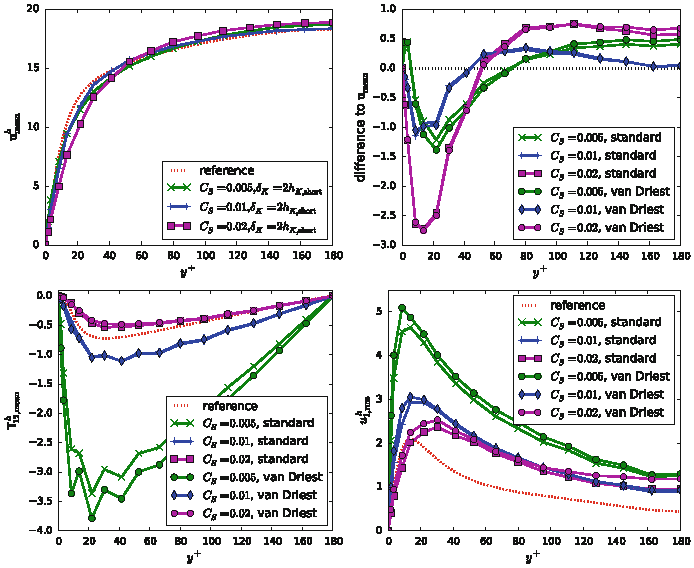
\includegraphics[width=\linewidth]{figures/Chapter_08/Fig_8_11__PDFp648__Bookp639.pdf}
\captionof{figure}{例题\hyperref[ex:vms-coarse-projection-channel-flow]{8.277}:采用 $\mathcal L^H=\mathbb P_0$ 的三尺度粗空间投影 VMS 方法\hyperref[eq:vms-coarse-projection-three-scale-method]{(8.288)}所得的若干统计量.}
\label{fig:vms-channel-p0-statistics}
\end{elegantfigure}

图\hyperref[fig:vms-channel-p0-statistics]{8.11}、\hyperref[fig:vms-channel-p1-statistics]{8.12}和\hyperref[fig:vms-channel-adaptive-statistics]{8.13}分别给出了 $\mathcal L^H=\mathbb P_0$、$\mathcal L^H=\mathbb P_1^{\mathrm{disc}}$ 以及自适应选取投影空间时,三尺度粗空间投影 VMS 方法\hyperref[eq:vms-coarse-projection-three-scale-method]{(8.288)}的结果.

正如笔记\hyperref[note:vms-dynamic-smagorinsky-common-goal]{8.216}所述,三尺度 VMS 方法的目标之一,是限制 Smagorinsky 模型直接作用于小的已解析尺度,从而降低该模型的影响.结果表明,这一目标确已实现:与 Smagorinsky 大涡模拟模型相比,该方法在更宽的 $C_S$ 参数范围内都能给出合理结果,见图\hyperref[fig:smagorinsky-channel-flow]{8.4}.VMS 方法在较大的 $C_S$ 取值下结果最准确.与 Smagorinsky 大涡模拟模型类似,采用 van Driest 阻尼\hyperref[eq:van-driest-damping]{(8.152)}的影响很小.标准 Smagorinsky 方法的结果往往略为准确,但并非总是如此.

\begin{elegantfigure}[1.055\linewidth]
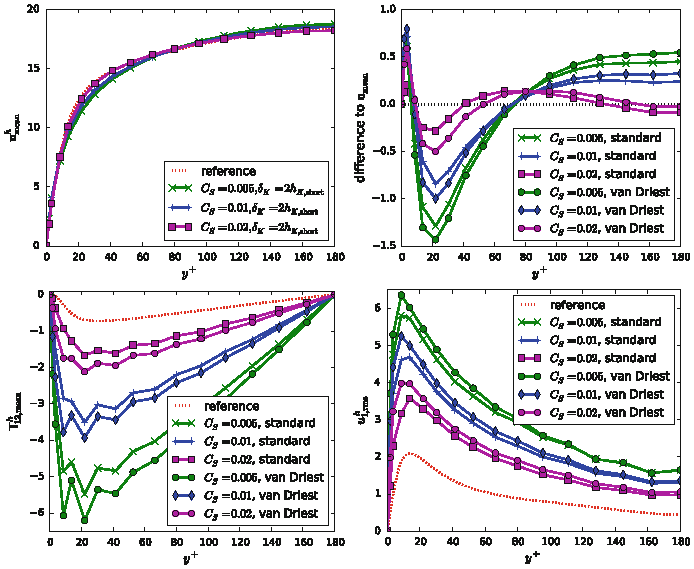
\includegraphics[width=\linewidth]{figures/Chapter_08/Fig_8_12__PDFp649__Bookp640.pdf}
\captionof{figure}{例题\hyperref[ex:vms-coarse-projection-channel-flow]{8.277}:采用 $\mathcal L^H=\mathbb P_1^{\mathrm{disc}}$ 的三尺度粗空间投影 VMS 方法\hyperref[eq:vms-coarse-projection-three-scale-method]{(8.288)}所得的若干统计量.}
\label{fig:vms-channel-p1-statistics}
\end{elegantfigure}

\begin{elegantfigure}[1.055\linewidth]
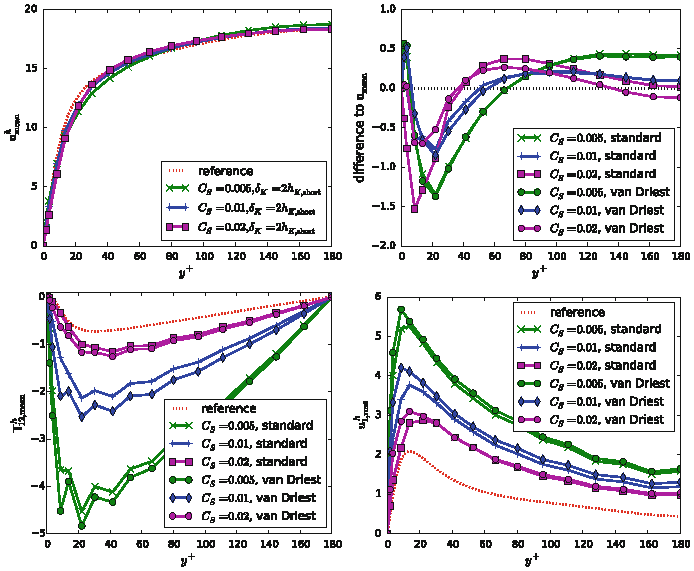
\includegraphics[width=\linewidth]{figures/Chapter_08/Fig_8_13__PDFp650__Bookp641.pdf}
\captionof{figure}{例题\hyperref[ex:vms-coarse-projection-channel-flow]{8.277}:自适应选取投影空间时,三尺度粗空间投影 VMS 方法\hyperref[eq:vms-coarse-projection-three-scale-method]{(8.288)}所得的若干统计量.}
\label{fig:vms-channel-adaptive-statistics}
\end{elegantfigure}
\end{example}
\index{变分多尺度方法!基于粗空间投影!实现}
\index{变分多尺度方法!基于粗空间投影!自适应投影空间}
\index{投影空间!自适应选取}



\section{若干湍流模型的数值比较}
\label{sec:comparison-turbulence-models}

\begin{note}[内容]
\label{note:comparison-turbulence-models-contents}
本节比较本章介绍的若干湍流模型所得到的数值解.重点讨论 Smagorinsky 模型和三尺度粗空间投影 VMS 方法,因为在 $\mathrm{Re}_\tau=180$ 的湍流槽道流中,这两种方法给出的结果最准确.对本节涉及的问题,采用有理 LES 模型、Leray-$\alpha$ 模型和 Navier--Stokes-$\alpha$ 模型进行模拟,通常无法得到令人满意的结果.
\end{note}

\begin{example}[($\mathrm{Re}_\tau=180$ 的湍流槽道流)]
\label{ex:vms-comparison-channel-180}
本例仅列出例题\hyperref[ex:smagorinsky-turbulent-channel]{8.128}和\hyperref[ex:vms-coarse-projection-channel-flow]{8.277}中所考察湍流模型的最佳参数:
\begin{itemize}
 \item Smagorinsky 模型\hyperref[eq:smagorinsky-filter-width]{(8.69)}(Smag):$\delta_K=2h_{K,\mathrm{short}}$,$C_S=0.005$,并采用 van Driest 阻尼\hyperref[eq:van-driest-damping]{(8.152)};
 \item 粗空间投影方法\hyperref[eq:vms-coarse-projection-three-scale-method]{(8.288)},其中 $\mathcal L^H=\mathbb P_0$(VMS0):$\delta_K=2h_{K,\mathrm{short}}$,$C_S=0.01$,不采用 van Driest 阻尼;
 \item 粗空间投影方法\hyperref[eq:vms-coarse-projection-three-scale-method]{(8.288)},其中 $\mathcal L^H=\mathbb P_1^{\mathrm{disc}}$(VMS1):$\delta_K=2h_{K,\mathrm{short}}$,$C_S=0.02$,不采用 van Driest 阻尼;
 \item 自适应选取投影空间的粗空间投影方法(VMSadap):$\delta_K=2h_{K,\mathrm{short}}$,$C_S=0.02$,并采用 van Driest 阻尼\hyperref[eq:van-driest-damping]{(8.152)}.
\end{itemize}
这些参数下的结果见图\hyperref[fig:vms-comparison-channel-180]{8.14}.在所比较的湍流模型中,VMS0 和 VMSadap 的结果最准确,而 Smagorinsky 模型的结果最不准确.

\begin{elegantfigure}[333.25pt]
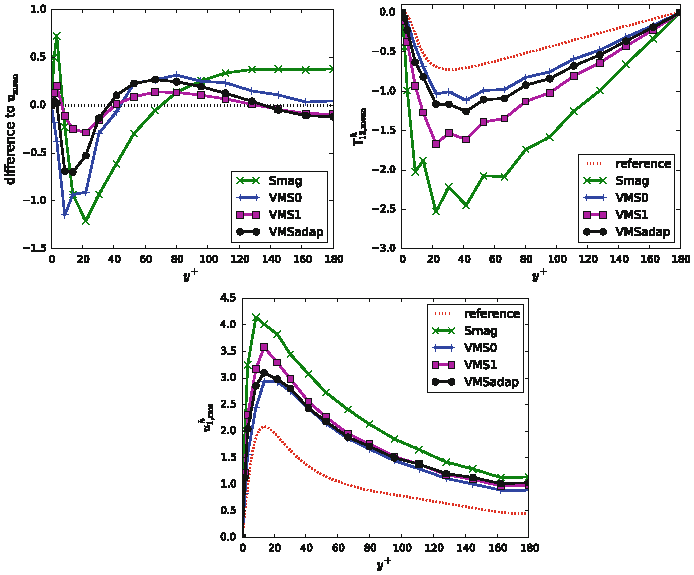
\includegraphics[width=333.25pt]{figures/Chapter_08/Fig_8_14__PDFp651__Bookp642.pdf}
\captionof{figure}{例题\hyperref[ex:vms-comparison-channel-180]{8.279}:$\mathrm{Re}_\tau=180$ 湍流槽道流中,Smagorinsky 模型和三尺度粗空间投影 VMS 模型采用最佳参数时的若干统计量.}
\label{fig:vms-comparison-channel-180}
\end{elegantfigure}
\end{example}

\begin{example}[($\mathrm{Re}_\tau=395$ 的湍流槽道流)]
\label{ex:vms-comparison-channel-395}
本例的说明见例题\hyperref[ex:appendix-d-12]{D.12}.模拟设置与 $\mathrm{Re}_\tau=180$ 的湍流槽道流相似,参见例题\hyperref[ex:smagorinsky-turbulent-channel]{8.128},只是空间网格和时间步长更细.空间网格由 $16\times16\times32$ 个单元组成.对 $Q_2/\mathbb P_1^{\mathrm{disc}}$ 有限元空间对,速度自由度为 199,680 个(包括 Dirichlet 节点),压力自由度为 32,768 个.Crank--Nicolson 格式的时间步长取 $\Delta t=0.002$.时间区间长度、靠近壁面的网格加密等其他设置均与例题\hyperref[ex:smagorinsky-turbulent-channel]{8.128}相同.

结果见图\hyperref[fig:vms-comparison-channel-395]{8.15}.VMS0 配合 $C_S=0.02$ 得到的结果最好.Smagorinsky 模型取 $C_S=0.01$、VMSadap 取 $C_S=0.02$ 时,也得到同样较好的结果.VMS1 取 $C_S=0.01$、Smagorinsky 模型取 $C_S=0.005$ 时,结果不准确.因此,针对 $\mathrm{Re}_\tau=180$ 湍流槽道流选出的 Smagorinsky 模型最佳参数,并不适用于本例.

\begin{elegantfigure}[333.5pt]
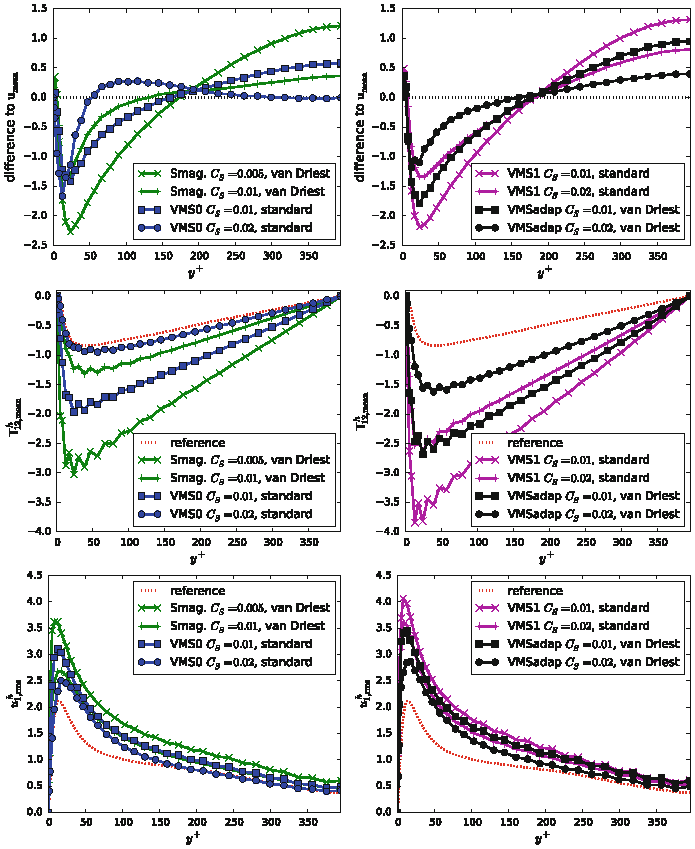
\includegraphics[width=333.5pt]{figures/Chapter_08/Fig_8_15__PDFp652__Bookp643.pdf}
\captionof{figure}{例题\hyperref[ex:vms-comparison-channel-395]{8.280}:$\mathrm{Re}_\tau=395$ 湍流槽道流中,Smagorinsky 模型和三尺度粗空间投影 VMS 模型所得的若干统计量.}
\label{fig:vms-comparison-channel-395}
\end{elegantfigure}
\end{example}

\begin{example}[($\mathrm{Re}=22{,}000$ 的绕圆柱湍流)]
\label{ex:vms-comparison-cylinder}
本例及其关注量见例题\hyperref[ex:appendix-d-13]{D.13}.模拟采用六面体网格和 $Q_2/\mathbb P_1^{\mathrm{disc}}$ 空间对;在第 2 层网格上,速度自由度为 522,720 个(包括 Dirichlet 节点),压力自由度为 81,920 个.图\hyperref[fig:vms-comparison-cylinder-grid]{8.16}给出了初始网格(第 0 层).时间离散采用等距步长 $\Delta t=0.005$ 的 Crank--Nicolson 格式.

\begin{elegantfigure}[226.5pt]
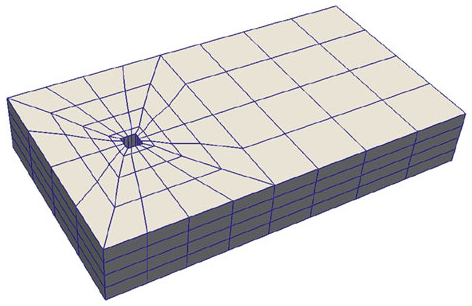
\includegraphics[width=226.5pt]{figures/Chapter_08/Fig_8_16__PDFp653__Bookp644.pdf}
\captionof{figure}{例题\hyperref[ex:vms-comparison-cylinder]{8.281}:初始网格,第 0 层.}
\label{fig:vms-comparison-cylinder-grid}
\end{elegantfigure}

本例不采用 van Driest 阻尼.所有流动均先发展 10 秒,随后在 30 个周期内计算统计量.

\begin{eleganttable}
\centering
\captionof{table}{例题\hyperref[ex:vms-comparison-cylinder]{8.281}}
\label{tab:vms-comparison-cylinder-statistics}
\scriptsize
\setlength{\tabcolsep}{2.5pt}
\renewcommand{\arraystretch}{1.16}
\resizebox{\linewidth}{!}{%
\begin{tabular}{l|c|cc|cc|c}
\hline
方法 & $C_S$ & $c_{\mathrm{lift}}$ & $c_{\mathrm{lift,rms}}$
 & $c_{\mathrm{drag}}$ & $c_{\mathrm{drag,rms}}$ & $\mathrm{St}$\\
\hline
Smag & 0.005 & \multicolumn{5}{c}{计算发散}\\
Smag & 0.01 & 0.001 & 1.46 & 2.58 & 0.11 & 0.151\\
Smag & 0.02 & 0.023 & 1.52 & 2.52 & 0.16 & 0.140\\
VMS0 & 0.01 & $-0.017$ & 1.28 & 2.60 & 0.19 & 0.139\\
VMS0 & 0.02 & $-0.015$ & 1.29 & 2.65 & 0.14 & 0.142\\
VMS1 & 0.01 & $-0.004$ & 1.04 & 2.49 & 0.15 & 0.136\\
VMS1 & 0.02 & $-0.026$ & 1.00 & 2.50 & 0.21 & 0.131\\
VMSadap & 0.01 & $-0.006$ & 1.15 & 2.49 & 0.21 & 0.131\\
VMSadap & 0.02 & $-0.026$ & 1.49 & 2.55 & 0.16 & 0.141\\
实验值 & & 0 & $[0.7,1.4]$ & $[1.9,2.1]$ & $[0.1,0.2]$ & 0.132\\
\hline
\end{tabular}%
}
\par\smallskip
\footnotesize 关注量的计算值及实验值.
\end{eleganttable}

表\hyperref[tab:vms-comparison-cylinder-statistics]{8.1}列出了所比较方法得到的结果.大多数结果在定性上相近:均方根(rms)值处于实验区间内,或仅略微超出该区间;平均阻力系数则明显高于实验值.文献中也经常报告后一现象,例如\textcite{GravemeierKronbichlerGeeWall2011,RasthoferGravemeier2013}.各方法所得 Strouhal 数之间则存在较明显差异:Smagorinsky 模型取 $C_S=0.01$ 时结果最差,VMS1 的结果最好.

\begin{elegantfigure}[226.5pt]
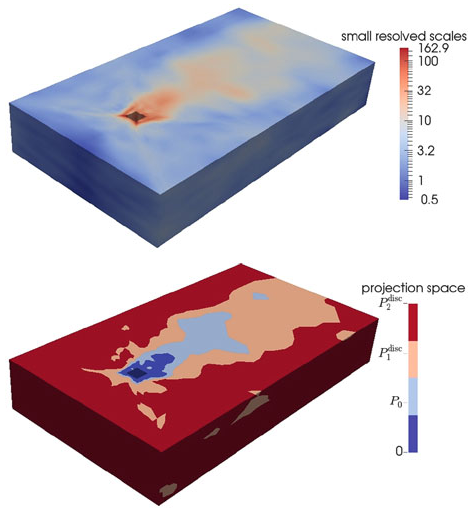
\includegraphics[width=226.5pt]{figures/Chapter_08/Fig_8_17__PDFp654__Bookp645.pdf}
\captionof{figure}{例题\hyperref[ex:vms-comparison-cylinder]{8.281}:自适应投影空间的三尺度投影 VMS 方法中,小的已解析尺度的大小(上)及相应投影空间(下).}
\label{fig:vms-adaptive-cylinder-flow}
\end{elegantfigure}

此外,Smagorinsky 模型取 $C_S=0.005$ 时发散,这一点值得注意.因此,该模型在 $\mathrm{Re}_\tau=180$ 湍流槽道流中的最佳参数在本例中失效.相较之下,本例也表明三尺度粗空间投影 VMS 方法对 $C_S$ 的选取不那么敏感.

图\hyperref[fig:vms-adaptive-cylinder-flow]{8.17}展示了小的已解析尺度的大小、空间分布以及自适应投影空间的相应选取.本例中,圆柱表面及其下游区域的湍流强度预计最高.图中小的已解析尺度的大小与这一预期相符,因此式\hyperref[eq:vms-coarse-projection-local-turbulence-intensity]{(8.328)}中的 $\zeta_K$ 是合适的局部湍流强度估计量.从投影空间图中可以看出,湍流模型在圆柱处的影响最大,沿下游方向逐渐减弱,在其他区域则基本关闭.
\end{example}

\begin{example}[($\mathrm{Re}=40{,}000$ 的壁装立方体绕流)]
\label{ex:vms-comparison-wall-mounted-cube}
本问题见例题\hyperref[ex:appendix-d-14]{D.14}.

\begin{elegantfigure}[226.5pt]
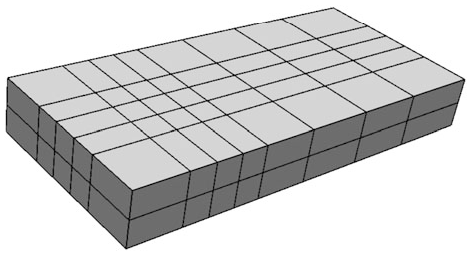
\includegraphics[width=226.5pt]{figures/Chapter_08/Fig_8_18__PDFp655__Bookp646.pdf}
\captionof{figure}{例题\hyperref[ex:vms-comparison-wall-mounted-cube]{8.282}:初始网格,第 0 层.}
\label{fig:vms-comparison-wall-mounted-cube-grid}
\end{elegantfigure}

数值模拟采用六面体网格上的 $Q_2/\mathbb P_1^{\mathrm{disc}}$ 空间对.初始网格(第 0 层)见图\hyperref[fig:vms-comparison-wall-mounted-cube-grid]{8.18},表\hyperref[tab:vms-comparison-wall-mounted-cube-dofs]{8.2}列出了自由度数量.模拟时间区间为 $[0,10]$,时间离散采用等距步长 $\Delta t=0.01$ 的 Crank--Nicolson 格式.计算阻力系数的时间平均值时,取区间 $[5,10]$.所有湍流模型均未采用 van Driest 阻尼.

\begin{eleganttable}[0.68\linewidth]
\centering
\captionof{table}{例题\hyperref[ex:vms-comparison-wall-mounted-cube]{8.282}}
\label{tab:vms-comparison-wall-mounted-cube-dofs}
\scriptsize
\setlength{\tabcolsep}{4pt}
\renewcommand{\arraystretch}{1.12}
\begin{tabular}{c|rrr}
\hline
层级 & 速度 & 压力 & 总计\\
\hline
2 & 134,739 & 20,224 & 154,963\\
3 & 1,023,651 & 161,792 & 1,185,443\\
\hline
\end{tabular}
\par\smallskip
\footnotesize 空间自由度数(包括 Dirichlet 节点).
\end{eleganttable}

\begin{eleganttable}[0.82\linewidth]
\centering
\captionof{table}{例题\hyperref[ex:vms-comparison-wall-mounted-cube]{8.282}}
\label{tab:vms-comparison-wall-mounted-cube-drag}
\scriptsize
\setlength{\tabcolsep}{4pt}
\renewcommand{\arraystretch}{1.12}
\begin{tabular}{l|c|cc}
\hline
方法 & $C_S$ & 第 2 层 & 第 3 层\\
\hline
Smag & 0.005 & 1.16 & 1.46\\
Smag & 0.01 & 1.26 & 1.45\\
VMS0 & 0.01 & 1.19 & 1.47\\
VMS0 & 0.02 & 1.23 & 1.45\\
VMS1 & 0.01 & 1.09 & 1.39\\
VMS1 & 0.02 & 1.11 & 1.38\\
VMSadap & 0.01 & 1.13 & 1.37\\
VMSadap & 0.02 & 1.21 & 1.33\\
\hline
\end{tabular}
\par\smallskip
\footnotesize 平均阻力系数;参考值 $c_{\mathrm{drag}}\approx1.5$.
\end{eleganttable}

表\hyperref[tab:vms-comparison-wall-mounted-cube-drag]{8.3}给出了不同湍流模型的结果.图\hyperref[fig:vms-comparison-wall-mounted-cube-drag]{8.19}以两种模型为例,展示了计算所得阻力系数随时间的变化.可以看到,所有湍流模型在较粗的第 2 层网格上都低估了平均阻力系数.在较细的第 3 层网格上,Smagorinsky 模型和 VMS0 所得平均阻力系数与参考值处于同一量级;VMS1 和 VMSadap 仍明显低估这一系数.图\hyperref[fig:vms-comparison-wall-mounted-cube-drag]{8.19}还表明,在较细网格上,计算阻力系数围绕其平均值的振荡幅度显著减小.

\begin{elegantfigure}[333.25pt]
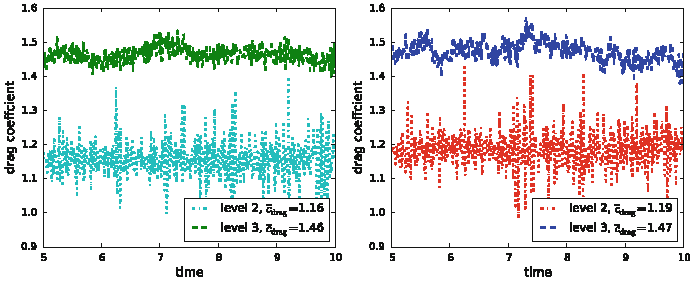
\includegraphics[width=333.25pt]{figures/Chapter_08/Fig_8_19__PDFp656__Bookp647.pdf}
\captionof{figure}{例题\hyperref[ex:vms-comparison-wall-mounted-cube]{8.282}:Smagorinsky 模型 $C_S=0.005$(左)和 VMS0 $C_S=0.01$(右)所得阻力系数.}
\label{fig:vms-comparison-wall-mounted-cube-drag}
\end{elegantfigure}
\end{example}

\index{湍流模型!数值比较}
\index{Smagorinsky 模型!与 VMS 方法比较}
\index{变分多尺度方法!基于粗空间投影!数值比较}

